\documentclass[12pt,a4paper,violet]{bbe}
\usepackage{blindtext}
\usepackage{fontspec}
\usepackage{tabularx}
\usepackage{csvsimple}
\usepackage{tabularx}
\setmainfont[Script=Myanmar]{Pyidaungsu}
\setcounter{tocdepth}{4}
\setcounter{secnumdepth}{4}

\title{Introduction to Deep Learning}
\authors{Dr. Myo Thida } % Use \authors instead of \author due to your custom command
%\date{Date Here}


\begin{document}
%\maketitle

\thispagestyle{empty}

\begin{tikzpicture}[remember picture,overlay]
    \node at (current page.center) {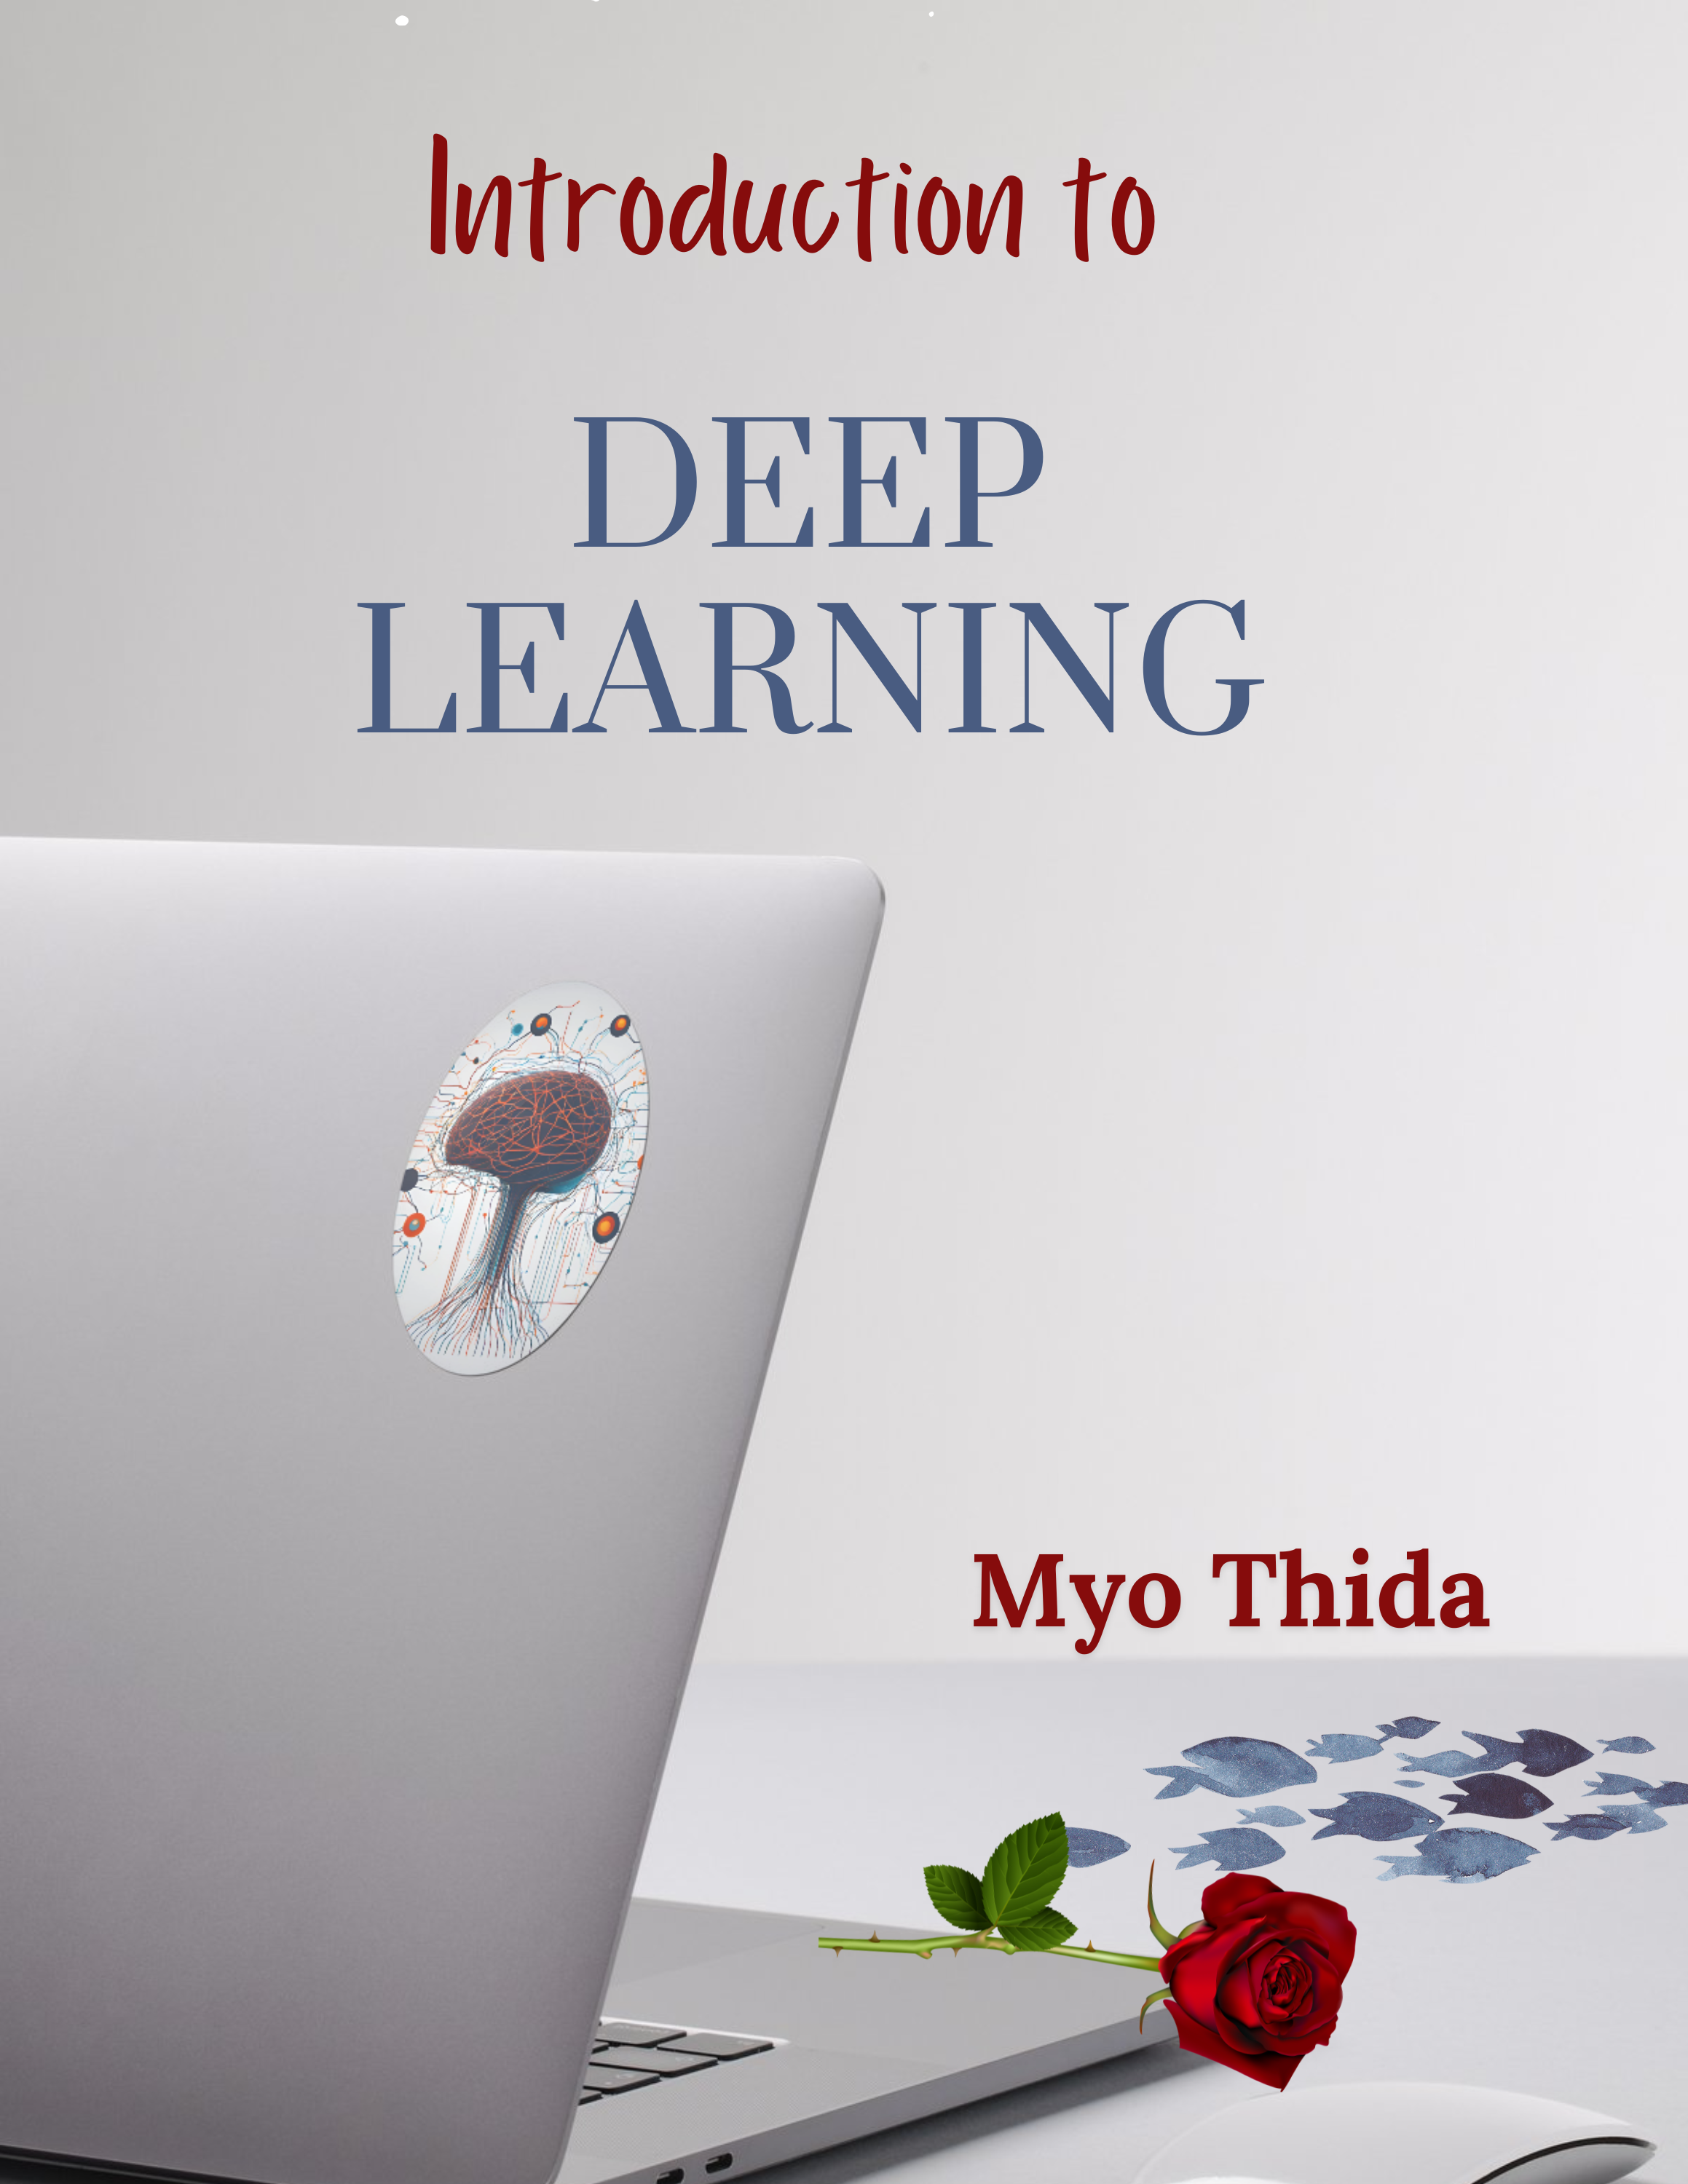
\includegraphics[width=\paperwidth,height=\paperheight]{imgs/DL_cover3.png}};
    %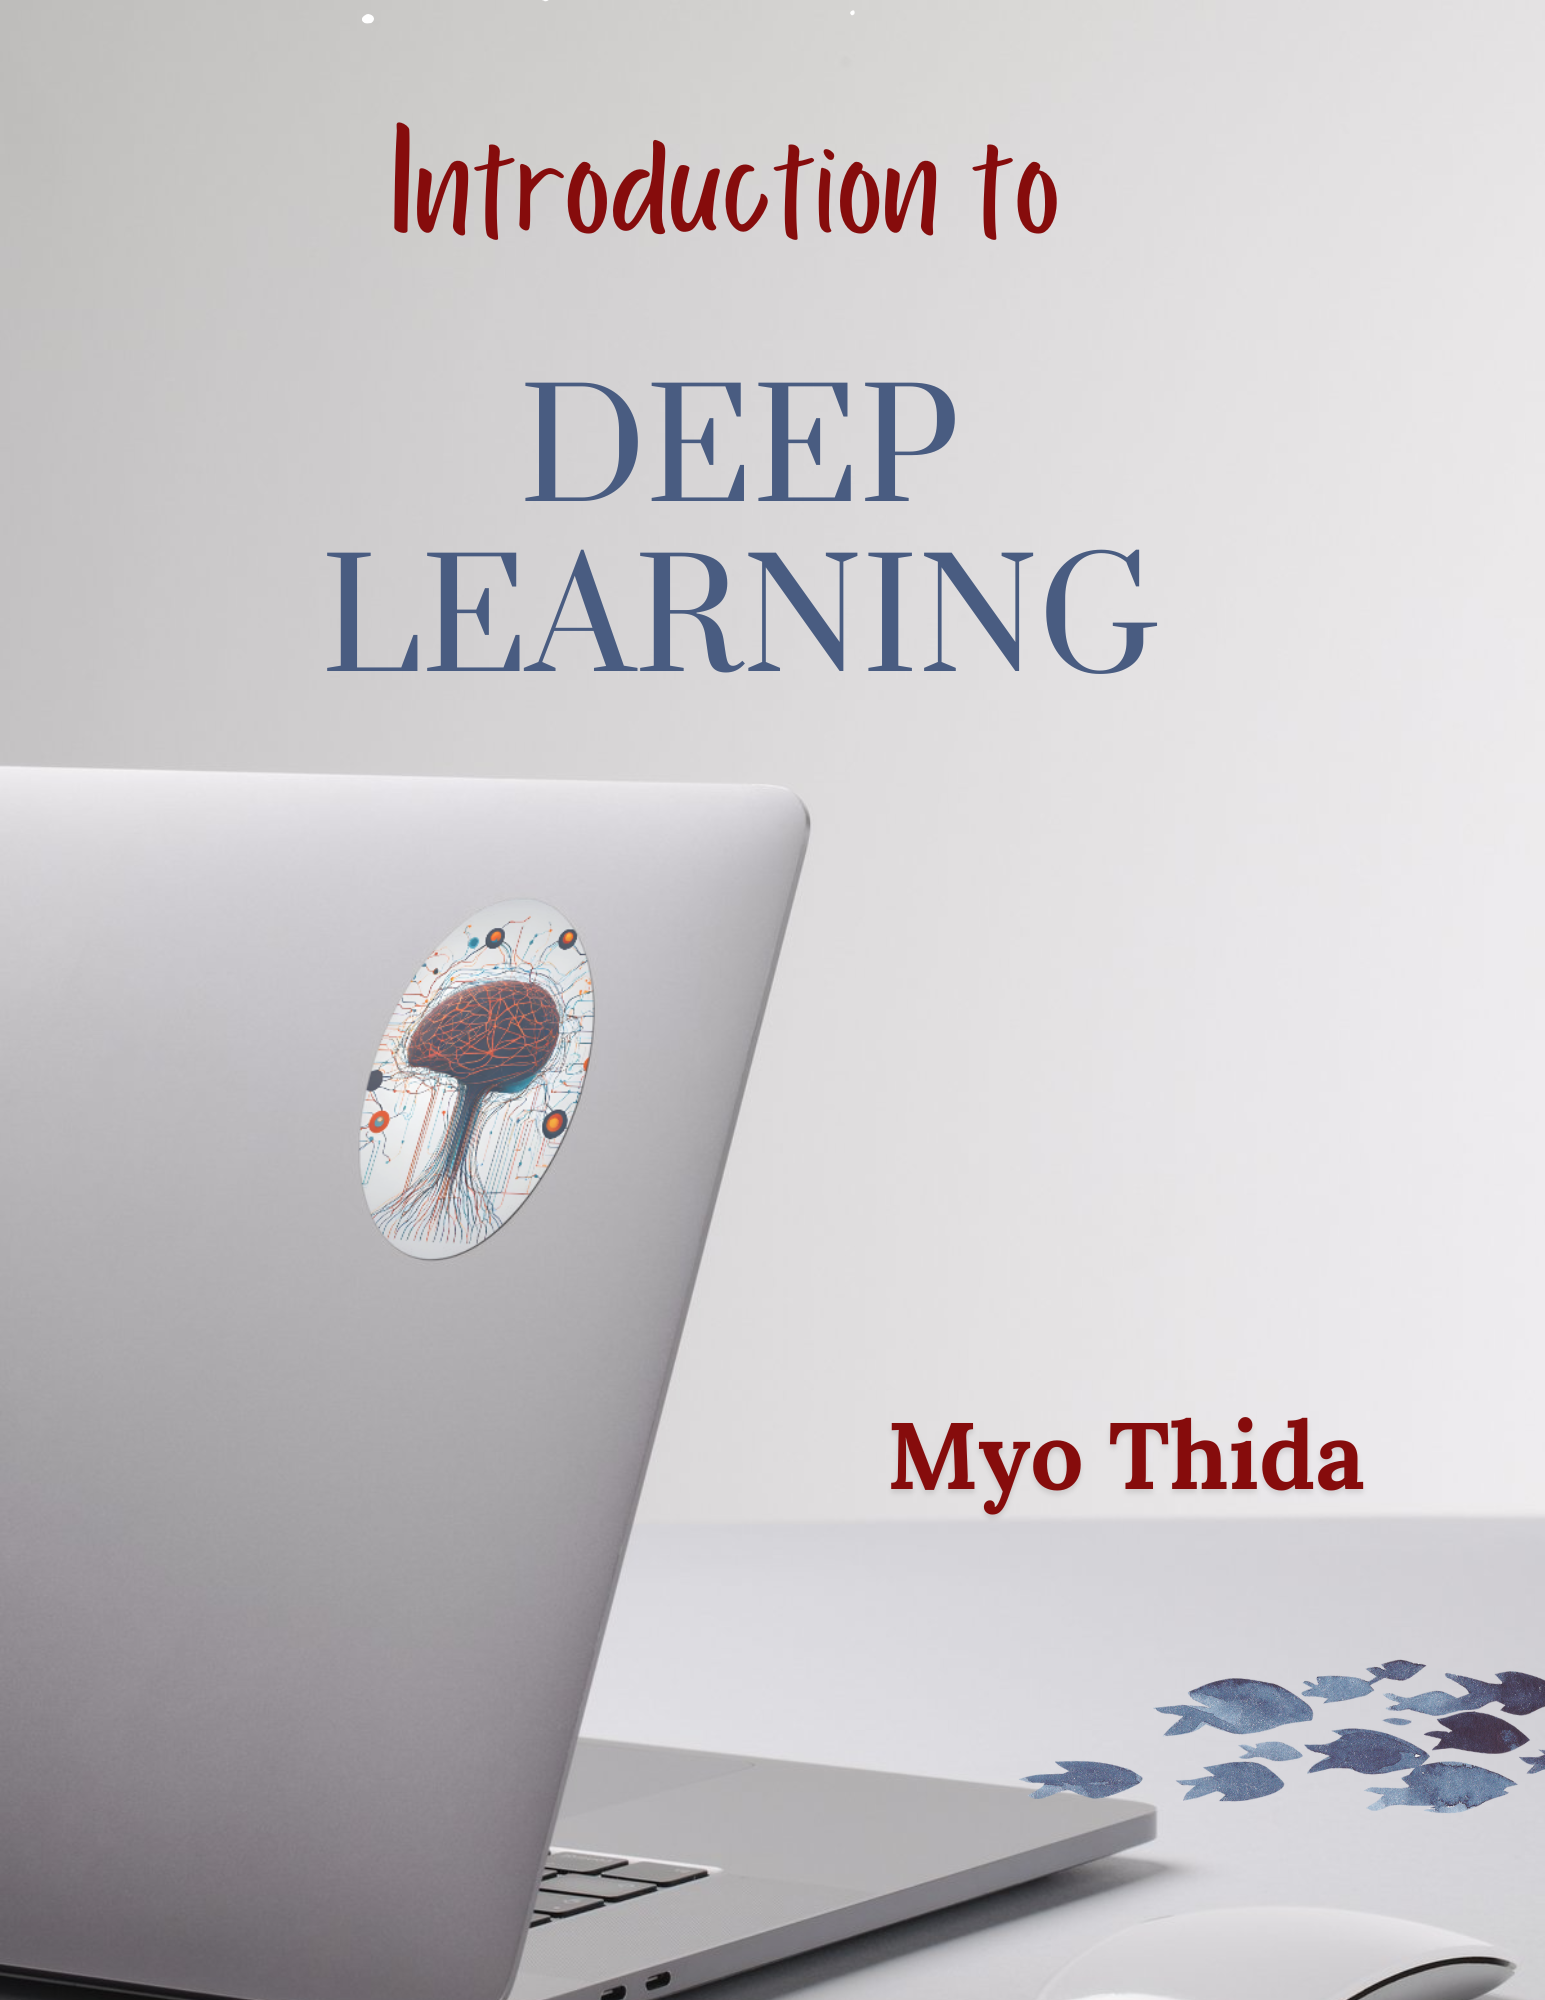
\includegraphics[width=\paperwidth]{imgs/DL_cover.png}
\end{tikzpicture}

\newpage
\thispagestyle{empty}
\vspace*{9cm}
\begin{center}
   \emph{\color{darkgray}This book is dedicated to my students over the years and to the brave youths of Myanmar, who have infused me with unwavering courage and energy, inspiring me to persevere.}
\end{center}


\newpage 
\thispagestyle{empty}
\vspace*{\fill}
\small
Copyright \textcopyright\ 2024 by VigorZwe Co. Ltd. All rights reserved.
No part of this book may be reproduced or reprinted without permission in writing from the publisher or the author.
\clearpage 
\pagenumbering{roman}
\setcounter{page}{1} % Reset page counter to 1

\thispagestyle{empty}
\chapter*{Preface}

%The terms 'AI,' 'deep learning,' and 'machine learning' are not unfamiliar to me, as I am trained as a computer vision and machine learning scientist. My PhD research, which focused on analyzing the contextual information of videos using traditional machine learning techniques, remains relevant, with many readers still citing it as foundational work. However, I took a career hiatus of approximately six years to contribute to the national development of Myanmar. Upon returning to the technological landscape in 2019, I experienced stress and anxiety, fearing I had fallen behind.
%
%Determined to catch up, I quickly familiarized myself with new terminologies and found learning to be more manageable, perhaps due to my increased maturity and experience collaborating with industry professionals. This newfound clarity enabled me to communicate complex concepts more effectively, as evidenced by the success of my previous work, 'Introduction to Supervised Machine Learning (2023),' which sold over 100 copies within a year. Moreover, receiving positive feedback from readers about the accessibility and clarity of my explanations motivated me to embark on writing this teaching book: 'Introduction to Deep Learning.'

My interest in AI began in 2003 when I completed a literature review on face recognition methods as my first undergraduate research project. This project sparked my passion for computer vision and machine learning, leading me to pursue both a Master's and a PhD in the field. Throughout my academic journey, I published research in journals and authored a book titled 'Contextual Analysis of Videos,' all written in English.

Over time, I became aware of the challenges faced by many Myanmar students, who had limited access to quality books due to language barriers and found most available resources too advanced. This realization inspired me to write technology books in Burmese using my own teaching style. My first book, 'Introduction to MATLAB: Learning by Doing,' was published in 2008. The second book, 'Introduction to Supervised Machine Learning,' written in both English and Burmese, was published in 2023. Encouraged by positive feedback on the accessibility and clarity of my explanations, I embarked on writing this teaching book: 'Introduction to Deep Learning.'

This book emerged from one of the most challenging periods of my life, during which the tumultuous situation in Myanmar weighed heavily on my mind, particularly witnessing the struggles of many young people. The purpose of this book is not only to make deep learning accessible to students with limited resources but also to contribute to the support of youths in need. 

This book is structured into four parts to facilitate a comprehensive understanding of deep learning concepts and methodologies. The first chapter serves as a foundational introduction to deep machine learning algorithms. It covers the historical evolution of deep learning, essential mathematical concepts, and prerequisites necessary to comprehend the subsequent chapters.  It also introduces Python libraries commonly used for deep learning, such as TensorFlow and Keras.

Chapter two delves into the architecture and functioning of shallow neural networks. It covers topics such as activation functions, forward and backward propagation, and model optimization techniques. Practical projects demonstrating the application of shallow NNs in regression, binary classification, and multi-class classification tasks are included.  Chapter three explores advanced deep learning architectures, including convolutional neural networks (CNNs), recurrent neural networks (RNNs), and their variants. It discusses the principles behind these architectures and their applications in computer vision, natural language processing, and time-series data analysis.

Chapter four delves into specialized topics and emerging trends in deep learning. It covers areas such as transfer learning, attention mechanisms, AutoML, neural architecture search (NAS), and ethical considerations in deep learning. Through case studies and discussions, this chapter provides insights into advanced methodologies and ethical considerations shaping the future of deep learning.

I believe that hands-on learning is crucial for understanding, and thus, the explanations in the book are accompanied by detailed 'Python code' snippets throughout the text. Readers can follow the instructions and run the code on their own computer or an online platform such as Google Colab.

As you delve into the chapters that follow, I encourage you to approach this journey with an open mind and a spirit of exploration. Whether you are a seasoned expert in the field or a curious novice, there is something to be gained from the insights contained within these pages.

The website: \href{www.drmyothida.org/courses}{www.drmyothida.org/courses/machinelearning}. The complete code for all the projects in this book is also available on the public \href{https://github.com/myothida/Intro-To-Supervised-Machine-Learning.git}{\textbf{GitHub Repo}}.

\chapter*{စာညွှန်း}

စာရေးသူမှာ စင်ကာပူနိုင်ငံ နန်ယန်း တက္ကသိုလ်တွင် အင်ဂျင်နီယာ ဘွဲ့ကြိုသင်တန်းအား ၂၀၀၁ မှ ၂၀၀၅ ခုနှစ်ထိ တတ်ရောက်ခဲ့ပါသည်။ ထိုဘွဲ့ကြိုသင်တန်းကာလအတွင်း ပြုလုပ်ခဲ့သည့် "Literature Review on Face Recognition Methods" ဟုခေါ်ဆိုသည့် စာတမ်းငယ် မှာ စာရေးသူ၏ ပထမဦးဆုံး မှတ်ဥာဏ်အတု Artificial Intelligence (AI) နှင့် ပတ်သတ်သည့် သုတေသန လုပ်ငန်းစဥ် တစ်ခု ဖြစ်ခဲ့ပါသည်။ ထိုသုတေသနမှ အစပြု၍ computer vision နှင့် machine learning ကို ပိုမို စိတ်၀င်စားလာကာ Computer Vision ဘာသာရပ်ကို အထူးပြု၍ မာစတာနှင့် ဒေါက်တာ ဘွဲ့များကို ဆက်လက် ရယူခဲ့ပါသည်။ သုတေသန စာတမ်းငယ်များစွာနှင့် Contextual Analysis of Videos နည်းပညာစာအုပ်ကို အင်္ဂလိပ်ဘာသာဖြင့်  ရေးသား ထုတ်၀ေခဲ့သည်။

၂၀၁၃ ခုနှစ် နှောင်းပိုင်းတွင် မြန်မာနိုင်ငံသို့ ပြန်ရောက်ပြီးနောက် မြန်မာလူငယ်များကို   computer vision နှင့် machine learning ဆိုင်ရာ ဘာသာရပ်များကို သင်ကြားဖြစ်ရင်းမှ အင်္ဂလိပ်ဘာသာစကားဖြင့် ထုတ်၀ေသည့် စာအုပ်များကို မြန်မာ လူငယ်များ (အထူးသဖြင့် အင်္ဂလိပ်စာ ဘာသာစကား အားနည်းသော လူငယ်များ ) အတွက် ဖတ်ရှု့လေ့လာရန် ခက်ခဲလျက်ရှိသည်ကို သိရှိလာရသည်။ သို့ဖြစ်ရာ ရိုးရှင်းသည့် စကားလုံးများကို အသုံးပြု၍ မြန်မာသာသာဖြင့် နည်းပညာစာအုပ်များကို သင်ကြားရေးတွင် အသုံးပြုရန် စတင် ရေးသားခဲ့ပါသည်။ ထို့နောက် ၂၀၁၈ ခုနှစ်တွင် Introduction to MATLAB: Learning by Doing စာအုပ်ကို လည်းကောင်း၊ ၂၀၂၃ ခုနှစ်တွင်  Introduction to Supervised Machine Learning စာအုပ်ကို လည်းကောင်း ရေးသားထုတ်၀ေခဲ့သည်။ 

ယခု ရေးသားထုတ်၀ေမည့် Introduction to Deep Learning နှင့်  ၂၀၂၃ ခုနှစ်တွင် ထုတ်၀ေခဲ့သည့် Introduction to Supervised Machine Learning - စာအုပ် ၂ အုပ်လုံးမှာ ကျွန်မ ဘ၀၏ စိတ်သောက အများဆုံး အချိန်တွင် ရေးသားခဲ့သည့် စာအုပ်များဖြစ်သည်ဟု ဆိုနိုင်ပါသည်။ လက်ရှိ မြန်မာနိုင်ငံ၏ အခြေအနေများမှာ ပညာရေးဖြင့် တိုင်းပြည်ကို တိုးတက်စေချင်သူ ကျွန်မအတွက် စိတ်ဖိစီးမှု များစွာ ဖြစ်စေပါသည်။ သို့သော် ခက်ခဲနေသည့် အခြေအနေများ အကြားတွင်ပင် မလျှော့သော ဇွဲ၊ လုံ့လဖြင့် ကြိုးစားနေကြသည့် မြန်မာ လူငယ်များမှ ပေးသောခွန်အားဖြင့် ဤနည်းပညာစာအုပ်များကို ရေးသားခဲ့ပါသည်။  ယခု စာအုပ်သည် အခြားနိုင်ငံသားများနည်းတူ မြန်မာ လူငယ်များလည်း နည်းပညာကို အမီလိုက်နိုင်စေရန် ရည်ရွယ်ရေးသားခြင်း ဖြစ်သည်။ နှလုံးသားနှင့် ဦးဏှောက် စည်းချက်ညီစွာဖြင့် ကြိုးစားနေကြသော မြန်မာ လူငယ်၊ လူရွယ် (ဆယ်လ်မွန်ငါး) များအတွက် အလွယ်တကူ ဖတ်ရှု့နိုင်သည့် နည်းပညာ စာအုပ်တစ်အုပ်အဖြစ် ပညာဖြန့်၀ေနိုင်ရန် ရည်ရွယ်ပါသည်။ 

ယခု စာအုပ်တွင် အပိုင်း ၄ ပိုင်းပါ၀င်ပြီး ပထမ အပိုင်းမှာ Deep Learning ကို မိတ်ဆက်ခြင်း ဖြစ်ပါသည်။ သို့သော် Machine Learning / AI စသည့် အခြေခံ သဘောတရားများကို ပြန်လည်ရှင်းပြခြင်းထက်  Deep Learning ၏ သဘောတရားများကို တိုက်ရိုက်မိတ်ဆက်သွားမည် ဖြစ်ရာ AI / Machine Learning စသည့် နည်းပညာ စကားလုံးများနှင့် ၀ေးကွာနေသူများအဖို့  ဤစာအုပ်ကိုမဖတ်မီ  Introduction to Supervised Machine Learning ကို ဖတ်ရှု့ရန် တိုက်တွန်းပါသည်။ Deep Learning ကို လေ့လာရာတွင် အရေးကြီးသည့် အချို့ သင်္ချာ ခေါင်းစဥ်များနှင့် ယခု စာအုပ်တွင် အသုံးပြုသွားမည့်  Python Library များကိုလည်း ပထမ အပိုင်းတွင် မိတ်ဆက်ထားပါသည်။ 

ဒုတိယအခန်းတွင်  Deep Learning ၏ မူလ အခြေခံဖြစ်သည့် Shallow Neural Network ကို ရှင်းပြသွားမည်ဖြစ်ပြီး လက်တွေ့ လေ့ကျင့်ခန်းများကို လည်း Python Code များနှင့်အတူ ဆွေးနွေးပေးသွားမည် ဖြစ်သည်။ ထို့နောက် တတိယ အခန်းတွင်မူ ပိုမို အဆင်မြင့်သည့် Deep Learning Architecture အမျိုးမျိုးကို ရှင်းလင်းသွားပြီး Convolutional Neural Networks (CNNs)၊ Recurrent Neural Networks (RNNs) များကို အသုံးပြု၍ Image များ  Text များကို အမျိုးအစား ခွဲခြားပုံများကို ဆွေးနွေးသွားပါမည်။ နောက်ဆုံးအပိုင်းတွင်မူ Deep Learning ၏ နောက်ဆုံး ပြောင်းလဲလျက်ရှိသည့် ခေါင်းစဥ်များနှင့် ဆက်လက်လေ့လာရမည်များကို ဆွေးနွေးသွားပါမည်။ 

ယခု စာအုပ်ကို အင်္ဂလိပ် - မြန်မာ ၂ ဘာသာဖြင့် ရေးသားထားပြီး စာမျက်နှာအလိုက် တွဲ၍ ဖတ်ရှု့သွားနိုင်မည် ဖြစ်သည်။ တိုက်ရိုက် ဘာသာပြန်ဆိုထားခြင်း မဟုတ်ဘဲ စာသားပြေပြစ်စေရန် အဓိက ရေးသားထားသည် ဖြစ်ရာ ဘာသာစကား တစ်ခုထဲကို အသုံးပြု ဖတ်ရှု့သူများ အနေဖြင့် အကျိုးရှိနိုင်သကဲ့သို့ ဘာသာစကား ၂ ခုလုံးကို တွဲ၍ ဖတ်ရှု့ပါကလည်း ပို၍ အကျိုးများနိုင်ပါသည်။ 

နည်းပညာစာအုပ်များကို ဖတ်ရှု့ရာတွင် အမှန်တကယ် နားလည်လိုသည်ဆိုပါက လက်တွေ့ လေ့ကျင့်ခန်းများနှင့် တွဲ၍ ဖတ်ရှု့ရန် လိုအပ်ပါသည်။ ဤစာအုပ်တွင် ပါရှိသည့် Python ဖြင့်ရေးသားထားသည့် လေ့ကျင့်ခန်းများကို အောက်ပါ \href{https://github.com/myothida/Intro-To-Supervised-Machine-Learning.git}{\textbf{GitHub}} လင့်တွင် ၀င်ရောက်၍ download ရယူပြီးလေ့ကျင့်စေလိုပါသည်။ 

\thispagestyle{empty}
\tableofcontents % Prints the table of contents


\clearpage 
\pagenumbering{arabic} % Switch to arabic page numbering for the main content
\setcounter{page}{1}

\chapter{Introduction to Deep Learning}
\label{ch:intro}

Deep learning, a subset of machine learning techniques, has revolutionized artificial intelligence (AI) in recent years. One prominent example of deep learning models is the Generative Pre-trained Transformer (GPT), which has attracted the attention not only of tech enthusiasts but also the general public. GPT models, like the ones developed by OpenAI \cite{web:chatgpt} , have demonstrated remarkable capabilities in natural language processing tasks, from text generation to translation, illustrating the transformative potential of deep learning.

Rooted in the concept of artificial neural networks (ANNs), deep learning models are inspired by the structure and function of the human brain, enabling them to learn from vast amounts of data and perform complex tasks with remarkable accuracy. Unlike traditional machine learning algorithms that require handcrafted feature extraction, deep learning models automatically learn hierarchical representations of data through these layers, enabling them to discover patterns and relationships.

However, this deep architecture introduces significant complexity, making it challenging to understand and optimize model performance. Additionally, deep learning models are resource-intensive, requiring substantial computational power for both training and inference. This requirement can limit their practical applicability, particularly in environments with limited computing resources or strict latency constraints.

Moreover, deep learning models often struggle with interpretability, which makes it difficult to understand and trust their decisions. This issue is particularly concerning in high-stakes applications such as health care, finance, and autonomous driving, where decision-making transparency is crucial. For instance, in medical diagnostics, understanding why a model made a specific recommendation is essential for gaining trust from health care professionals and patients alike.

\noindent
\vskip  1.0em
ယနေ့ခတ်တွင် လူအများစုက Deep learning နှင့်  Machine learning ကို နှိုင်းယှဥ်ပြောဆိုမှုများ ပြလုပ်လေ့ရှိကြပြီး Deep learning သည်  Machine learning ထက်သာသည်ဟု ပြောဆိုမှုများလည်း ရှိကြပါသည်။ သို့သော်လည်း Deep learning ဆိုသည်မှာ  Machine learning အမျိုးအစားတစ်ခုသာ ဖြစ်သည်။ မူလ traditional Machine learning များတွင် အားသာချက် ၊ အားနည်းချက်များ ရှိသကဲ့သို့ Machine learning  အမျိုးအစားတစ်ခုသာ ဖြစ်သည့် Deep learning model များတွင်လည်း အားသာချက်များ ၊ အားနည်းချက်များ ရှိပါသည်။ သို့သော် Deep learning model များသည် artificial intelligence (AI) လောကကို လူအများပိုမို စိတ်၀င်စားအောင် ဖန်တီးပေးခဲ့သည်မှာတော့ အမှန်ပင် ဖြစ်သည်။  ဥပမာ -- နည်းပညာသမားများသာမက နည်းပညာ နှင့် အလှမ်း၀ေးကွာသူများ၏ စိတ်၀င်စားမှုကိုပင် ရယူနိုင်ခဲ့သည့် ChatGPT အပါအ၀င် GPT model များသည် Deep Learning models များကို အခြေခံ၍ တည်ဆောက်ထားခြင်း ဖြစ်သည်။

Deep learning Model များသည် လူသား ဦးဏှောက် များ၏ လုပ်ဆောင်ပုံကို နမူနာယူ၍ တည်ဆောက်ထားသော  artificial neural networks များကို အခြေခံထားသည်။ မူလ traditional machine learning algorithm များနှင့် နှိုင်းယှဥ်မည် ဆိုပါက Deep learning Model များ၏ အဓိက အားသာချက်မှာ အချက်အလက်များ၏ ဆက်နွယ်ပုံ နှင့် အရေးပါသည့် အချက်အလက်များကို algorithm ရေးသူမှ ရှာဖွေရမည့်အစား  အချက်အလက်အမြောက်အများကို အသုံးပြု၍ အလိုအလျောက်ရှာဖွေခြင်းဖြစ်သည်။ သို့သော် ထိုအချက်သည်ပင် Deep learning Model များ၏ အားနည်းချက် တစ်ခုလည်း ဖြစ်သည်။ Deep learning Model တစ်ခု တည်ဆောက်ရန်အတွက် အချက်အလက် အမြောက်အမြားလိုအပ်ပြီး computational Power မြင့်သည့် ကွန်ပြူတာများ ၊ ဆာဗာများကိုလည်း လိုအပ်သည်။ သို့ဖြစ်ရာ computing Power မြင့်သည့် ကွန်ပြူတာများ ၊ ဆာဗာများကို မတတ်နိုင်သည့် သူများအတွက် Deep learning Model တစ်ခုကို ကိုယ်ပိုင် တည်ဆောက်ရန် ခက်ခဲလှသည်။

ထို့အပြင် Deep learning Model များ၏ အခြား ပြဿနာတစ်ခုမှာ မည်သည့်အတွက်ကြောင့် အဖြေမှန်(သို့မဟုတ်) ရလဒ်ကောင်းများ ရရှိသည်ကို တိတိကျကျ နားလည်ရန် နှင့် ရှင်းပြရန် မလွယ်ကူခြင်း ဖြစ်သည်။ သို့ဖြစ်ရာ  အသက်နှင့် လောင်းကြေးထပ်ရမည့် အလိုအလျောက် ကားမောင်းသည့် စနစ်များ၊ ကျန်းမာရေးဆိုင်ရာ ဆုံးဖြတ်ချက်များ နှင့် ငွေကြေးဆုံးရှုံးမှု မြင့်မားသည့် finance ကိစ္စရပ်များတွင် Deep learning Model များ၏ ဆုံးဖြတ်ချက်ကို သာမာန် နည်းပညာ အသုံးပြုသူများအနေဖြင့် အပြည့်အ၀ လက်ခံနိုင်ရန် ခက်ခဲနေဆဲဖြစ်သည်။


\section{History of Deep Learning}
\label{sec:history}
The basic idea of deep learning dates back to the 1940s and 1950s when researchers began exploring the mathematical models of neurons. A significant advancement occurred in the 1980s with Yann LeCun's work, particularly his development of convolutional neural networks (CNNs) \cite{lecun1989}, which played a crucial role in pushing the boundaries of neural network research. Despite these advancements, the field faced considerable challenges, such as limited computational power and insufficient data, leading to a period of stagnation during the 1970s and 1980s.

The breakthroughs that led to the modern era of deep learning began around the mid-2000s. The term ``deep learning" gained widespread recognition around 2012 when deep neural networks, particularly convolutional neural networks (CNNs)  \cite{krizhevsky2012ImageNet}, achieved ground-breaking performance in computer vision tasks, such as image classification, through competitions like the ImageNet Large Scale Visual Recognition Challenge (ILSVRC) \cite{web:ILSVRC}.

၁၉၄၀ ခုနှစ်များတွင် သုတေသနပညာရှင်များက လူသားများ၏ ဦးဏှောက်အတွင်းရှိ neuron များ အလုပ်လုပ်ပုံ၊ ဆုံးဖြတ်ချက်ချပုံများကို သင်္ချာ model များဖြင့် ဖော်ပြနိုင်ရန် ကြိုးစားခဲ့ကြခြင်းသည် Deep Learning ၏ အစပင် ဖြစ်သည်။
သို့သော် ထိုကာလများတွင် သုတသနလုပ်ငန်းများ၏ အဓိက ရည်ရွယ်ချက်မှာ လူသားဦးဏှောက်နှင့် ပုံစံတူ မော်ဒယ်များ တည်ဆောက်ရန်  ဖြစ်သည်။ ၁၉၈၉ ခုနှစ်တွင် သုတေသနပညာရှင် Yann LeCun က convolutional neural networks (CNNs) ကို တီထွင်ခဲ့ရာမှ ၄င်းသုတေသနကို အခြားနယ်ပယ်များတွင်ပါ အသုံးပြုရန် ပိုမိုစိတ်၀င်စားလာခဲ့ကြသည်။ သို့သော် computing Power နှင့် ဒေတာ အချက်အလက်များ မလုံလောက်ခြင်းတို့ကြောင့် neural network ၏ သုတေသနမှာ ယာယီရပ်တန့်ခဲ့ရသည်။

နှစ်စဥ်ကျင်းပလေ့ရှိသည့် ImageNet ခေါ် image များကို အမျိုးအစားခွဲခြားခြင်း ပြိုင်ပွဲ (၂၀၁၂ ခုနှစ်)တွင် Alex Krizhevsk နှင့် အဖွဲ့မှာ deep convolutional neural networks  ကို အသုံးပြုသည့် သုတေသန စာတမ်းငယ်ကို တင်ပြခဲ့သည်။ ထိုအချိန်မှ စတင်၍ deep learning (သို့မဟုတ်) deep neural networks များ၏ နံမည်သည် လူသိများလာခဲ့ပြီး artificial intelligence (AI) လောက တစ်ခေတ်ပြောင်းရာ တွင် အဓိက အရေးပါသည့် modelများ ဖြစ်လာပါသည်။

%\begin{definition}
%    Artificial Intelligence (AI) is the simulation of human intelligence in machines...
%\end{definition}

\section{Mathematics for Deep Learning}\label{mathsforDLL}
It is crucial to have mathematical fundamentals to fully comprehend deep learning concepts. This section offers an overview of essential mathematical topics necessary for delving into deep learning algorithms. To fully grasp the content of this book on deep learning, it is essential for students to have a basic understanding of the following mathematical topics:

\begin{itemize}
  \item \textbf{Linear Algebra}: Linear algebra forms the foundation of many deep learning techniques. Concepts such as vectors, matrices, matrix operations (addition, multiplication), matrix factorization (e.g., Singular Value Decomposition), and eigenvalues/eigenvectors are important.
  \item \textbf{Calculus}: Calculus plays a vital role in understanding optimization algorithms used in training deep learning models. Concepts like derivatives, gradients, chain rule, optimization techniques (e.g., gradient descent, stochastic gradient descent), and convex optimization are essential.
  \item \textbf{Probability and Statistics}: Probability theory is important for understanding the uncertainty associated with data and predictions in deep learning models. Concepts like probability distributions (e.g., Gaussian distribution), expected value, variance, covariance, conditional probability, Bayes' theorem, and statistical inference are crucial.
  \item \textbf{Graph Theory}: Graph theory is relevant for understanding neural network architectures and operations. Concepts like directed and undirected graphs, nodes, edges, adjacency matrices, and graph algorithms (e.g., breadth-first search, depth-first search) are important for understanding the structure and behavior of neural networks.
\end{itemize}

ဤစာအုပ်တွင်ပါရှိသည့် Deep Learning model များ၏ သဘောတရားကို အပြည့်အ၀ နားလည်နိုင်ရန် အထက်ပါ သင်္ချာ ခေါင်းစဥ်များကို ကြိုတင်လေ့လာထားသင်ပါ့သည်။ (မြန်မာနိုင်ငံတွင် အလယ်တန်း အဆင့်မှ စတင်၍ သင်္ချာဘာသာရပ်များကို အင်္ဂလိပ်ဘာသာဖြင့် သင်ကြားလာခဲ့သည် ဖြစ်ရာ အထက်ပါ ခေါင်းစဥ်များကို မြန်မာ ပြန်ဆိုခြင်း မပြုတော့ပါ။ အကယ်၍ လေ့လာရန် လိုအပ်မည်ဆိုပါက စာရေးသူ၏ \href{https://www.youtube.com/@drmyothida}{ Youtube channel } တွင် ၀င်ရောက် လေ့လာနိုင်ပါသည်။)


\section{Python Frameworks for Deep Learning}\label{sec:python}

While there are many programming languages to choose from, the ones widely used in deep learning include Python, R, C, and Java. Proficiency in programming languages is a fundamental skill in the journey of understanding deep learning. In this book, we will use Python \cite{web:python} to develop deep learning algorithms. Python is an open-source programming language; it is easy to learn, and there are plenty of libraries and frameworks specifically designed for machine learning and deep learning. In this book, we will introduce TensorFlow, Keras, and PyTorch frameworks.

TensorFlow, Keras, and PyTorch are all powerful frameworks for machine learning and deep learning, each with unique strengths. TensorFlow is well-suited for production environments, Keras is ideal for beginners due to its simplicity, and PyTorch is excellent for research with its dynamic computation graph.

\begin{remark}
    In this book, I utilized both Jupyter Notebook within the Visual Studio Code (VS Code) editor \cite{web:VScode} and Google Colab \cite{web:googlecolab} for the exercises.

    Jupyter Notebook \cite{web:jupyter} stands out as a favored tool among deep learning practitioners and professors due to its interactive environment, allowing users to write and execute code in a step-by-step manner. This feature proves invaluable for experimenting with deep learning models and visualizing results in real-time.

    Visual Studio Code, among many Integrated Development Environments (IDE), provides a powerful and feature-rich platform for writing, debugging, and managing code. On the other hand, Google Colab is a free cloud service offered by Google, enabling you to run Jupyter Notebooks online without the need to install any IDE such as VS Code on your computer. Additionally, it provides access to Google's computing resources.

    For the exercises presented in this book, you can access the code from the \href{https://github.com/myothida}{\textbf{GitHub}} repository or write it yourself to enhance your learning experience.
\end{remark}

Programming language များစွာရှိသော်လည်း deep learning တွင် ကျယ်ကျယ်ပြန့်ပြန့်အသုံးပြုသော  language များမှာ Python, R, C, နှင့် Java တို့ ဖြစ်သည်။ programming language များကို ကျွမ်းကျင်မှုရှိခြင်းသည် deep learning ကိုနားလည်သင်ယူရာတွင် ပို၍ လွယ်ကူစေသည်။ ဤစာအုပ်တွင် ပါရှိသော deep learning algorithm များကို ဖန်တီးရန် Python \cite{web:python} ကို အသုံးပြုမည်ဖြစ်သည်။ Python သည် open-source programming language တစ်ခုဖြစ်ပြီး လေ့လာရလွယ်ကူသည်နှင့်အတူ machine learning နှင့် deep learning အတွက် အထူးထုတ်လုပ်ထားသော library နှင့် framework မြောက်များစွာ ရှိပါသည်။
ဤစာအုပ်တွင် TensorFlow, Keras, နှင့် PyTorch framework များကို မိတ်ဆက်ပေးသွားမည် ဖြစ်ပါသည်။

TensorFlow၊ Keras နှင့် PyTorch Framework များသည် machine learning နှင့် deep learning အတွက် အလွန် အသုံး၀င်သော framework များ ဖြစ်ပြီး နေရာအသီးသီးတွင် အသုံးပြုနိုင်သည်။ TensorFlow သည် production level အတွက် အထူး သင့်လျော်ပြီး Keras သည် သင်ယူရန် လွယ်ကူသောကြောင့် အသစ်စတင်လေ့လာသူများအတွက် ကောင်းမွန်လှသည်။ PyTorch ကို သုတေသနနှင့် production level များတွင်လည်း အသုံးပြုသည်။


\begin{remark}
    Python code များရေးရန် Integrated Development Environment (IDE) များစွာရှိသော်လည်း   Jupyter Notebook \cite{web:jupyter} သည် deep learning လေ့လာသူများနှင့် သင်ကြားပေးသူ ဆရာ၊ ဆရာမ များ အကြား အများဆုံးရွေးချယ်ခြင်းခံရသော IDE တစ်ခု ဖြစ်သည်။ ဤစာအုပ်တွင် ပါဝင်သော လေ့ကျင့်ခန်းများအတွက် Jupyter Notebook ကို Visual Studio Code (VS Code) editor \cite{web:VScode} နှင့် Google Colab \cite{web:googlecolab} နှစ်ခုလုံးကို အသုံးပြု၍ ရေးသားထားသည်။  Google Colab \cite{web:googlecolab} သည် Google က ပံ့ပိုးပေးသော အခမဲ့ cloud service တစ်ခုဖြစ်သည်။
    Jupyter Notebook များအား   Google ၏ computing resource များကို အသုံးပြု၍ အလွယ်တကူ run နိုင်သည်။

    စာအုပ်တွင် ပါရှိသည့် လေ့ကျင့်ခန်းများကို စာရေးသူ၏ \href{https://github.com/myothida}{\textbf{GitHub}} လင့်တွင် download ရယူနိုင်ပါသည်။

\end{remark}

%\begin{example}
%    \textbf{ The most effective way to learn any subject is through hands-on practice.}
%\end{example}

\subsection{TensorFlow} \label{subsec:Tensor}

TensorFlow \cite{web:TensorFlow} is an open-source machine learning library developed by Google. It is widely used for machine learning and deep learning applications and allows users to build and train neural networks using data flow graphs. TensorFlow supports both Central processing unit (CPU) and Graphics processing unit (GPU) computing, making it efficient for large-scale machine learning tasks.

\begin{remark}
    TensorFlow is indeed highly suitable for production and large-scale projects.
\end{remark}

TensorFlow  \cite{web:TensorFlow} သည် Google မှ ဖန်တီးထားသော open-source deep learning framework တစ်ခုဖြစ်ပြီး machine learning နှင့် deep learning အတွက် အထူးသင့်တော်သည်။ TensorFlow framework တွင် data flow graph များအသုံးပြု၍  neural networks ကွန်ယက်များကို ဖန်တီးခြင်းနှင့်  model များကိုလည်း training ပြုလုပ်နိုင်သည်။

\subsection{Keras}\label{subsec:Kerans}
Keras \cite{web:Keras}, an open-source neural network library written in Python, was originally developed by François Chollet, a software engineer at Google. In 2017, the TensorFlow team decided to integrate Keras more tightly into TensorFlow, making it the official high-level API of TensorFlow 2.0. Since then, Keras has provided easy access to all TensorFlow functionalities while maintaining its user-friendly interface.

\begin{remark}
    Keras is highly suitable for the Beginners, and prototyping.
\end{remark}

Keras \cite{web:Keras} သည် Python ဖြင့် ရေးသားထားသော open-source neural network library တစ်ခု ဖြစ်သည်။ Google ၏ software engineer တစ်ဦးဖြစ်သူ  François Chollet မှ ရေးသားခဲ့ပြီး ၂၀၁၇ ခုနှစ်တွင် TensorFlow 2.0 ၏ တရား၀င်  high-level API အဖြစ် စတင်အသုံးပြုခဲ့သည်။ Keras ၏ User-friendly API သည် သင်ယူရလွယ်ကူပြီး ယခုမှ စတင်သင်ယူသူများအတွက် အထူးသင့်တော်သည်။

\subsection{PyTorch} \label{subsec:PyTorch}

PyTorch \cite{web:pyTorch} is an open-source deep learning framework developed by Meta AI (Facebook). It utilizes dynamic computation graphs, making it particularly suitable for research and production. It has gained significant popularity among researchers, practitioners, and industry professionals due to its powerful features, ease of use, and strong community support.

\begin{remark}
    PyTorch is suitable for research and production.
\end{remark}

PyTorch \cite{web:pyTorch} သည် Meta AI (Facebook) မှ ဖန်တီးထားသော open-source deep learning framework တစ်ခုဖြစ်ပြီး dynamic computation graphs ကို အသုံးပြုသည်။ PyTorch သည် သုတေသနနှင့် ထုတ်လုပ်မှုအတွက် အထူးပင် သင့်တော်သည်။ သုံးစွဲရန် လွယ်ကူခြင်း၊ community support ကောင်းမွန်ခြင်းများကြောင့် PyTorch သည် တနေ့တခြား ပိုမို တွင်ကျယ်လာသည်။

\newpage
\section{Applications of Deep Learning} \label{sec:usecases}

The deep learning have led to its widespread adoption across a number of applications and different domains. Some prominent applications of deep learning include:

\begin{itemize}
  \item Computer Vision: Deep learning models have achieved human-level performance on tasks such as image classification, object detection, and image segmentation. Applications range from autonomous vehicles and medical imaging to facial recognition and surveillance systems.
  \item Natural Language Processing: Deep learning techniques, including recurrent neural networks (RNNs) and transformers, have revolutionized the field of natural language processing (NLP). These models excel at tasks such as machine translation, sentiment analysis, text generation, and question answering.
  \item Speech Recognition: Deep learning has enabled significant advancements in speech recognition systems, allowing for accurate and robust transcription of spoken language. Voice-controlled virtual assistants, speech-to-text transcription, and voice biometrics are just a few examples of applications powered by deep learning.
\end{itemize}

\vspace{2.5em}
\noindent
ယနေ့ခေတ်တွင် Deep learning model များ၏ အသုံး၀င်မှုမှာ ကျယ်ပြန့်လာပြီး အောက်ပါ နယ်ပယ် - ၃ ခုတွင် အများဆုံးအသုံးပြုကြသည်။

\begin{itemize}[f2]
  \item \textbf{Computer Vision} -- ဓါတ်ပုံများ၊ ဗွီဒီယိုများကို Input အဖြစ် အသုံးပြု၍ အချက်အလက်များ ရှာဖွေခြင်း၊ အဓိပ္ပာယ် ဖော်ဆောင်ခြင်း စသည့် လုပ်ငန်းစဥ်များ အားလုံးကို Computer Vision ဟု ခေါ်ဆိုခြင်း ဖြစ်သည်။ ဥပမာ - ယနေ့ ဖုန်းများတွင် အသုံးပြုသည့် Biometric recognition (မျက်နှာ၊ လက်ဗွေများကို အသုံးပြု၍ ဖုန်းဖွင့်ခြင်း) သည်  Computer Vision ၏ ဥပမာ တစ်ခုပင် ဖြစ်သည်။ Computer Vision ကိုအသုံးပြုသည့် အခြား Application များစွာရှိပြီး မောင်းသူမဲ့ ကားများ၊ ခန္ဓာကိုယ် အတွင်းရှိ ကိုယ်တွင်းကလီစာများ ဓါတ်မှန်ရိုက်ခြင်း ၊ ပုံရိပ်ယောင်များ ဖန်တီးခြင်း တို့မှာ လူအများ စိတ်၀င်စားသည့် Application များ ဖြစ်သည်။

  \item \textbf{Natural Language Processing }-- ဘာသာစကားအမျိုးမျိုးဖြင့် ရေးသားသည့် စာသားများကို အဓိပွာယ်ဖွင့်ဆိုခြင်း၊ နောက်ကွယ်မှ ခံစားချက်ကို ရှာဖွေခြင်း၊ ဘာသာစကား တစ်ခုမှ တစ်ခုသို့ ဘာသာပြန်ဆိုခြင်း စသည့် လုပ်ငန်းစဥ်များသည် Natural Language Processing ခေါင်းစဥ်အောက်တွင် အကျုံး၀င်ပါသည်။ ယနေ့ ခေတ်တွင်   Deep learning technique များ (အထူးသဖြင့် recurrent neural networks (RNNs) နှင့် transformer) သည် အလျင်အမြန် တိုးတက်လာရာ မေးခွန်းများကို အလိုအလျောက် ဖြေကြားပေးခြင်း၊ စာကြောင်းအသစ်များ ဖန်တီးပေးခြင်း စသည့် လုပ်ငန်းများကိုလည်း ပြုလုပ်လာနိုင်သည်။ ဥပမာ -- ၂၀၂၂ ခုနှစ်တွင် စတင်ထုတ်၀ေခဲ့သည် ChatGPT \cite{web:chatgpt} သည် Natural Language Processing ၏ လူသိအများဆုံး Application တစ်ခုပင် ဖြစ်သည်။

  \item \textbf{Speech Recognition} -- အသံကို  Input အဖြစ် အသုံးပြု၍ ပြောဆိုသူကို ခန့်မှန်းခြင်း၊ ပုံရိပ်များ ဖန်တီးခြင်း  နှင့် အသံမှ စာသားများ အဖြစ်ပြောင်းလဲ ပေးခြင်း စသည့် ခေတ်မီ နည်းပညာများသည်
  Speech Recognition သုတေသန ကြောင့် ဖြစ်ပေါ်လာသည့် အကျိုးရလဒ်များပင် ဖြစ်သည်။

\end{itemize}


%\subsection{Summary of Frameworks} \label{subsec:Summary}
%The following table summarizes the advantages and ideal use cases of above three framework:
%
%\begin{table*}[h]
%\centering
%\fontsize{9}{11}\selectfont
%\caption{Snap-shot of the extracted skills for top three demanded job positions}
%\label{T:Tskills}
%\begin{tabularx}{0.96\linewidth}{|X|X|X|}
%\hline
%\textbf{Framework} & \textbf{Advantages} & \textbf{Ideal Use Cases} \\
%\hline
%&&\\
%&&\\
%&&\\
%\hline
%
%\end{tabularx}
%
%\end{table*}

\newpage

\section{Chapter-End Exercises}\label{sec:exercises}

This section, along with others throughout the chapters, offers chapter-end exercises aimed at reinforcing learning and assessing comprehension of the covered material. Readers are encouraged to attempt these exercises independently prior to checking solutions.

\begin{question}
    What is deep learning?
\end{question}

\begin{answer}
    Deep learning is a subset of machine learning that uses artificial neural networks with multiple layers to learn from large amounts of data and make predictions or decisions.
\end{answer}

\begin{question}
    How does deep learning differ from traditional machine learning?
\end{question}

\begin{answer}
    Traditional machine learning algorithms require handcrafted features to be extracted from the data, while deep learning algorithms can automatically learn hierarchical representations of the data through multiple layers of abstraction.
\end{answer}

\begin{question}
   What are some common applications of deep learning?
\end{question}

\begin{answer}
    Deep learning is used in a wide range of applications, including computer vision (image recognition, object detection), natural language processing (language translation, sentiment analysis), speech recognition, autonomous vehicles, healthcare diagnostics, and more.
\end{answer}

\begin{question}
   What are artificial neural networks (ANNs)?
\end{question}
\begin{answer}
    Artificial neural networks are computational models inspired by the structure and function of biological neural networks in the human brain. They consist of interconnected nodes (neurons) organized into layers, with each layer performing specific computations.
\end{answer}

\begin{question}
   What are some popular deep learning frameworks?
\end{question}
\begin{answer}
    Some popular deep learning frameworks include TensorFlow, PyTorch, and Keras.
\end{answer}

%-----------------------------
\newpage
Chapter တစ်ခန်းချင်းစီ၏ အဆုံးတွင် chapter-end လေ့ကျင့်ခန်းများကို ထည့်သွင်းပေးသွားမည်ဖြစ်ပြီး အချို့ မေးခွန်းများအတွက်  အဖြေထည့်သွင်းပေးထားခြင်းမရှိပါ။ အဖြေပေးထားသည် ဖြစ်စေ မပေးထားသည်ဖြစ်စေ စာဖတ်သူများအနေဖြင့် ကိုယ်တိုင် ကြိုးစား၍ အဖြေရှာကြည့်ပြီးမှသာ အဖြေကို တိုက်ကြည့်ရန် တိုက်တွန်းပါသည်။

\begin{question}
    Deep learning ၏ အဓိပ္ပာယ်ကို ဖွင့်ဆိုပါ။
\end{question}

\begin{answer}
    Deep learning ဆိုသည်မှာ  Machine learning အမျိုးအစားတစ်ခု ဖြစ်သည်။ လူသား ဦးဏှောက် များ၏ လုပ်ဆောင်ပုံကို နမူနာယူ၍ တည်ဆောက်ထားသည့် artificial neural networks များကို အခြေခံထားသည်။
\end{answer}

\begin{question}
     Deep learning နှင့် မူလ machine learning များ၏ အဓိက ကွာခြားချက်ကို ဖော်ပြပါ။
\end{question}

\begin{answer}

\end{answer}

\begin{question}
   Deep learning ကို အဓိက အသုံးပြုသည့် နယ်ပယ် (၃) ခု ကို ဖော်ပြပါ။
\end{question}

\begin{answer}
    Deep learning ကို အဓိက အသုံးပြုသည့် နယ်ပယ် (၃) ခုမှာ  computer vision၊  natural language processing နှင့် speech recognition တို့ ဖြစ်သည်။
\end{answer}

\begin{question}
   Artificial neural networks (ANNs) ၏ အဓိပ္ပာယ်ကို ဖွင့်ဆိုပါ။
\end{question}

\begin{answer}

\end{answer}

\begin{question}
    လူသုံးများသည့် Deep learning framework (၃) ခုကို ဖော်ပြပါ။
\end{question}
\begin{answer}
    လူသုံးများသည့် Deep learning framework (၃) ခုမှာ TensorFlow၊ PyTorch, နှင့် Keras တို့ ဖြစ်သည်။
\end{answer} 
\clearpage
\chapter{Foundations of Deep Learning}
\label{ch:SNN}
Deep learning is a subfield of machine learning that leverages neural networks to model and solve complex problems. These neural networks are inspired by the structure and function of the human brain. A biological neuron consists of a cell body, dendrites, and an axon (Ref: Figure \ref{fig:neurons}). Dendrites receive signals from other neurons, which are processed in the cell body. Axons transmit electrical impulses to communicate information throughout the nervous system.

Similarly, artificial neural networks consist of interconnected nodes known as neurons, organized into layers. These artificial neurons, often referred to as perceptrons, receive input signals, process them, and produce an output. This analogy between biological and artificial neurons serves as the foundation of neural network architecture, allowing for the modeling and solution of complex problems.

\vspace{1.5em}

\begin{figure}[h]%
\centering
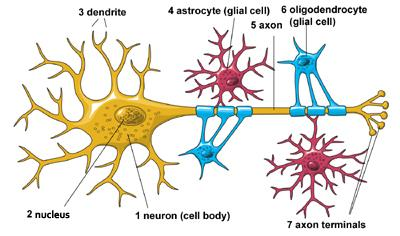
\includegraphics[width=0.65\textwidth]{imgs/NeuronArchitecture.jpg}
\caption{Neuron Architecture (Image taken from \href{https://www.ninds.nih.gov/}{National Institute of Neurological Disorders and Stroke, United States of America}, accessed on 20-May-2024).}\label{fig:neurons}
\end{figure}

\noindent Deep Learning Model များသည်  လူသားများ၏ အာရုံကြောစနစ်ရှိ neuron များ၏ အလုပ်လုပ်ပုံကို နမူနာယူ၍ တည်ဆောက်ထားခြင်းဖြစ်သည်။ neuron များသည် အချက်အလက်များကို ပို့ဆောင်ပေးခြင်း၊ သယ်ယူပေးခြင်းတာ၀န်ကို ထမ်းဆောင်သည့် messenger များဖြစ်ကြသည်။ 

neuron တစ်ခုတွင် ပြင်ပ (သို့မဟုတ်) အခြား neuron များမှ အချက်အလက် (signal) များကို ရယူမည့်  wire မျှင်များ (dendrites) ၊ ပြင်ပသို့ အချက်အလက်များ ပေးပို့မည့် Axon ဟု ခေါ်သည့် output wire များ နှင့် neuron ၏ အဓိက ခန္ဓာကိုယ် (cell body) ဟု အပိုင်း (၃) ပိုင်း ပါ၀င်သည် (Ref: Figure \ref{fig:neurons})။ dendrites မှတဆင့် ရလာသည့် အချက်အလက်များကို neuron ၏ အဓိက ခန္ဓာကိုယ် (cell body)မှ တွက်ချက်မှုများ ပြုလုပ်ပြီးနောက် ရလာသည့် ရလဒ်များကို Axon ဟု ခေါ်သည့် output wire များ မှ တဆင့် အခြား neuron များသို့ ပို့ပေးပါသည်။ထိုသို့ပေးပို့လာသည့် အချက်အလက် (signal) များကို အခြား neuron တစ်ခုမှ လက်ခံရယူပြီး အချက်အလက်များ ဆက်လက်ပို့ဆောင်ခြင်းများ ပြုလုပ်ကြပါသည်။ ထိုကဲ့သို့ neuron များ ချိတ်ဆက် အလုပ်လုပ်ခြင်းကို neural network ဟု ခေါ်ဆိုခြင်း ဖြစ်သည်။ 

လူသားများ၏ အာရုံကြောစနစ်ကို အခြေခံ၍ Artificial neural network architecture များကို Artificial neurons များစွာ ပါ၀င်သည့် layer များဖြင့် ချိတ်ဆက် ဖွဲ့စည်းထားသည်။ Layer တစ်ခုတွင် တစ်ခုထက်ပိုသော neuron များ ပါ၀င်ပြီး အဆိုပါ neuron များမှ အချက်အလက်ရယူခြင်း၊ တွက်ချက်ခြင်းနှင့် ရလဒ်များထုတ်ပေးခြင်းတို့ကို ထမ်းဆောင်ကြသည်။ neural network architecture တစ်ခုတွင် input layer ၊  တစ်ခုထက်ပိုသော hidden layer များ နှင့် ရလဒ် ထုတ်ပေးသည့် output layer (neuron) တို့ ပါ၀င်သည်။ 

\section{Neural Network Architecture} \label{sec:architecture}

Deep learning models excel at tackling complex problems by leveraging neural networks with multiple hidden layers. However, to lay a solid foundation, we begin with one-layer neural networks before moving onto multi-layer neural networks. 

\subsection{Single-Layer Neural Network}\label{sec:SLP}
The simplest form of a neural network is the one-layer neural network, also known as a single-layer perceptron. This basic building block helps in understanding the more complex architectures used in deep learning. A one-layer neural network consists of three main components:

\begin{itemize}
  \item Input Layer: Takes input features.
  \item Weights and Bias: Each input is assigned a weight, and a bias term is added.
  \item Activation Function: Computes the output of the neuron.
\end{itemize}

Deep Learning Model များသည် hidden layer များစွာပါ၀င်သော neural network architecture များ ဖြစ်သည်။ သို့သော် neural network ၏ အခြေခံ သဘောတရားကို နားလည်စေရန်အတွက် layer တစ်ခုသာ ပါ၀င်သော  one-layer neural network  မှ စ၍ ရှင်းပြသွားမည် ဖြစ်သည်။ One-layer neural network သည် အလွယ်ကူ အရိုးရှင်းဆုံးသော neural network တစ်ခု ဖြစ်ပြီး အစိတ်အပိုင်း (၃)ခု ပါ၀င်သည်။ 

\begin{itemize}
  \item Input Layer: Input layer တွင် ပါ၀င်သည့်  neuron တစ်ခုချင်းစီသည် Input feature တစ်ခုစီနှင့် တိုက်ရိုက်ချိတ်ဆက်ထားသည်။ 
  \item Weights and Bias: weight (မြှောက်ဖော်ကိန်း) များသည် Input feature တစ်ခုချင်းစီ၏ အရေးပါမှုကို ဆုံးဖြတ်ပေးသည်။ ထို့အပြင် Bias Unit တစ်ခုကိုလည်း ထည့်သွင်းစဥ်းစားရမည်။ 
  \item Activation Function: Activation Function သည် တွက်ချက်မှုများကို ပြုလုပ်ပြီး ရလဒ်ကို ရှာပေးမည့် Function ဖြစ်သည်။ 
\end{itemize}

\begin{figure}[h]%
\centering
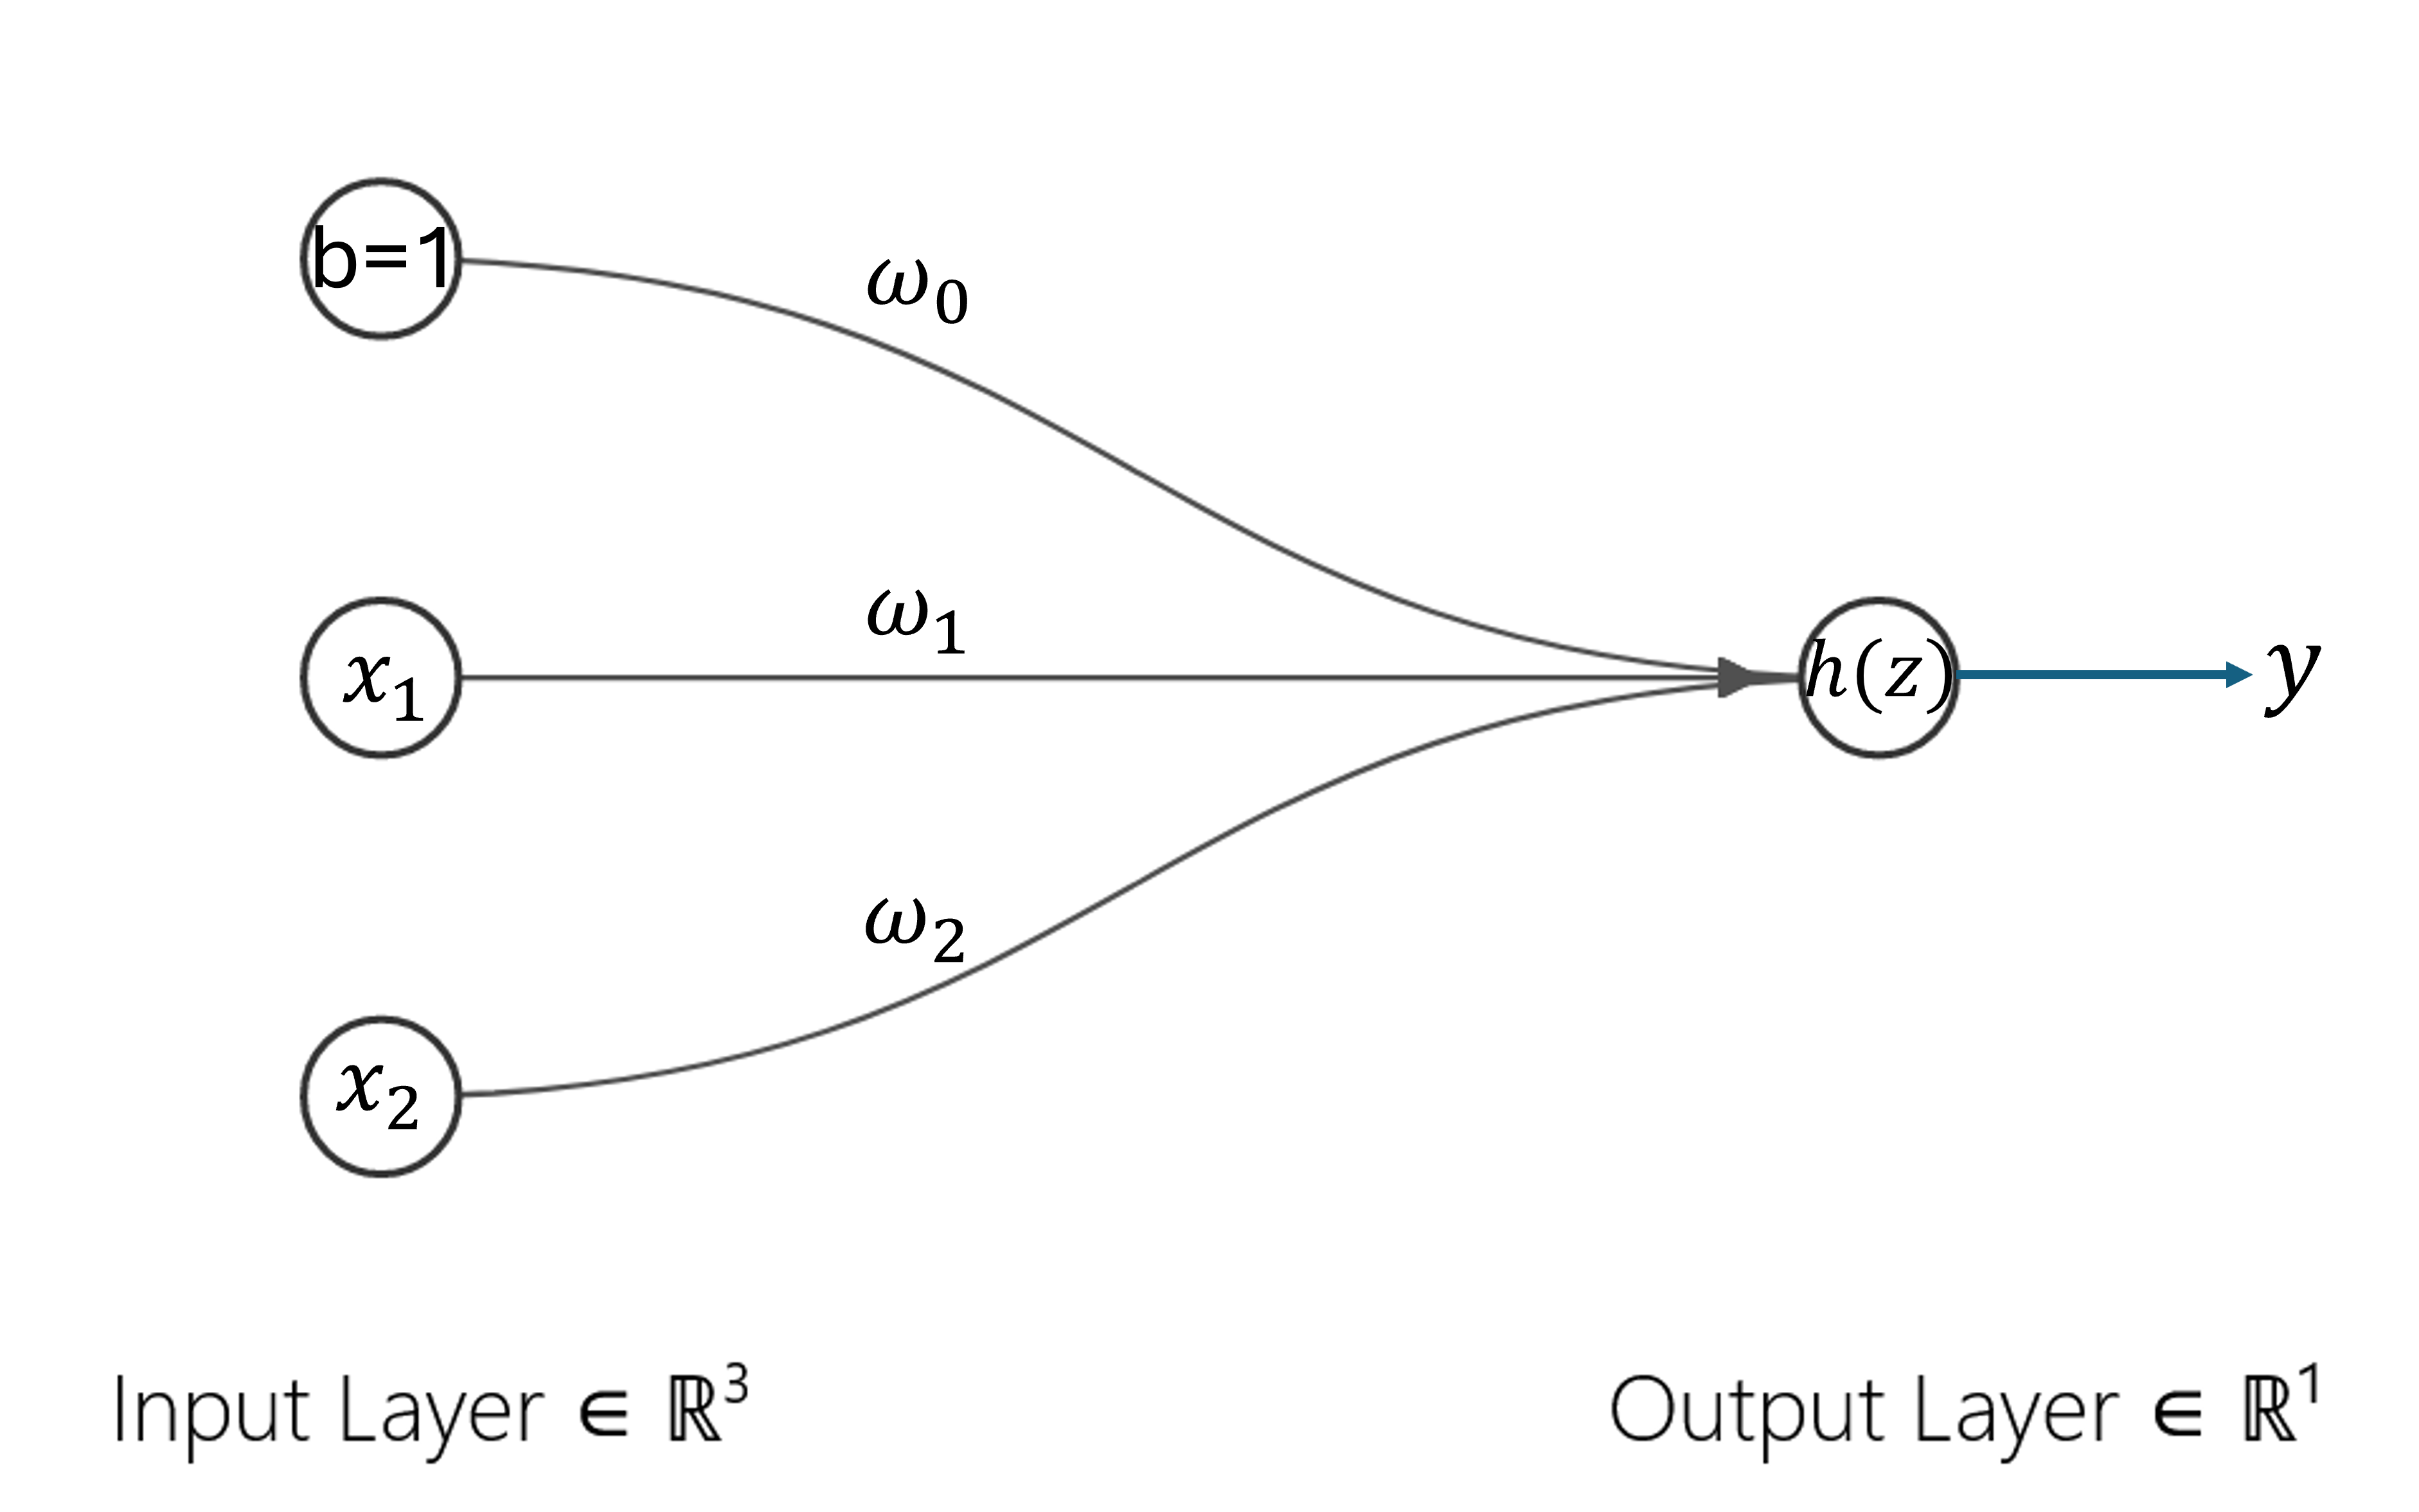
\includegraphics[width=0.675\textwidth]{imgs/slp.png}
\caption{Example of Single-Layer Perception (One Layer Neural Network) with two features. Image is generated using NN-SVG\cite{web:NNSVG}}\label{fig:slp}
\end{figure}

Figure \ref{fig:slp} illustrates a single-layer neural network with two input features. For example, suppose this network models the prediction of a company's sales amount based on TV and radio advertisement costs. The nodes $( x_1 ) $, $( x_2)$, represent these input features, while $( b = 1) $ serves as a bias unit. The bias unit $( b=1) $ is a constant added to the input to enhance model fitting. The weights $(\omega_1)$ and $(\omega_2)$ determine the importance of the associated features. The activation function $h(z)$ applies a transformation to the weighted sum of inputs and produces the output. During training, these weights are adjusted iteratively to minimize errors and ensure alignment between predicted and actual outputs.  

\noindent ဥပမာ - အထက်ပါပုံတွင် ပြသထားသည့် single-layer neural network သည် ကုမ္ပဏီတစ်ခု၏ ရောင်းအားကို ခန့်မှန်းပေးမည့် Machine Learning Model တစ်ခုဟု ဆိုကြပါစို့။  ကုမ္ပဏီ၏ ရောင်းအားကို TV နှင့် radio ကြော်ငြာခ အတွက် အသုံးပြုသည့် ကုန်ကျစရိတ်များကို မူတည်၍ ခန့်မှန်းမည်။ ဤဥပမာတွင် nodes $( x_1 ) $ နှင့် $( x_2)$ သည် TV နှင့် radio ကြော်ငြာခ များကို ကိုယ်စားပြုသည်။  

$( b = 1) $ သည် ကြော်ငြာခ လုံး၀ အသုံးမပြုသည့် အခြေအနေတွင် ဖြစ်ပေါ်နိုင်သည့် ရောင်းအားကို သိရှိနိုင်ရန် ထည့်ပေးသည့် ကိန်းသေတစ်ခုဖြစ်ပြီး bias unit ဟု ခေါ်သည်။ မြှောက်ဖော်ကိန်း $(\omega_1)$ နှင့် $(\omega_2)$ များသည် ရောင်းအားကို တွက်ချက်ရာတွင် TV နှင့် radio ကြော်ငြာခ တို့၏ အရေးပါမှုနှင့် တိုက်ရိုက်အချိုးကျသည်။ ဥပမာ - TV ကြော်ငြာခ တိုးလိုက်သည့် အချိန်တွင် ရရှိသည့် ရောင်းအား ပမာဏသည် radio ကြော်ငြာခ တိုးလိုက်သည့် အချိန်တွင် ရရှိသည့် ရောင်းအားပမာဏ ထက်များနေမည်ဆိုပါက $(\omega_1)$ ၏ တန်ဖိုးသည် $(\omega_2)$ ၏ တန်ဖိုးထက်များမည် ဖြစ်သည်။ 

Machine Learning Model တစ်ခုတည်ဆောက်သည် (သို့မဟုတ်) Train လုပ်သည် ဆိုသည်မှာ တနည်းအားဖြင့် အထက်ပါ မြှောက်ဖော်ကိန်း  $(\omega_1)$ နှင့် $(\omega_2)$ များ၏ တန်ဖိုးကို ရှာဖွေခြင်းပင် ဖြစ်သည်။ 

\subsection{Multi-layer Neural Network}\label{MLP}

A multi-layer neural network, specifically a Multi-Layer Perceptron (MLP), extends the concept of the single-layer perceptron by introducing one or more hidden layers between the input and output layers. This additional complexity allows the network to learn and represent more intricate patterns and relationships in the data, making it capable of solving more complex problems.

\noindent An MLP typically consists of three types of layers:
\begin{itemize}
  \item \textbf{Input Layer}: The layer that receives the input features.
  \item \textbf{Hidden Layers}: One or more intermediate layers where the computation happens. These layers perform transformations on the input data.
  \item \textbf{Output Layer}: The final layer that produces the output, such as class probabilities in classification tasks.
\end{itemize}

\begin{figure}[h]%
\centering
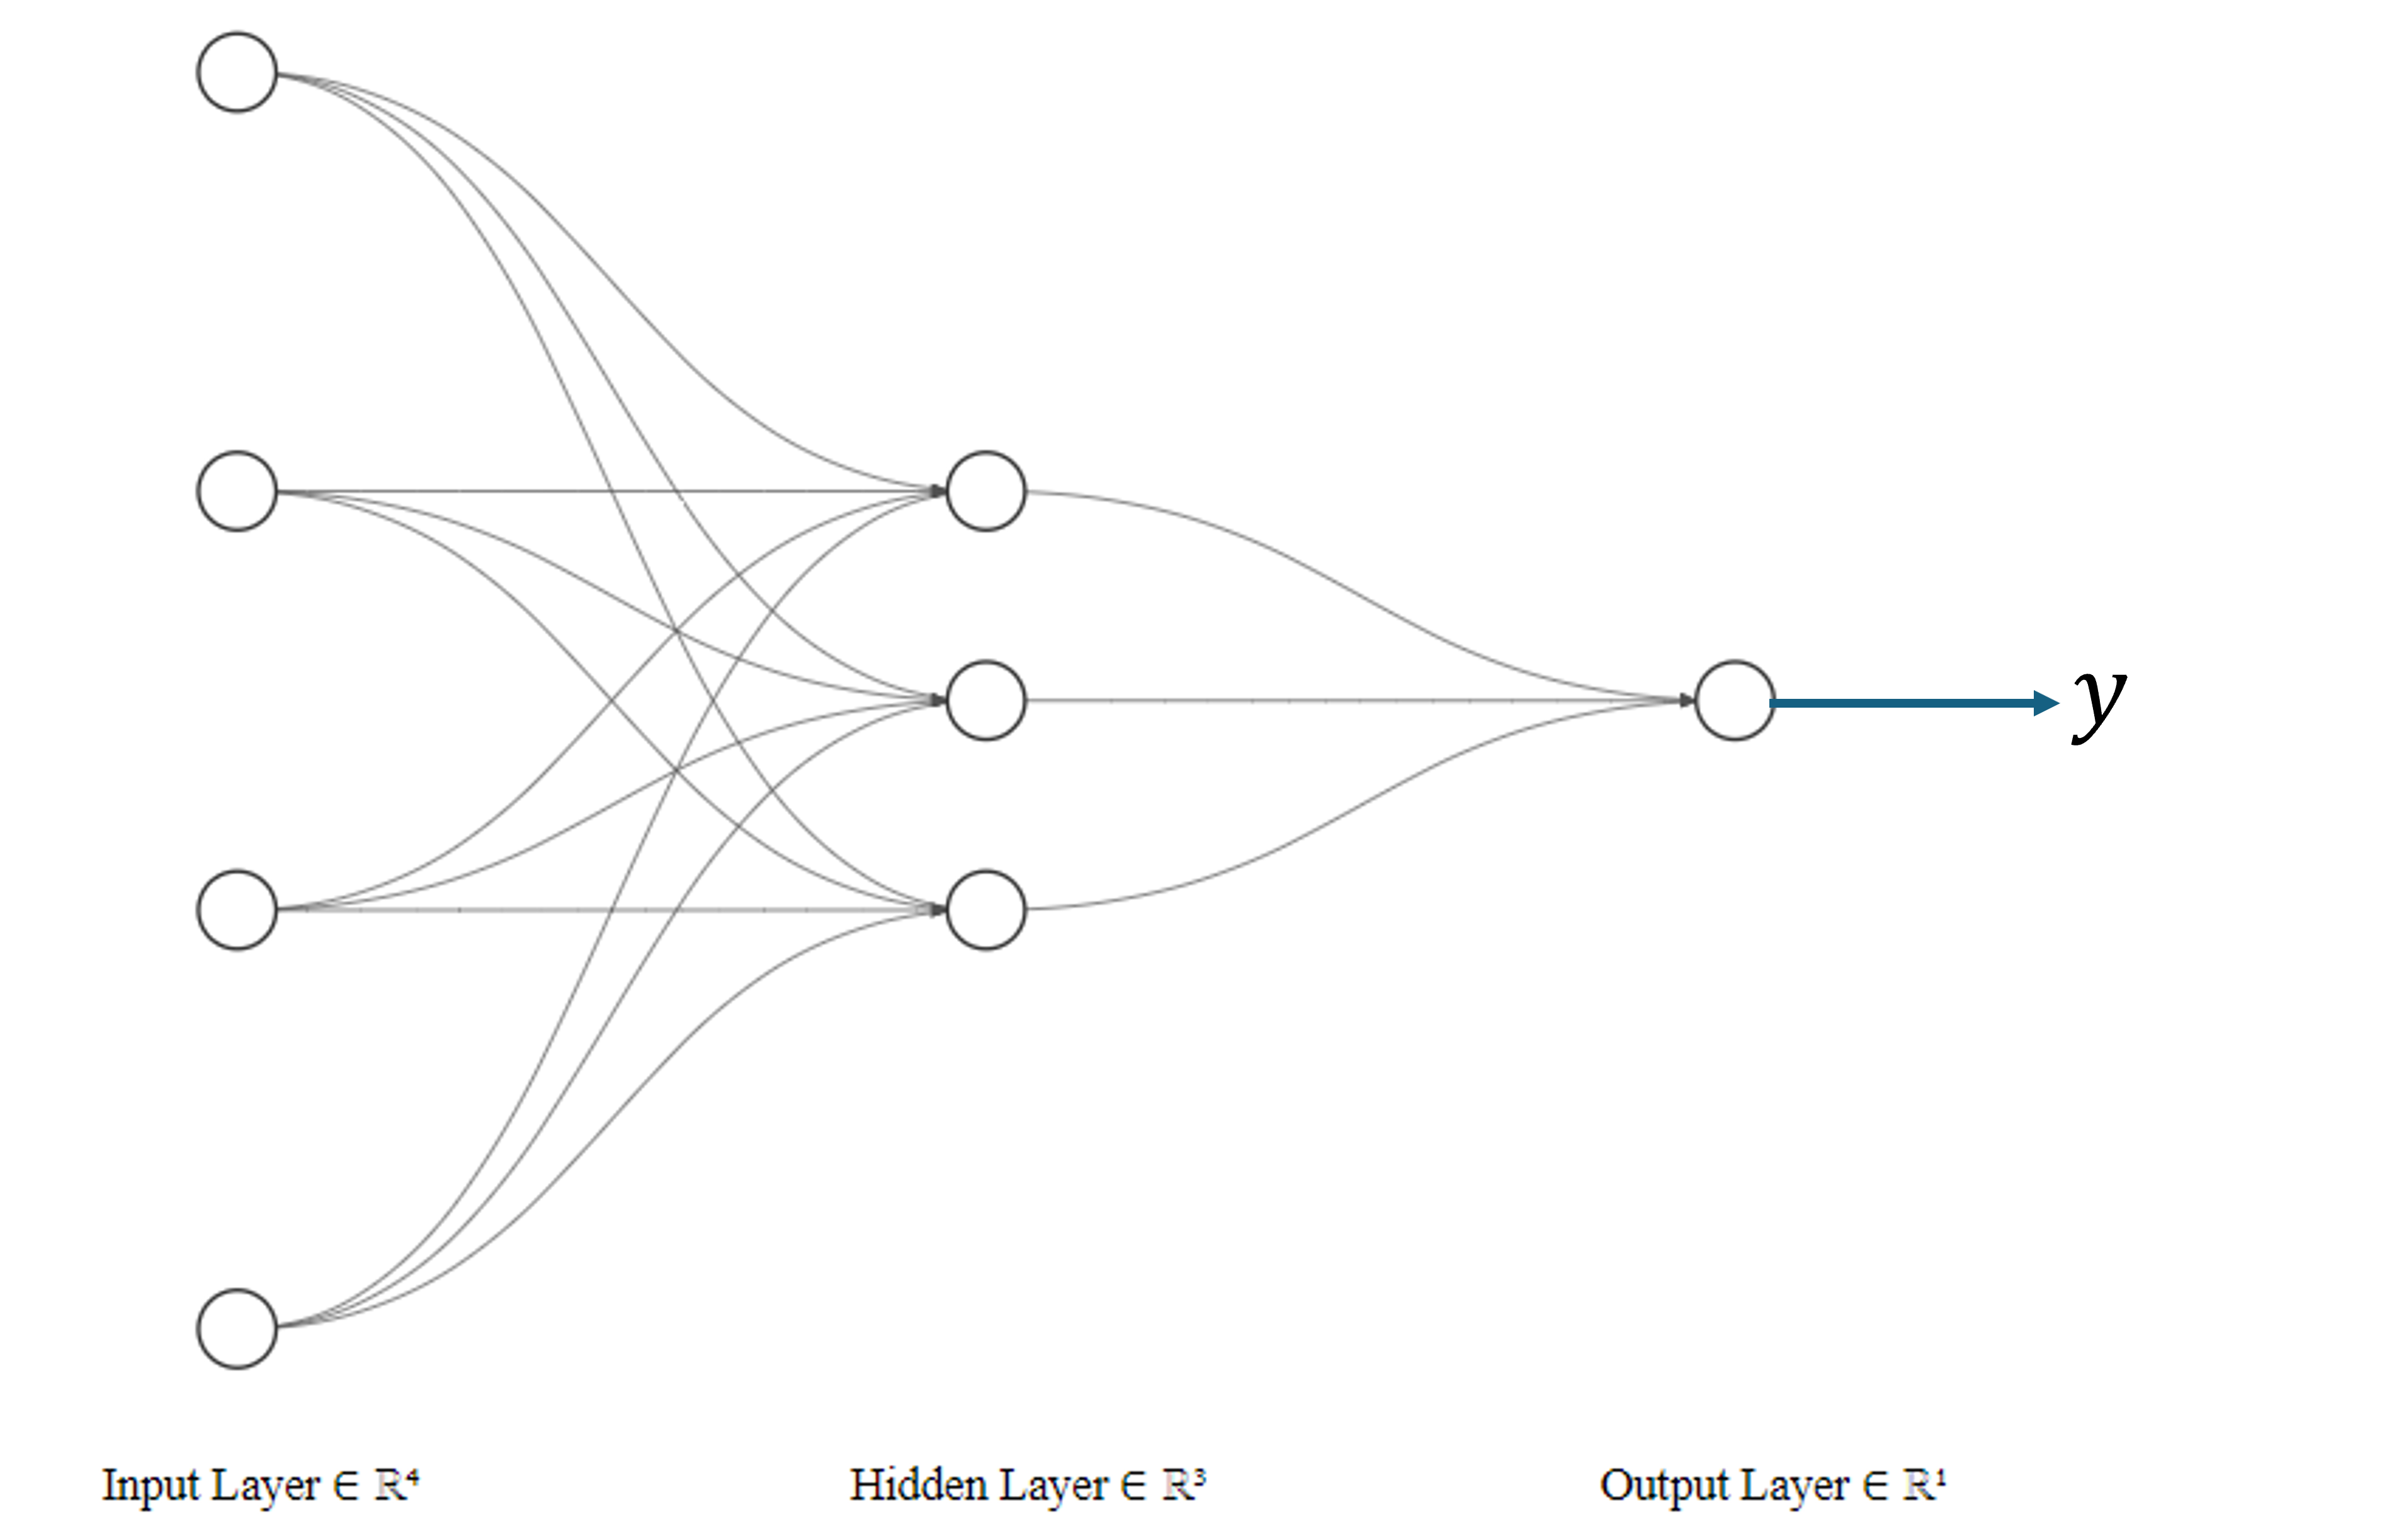
\includegraphics[width=0.7\textwidth]{imgs/mlp.png}
\caption{Example of Multi-Layer Perception with one hidden lyaer. Image is generated using NN-SVG\cite{web:NNSVG}}\label{fig:mlp}
\end{figure}

\vspace{0.25em}
\noindent Multi-layer neural network အထူးသဖြင့် Multi-Layer Perceptron သည်  single-layer perceptron (သို့) neural network တွင် hidden layer များထည့်ထားခြင်း ဖြစ်သည်။ Multi-Layer Perceptron တစ်ခုတွင် 

\begin{itemize}
  \item \textbf{Input Layer}: Input layer တွင် ပါ၀င်သည့်  neuron တစ်ခုချင်းစီသည် Input feature တစ်ခုစီနှင့် တိုက်ရိုက်ချိတ်ဆက်ထားသည်။ 
  \item \textbf{Hidden Layers}: ကြားခံ layer များဖြစ်ပြီး ၄င်း layer များသည် Input feature များကို အဆင့်ဆင့် ပြောင်းလဲ ပေးသွားသည်။ 
  \item \textbf{Output Layer}: Neural network ၏ နောက်ဆုံး layer ဖြစ်ပြီး output ကို ထုတ်ပေးသည်။ 
\end{itemize}

\subsection{Deep Learning Architecture}\label{deepNN}

The term \texttt{``deep learning"} refers to neural networks with multiple layers between the input and output layers \cite{Goodfellow-et-al-2016}. While traditional neural networks (often called shallow networks discussed in the previous chapter) typically have one or two hidden layers, deep learning networks usually have many more—sometimes reaching dozens or even hundreds of layers. This increased depth enables the network to learn hierarchical representations of data, capturing intricate features at various levels of abstraction \cite{lecun2015deep}.

A defining feature of deep learning is its ability to autonomously learn representations from raw data. Each subsequent layer in a deep network learns increasingly abstract features from the preceding one. For instance, when a deep neural network tries to classify an image, the initial hidden layers build up patterns or interactions that are conceptually simple. These initial layers look at groups of nearby pixels to find patterns like diagonal lines, horizontal lines, vertical lines, and areas of blur by examining groups of nearby pixels. As the network progresses through the layers, subsequent layers combine that information to detect larger patterns, such as squares or circles. Later layers put together these larger shapes to recognize complex structures like a checkerboard pattern, a face, or a car. 

The advantage of deep learning lies in its capacity to automatically acquire hierarchical features from data, facilitating precise identification and classification of objects in images. However, this prowess comes at a cost—deep networks necessitate substantial computational resources and large amounts of labeled data for effective training. Nonetheless, advancements in hardware, particularly Graphics Processing Units (GPUs), coupled with innovative algorithms, have rendered the training of these deep networks feasible.

Common deep learning architectures include Convolutional Neural Networks (CNNs) for image data, Recurrent Neural Networks (RNNs) and Long Short-Term Memory networks (LSTMs) for sequential data, and Transformer models for natural language processing. 

\vspace{0.5em}
\noindent Deep Learning သည် input နှင့် output layer အကြား layer များစွာ ပါ၀င်သည့် neural network model များ ဖြစ်သည်။ ပြီးခဲ့သည့် အခန်းတွင် ဆွေးနွေးခဲ့သည့် neural network model များတွင် hidden layer တစ်ခု (သို့မဟုတ်) နှစ်ခုသာ ပါ၀င်ကြပြီး ၄င်းတို့ကို \texttt{shallow} network များဟုလည်း ခေါ်ဆိုကြသည်။ Deep Learning model များတွင်မူ layer များစွာ ပါ၀င်ပြီး တစ်ခုနှင့် တစ်ခုအကြား ဒေတာများ၏ ချိတ်ဆက်မှုကို အဆင့်ဆင့် အလိုအလျောက် လေ့လာနိုင်သည်။ 

ဥပမာ - face image များကို အသုံးပြု၍  ဖုန်း authorize ပြုလုပ်မည့် deep learning model တစ်ခုတွင် Input Layer ၌ ပေးလိုက်သည့် ဒေတာများသည် image ရှိ pixel တစ်ခုချင်းစီ၏ intensity တန်ဖိုးများ ဆိုပါစို့။ အဆိုပါ  intensity များ၏ ချိတ်ဆက်မှုကို လေ့လာခြင်းဖြင့် ဒုတိယ Layer တွင် intensity တန်ဖိုးတူသည့် အုပ်စုများကို စုဖွဲ့ခြင်း၊ ရုတ်တရက် ပြောင်းလဲသွားသည့် pixel များကို ချိတ်ဆက်ခြင်းဖြင့် ဓါတ်ပုံတွင် ပါ၀င်သော မျက်နှာ၏ edge ကို detect လုပ်သွားနိုင်သည်။ ထိုမှတဆင့် အဆင့်ဆင့် Layer များတွင် မျက်နှာပြင်၏ ထူးခြားသည့် လက္ခဏာများကို ချိတ်ဆက် ပုံဖော်ခြင်းဖြင့် နောက်ဆုံးအဆင့်တွင် face image တွင် ပါ၀င်သည့် လူသည် authorize ပြုလုပ်သင့်သည့် ဟုတ်/မဟုတ်ကို မှန်မှန်ကန်ကန် ခန့်မှန်းနိုင်သည်။ 

\noindent သို့သော် ထိုကဲ့သို့ Layer များစွာ ပါ၀င်သည့် Deep Learning model တစ်ခုကို တည်ဆောက်နိုင်ရန်အတွက် အချက်အလက်များစွာ လိုအပ်သကဲ့သို့ computational power မြင့်မားသည့် ကွန်ပြူတာများ၊ ဆာဗာများလိုအပ်သည်။  GPU, or Graphics Processing Unit များထွက်ပေါ်လာခြင်းသည် Deep Learning model များ တည်ဆောက်ရန်အတွက် များစွာ အထောက်အကူ ဖြစ်စေသည်။ 

\noindent ယနေ့ခတ်တွင် လူသုံးများသည့် deep learning architecture များမှာ 
\begin{itemize}
  \item ဓါတ်ပုံ ၊ image ဒေတာများအတွက်  Convolutional Neural Networks (CNNs) ၊ 
  \item စာသား ၊ အသံစသည့် sequential ဒေတာများ အတွက် Recurrent Neural Networks (RNNs) နှင့် 
  \item Transformer model များဖြစ်ကြသည်။ 
\end{itemize}

\newpage 
\section{Activation Functions}\label{sec:activation}

The activation function $h(z)$ computes the final output of the neuron based on its pre-activation value. For a single neuron  in the neural network layer shown in Figure \ref{fig:slp}, the pre-activation value $z$ represents the weighted sum of inputs to a neuron, including the bias term.

\begin{equation}\label{eqn:hz}
  z = \omega_1 x_1 + \omega_2 x_2 + \omega_0, 
\end{equation} where 

\begin{itemize}[b]
  \item $(\omega_1)$ and $(\omega_2)$ are the weights associated with the connections from input features to the output neuron. 
  \item $( x_1 ) $, and $( x_2)$, are the input features (e.g., TV and radio advertisement costs).
  \item $b=1$ is the bias term associated with the output neuron.
\end{itemize}

\noindent In general, the equation \ref{eqn:hz} is written as: 
\begin{equation}\label{eqn:hz2}
  z = \sum_{i=1}^{n} \omega_i x_i + \omega_0, 
\end{equation} where $n$ is the number of features. 

\vspace{0.5em}
Common activation functions include Step, Sigmoid, ReLU (Rectified Linear Unit),  and Hyperbolic Tangent (tanh) Function. The choice of activation function depends on the specific task and the characteristics of the data. Experimentation with different activation functions is common to find the one that yields the best performance for a given problem.

\vspace{0.5em}
\noindent အထက်ပါပုံ  \ref{fig:slp} တွင် ပြသထားသည့် single-layer neural networkတွင် pre-activation value, $z$ ၏ တန်ဖိုးသည် မြှောက်ဖော်ကိန်းများနှင့် မြှောက်ထားသည့် ကြော်ငြာခ - ၂ ခု ၏ ပေါင်းခြင်းနှင့် ညီမျှသည် (ညီမျှခြင်း \ref{eqn:hz} ကို ကြည့်ပါ)။  ဤဥပမာတွင် input feature ၂ ခုသာပါ၀င်ပြီး $( x_1 ) $ နှင့် $( x_2)$ သည် TV နှင့် radio ကြော်ငြာခ များကို ကိုယ်စားပြုသည်။ input feature များစွာ ပါ၀င်သော ပုစ္ဆာအတွက် ဆိုပါက ညီမျှခြင်း \ref{eqn:hz2} ကို အသုံးပြုရမည်။ တနည်းဆိုသော် pre-activation value, $z$ သည် မြှောက်ဖော်ကိန်းများနှင့် မြှောက်ထားသည့် input feature များ၏ စုစုပေါင်းတန်ဖိုး ဖြစ်သည်။

\noindent Activation function အမျိုးမျိုးရှိပြီး လူသုံးများသည့် function များမှာ Step၊ Sigmoid၊  ReLU (Rectified Linear Unit) နှင့် Hyperbolic Tangent (tanh) Function တို့ဖြစ်ကြသည်။ ပုစ္ဆာ၏ သဘောတရားနှင့် ဒေတာ အမျိုးအစားများအပေါ်မူတည်၍ Activation function ကို ရွေးချယ်ကြလေ့ ရှိသည်။ 

\subsection{Step Function}\label{sec:activation}
This function produces binary output, typically 0 or 1, based on whether the input exceeds a certain threshold, $\theta$. It's commonly used for binary classification tasks. The mathematical representation of the step function, $h_{step}(z)$ is 
      \begin{equation}\label{eqn:step}
            h_{\text{step}}(z) = 
                                        \begin{cases}
                                        1, & \text{if } z \geq \theta \\
                                        0, & \text{otherwise}
                                        \end{cases}
    \end{equation} where $\theta$ is the threshold value. 
    
\begin{figure}[h]%
\centering
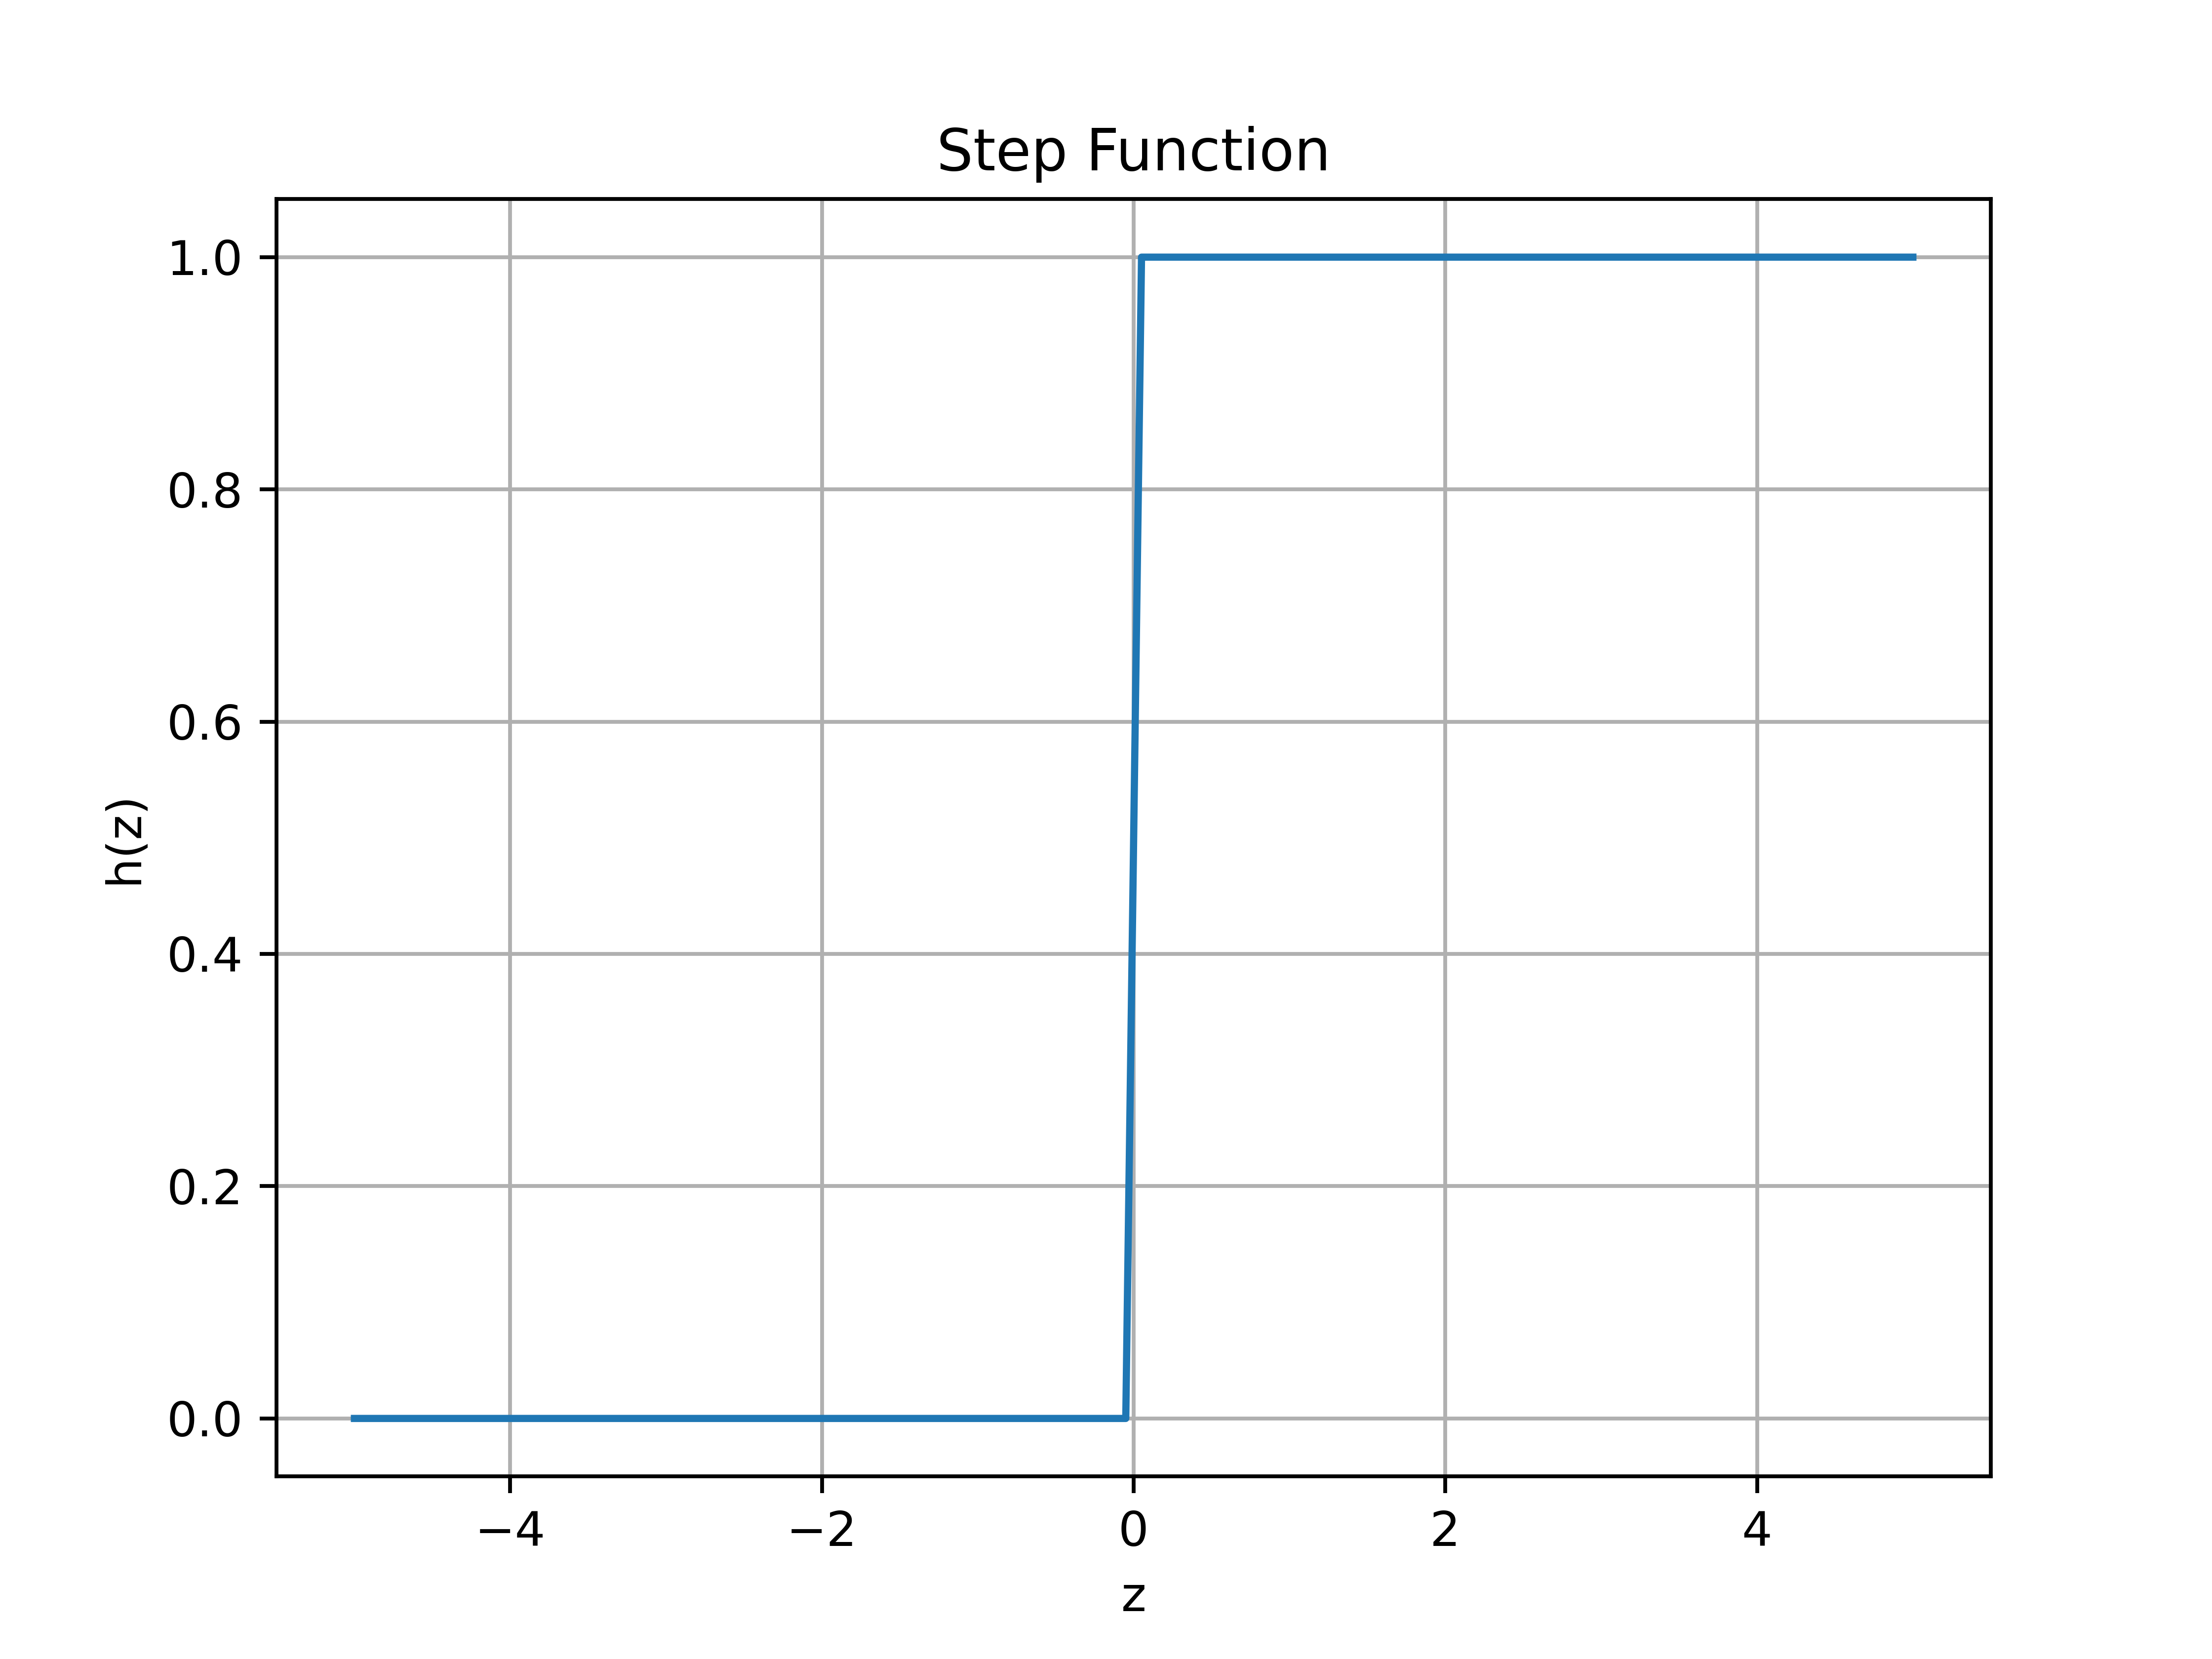
\includegraphics[width=0.6\textwidth]{imgs/step_fun.png}
\caption{Illustration of Step Function. Image is generated using Python.}\label{fig:step}
\end{figure}

Figure \ref{fig:step} illustrates a step function. As can be seen, the x-axis represents the pre-activation value $z$, and the y-axis represents the output of the function. It produces a binary value of 0 for all inputs below the threshold and 1 for all inputs above the threshold. The step activation function was historically used in early neural networks. However, it is rarely used in modern deep learning due to its binary nature.

\vspace{0.5em} 
Step Function ကို Binary classification ပုစ္ဆာများအတွက် အဓိက အသုံးပြုခဲ့ကြသည်။ Binary classification ပုစ္ဆာ နမူနာ အချို့မှာ - စာမေးပွဲ အအောင်၊ အရှုံး သတ်မှတ်ခြင်း၊ ပန်းသီး တစ်လုံး အပုတ်၊ အကောင်း ဆုံးဖြတ်ခြင်း စသည်တို့ ဖြစ်သည်။ ရလဒ်မှာ 'အောင်သည်' (သို့မဟုတ်) 'ကျသည်' - အဖြေ ၂ ခု အနက် - တစ်ခုသာ ဖြစ်သည်။ ပုံ  \ref{fig:step} တွင် Step Function ၏ သဘောတရားကို ဖော်ပြထားသည်။ အကယ်၍ pre-activation value $z$ ၏ တန်ဖိုးသည် ကြိုတင်သတ်မှတ်ထားသည့် ကိန်းသေ (threshold) ထက် နည်းပါက ရလဒ် - သုည (`ကျသည်') ကို ထုတ်ပေးပြီး ကိန်းသေ (threshold) ထက် များပါက ရလဒ် - တစ် (`အောင်သည်') ဟု ထုတ်ပေးမည် ဖြစ်သည်။ 

Step Function ကို ယနေ့ခတ်တွင် မသုံးသလောက် နည်းပါးသွားပြီဖြစ်သည်။ ဤ Function ၏ ပြဿနာမှာ ကိန်းသေ (threshold) ၏ နေရာတွင် သုညမှ တစ်သို့ ရုတ်တရက် ပြောင်းလဲသွားခြင်း ဖြစ်သည်။  ဥပမာ - စာမေးပွဲ အအောင် ၊ အရှုံး ပြဿနာတွင် - အောင်မှတ် (threshold) ကို ၄၀ ဟုတ် သတ်မှတ်ထားပါက ၄၀.၁ မှတ် ရသော ကျောင်းသားသည် အောင်သော်လည်း ၃၉.၉ မှတ်ရသော ကျောင်းသားသည် ကျမည် ဖြစ်သည်။ 

\subsection{Sigmoid Function}
The sigmoid function is often used in the output layer for problems where the output needs to be probabilistic or numerical. It squashes the input values to the range between 0 and 1, which can be interpreted as probabilities. For instance, in a binary classification problem, the output of the sigmoid function can represent the probability of belonging to one of the two classes. If the probability is above a certain threshold (e.g., 0.5), the input is classified into one class; otherwise, it's classified into the other class. Mathematically, it is represented as: 

\begin{equation}\label{eqn:sigmoid}
    h_{sigmoid}(z) = \frac{1}{1 + exp(-z)}
\end{equation} where pre-activation value, $z$ is the input to the function, typically the weighted sum of the inputs plus a bias term. 

\begin{figure}[h]%
\centering
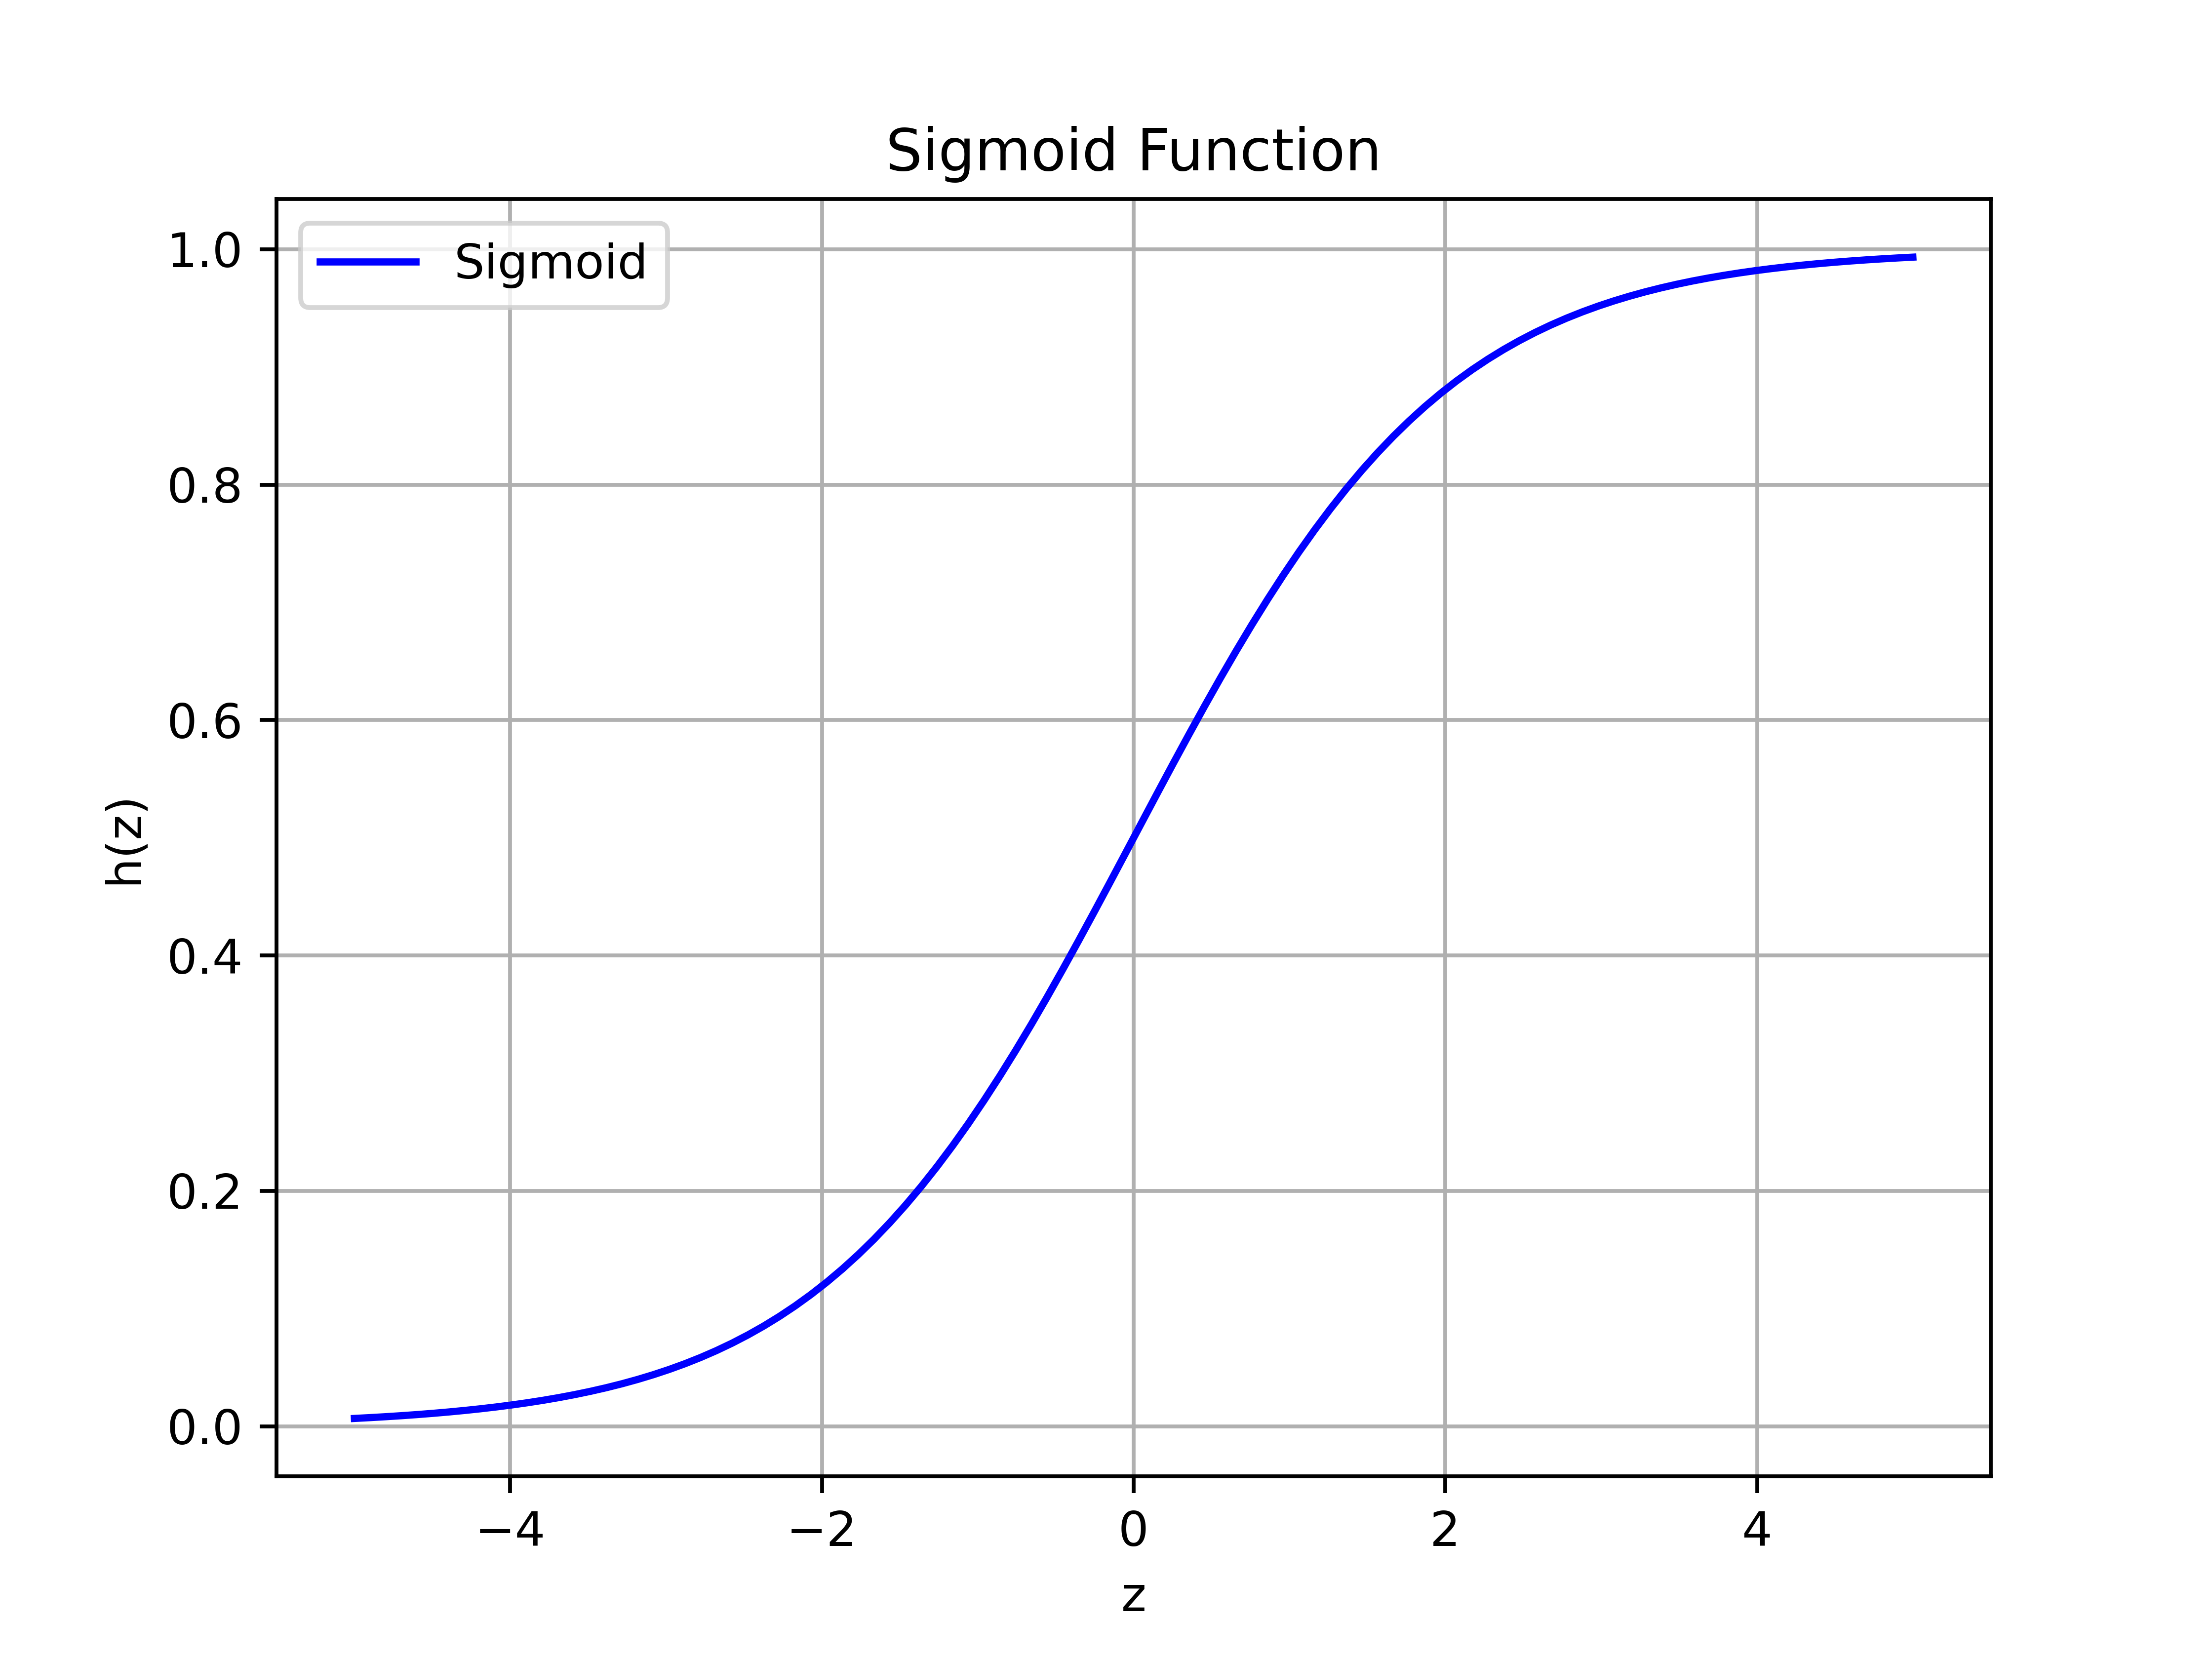
\includegraphics[width=0.55\textwidth]{imgs/sigmoid_fun.png}
\caption{Illustration of Sigmoid Function. Image is generated using Python.}\label{fig:sigmoid}
\end{figure}

As shown in Figure \ref{fig:sigmoid}, the sigmoid function is smooth and differentiable, which makes it suitable for gradient-based optimization techniques. However, one drawback is that it can cause the vanishing gradient problem in deep networks, where gradients become very small, slowing down or even preventing the network from training effectively. Despite this, the sigmoid function remains a popular choice for binary classification problems due to its probabilistic interpretation.

\vspace{1.5em} 

Sigmoid Function ကို Neural Network ၏ output layer အတွက် အသုံးပြုသည်။ ပုံ (\ref{fig:sigmoid}) တွင်ပြသထားသည့်အတိုင်း Sigmoid Function ၏ output သည် သုညမှ တစ် အတွင်းရှိပြီး probabilities တန်ဖိုးဟု ယူဆနိုင်သည်။ ဥပမာ - စာမေးပွဲ အအောင်၊ အရှုံး တွက်ချက်သည့် ပုစ္ဆာအတွက် Sigmoid Function သည် ကျောင်းသား၏ အောင်နိုင်ချေ ရာခိုင်နှုန်းကို တွက်ချက်ပေးသည်။ အကယ်၍ ကျောင်းသား (သို့မဟုတ်) ကျောင်းသူ ၏ pre-activation value $z$ သည် သုညထက်နည်းပါက Sigmoid Function ၏ တန်ဖိုးသည် ၀.၅ (သို့မဟုတ်) ၅၀ ရာခိုင်နှုန်းအောက် ဖြစ်မည် (ညီမျှခြင်း - \ref{eqn:sigmoid} ကို ကြည့်ပါ)။ 

ပုံ (\ref{fig:sigmoid}) တွင် မြင်ရသည့် အတိုင်း sigmoid function မှပေးသောရလဒ်သည် Step Function ကဲ့သို့ ရုတ်တရက် ပြောင်းလဲသွားခြင်းမျိုး မဟုတ်ဘဲ  ဖြည်းဖြည်းချင်း ပြောင်းလဲ သွားသည်။ pre-activation value $z$ ၏ တန်ဖိုအနည်း အများပေါ်မူတည်၍  sigmoid function ၏ ရလဒ်သည် သုည (သို့မဟုတ်) တစ် သို့ ဖြည်းဖြည်းချင်း ချဥ်းကပ်သွားသည်။ အဆိုပါ အားသာချက်ကြောင့် sigmoid function ကို Binary classification ပုစ္ဆာများအတွက် ယနေ့တိုင် အသုံးပြုနေဆဲ ဖြစ်သည်။ 

\subsection{Softmax Function} 

The Softmax function is an activation function commonly used in the output layer of neural networks for multi-class classification tasks. It transforms a vector of raw scores (logits) into a probability distribution, where each class's probability is proportional to the exponential of the logit for that class. The Softmax function ensures that the sum of the probabilities for all classes equals 1, making it possible to interpret the outputs as probabilities. The function is defined as:

\begin{equation}\label{eqn:softmax}
    h_{softmax}(z_i) = \frac{exp(z_i)}{\sum_{j=1}^{K}exp(z_j)}
\end{equation} where $z_i$ are the input logits for each class, $i$ and $K$ is the number of classes. 

\vspace{0.5em} 

\begin{figure}[h]%
\centering
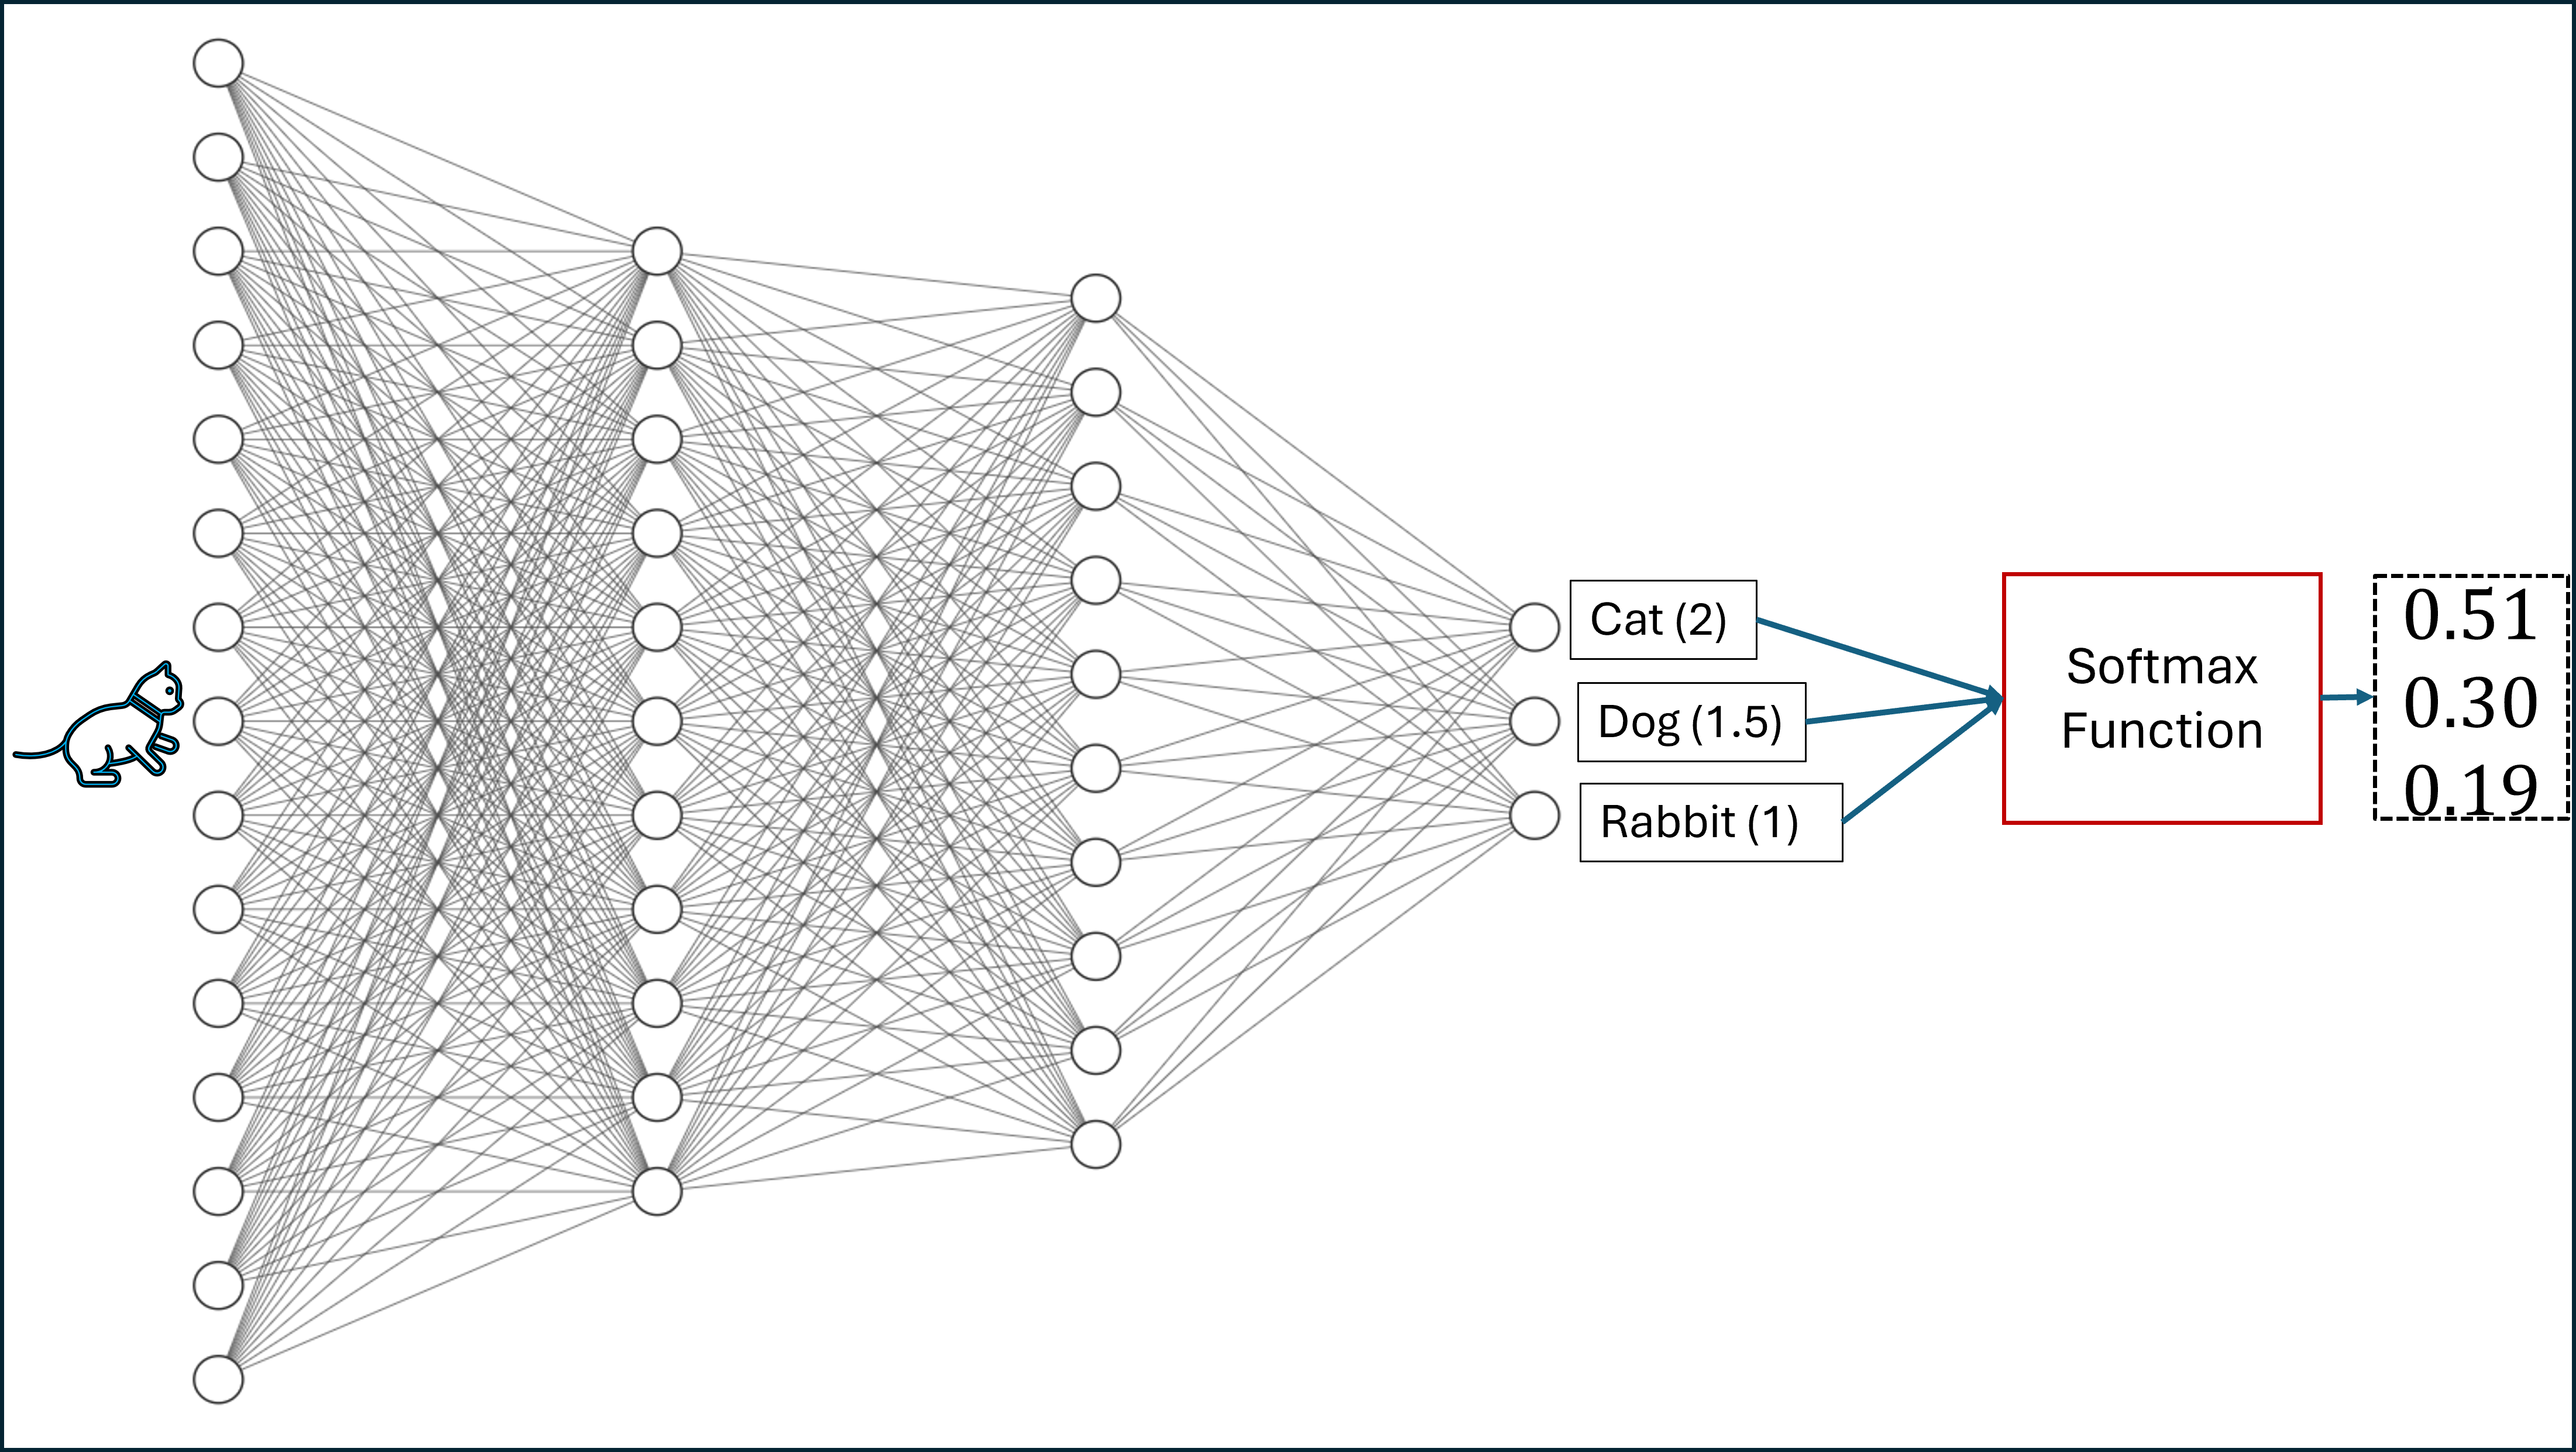
\includegraphics[width=0.65\textwidth]{imgs/softmax.png}
\caption{Illustration of Softmax Function for Multi-class Classification example. The neural network image was generated using NN-SVG \cite{web:NNSVG}.}\label{fig:softmax}
\end{figure}

Figure \ref{fig:softmax} shows an example of a neural network designed to classify images of animals into three categories: cats, dogs, and rabbits. When an image is fed into the neural network, the output layer provides raw scores (logits) for each class. Suppose the logits for a given image are 2 for cats, 1.5 for dogs, and 1 for rabbits. After applying the Softmax function (see Equation \ref{eqn:softmax}), the probabilities for each class are 0.51 (51\%), 0.30 (30\%), and 0.19 (19\%) respectively.

These probabilities sum to 1, making it possible to interpret them as the likelihood of the image belonging to each class. In this example, the neural network predicts that the image is most likely a cat with a 51\% probability.

\vspace{0.5em} 
\noindent Softmax function ကို Multi-Class Classification ပုစ္ဆာများအတွက် တည်ဆောက်သော Neural Network ၏ output layer တွင် အသုံးပြုသည်။ ၄င်း function သည် output layer မှ ရရှိသော အကြမ်း ရလဒ်များကို probability တန်ဖိုးများ အဖြစ် ပြောင်းပေးသည်။ 

ဥပမာ -- ဓါတ်ပုံတစ်ပုံကို ကြောင်၊ ခွေး နှင့် ယုန် အဖြစ် အမျိုးအစား ခွဲခြားပေးမည့် Neural Network တစ်ခုကို တည်ဆောက်ကြသည် ဆိုပါစို့။ Neural Network ၏ output layer မှ  တိရစ္ဆာန် အမျိုးအစား တစ်ခုချင်းစီအတွက် ရလဒ် အမှတ်များ ထုတ်ပေးသည်။ ထို့နောက် ပုံ \ref{eqn:softmax} တွင် ပြသထားသည့်အတိုင်း Softmax function မှ အဆိုပါ ရမှတ်များကို  probability တန်ဖိုးများ အဖြစ် ပြောင်းပေးသည်။ ရာခိုင်နှုန်းများ၏ ပေါင်းခြင်းမှာ တစ် ဖြစ်ပြီး ယခု ပုစ္ဆာတွင် ပေးထားသည့် ဓါတ်ပုံ သည် ကြောင်ဖြစ်နိုင်ချေ ၅၁ ရာခိုင်နှုန်း ၊ ခွေးဖြစ်နိုင်ချေ ၃၀ ရာခိုင်နှုန်းနှင့် ယုန်ဖြစ်နိုင်ချေ ၁၉ ရာခိုင်နှုန်း ရှိသည်။ 


\subsection{ReLU (Rectified Linear Unit) Function}
The ReLU function, as illustrated in Figure \ref{fig:relu}, returns the input if it's positive, otherwise, it returns zero. It's widely used in hidden layers of neural networks and has been found to accelerate convergence during training. Mathematically, 

\begin{equation}\label{eqn:relu}
    h_{ReLu}(z) = \max(0, z)
\end{equation} where $z$ is the pre-activation value. 

\begin{figure}[h]%
\centering
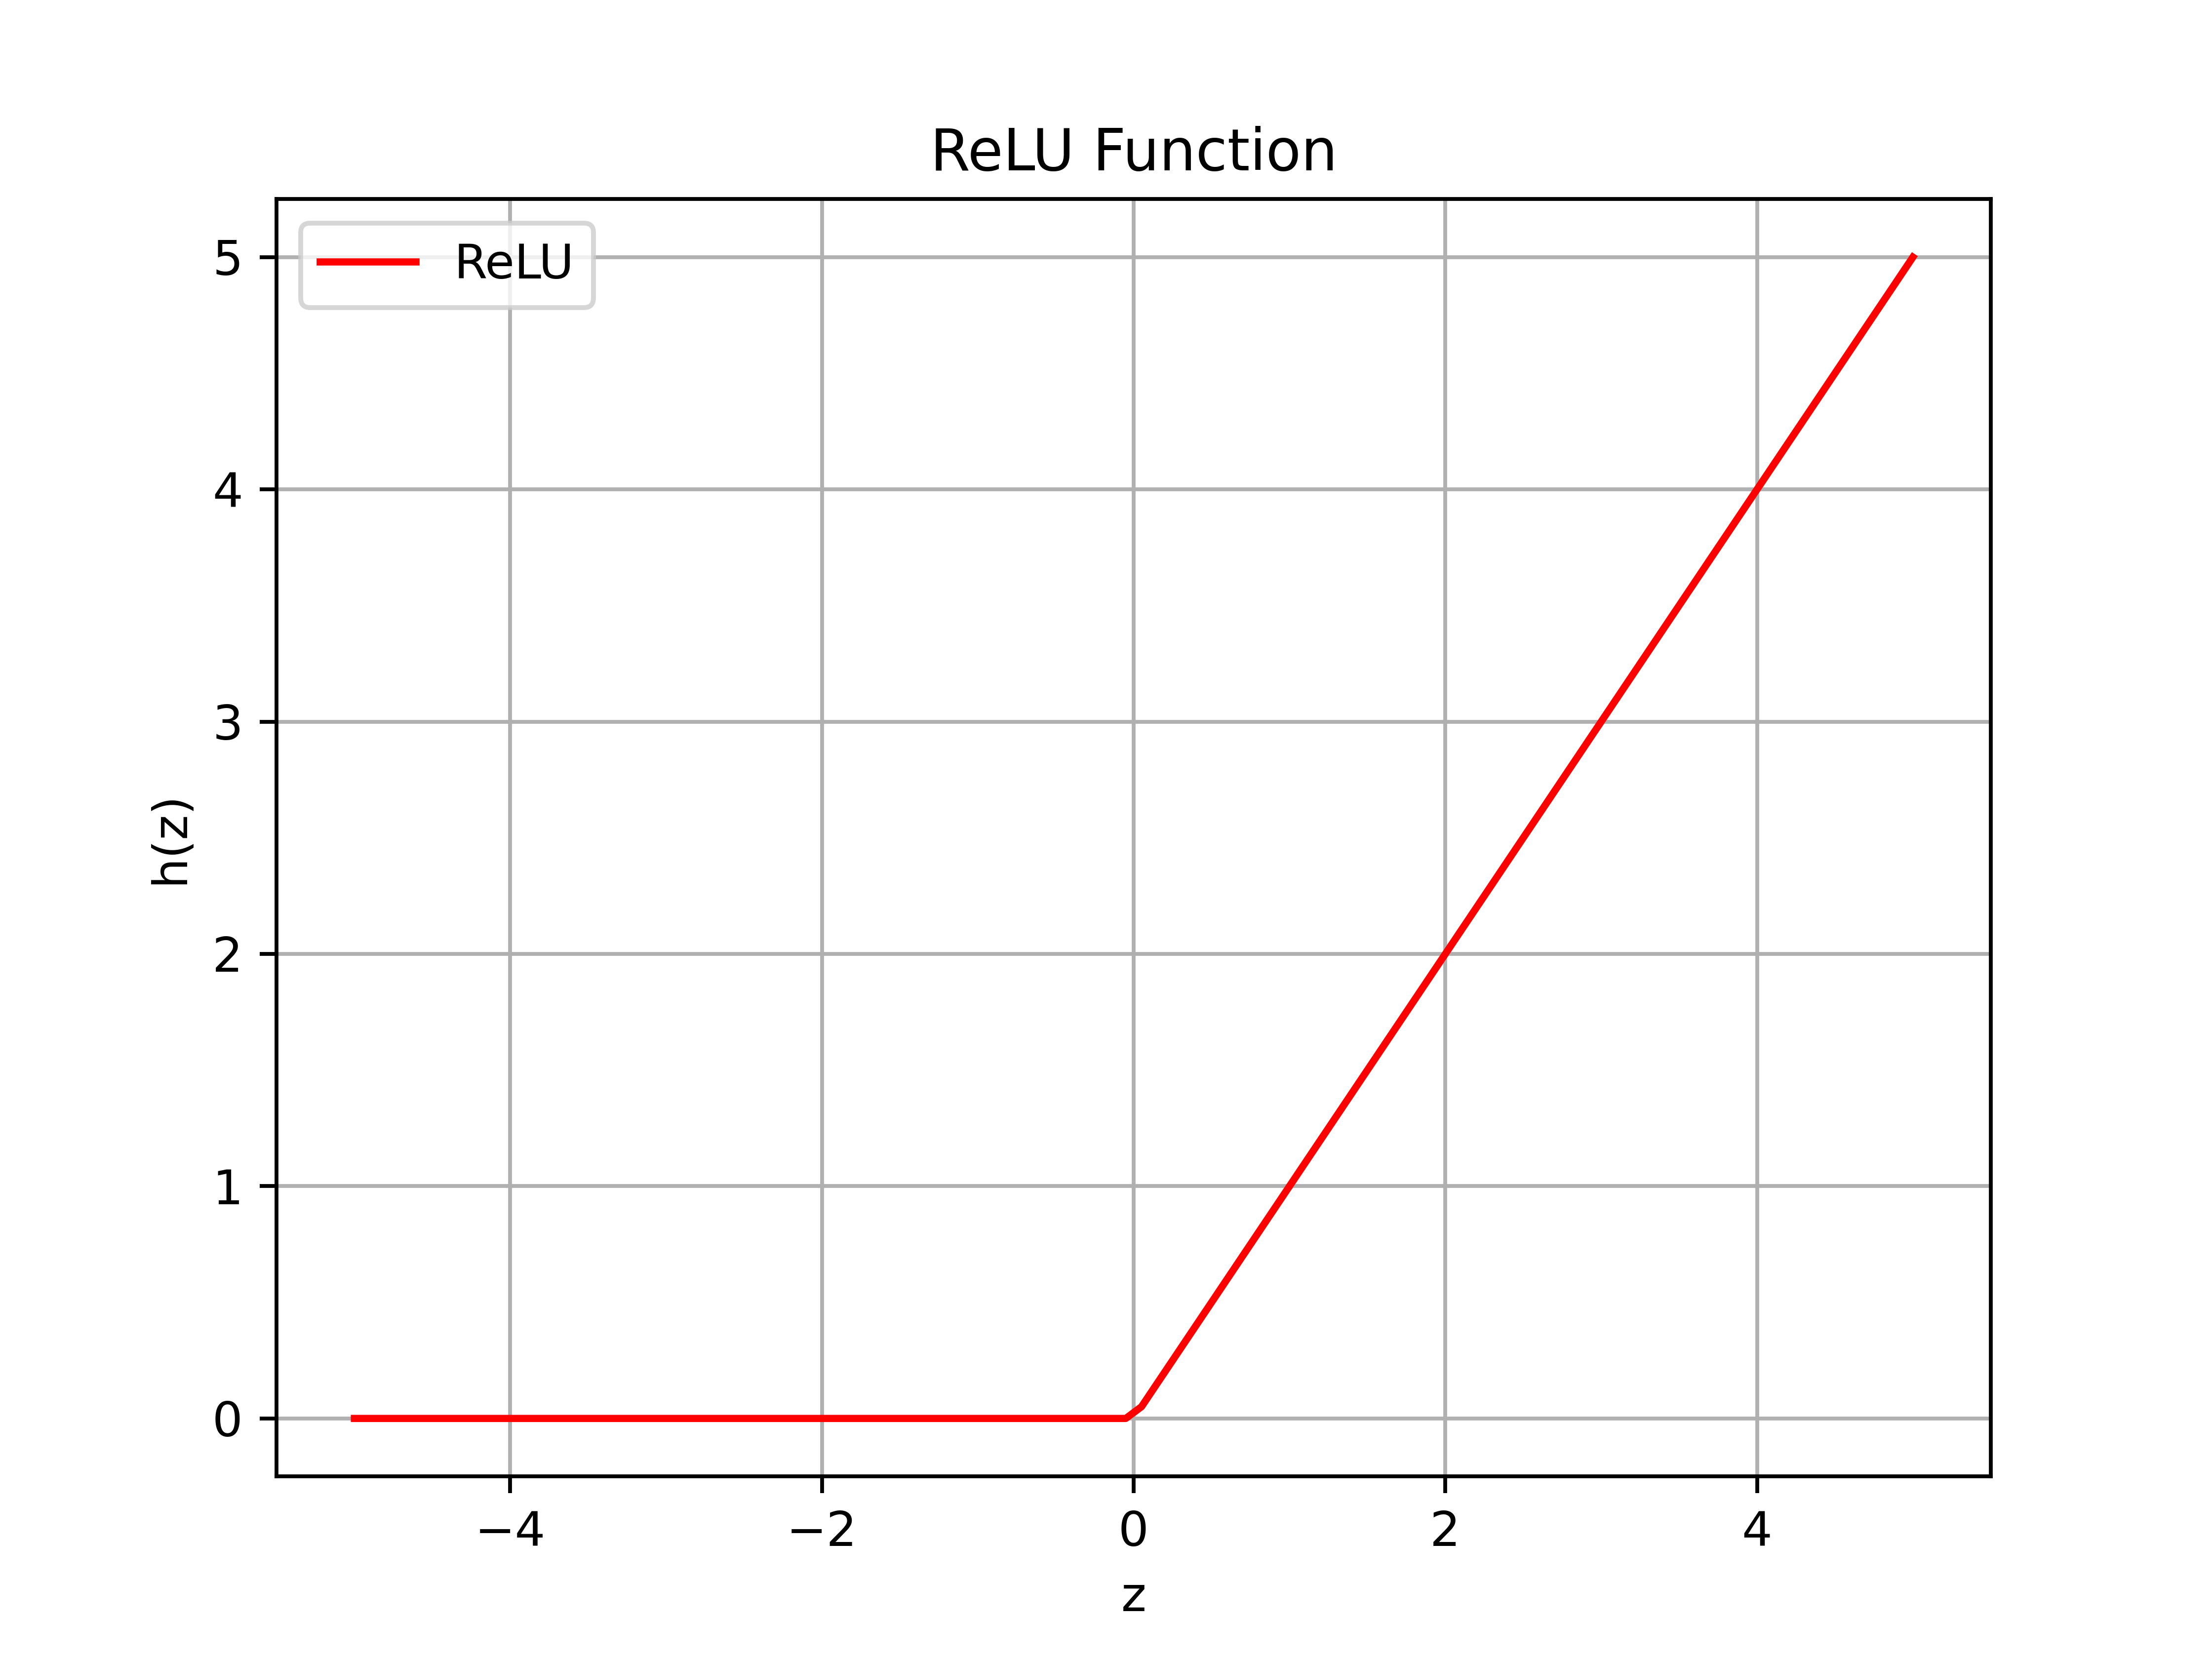
\includegraphics[width=0.65\textwidth]{imgs/relu_fun.png}
\caption{Illustration of ReLU Function. Image is generated using Python}\label{fig:relu}
\end{figure}

ReLU function ကို neural network ၏ hidden layer များအတွက် အဓိက အသုံးပြုသည်။ ဤ function (ညီမျှခြင်း- \ref{eqn:relu})သည် သုညထက်ကြီးသည့် input များအတွက် မူလတန်ဖိုးကို ပြန်ထုတ်ပေးသည်။ 

\subsection{Hyperbolic Tangent (tanh) Function} 

The hyperbolic tangent function, commonly denoted as $h_{tanh}(z)$ , is a mathematical function that maps input values to the range, $[-1,1]$ as shown in Figure \ref{fig:tanh}. It is similar to the sigmoid function but has a wider range and outputs negative values for negative inputs.  

\begin{equation}\label{eqn:tanh}
    h_{tanh}(z) = \frac{exp(z) - exp{-z}}{exp(z) + exp(-z)}
\end{equation} where $z$ is the pre-activation value. 

The tanh function is often used in hidden layers of neural networks as an activation function. It has been found to perform well in practice and is particularly useful when the data has zero mean, as it maps negative inputs to negative outputs and positive inputs to positive outputs, preserving the sign of the input.

\begin{figure}[h]%
\centering
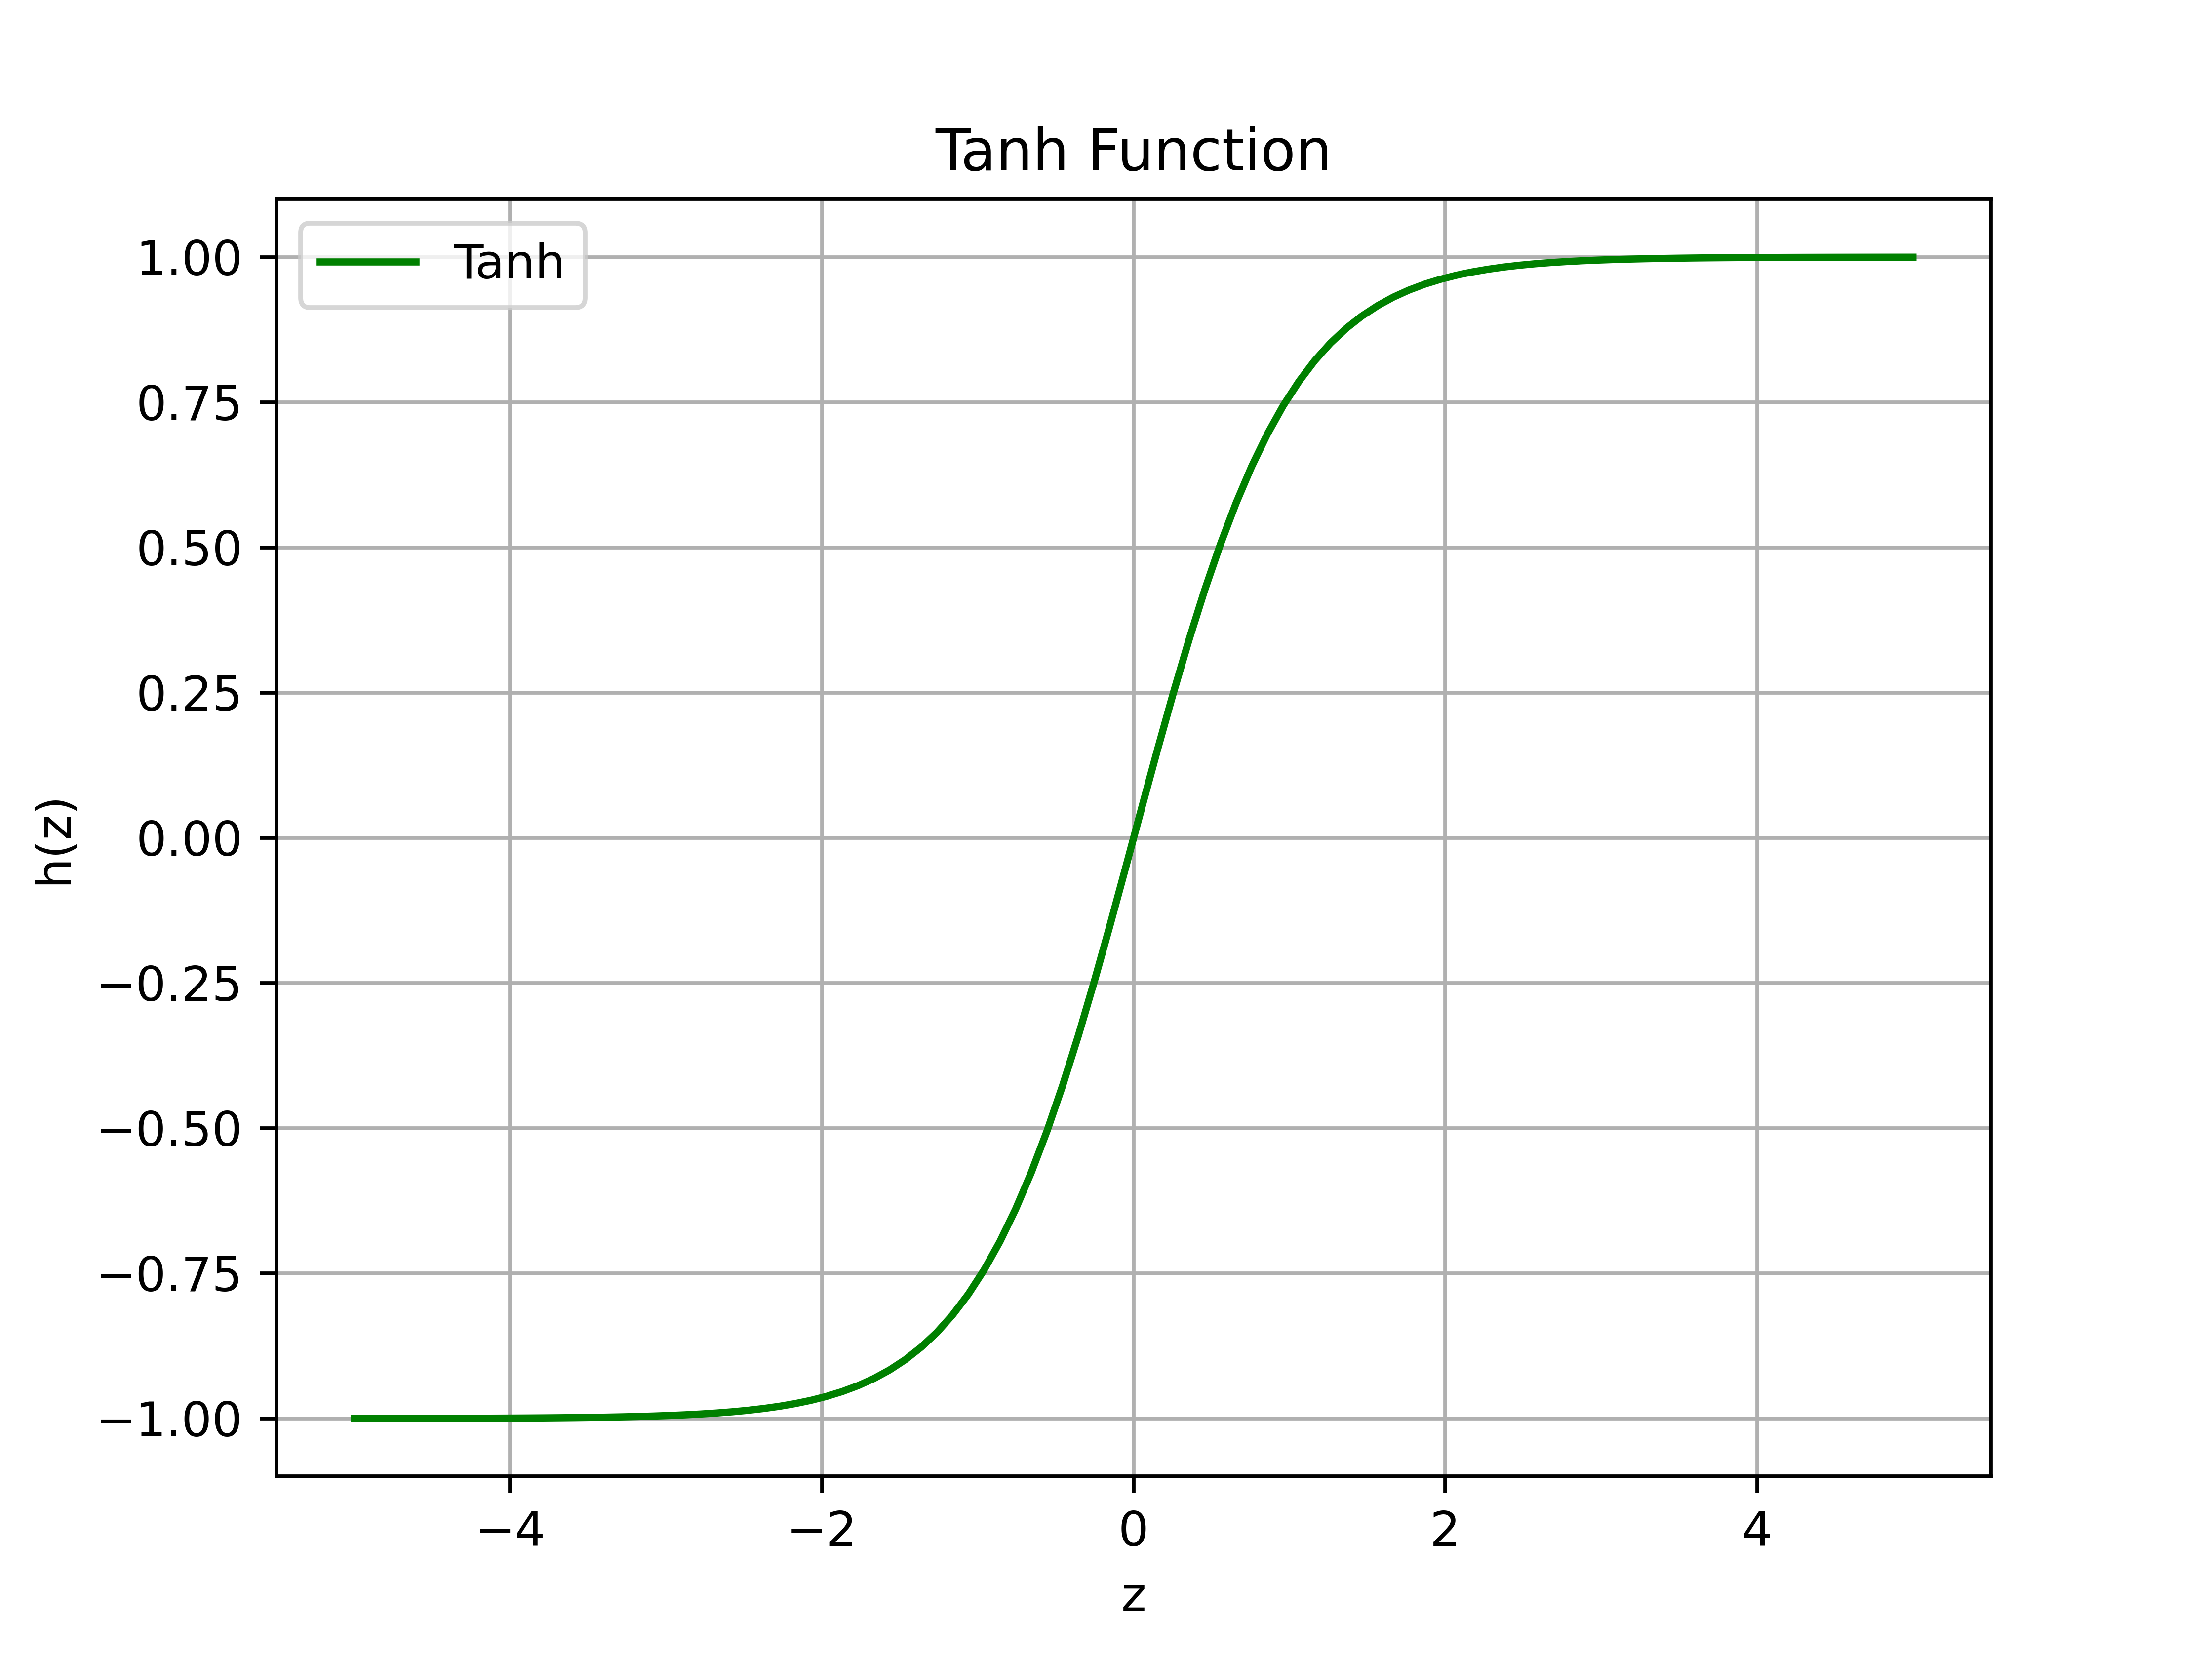
\includegraphics[width=0.65\textwidth]{imgs/tanh_fun.png}
\caption{Illustration of Hyperbolic Tangent (tanh) Function. Image is generated using Python.}\label{fig:tanh}
\end{figure}

Hyperbolic Tangent (tanh) Function သည် sigmoid Function နှင့် ဆင်တူသည်။ သို့သော် ပုံ (\ref{fig:tanh}) တွင်ပြသထားသည့် အတိုင်း $h_{tanh}(z)$ ၏ တန်ဖိုး သည် အနှုတ် တစ်နှင့် အပေါင်းတစ် အကြားတွင် ရှိသည်။ ထို့အပြင် အနှုတ်တန်ဖိုးရှိသည့် $z$ တန်ဖိုးများအတွက် အနှုတ် တန်ဖိုးကို ထုတ်ပေးပြီး သုညထက်ကြီးသည့် $z$ တန်ဖိုးများအတွက် အပေါင်းတန်ဖိုးကို ထုတ်ပေးရာ မူလ လက္ခဏာ တန်ဖိုးကို ထိန်းသိမ်းထားသည်ဟု ဆိုရမည်။ 
tanh function သည် လက်တွေ့ ပုစ္ဆာများတွက်ချက်ရာတွင် ရလဒ်ကောင်းများ ရရှိသည်ကို တွေ့ရပြီး hidden layer များအတွက် အဓိက အသုံးပြုသည်။

\newpage
\section{Forward Propagation}\label{sec:FProp}
Forward propagation is the process by which input data passes through the network layers, moving from left to right, to produce an output. It involves a series of mathematical operations that transform the input data, step by step, through each layer of the network. At the start of training, the neural network's weights and biases are typically unknown and initialized randomly.

\vspace{1.5em} 

\begin{figure}[h]%
\centering
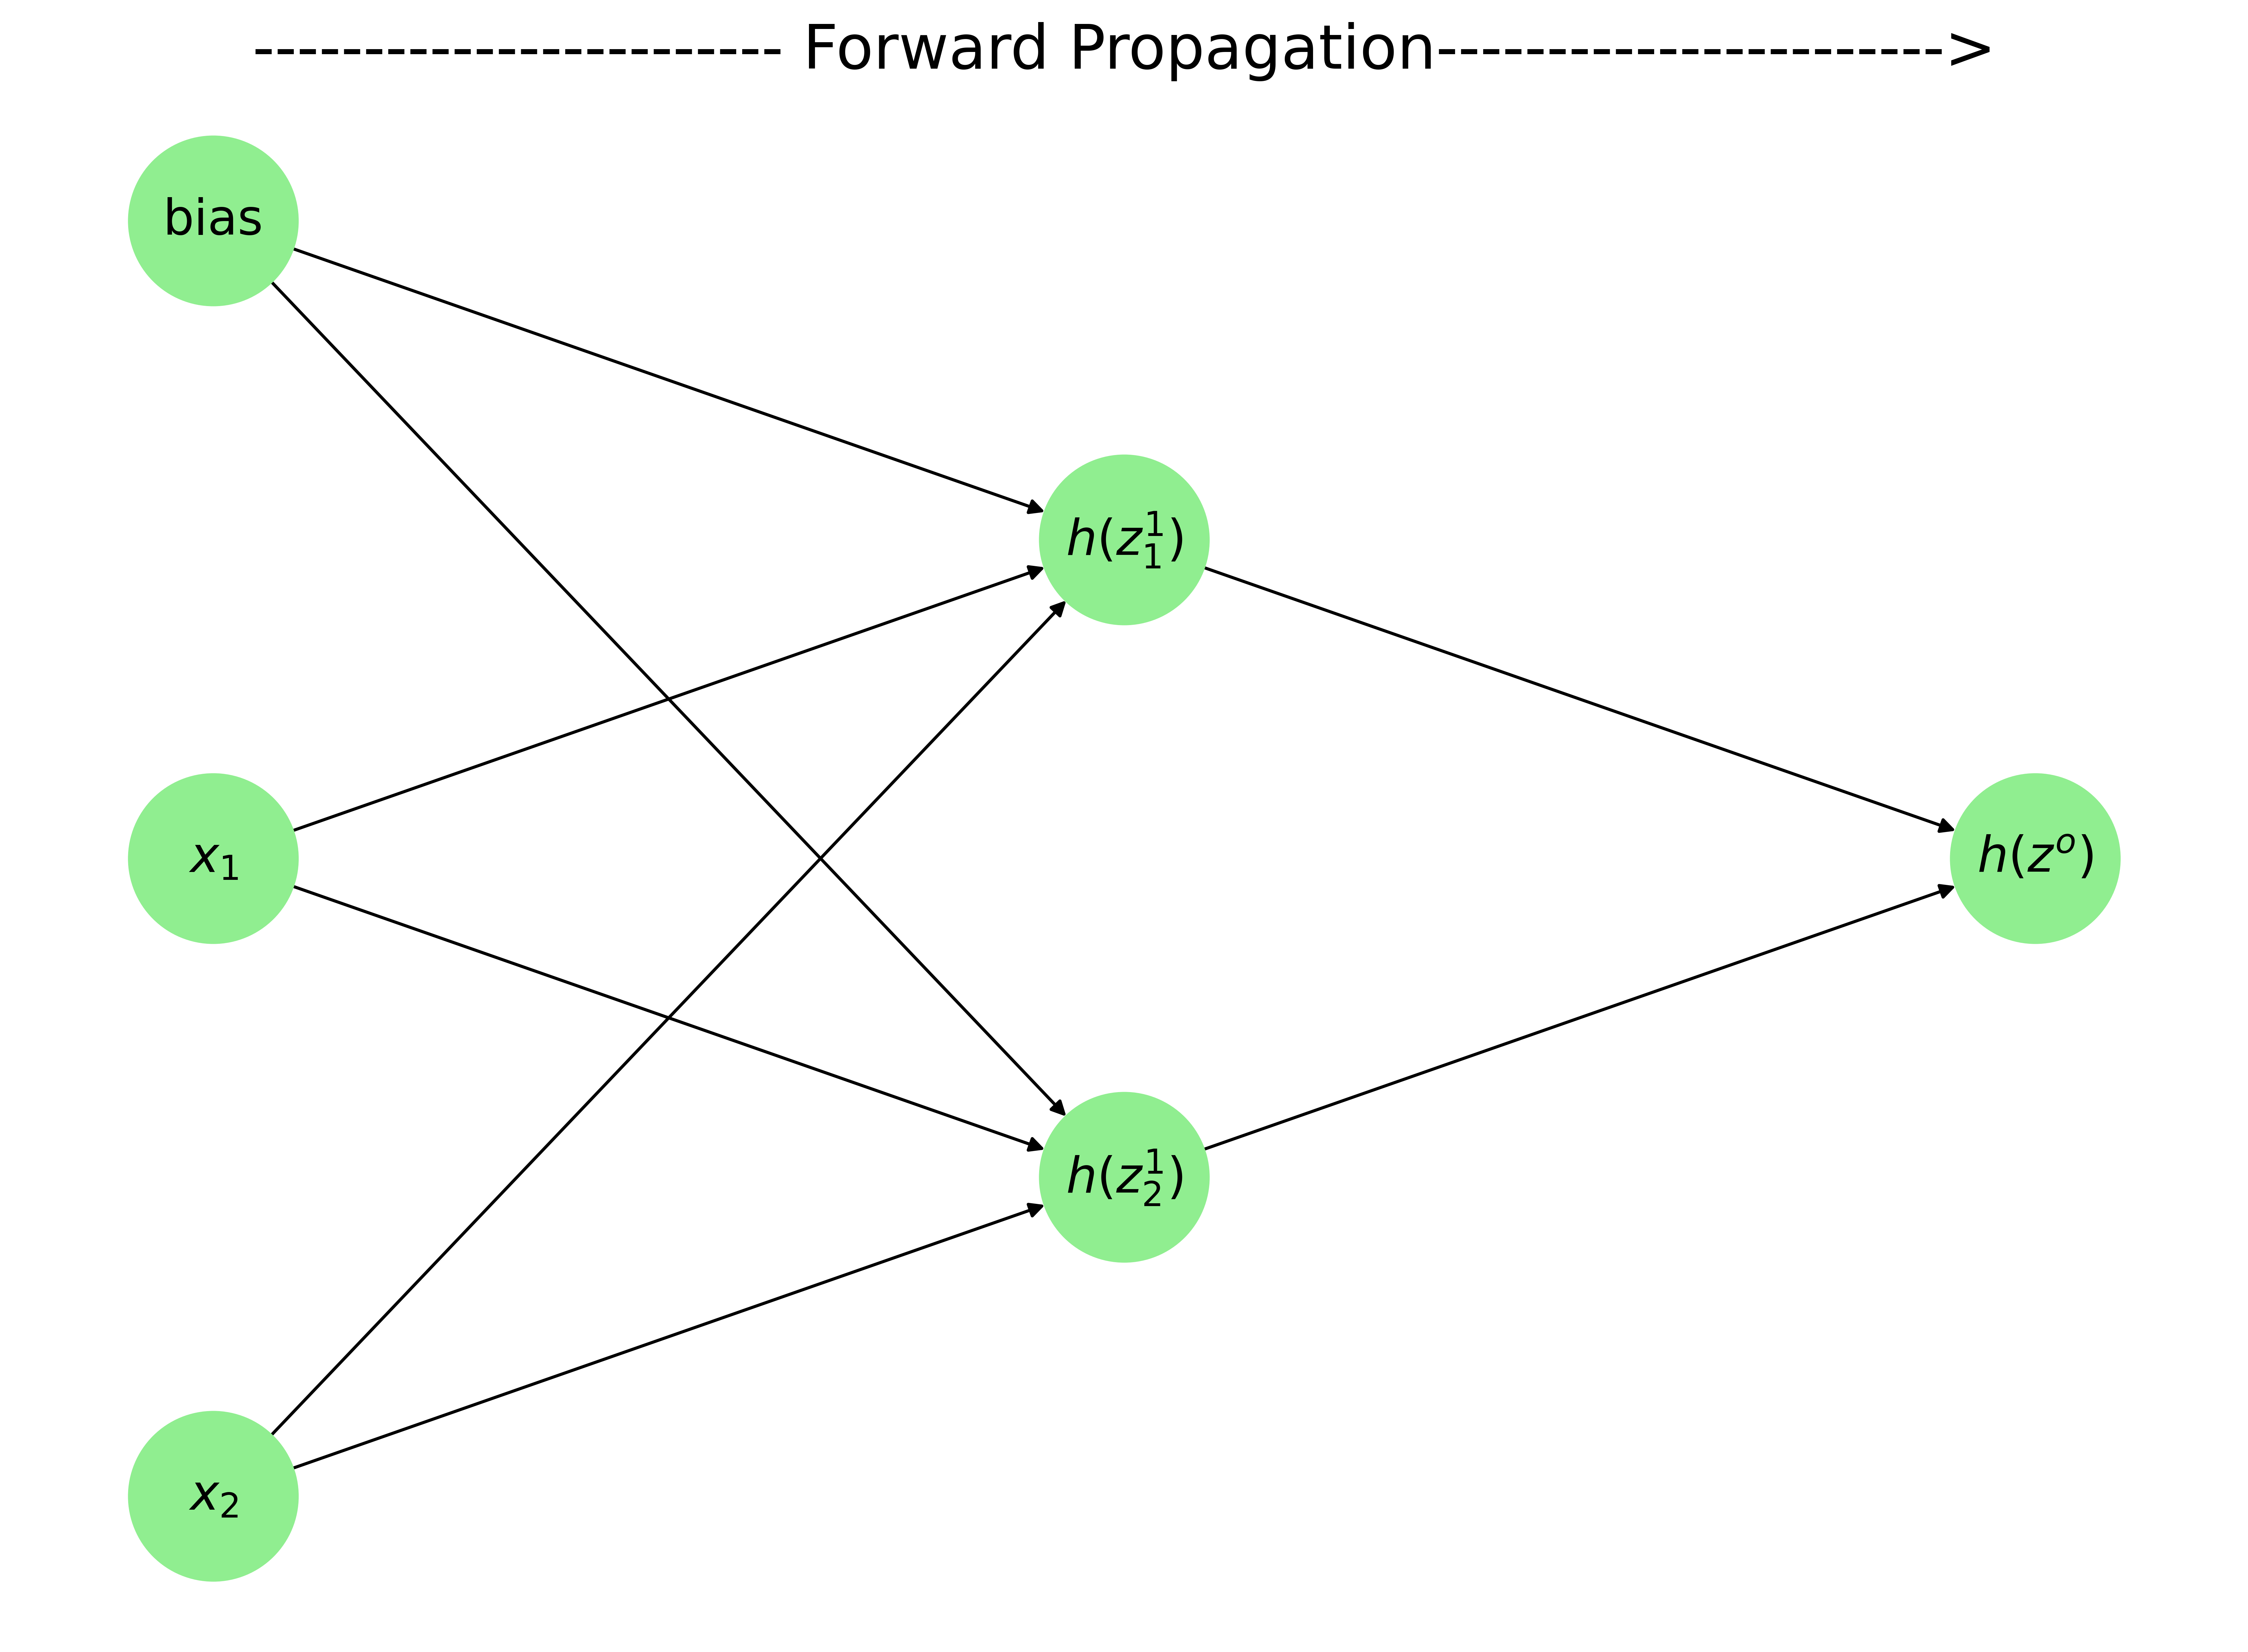
\includegraphics[width=0.75\textwidth]{imgs/fw_eg.png}
\caption{Multi-Layer Perception with one hidden layer and two input features. Image is generated using Python networkX Library}\label{fig:mlp_fwprop}
\end{figure}

\noindent Let's consider a simple example with a single hidden layer as shown in Figure \ref{fig:mlp_fwprop}:
\begin{itemize}
  \item \textbf{Input Layer}: Suppose we have two input features, $x_1$ and $x_2$.
  \item \textbf{Hidden Layer}: The hidden layer has two neurons. Each neuron receives $x_1$ and $x_2$ as inputs and computes the pre-activation values for each neuron, $z^1_1$ and $z^1_2$. 
  \begin{eqnarray}\label{enq:z12} 
    z^1_1  &=& \omega_{11} x_1 + \omega_{12}x_2 + b_1 \\
    z^1_2 &=& \omega_{21} x_1 + \omega_{22}x_2 + b_2
  \end{eqnarray} where $\omega_{i1}$ are the weights associated with the input features and the neurons in the hidden layer, and $b_i$ are the bias values.
  The outputs, $z^1_1$ and $z^1_2$ are then passed through an activation function and produces: 
  \begin{eqnarray}\label{enq:a12} 
    a_1 &=& h(z^1_1)\\
    a_2 &=& h(z^1_2)
  \end{eqnarray}  

  \item \textbf{Output Layer}: The output layer has one neuron, which takes $a_1$ and $a_2$ and computes the output:
    \begin{equation} \label{enq:Poutput} 
     y  = h (z^o) \text{ where } z^o = \omega_{o1} a_1 + \omega_{o2} a_2 + b_o
    \end{equation} $z^o$  is the pre-activation value at the output layer, $\omega_{oj}$ are the weights associated with the output and the neurons in the hidden layer, and $b_o$ is the bias value.
\end{itemize}

In forward propagation, the computed $y$ represents the predicted value using random weights. 

The objective of the machine learning model is to find the parameters (weights and bias) that produce the lowest errors between the actual and predicted values. This parameters are iteratively refined through backward propagation, where the model adjusts its parameters based on the calculated errors to improve its predictive accuracy. 

\noindent ပုံ \ref{fig:mlp} သည် hidden layer တစ်ခုပါ၀င်သော Multi-layer neural network ၏ ဥပမာဖြစ်သည်။  Input layer တွင် feature နှစ်ခု $x_1$ နှင့် $x_2$ တို့ရှိပြီး အဆိုပါ feature များသည် ကြားခံ layer ၏ Input များဖြစ်သည်။  ထို့နောက် $z^1_1$ နှင့် $z^1_2$ တန်ဖိုးကို ညီမျှခြင်း (\ref{enq:z12})ကို အသုံးပြု၍ တွက်ချက်သည်။ တနည်းဆိုသော် $z^1_1$ နှင့် $z^1_2$ ၏ တန်ဖိုးများသည် မြှောက်ဖော်ကိန်းများနှင့် မြှောက်ထားသည့် input feature များ၏ စုစုပေါင်းတန်ဖိုး ဖြစ်သည်။ 

ထို့နောက်  ကြားခံ layer ၏ output များဖြစ်သည့် $a_1$ နှင့် $a_2$ ၏ တန်ဖိုးကို activation function တစ်ခုကို သုံး၍ တွက်ချက်ရမည်။ အသုံးများသည့်  function များမှာ ReLU, Sigmoid, (သို့မဟုတ်) Tanh တို့ဖြစ်ကြသည်။ အဆိုပါ $a_1$ နှင့် $a_2$ သည် Output Layer အတွက် input များ ဖြစ်သည်။ ထို့နောက် final ရလဒ် ဖြစ်သော  $y$ ၏ တန်ဖိုးကို ညီမျှခြင်း \ref{enq:Poutput} ကို အသုံးပြု၍ တွက်ချက်သည်။ Classification ပုစ္ဆာများအတွက် Output Layer တွင် softmax  activation function ကို အသုံးပြုလေ့ ရှိပြီး regression ပုစ္ဆာများအတွက် linear function , $h(z^o) = z^o$ ကို အသုံးပြုကြသည်။ 

အထက်ပါ ညီမျှခြင်းများ (\ref{enq:z12}၊ \ref{enq:Poutput}) တွင် မြှောက်ဖော်ကိန်းများ ဖြစ်သော $\omega_{i}$ နှင့် $b_i$ ၏တန်ဖိုးများကို randomly သတ်မှတ်၍ တွက်ချက်ခြင်း ဖြစ်သည်။ Forward propagation မှ ရရှိသည့် $y$ ၏ တန်ဖိုးမှာ Multi-layer neural network Model မှ တွက်ချက်ပေးသည့် ခန့်မှန်းတန်ဖိုးသာ ဖြစ်သည်။ Machine learning model များ၏ ရည်ရွယ်ချက်မှာ ခန့်မှန်းတန်ဖိုး နှင့် training ဒေတာများ၏ မူလတန်ဖိုးကြား ခြားနားချက်ကို အနည်းဆုံးဖြစ်စေသည့် မြှောက်ဖော်ကိန်း များ $\omega_{i}$ နှင့် $b_i$ တန်ဖိုးများကို ရှာရန် ဖြစ်သည်။ 

\newpage
\section{Backward Propagation}\label{sec:bProp}

Backward propagation, also known as backpropagation, involves the iterative adjustment of the model's parameters (weights and biases) based on the calculated errors between the predicted and actual outputs. The Gradient descent is one of the fundamental algorithms used for updating the parameters. 
\begin{itemize}[f1]
  \item\textbf{Loss Computation}: After forward propagation, the model's prediction, $\hat{y}$ is compared to the actual target value $y$ using a loss function (e.g., mean squared error for regression, binary cross-entropy for binary classification, categorical cross-entropy for multi-class classification). This loss function computes the disparity between the predicted and actual outputs. 
  \item \textbf{Backpropagate Errors}: Once the loss is computed, the algorithm works backward through the network to calculate the gradient of the loss function with respect to each parameter. 
      \begin{itemize}
        \item \textbf{Output Layer}: Compute the gradients of weights and bias in the output layer using the chain rule
        \begin{eqnarray}\label{eqn:gradient1}
        % \nonumber to remove numbering (before each equation)
          \frac{\delta Loss}{\delta \omega_o} &=& \frac{\delta Loss}{\delta z^o } . \frac{\delta z^o}{\delta \omega_o}\\
         \frac{\delta Loss}{\delta b_o} &=& \frac{\delta Loss}{\delta z^o } . \frac{\delta z^o}{\delta b_o}
        \end{eqnarray}
        \item \textbf{Hidden Layer}: Compute the gradients of weights and bias in the hidden layer 
        \begin{eqnarray}\label{eqn:gradient2}
        % \nonumber to remove numbering (before each equation)
          \frac{\delta Loss}{\delta \omega_{hidden}} &=& \frac{\delta Loss}{\delta z^{hidden} } . \frac{\delta z^{hidden}}{\delta \omega_{hidden}}\\
         \frac{\delta Loss}{\delta b_{hidden}}           &=& \frac{\delta Loss}{\delta z^{hidden} } . \frac{\delta z^{hidden}}{\delta b_{hidden}}
        \end{eqnarray}
      \end{itemize}
  \item \textbf{Update Weights and Biases}: Adjust the weights and biases in both the output and hidden layers using the computed gradients and a learning rate. This step involves moving in the opposite direction of the gradients to minimize the loss function. 
      \begin{eqnarray}\label{eqn:update}
        % \nonumber to remove numbering (before each equation)
          \omega_o^{new} &=& \omega_o^{old} - \text{learning rate} \times \frac{\delta Loss}{\delta \omega_o}\\
          b_o^{new}          &=& b_o^{old} - \text{learning rate} \times \frac{\delta Loss}{\delta b_o}\\
          \omega_{hidden}^{new} &=& \omega_{hidden}^{old} - \text{learning rate} \times \frac{\delta Loss}{\delta \omega_{hidden}}\\
          b_{hidden}^{new}          &=& b_{hidden}^{old} - \text{learning rate} \times \frac{\delta Loss}{\delta b_{hidden}}   
        \end{eqnarray}
\end{itemize}

Both forward and backward propagation are repeated for multiple \textbf{epochs} until the model converges or until a stopping criterion is met.

\begin{definition}\label{def:epoch}
An \textbf{epoch} refers to one complete pass through the entire training dataset. During each epoch, the neural network performs forward and backward propagation (calculating predictions, computing loss, and updating weights) for every sample in the training dataset.
\end{definition}

\newpage
\noindent Neural Network Model တစ်ခုကို Training ပြုလုပ်ရာတွင် forward နှင့် backward propagation ကို ကြိမ်ဖန်များစွာ ပြုလုပ်ပြီး ခန့်မှန်းတန်ဖိုးနှင့် မူလတန်ဖိုး၏ ခြားနားချက် အနည်းဆုံးဖြစ်စေမည့် $\omega_{i}$ နှင့် $b_i$ ၏ တန်ဖိုးများကို ရှာဖွေရသည်။ Forward propagation အဆင့်တွင် $\hat{y}$ ၏ တန်ဖိုးကို တွက်ချက်နိုင်ရန်အတွက်  neural network ၏ input layer မှ output layer တဆင့်ချင်း (ဘယ်မှညာသို့) တွက်ချက်ရသည်။ 

Backward propagation အဆင့်တွင်မူ output layer မှ  input layer သို့ (ညာမှ ဘယ်သို့) ပြန်သွားပြီး layer တစ်ခုချင်းစီတွင် ရှိသည့် Parameter များ၏ gradients တန်ဖိုးများကို ညီမျှခြင်း \ref{eqn:gradient1} နှင့် \ref{eqn:gradient2} တို့ကို အသုံးပြု၍ တွက်ချက်သည်။ ထို့နောက် $\omega_{i}$ နှင့် $b_i$ များ၏ တန်ဖိုးကို ညီမျှခြင်း \ref{eqn:update} ကို အသုံးပြု၍ update ပြုလုပ်ပေးရသည်။ 

Forward နှင့် backward propagation process - ၂ ခု လုံးပါ၀င်သော Cycle တစ်ခုကို epoch ဟုခေါ်ဆိုပြီး Neural Network Model များ တည်ဆောက်ရာတွင် Programmer/developer မှ epoch အရေအတွက်ကို သတ်မှတ်ပေးရန် လိုအပ်သည်။ 

\newpage
\section{Practical Implementation}\label{sec:hands-on}
In this section, two practical projects are presented to reinforce the concepts learned in the previous sections. These projects are designed to provide hands-on experience and deepen your understanding through real-world applications. By working through these projects, you will be able to apply the theoretical knowledge in practical scenarios, thereby solidifying your learning and enhancing your skills. 

Walk-through videos are provided via the author's YouTube channel \cite{web:myoYouTube}. You can watch the videos while reading and implementing the codes along.

ဤအခန်းတွင် လက်တွေ့  industry တွင် အသုံး၀င်သည့် project နှစ်ခုကို Neural Network အသုံးပြု၍ တည်ဆောက်ပုံ တည်ဆောက်နည်း အဆင့်ဆင့်ကို ဖော်ပြသွားမည် ဖြစ်သည်။ Deep Learning ကို လေ့လာရာတွင် project များကို လက်တွေ့  လိုက်ပါ လေ့ကျင့်ရန် လိုအပ်ပါသည်။ ဤ လေ့ကျင့်ခန်းများကို လေ့လာရာတွင် အထောက် အကူဖြစ်စေရန်အတွက် project ကို ရှင်းပြသည့် video များကို YouTube Channel တွင် တင်ပေးထားပြီး ဖြစ်သည်။ သက်ဆိုင်ရာ Project အလိုက် ပေးထားသည့် လင့်တွင် သွားရောက် ကြည့်ရှု့နိုင်သည်။ 

\subsection{Regression: Resale House Price Prediction}\label{sec:SGHDB}

House price prediction is a significant application of machine learning with substantial implications for various stakeholders in the real estate market. The deployment of these models into commercial platforms enhances decision-making processes, market analysis, and strategic planning. Leveraging large datasets and advanced algorithms, machine learning (ML) models have significantly transformed the landscape of house price prediction, yielding remarkably accurate predictions.

In today's digital landscape, numerous real estate websites and applications integrate ML models to provide price estimates for listed properties. This integration not only elevates user experience and engagement but also empowers buyers and sellers to make informed decisions. Additionally, it enables real estate agents to offer enhanced services and assists investors in identifying opportunities within the market. Continuously improving ML models for higher accuracy is a collaborative effort between academia and industry. Real estate data is dynamic, with various factors influencing prices differently across regions. Therefore, it is essential to develop models tailored to each market's unique characteristics.

In Singapore, an HDB (Housing and Development Board) estate typically refers to a large residential area comprising multiple HDB blocks. Each block is a high-rise building containing numerous housing units, commonly known as HDB flats or apartments.  All HDB properties in Singapore typically have a 99-year lease term.

First-time buyers acquire their properties directly from the Singapore government, while resale transactions involve the buying and selling of units among Singapore residents. Each transaction is recorded by the Singapore Housing and Development Board to track ownership. In earlier records, the approval date by HDB is considered the transaction date, but after 2014, the registration date is recorded. These two dates are typically within a month of each other, resulting in minimal fluctuation. However, the resale prices recorded by HDB should be considered indicative only, as the actual resale prices agreed upon between buyers and sellers depend on many factors. Being able to estimate the resale price based on the properties of a flat, such as location, area, and other factors, helps both buyers and sellers make informed decisions.

This section explains, step by step, how to develop a Neural Network (deep learning) model for predicting resale prices of public housing flats (HDB flats) in Singapore. 

\begin{remark}
This work is inspired by a project assignment given to my students during the Supervised Machine Class (iSTAR) of 2024. In this course, students were tasked with developing a regression model to predict housing prices for houses or flats in the region. While the codes and explanations are my original work, the project context was developed as part of the coursework to provide practical learning experiences.
\end{remark}

Real estate Online Platform များတွင်  Machine learning model များကို ထည့်သွင်း အသုံးပြုလာနိုင်ခြင်းသည် အိမ်ခြံမြေစျေးကွက်ကို စိတ်၀င်စားသူများအတွက် အရေးပါသော အရွေ့ တစ်ခု ဖြစ်သည်။ ဒေတာ အချက်အလက်များ တနေ့တခြား များပြားလာခြင်း နှင့် အတူ အချက်အလက်မှန်ကန်သည့် ဒေတာများကို အစိုးရ website များ အပါအ၀င် အဖွဲ့အစည်းအမျိုးမျိုးက အများပြည်သူ အသုံးပြုနိုင်အောင်ဖွင့်ပေးလာကြသည်။ ထိုသို့ ဒေတာများ အလွယ်တကူ ရရှိနိုင်ခြင်း၊ ကွန်ပြူတာများ အဆင့်မြင့်လာခြင်းတို့သည် အိမ်ခြံမြေ နှင့် တိုက်ခန်းများ၏ စျေးနှုန်းခန့်မှန်းရန်အတွက် ပိုမိုကောင်းမွန်သည့် Machine learning model များ တည်ဆောက်ရန် အထောက်အပံ့ကောင်းများ ဖြစ်သည်။ 

အိမ်ခြံမြေစျေးကွက်၏ သဘော သဘာ၀မှာ နေရာဒေသတစ်ခုနှင့် တစ်ခု အပေါ်မူတည်၍ အချက်အလက်များ ကွဲပြားကြသည်။ သို့ဖြစ်ရာ Machine learning model တစ်ခုထဲကို နေရာအမျိုးမျိုးတွင် အသုံးပြုရန်မှာ မဖြစ်နိုင်ပေ။ နိုင်ငံ (သို့ မဟုတ်) မြို့နယ် အလိုက် ရရှိနိုင်သော ဒေတာအချက်အလက်များကို အသုံးပြု၍ တည်ဆောက်မှသာလျှင် ပို၍ တိကျသော စျေးနှုန်းခန့်မှန်းချက်များကို ရရှိနိုင်မည် ဖြစ်သည်။ 

Singapore နိုင်ငံတွင် အများပြည်သူများ သက်သက်သာသာနှင့် ၀ယ်ယူနေထိုင်နိုင်ရန် အစိုးရအဖွဲ့အစည်းတစ်ခုဖြစ်သည့် HDB (Housing and Development Board) မှ တာ၀န်ယူ ဆောက်လုပ်သည့် တိုက်ခန်းများကို HDB တိုက်ခန်းများဟု ခေါ်ဆိုကြသည်။ မြို့နယ်အလိုက်  HDB အိမ်ယာများစွာ ရှိပြီး အိမ်ယာတစ်ခုတွင် အထပ်မြင့် အဆောက်အအုံတစ်ခုမက ပါ၀င်သည်။ အဆိုပါ အဆောက်အအုံများကို Singapore အစိုးရမှ ပိုင်ဆိုင်ပြီး ပြည်သူကို ရောင်းချသည့် သက်တမ်းမှာ ၉၉ နှစ်သာ ဖြစ်သည်။ တိုက်သက်တမ်းလွန်သည့် တိုက်ခန်းများကို အစိုးရက ဖြိုဖျက်ပြီး အသစ်ပြန်လည်ဆောက်လုပ်လေ့ရှိသည်။ အသစ်ဆောက်လုပ်ပြီးစီးသည့် HDB တိုက်ခန်းများကို Singapore အစိုးရထံမှသာ တိုက်ရိုက် ၀ယ်ဆိုနိုင်သည်။ သတ်မှတ် ကာလတစ်ခု  (များသောအားဖြင့် ၅ နှစ်) ကျော်လွန်သွားပါက HDB တိုက်ခန်းဟောင်းများကို နေထိုင်သူ အချင်းချင်းကြား ပြန်လည်ရောင်းချခြင်း၊ ၀ယ်ယူခြင်းများ ပြုလုပ်နိုင်သည်။ 

သို့သော် အရောင်းအ၀ယ် ပြုလုပ်မည်ဆိုပါက Singapore အစိုးရ (HDB) ထံမှ တရား၀င် ခွင့်ပြုချက်ရယူရန်လိုအပ်သည်။ အဆိုပါ အရောင်းအ၀ယ်မှတ်တမ်းတိုင်းကို HDB တွင် စနစ်တကျ စာရင်းသွင်းထားရှိသည်။ အစောပိုင်း စာရင်းသွင်းချက်များတွင် HDB မှ ခွင့်ပြုပေးလိုက်သည့် နေ့ကို အရောင်းအ၀ယ်ပြုလုပ်သည့်နေ့ဟု သတ်မှတ်ခဲ့ကြသော်လည်း နောက်ပိုင်း မှတ်တမ်းများတွင်မူ HDB တွင် မှတ်တမ်းတင်သည့်နေ့ကို အရောင်းအ၀ယ်ပြုလုပ်သည့်နေ့ဟု သတ်မှတ်သည်။ ယေဘူယျအားဖြင့်  HDB မှ ခွင့်ပြုပေးလိုက်သည့် နေ့နှင့် မှတ်တမ်းတင်သည့်နေ့မှာ တစ်လအတွင်းဖြစ်သဖြင့် ကြားထဲတွင် စျေးနှုန်း အပြောင်းအလဲ ဖြစ်လေ့မရှိပါ။ သို့သော် ရောင်းသူနှင့် ၀ယ်သူ အကြားသဘောတူညီချက်များကို မူတည်၍ HDB ၏ မှတ်တမ်းရှိ စျေးနှုန်းများနှင့် ပြင်ပပေါက်စျေးများသည် အနည်းငယ် ကွာဟနိုင်သည်။ 

ဤသင်ခန်းစာတွင် Singapore နိုင်ငံရှိ HDB တိုက်ခန်းများ၏ စျေးနှုန်းကို ခန့်မှန်းသည့် Neural Network Model တစ်ခုအား Keras Library ကို အသုံးပြု၍ တည်ဆောက်သည့် အဆင့်ဆင့်ကို ရှင်းပြသွားမည်။ 

\subsubsection{Dataset}

The dataset used for this project is obtained from the Singapore government's open data portal \cite{web:SGdata}, which provides various datasets relevant to different aspects of public administration, urban planning, health, transportation, and other sectors managed by the government. Using a reliable data source is crucial for building an accurate and robust machine learning model.

The dataset includes detailed information on resale transactions of HDB flats between January 1, 2017, and March 30, 2024. The dataset contains 175,672 rows and 11 columns and was downloaded on May 23, 2024.  Further details regarding the dataset are outlined in Table \ref{tab:data_attributes}. 

\vspace{0.5em}

\begin{table}[h]
\centering
\caption{Data Attributes of Singapore HDB Flat (January - 2017 to March  - 2024}
\label{tab:data_attributes}
{\scriptsize
\begin{tabular}{|c|l|l|l|l|}
\hline
\textbf{Num} & \textbf{Data Attributes} & \textbf{Column Name} & \textbf{Data Type} & \textbf{Description} \\ \hline
1 & Month & month & Text (Date-Time) & Month and Year of sale \\ \hline
2 & Town & town & Text & Designated residential area \\ \hline
3 & Flat type & flat\_type & Text & Classification of units by room size \\ \hline
4 & Block & block & Text & The Block number where the unit sold located \\ \hline
5 & Street name & street\_name & Text & Street name of the unit sold located \\ \hline
6 & Storey range & storey\_range & Text & Estimated range of floors the unit sold was located on \\ \hline
7 & Floor area sqm & floor\_area\_sqm & Numeric & Total interior space within the unit, measured in square meters \\ \hline
8 & Flat model & flat\_model & Text & Classification of units by generation \\ \hline
9 & Lease commence date & lease\_commence\_date & Numeric & Starting point of a lease agreement (Year) \\ \hline
10 & Remaining lease & remaining\_lease & Text & Remaining amount of time left on the lease (Years and Months) \\ \hline
11 & Resale price & resale\_price & Numeric & Resale Price of the flat sold \\ \hline
\end{tabular}}
\end{table}

\noindent ယခု Project တွင် အသုံးပြုသည့် ဒေတာကို Singapore အစိုးရ၏ open data portal \cite{web:SGdata} မှ ရယူထားခြင်းဖြစ်သည်။ အဆိုပါ website ကို Singapore အစိုးရ အဖွဲ့အစည်းတစ်ခုဖြစ်သည့် GovTech မှ တည်ထောင်ထားခြင်းဖြစ်ပြီး Singapore ၀န်ကြီးဌာန အချို့ နှင့် အစိုးရ အဖွဲ့အစည်းများ၏ ဒေတာများကို ပြည်သူအများ အသုံးပြုနိုင်ရန် တင်ပေးထားသည်။ AI နှင့်  Machine Learning Project များ ပြုလုပ်ရာတွင် ယုံကြည် စိတ်ချရသည့် ဒေတာ အချက်အလက်များကို ရယူနိုင်ရန် အရေးကြီးသည်။ 

ဤ dataset ကို ၂၀၂၄ ခုနှစ် မတ်လ ၂၃ ရက်နေ့တွင် အထက်ပါ website မှ download ရယူခဲ့ပြီး ၄င်း dataset တွင် ၂၀၁၇ ဇန်န၀ါရီလ ၁ ရက်မှ ၂၀၂၄ မတ်လ ၃၁ ရက်နေ့အထိ ရောင်းချထားသော Singapore HDB တိုက်ခန်းများ၏ အရောင်းစာရင်းများ ပါ၀င်သည်။ စုစုပေါင်းပါ၀င်သည့် အရောင်း တိုက်ခန်း အရေအတွက်မှာ တစ်သိန်း ခုနစ်သောင်း ငါးထောင် ခြောက်ရာ ခုနစ်ဆယ့် နှစ်ခု (၁၇၅,၆၇၂)  ဖြစ်ပြီး ရောင်းချမှုအတွက် စာရင်းသွင်းသည့် ခုနှစ်နှင့်လ၊ တိုက်ခန်း အကျယ်အ၀န်း၊ အမျိုးအစား၊ တည်နေရာ စသည်ဖြင့် Column -၁၁ ခု ပါ၀င်သည်။ အထက်ပါ ဇယားတွင် ဖော်ပြထားသည့် dataset တွင် ပါ၀င်သော အချက်အလက်များ၏ အဓိပ္ပာယ် ဖွင့်ဆိုချက်အသေးစိပ်မှာ အောက်ပါအတိုင်း ဖြစ်သည်။ 

\begin{itemize}
  \item month--> တိုက်ခန်း ရောင်းချမှုကို စာရင်းသွင်းသည့် ခုနှစ်၊ လ။
  \item town-->  တိုက်ခန်း  တည်ရှိသည့် မြို့အမည်။ 
  \item Flat type --> တိုက်ခန်း အမျိုးအစား -- ပါ၀င်သည့် အခန်းအရေအတွက်ကို မူတည်၍ သတ်မှတ်ပြီး အမျိုးအစား ၇ ခု ရှိသည်။ 
  \item Block-->တိုက်ခန်း တည်ရှိသည့် အဆောက်အအုံ၏ နံပါတ်။
  \item Street name--> တိုက်ခန်း  တည်ရှိသည့် လမ်းအမည်။ 
  \item Storey range--> တိုက်ခန်း တည်ရှိသည့် အလွှာ/အထပ် အုပ်စု ။ 
  \item Floor area sqm--> တိုက်ခန်း၏ ဧရိယာ အကျယ်အ၀န်း ( square meter နှင့် ပေးထားသည်။)
  \item Flat model--> တိုက်ခန်း၏ မော်ဒယ် (တည်ဆောက်သည့် ပုံစံကို မူတည်၍ သတ်မှတ်ပြီး အမျိုးအစား ၂၁ မျိုး ရှိသည်)။ 
  \item Lease commence date--> Housing and Development Board မှ စတင်ရောင်းချသည့် ရက်စွဲ။ 
  \item Remaining lease--> တိုက်ခန်း၏ လက်ကျန် သက်တမ်း (အစိုးရ ခွင့်ပြုသည့် သက်တမ်းမှာ ၉၉ နှစ်ဖြစ်သည်။)
  \item Resale price--> စာရင်းသွင်းသည့် ရောင်းချ စျေးနှုန်း။ 
\end{itemize}
\begin{remark}
တိုက်ခန်း ရောင်းချမှုကို HDB တွင် စာရင်းသွင်းသည့် ရက်နှင့် အမှန်ရောင်းချမှုသည် များသောအားဖြင့် တစ်လအတွင်း ဖြစ်သည်။
\end{remark}
\subsubsection{Data Preprocessing}
The dataset is well maintained and prepared by the Singapore government's open data portal \cite{web:SGdata}. There is no missing data, which simplifies the preprocessing steps. 

\noindent ဤ dataset သည် Singapore အစိုးရ၏ မှ data portal ရယူထားသည်ဖြစ်ရာ ဒေတာများမှာ အမှားအယွင်းကင်းပြီး အချက်အလက်ပြည့်စုံသည်။ သို့သော် အချို့ အချက်အလက်များကိုမူ Neural Network (deep learning model) တစ်ခု တည်ဆောက်ရန်အတွက် အဆင်သင့် ဖြစ်စေရန် ပြင်ဆင်မှု အချို့ ပြုလုပ်ရသည်။ 

\subsubsection{Data Preprocessing: Data Cleaning}
\begin{enumerate}
    \item In the given dataset, \textit{\textbf{Lease commencement date}} and \textit{\textbf{remaining lease}} are two attributes conveying almost identical information. The former signifies the year when the lease for the property commenced. The latter denotes the number of years remaining on the lease at the time of the transaction. Since all HDB properties in Singapore typically have a 99-year lease term, these two attributes are related by:
        \begin{equation}\label{eqn:lease_relation}
           \text{remaining lease} = 99 - (\text{sold year} - \text{lease commencement year})
        \end{equation} As a result, the \textit{\textbf{Lease commencement date}} attribute is dropped to avoid redundancy.
        
    \item Similarly, three features relate to the location of the flat: '\textbf{\textit{block number}}', '\textit{\textbf{street name}}', and '\textit{\textbf{town}}'. While '\textbf{\textit{block number}}', and '\textit{\textbf{street name}}' provide the exact location of the resale flat, these three features are highly correlated. Hence, only the '\textit{\textbf{town}}'. attribute is considered, and the other two attributes are dropped.
\end{enumerate}

ဤ dataset တွင် တိုက်ခန်း၏ သက်တမ်းနှင့် ပတ်သတ်၍ အချက် ၂ ခု ပေးထားသည်ကို တွေ့ရသည်။ ပထမ အချက် ဖြစ်သော  \textit{\textbf{Lease commencement date}} သည် တိုက်ခန်းကို အစိုးရမှ စတင်ရောင်းချသည့် ရက်စွဲဖြစ်ပြီး အခြား အချက်မှာမူ တိုက်ခန်း၏ လက်ကျန် သတ်တမ်း \textit{\textbf{remaining lease}} ဖြစ်သည်။  အစိုးရ သတ်မှတ်ထားသည့် တိုက်ခန်း၏ သက်တမ်းမှာ ၉၉ ခုနှစ် ဖြစ်ရာ အဆိုပါ တိုက်ခန်းကို လက်လွှဲရောင်းချချိန်တွင် ရှိမည့် တိုက်ခန်း၏ လက်ကျန်သက်တမ်းသည် ၉၉ နှစ် ထဲမှ လက်ရှိသက်တမ်းကို နှုတ်ခြင်းဖြစ်သည်။   ဥပမာ -- ၁၉၉၄ တွင် အစိုးရမှ စတင်ရောင်းချသော တိုက်ခန်းများ၏ သက်တမ်းသည် ၂၀၂၄ ခုနှစ်တွင် သက်တမ်း နှစ် (၃၀) ရှိနေပြီ ဖြစ်သည်။ သို့ဖြစ်ရာ အဆိုပါ တိုက်ခန်းကို ယခု အချိန် (၂၀၂၄ ခုနှစ်) တွင် ရောင်းချမည်ဆိုပါက တိုက်ခန်း၏ လက်ကျန်သက်တမ်းမှာ ၆၉ နှစ် (၉၉-၃၀)  ဖြစ်သည်။ 

ဤ Project အတွက် Neural Network (deep learning model)ကို တည်ဆောက်ရာတွင် တိုက်ခန်း၏ လက်ကျန် သက်တမ်း \textit{\textbf{remaining lease}} ကိုသာ ထည့်သွင်းစဥ်းစားမည်။ 

ထို့အတူ တိုက်ခန်း၏ တည်နေရာကို အဆောက်အအုံ၏ နံပါတ်၊ လမ်းအမည်၊ မြို့အမည် -- စသည်ဖြင့် အချက်အလက် ၃ ခုဖြင့် ပေးထားသည်။ အဆိုပါ အချက်အလက်များမှာ လိပ်စာကို အတိအကျ သိရန် အရေးကြီးသော်လည်း တိုက်ခန်း၏ စျေးနှုန်းကို သတ်မှတ်ရန်အတွက်မူ သဘောတရားတူညီနေသည့် အချက်များ ဖြစ်သည်။ သို့ဖြစ်ရာ ဤ Project တွင် တိုက်ခန်း၏ မြို့အမည်ကိုသာ ထည့်သွင်းစဥ်းစားမည်။  


\subsubsection{Data Preprocessing: Categorical Data Encoding}
\begin{enumerate}
    \item The \textit{flat type} attribute consists of 7 categories representing different sizes of flats. As this data is ordinal, it is encoded using label encoding to maintain the order of the categories based on the size of the flat.
    \item The \textit{flat model} attribute includes 21 categories, which do not have a natural order. Therefore, one-hot encoding is applied to encode this data.
    \item The \textit{town} attribute identifies the estate in which the flat is located, with 26 unique locations. As there is no inherent order or relationship among these locations, one-hot encoding is also applied to this attribute.
    \item The \textit{storey range} attribute describes the range of storeys that a flat resale falls into, such as ``10 TO 12" or ``01 TO 03". To simplify this categorical attribute, the range is replaced by the median value (e.g., ``10 TO 12" is replaced by ``11").
\end{enumerate}

ဤ dataset တွင်  ပါ၀င်သည့် အချို့ အချက်အလက်များသည် စာသားများဖြင့် ဖော်ပြထားသည့် အုပ်စုပြ ဒေတာများ ဖြစ်သည်။ ဥပမာ -- တိုက်ခန်း အမျိးအစား၊ မော်ဒယ်၊ မြို့နှင့် တိုက်ခန်း၏ အလွှာ အုပ်စု တို့ ဖြစ်သည်။ Neural Network (deep learning model) တစ်ခု တည်ဆောက်ရာတွင် အသုံးပြုမည့် ဒေတာအချက်အလက်များမှာ ကိန်းဂဏန်းများ ဖြစ်ရန် လိုအပ်သည်။ သို့ဖြစ်ရာ အဆိုပါ အုပ်စုပြ ဒေတာအမျိုးအစားများကို ကိန်းဂဏန်းများဖြင့် ဖော်ပြမည်။ 

တိုက်ခန်းအမျိုးစား ( \textit{flat type} ) သည် တိုက်ခန်း အကျယ်အ၀န်းပေါ်မူတည်၍ သတ်မှတ်ခြင်းဖြစ်ပြီး အမျိုးအစား (၇) မျိုး ရှိသည်ကို တွေ့ရသည်။ အခန်း (၂) ခန်းပါ၀င်သော တိုက်ခန်းသည် အခန်း (၁) ခန်း ပါ၀င်သော တိုက်ခန်းထက် ပို၍ ကျယ်၀န်းသည်။ သို့ဖြစ်ရာ တိုက်ခန်းအမျိုးစား ( \textit{flat type} ) ကို ကိန်းဂဏန်းပြောင်းရာတွင် label encoding ဟု ခေါ်သည့် တိုက်ရိုက် ပြောင်းသည့် စနစ်ကို အသုံးပြုမည်။ အငယ်ဆုံးတိုက်ခန်းအမျိုးအစားကို - တစ်ဟု သတ်မှတ်ပြီး အကျယ်ဆုံး အမျိုးအစားကို ခုနစ် (၇) ဟုတ် သတ်မှတ်မည်။ 

တိုက်ခန်း၏ မော်ဒယ် (\textit{flat model}) သည် တည်ဆောက်သည့် ခုနှစ်၊ ဒီဇိုင်းပေါ်မူတည်၍ သတ်မှတ်ခြင်း ဖြစ်ပြီး အမျိုးအစားပေါင်း ၂၁ မျိုး ရှိသည်ကို တွေ့ရသည်။  သို့ဖြစ်ရာ တိုက်ခန်း၏ မော်ဒယ် ( \textit{flat model}  ) ကို ကိန်းဂဏန်းပြောင်းရာတွင် one-hot encoding ဟု ခေါ်သည့် Binary column များအဖြစ် ပြောင်းသည့် စနစ်ကို အသုံးပြုမည်။ ၄င်း one-hot encoding စနစ်တွင် အမျိုးအစား အရေအတွက်အလိုက် Binary column များ သတ်မှတ်ပြီး အမျိုးအစား အပေါ်မူတည်၍ column တစ်ခု၏ တန်ဖိုးမှာ တစ်ဖြစ်ပြီး ကျန် column များ၏ တန်ဖိုးမှာ သုည ဖြစ်မည်။ 

ထို့အတူ တိုက်ခန်း တည်ရှိသည့် မြို့ (\textit{town}) သည်လည်း အုပ်စုပြ ဒေတာဖြစ်ပြီး Singapore နိုင်ငံတွင် မြို့ပေါင်း ၂၆ မြို့ရှိသည်။ အဆိုပါ မြို့များကိုလည်း one-hot encoding ကို အသုံးပြု၍ ကိန်းဂဏန်းအဖြစ် ပြောင်းလဲမည်။ ဥပမာ - Jurong East ရှိတွင် တည်ရှိသည့် တိုက်ခန်းအတွက် Jurong East column ၏ တန်ဖိုးမှာ တစ်ဖြစ်ပြီး ကျန် မြို့များကို ပြသည့် column များမှာ သုည ဖြစ်မည်။ 

နောက်ဆုံး အုပ်စုပြ ဒေတာ တစ်ခုမှာ တိုက်ခန်း၏ အလွှာအုပ်စုပြသည့် column ဖြစ်သည်။ ဤ dataset တွင် တိုက်ခန်း၏ အလွှာကို ဖော်ပြရာတွင် မူလ နံပါတ် အစား အုပ်စုဖြင့်ဖော်ပြထားသည်။ ဥပမာ - ၁၀ ၊ ၁၁နှင့် ၁၂ လွှာတွင် ရှိသည့် တိုက်ခန်း အားလုံးကို ``10 TO 12" အုပ်စုဟု ဖော်ပြသည်။ သို့ဖြစ်ရာ အဆိုပါ အချက်အလက်ကို ကိန်းဂဏန်းပြောင်းရန်အတွက် အလယ်အလွှာကို သုံး၍ ဖော်ပြမည်။ ယခု သတ်မှတ်ချက်တွင် ၁၀ ၊ ၁၁နှင့် ၁၂ လွှာတွင် ရှိသည့် တိုက်ခန်း အားလုံးကို ``10 TO 12" အုပ်စုဟု ဖော်ပြမည့် အစား ကိန်းဂဏန်းဖြင့် ၁၁ ဟုသာ ဖော်ပြမည်။ 

\subsubsection{Data Preprocessing: Feature Engineering}
Feature engineering is the process of transforming raw data into meaningful features that enhance the performance of machine learning models. In this project, we perform feature engineering on two features: 
\begin{enumerate}
    \item The \textit{\textbf{remaining lease}} attribute is originally presented in years and months (e.g., 21 years and 6 months), and is subsequently transformed into the equivalent number of months.
        \begin{equation}\label{eqn:remain_lease}
           \text{remaining lease months} = 12*(\text{remaining lease[year]} + \text{remaining lease[months]})
        \end{equation} 
    \item Figure \ref{fig:priceinflation} illustrates a strong correlation between resale prices and transaction months, depicted by the blue-colored line. While this correlation provides valuable insights, relying on the provided resale price for predictions may not be ideal, as it primarily reflects the price inflation. To mitigate the influence of inflation on resale prices, normalization techniques are employed. The HDB resale price index \cite{web:HDBdata}, which tracks overall price movements in the public residential market, is utilized for this purpose. Resale prices are adjusted using Equation \ref{eqn:adjusted_price} to account for inflation.
        \begin{equation}\label{eqn:adjusted_price}
           \text{Adjusted Price} = \frac{\text{RPI}_{2024} \times \text{Resale Price}}{\text{RPI-at-Transaction}}
        \end{equation} where $\text{RPI}_{2024}$ refers to the resale price index for Quarter 1 (Jan-March) 2024, and $\text{RPI-at-Transaction}$ refers to the resale price index at the time of the transaction. Comparing the blue line and yellow line in Figure \ref{fig:priceinflation}, it can be observed that the new feature '\textit{\textbf{Adjusted Price}}' effectively reduces the inflation effect. This adjustment helps to better understand the resale price of a flat by considering factors such as size, type, and location of the flat. As a result, the \textit{\textbf{month}} and \textit{\textbf{resale price}}  attributes are dropped and the inflation '\textit{\textbf{Adjusted Price}}' is used as a target , in favour of predicting the resale price of a flat at the value of the Singapore dollar at Q1 2024.    
\end{enumerate}

\begin{figure}[h]%
\centering
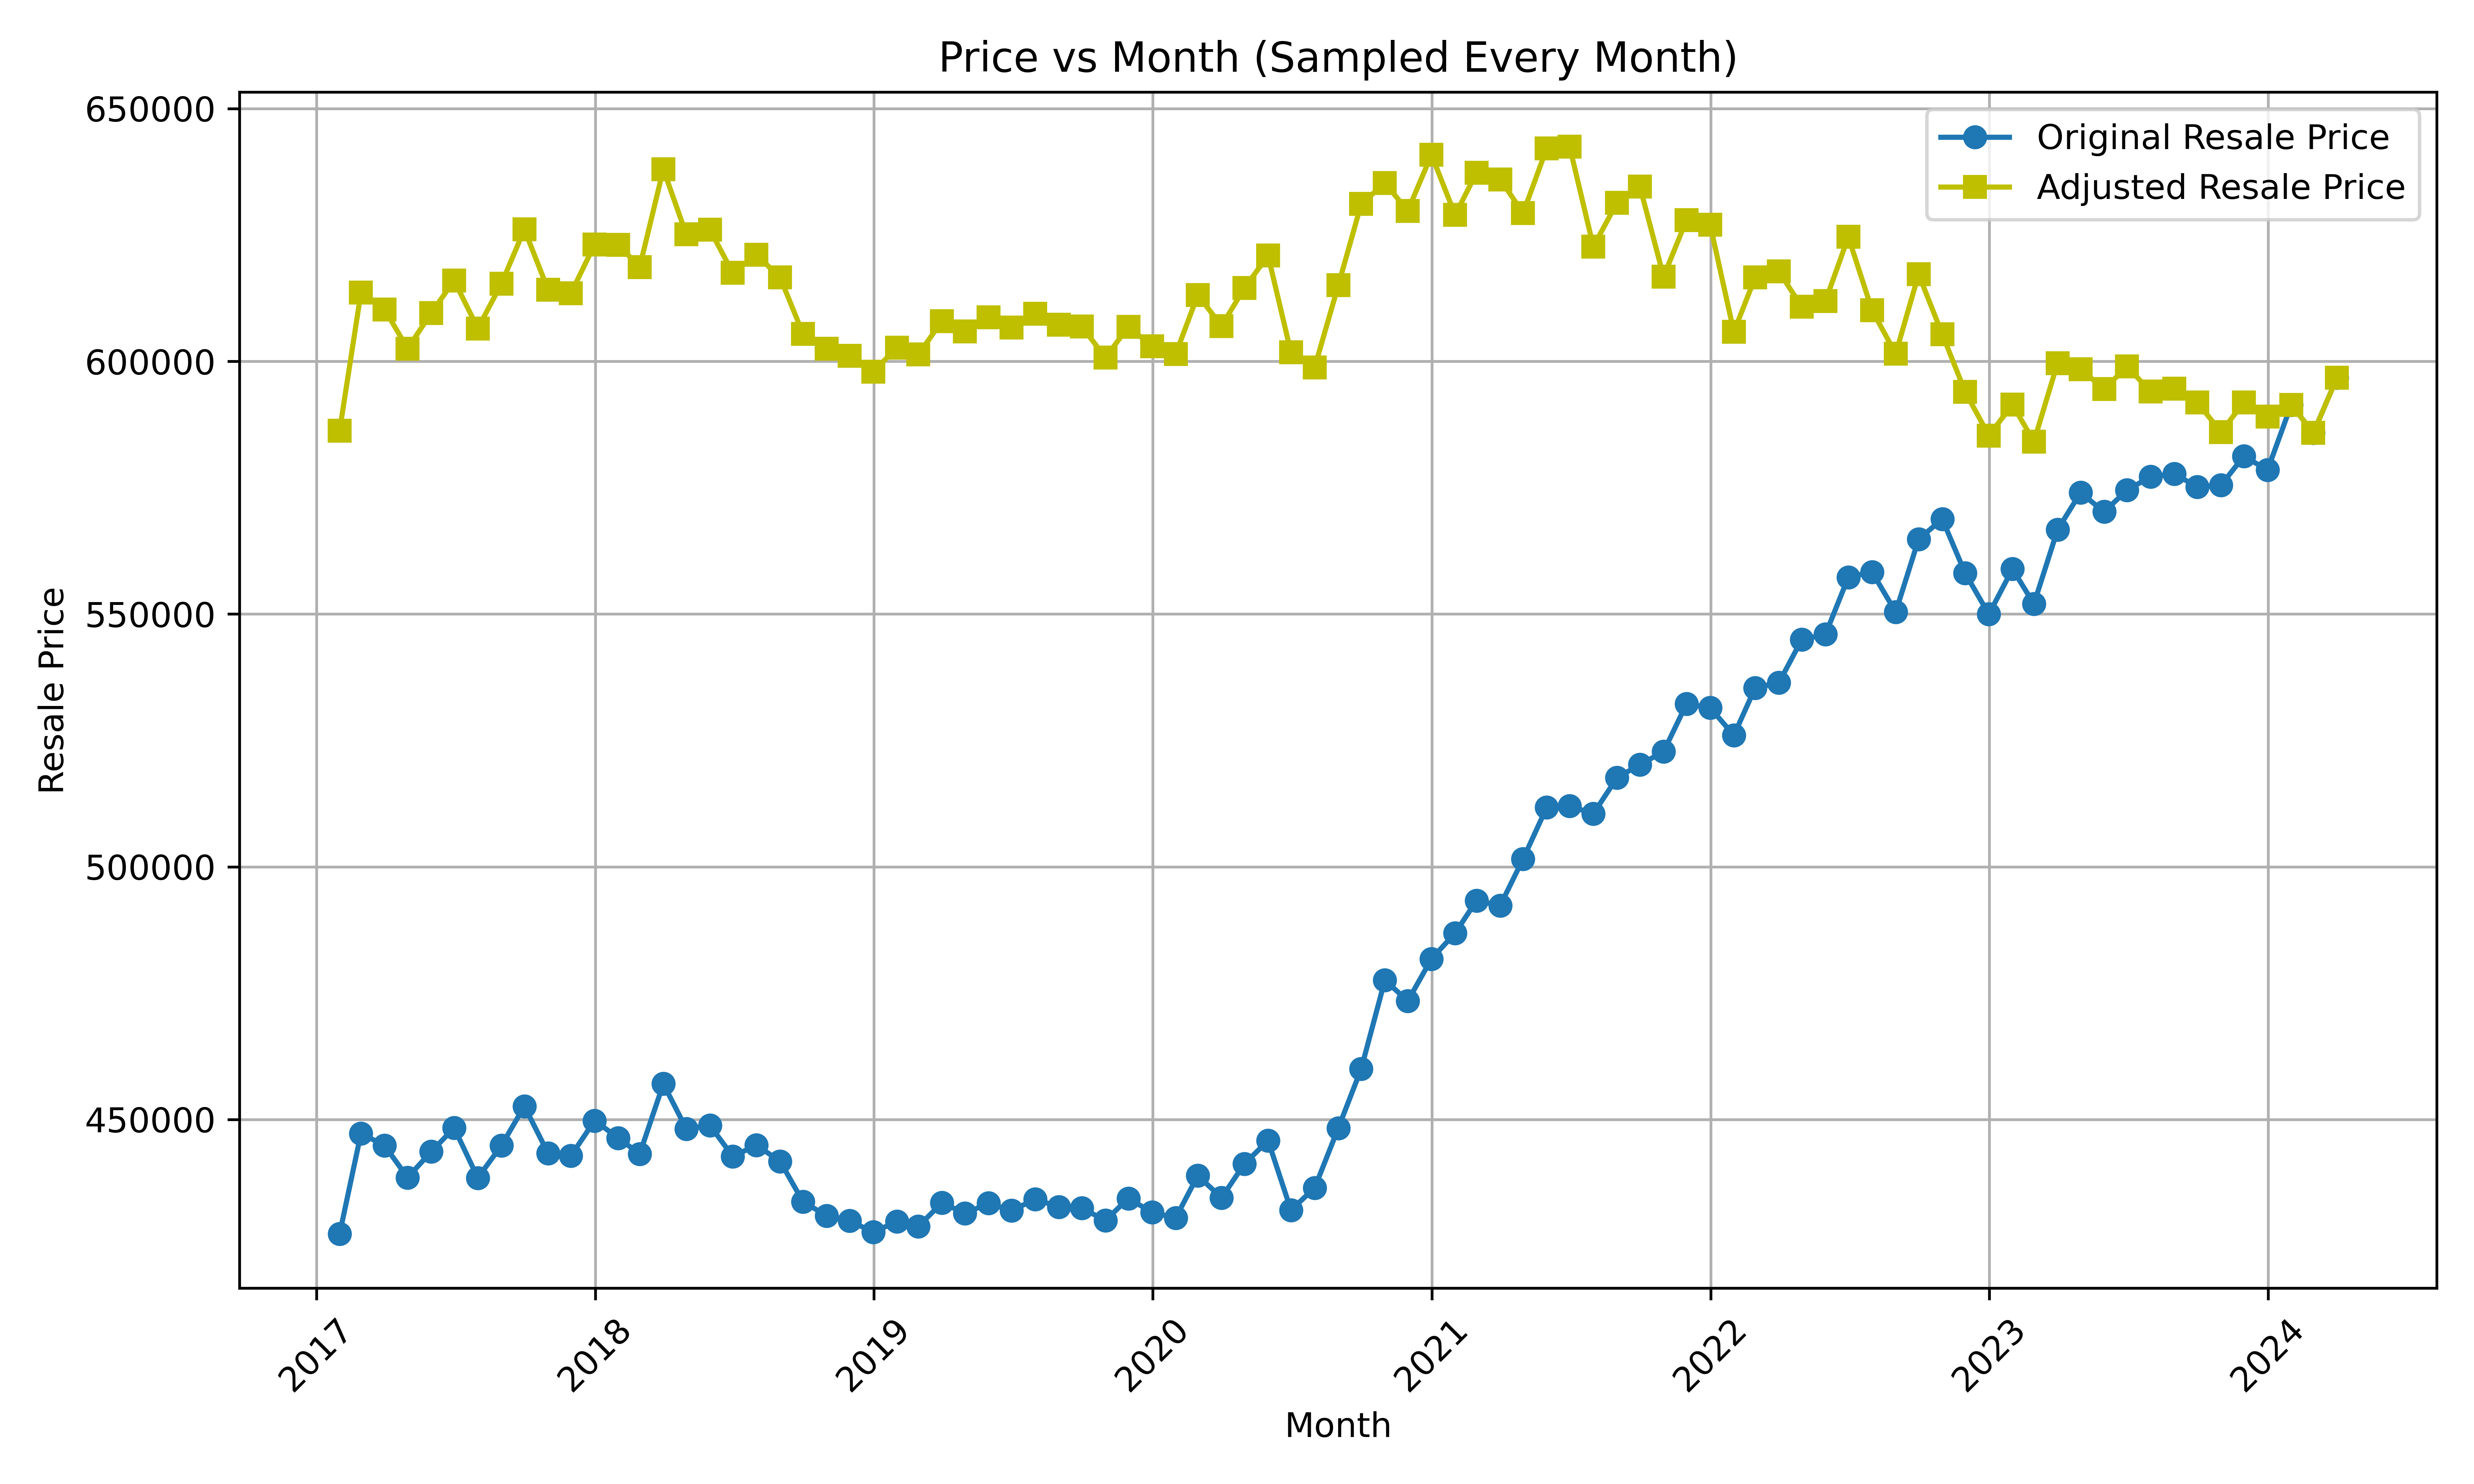
\includegraphics[width=0.75\textwidth]{imgs/adjusted_price.png}
\caption{Comparative illustration: Resale Price vs. Adjusted Price - Mitigating Inflationary Effects }\label{fig:priceinflation}
\end{figure}

Feature engineering ဆိုသည်မှာ မူလ dataset တွင် ပါ၀င်သည့် အချက်အလက်များကို မူတည်၍ အချက်အလက် အသစ်များ ဖန်တီးခြင်း၊ မူလ အချက်အလက်များကို machine learning မော်ဒယ် တည်ဆောက်ရာတွင် ပိုမို အဆင်ပြေစေရန် ပြုပြင်ခြင်းများကို ခေါ်သည်။ မူလ datasetတွင် တိုက်ခန်း၏ လက်ကျန်သက်တမ်း (\textit{\textbf{remaining lease}}) ကို ဖော်ပြရာ၌ ခုနှစ်နှင့်လ - ၂ ခုလုံးကို ဖော်ပြသည်။ အဆိုပါ အချက်အလက်ကို တွက်ချက်မှု ပြုလုပ်ရာတွင် လွယ်ကူစေရန်အတွက် စုစုပေါင်းလဖြင့် ဖော်ပြမည်။ ဥပမာ - သက်တမ်း ၄၁ နှစ် ၆ လ - ကျန်သည့် တိုက်၏ လက်ကျန်သက်တမ်းကို ဖော်ပြရာတွင် ၄၉၈ လ ဟု  လ အရည်အတွက်နှင့် ဖော်ပြသွားမည်။ 

အထက်ပါပုံတွင် တိုက်ခန်း၏ စျေးနှုန်းများကို လ အလိုက် နှိုင်းယှဥ်ကြည့်ရာ (အပြာရောင်လိုင်းဖြင့် ဖော်ပြထားသည်) တိုက်ခန်းများ၏ စျေးနှုန်းသည် အချိန်အလိုက် ပြောင်းလဲနေသည်ကို တွေ့ရမည်။ အထူးသဖြင့် ၂၀၂၁ နောက်ပိုင်း တွင် သိသိသာသာ စျေးနှုန်းများ ပြန်လည် မြင့်တက်လာသည်ကို တွေ့နိုင်သည်။ အဆိုပါ အချက်သည် အနာဂတ်တွင် ဖြစ်ပေါ်မည့် စျေးနှုန်းကို ခန့်မှန်းရာတွင် အသုံး၀င်သည့် အချက်ဖြစ်သော်လည်း တိုက်ခန်း၏ အခြားအချက်အလက်များဖြစ်သည့် အကျယ်အ၀န်း၊ တည်နေရာ စသည့် အချက်အလက်များကို မူတည်၍ စဥ်းစားရာတွင်မူ သတိထားရမည့် အချက် ဖြစ်လာသည်။ ဥပမာ -- ၂၀၂၃ တွင် ၅ သိန်း ၅ သောင်းနှင့် ရောင်းချခဲ့သည့် တိုက်ခန်းကို ၂၀၂၄ ခုနှစ် တွင် ရောင်းချမည်ဆိုပါက ၆ သိန်း နီးပါးဖြင့် ရောင်းချမည် ဖြစ်သည်။ သို့ဖြစ်ရာ တိုက်ခန်း၏ စျေးနှုန်းကို တွက်ချက်ရာတွင် မူလ ပေးထားသည့် စျေးနှုန်းအတိုင်း တိုက်ရိုက်တွက်ချက်ခြင်း မပြုဘဲ ၂၀၂၄ ခုနှစ်တွင် ဖြစ်ပေါ်မည့် ခန့်မှန်း စျေးနှုန်းကို မူတည်၍ စဥ်းစားသွားမည်။ ၂၀၂၄ ခုနှစ် ပထမ ၃ လ (ဇန်န၀ါရီမှ မတ်လ) အတွင်း ဖြစ်နိုင်သည့် စျေးနှုန်းကို သိရှိရန်အတွက်မူ Singapore အစိုးရမှ ထုတ်ပြန်ထားသည့် HDB resale price index ကို အသုံးပြု၍ ညှီမျှခြင်း \ref{eqn:adjusted_price}  တွင် ဖော်ပြထားသည့်အတိုင်း ခန့်မှန်းသွားမည် ဖြစ်သည်။ 

\subsubsection{Model Development: Build a Neural Network using Keras}
After data preprocessing, the clean dataset maintains its original size with 175,672 rows and now consists of 52 columns. The target variable is the \textit{\textbf{inflation-adjusted price}}, while the remaining 51 columns serve as features for training the neural network (deep learning) model. This section provides an explanation of each step in building the model. 

အထက်ပါ data preprocessing အဆင့်ဆင့်ကို ပြုလုပ်ပြီးနောက် dataset အသစ်တွင် အရောင်း စာရင်း အရေအတွက်မှာ မူလအတိုင်း တစ်သိန်း ခုနစ်သောင်း ငါးထောင် ခြောက်ရာ ခုနစ်ဆယ့် နှစ်ခု (၁၇၅,၆၇၂) ဖြစ်သော်လည်း column အရေအတွက်မှာမူ ၅၂ ခု အထိတိုးလာသည်။ inflation ကို ထည့်သွင်းစဥ်းစားထားသည့် စျေးနှုန်းကို Target အဖြစ်ထား၍ ခန့်မှန်းမည် ဖြစ်ပြီး ကျန် column ၅၁ ခု ကို Neural Network (deep learning model) ၏ input များ အဖြစ် အသုံးပြုမည်။ 

\begin{step} 
The project starts by importing the pandas library and loading a cleaned CSV file named \emph{\textbf{SGHDB2017-2024\_clean.csv}} into a Pandas DataFrame $df$. Then, the \emph{\textbf{adjusted\_price}} column, which represents the housing prices to be predicted, is extracted and stored in the variable $y$ and the remaining columns, which serve as features for the model, are stored in the variable $X$.

အဆင့် (၁) တွင် ဦးစွာ ပထမ  dataset အသစ် ကို Pandas DataFrame $df$ အဖြစ် သိမ်းဆည်းခြင်း ဖြစ်သည်။ ထို့နောက် အသုံးပြုမည့် Target ကို variable $y$ အဖြစ်လည်းကောင်း၊ ကျန် column များကို variable $X$ အဖြစ်လည်းကောင်း သိမ်းဆည်းမည်။ 

        \begin{lstlisting}
        # =========================================================================#
        import pandas as pd
        df = pd.read_csv('SGHDB2017-2024_clean.csv')
        y = df['adjusted_price'].values  
        X = df.drop(columns = 'adjusted_price')  
        # =========================================================================#
    \end{lstlisting}
\end{step}
\begin{remark}
    Ensure you have the necessary libraries installed. You can install them using pip if they are not already installed. For example: 
    \begin{lstlisting}
        pip install tensorflow pandas scikit-learn
    \end{lstlisting}
    သတိပြုရမည့် အချက်မှာ လိုအပ်သည့် library များကို  install ပြုလုပ်ရန် ဖြစ်သည်။ အကယ်၍ install မပြုလုပ်ရသေးပါက အထက်ပါ ကုဒ်ကို အသုံးပြု၍ install ပြုလုပ်ပေးရမည်။ 
\end{remark}

\begin{step}
This step prepares the data for building the machine learning model. 
\begin{itemize}
  \item The data is first split into training and testing sets, with 70\% of the data used for training (\(X_{\text{train}}\) and \(y_{\text{train}}\)) and 30\% for testing (\(X_{\text{test}}\) and \(y_{\text{test}}\)). The \texttt{random\_state=42} ensures reproducibility of the split.
  \item The continuous features are standardized using \texttt{StandardScaler}, which scales the data to have a mean of 0 and a standard deviation of 1. This transformation is applied separately to the training and testing sets to prevent data leakage. In this dataset, there are four continuous features: \texttt{flat\_type}, \texttt{floor\_area\_sqm}, \texttt{floor}, and \texttt{remaining\_lease\_months}.
  \item The scaled continuous features are combined with the binary features to form the final training (\(X_{\text{train}}\)) and testing (\(X_{\text{test}}\)) sets.
\end{itemize}

ဒုတိယ အဆင့်တွင် machine learning model တည်ဆောက်ရန် ဒေတာ အချက်အလက်များကို ပြင်ဆင်ရမည် ဖြစ်သည်။

ဦးစွာ ပထမ datasetကို training အတွက် ၇၀ ရာခိုင်နှုန်းကို အသုံးပြုပြီး ကျန် ၃၀ ရာခိုင်နှုန်းကို testing အတွက် ချန်ထားမည် ဖြစ်သည်။ ထို့နောက် continuous features များ ဖြစ်သည့် \texttt{flat\_type}၊ \texttt{floor\_area\_sqm}၊  \texttt{floor}, နှင့် \texttt{remaining\_lease\_months} များကို \texttt{StandardScaler} method ကို အသုံးပြု၍ range တစ်ခုအတွင်းရှိအောင် ပြုလုပ်ရမည်။ ထိုသို့ ပြုလုပ်ရာတွင် data leakage မဖြစ်စေရန် training နှင့် testing ဒေတာများကို သီးသန့်စီ ပြုလုပ်ရမည် ဖြစ်သည်။ 

\end{step}
\begin{lstlisting}
    # =========================================================================#
    import numpy as np
    from sklearn.preprocessing import StandardScaler
    from sklearn.model_selection import train_test_split
    # Step 2: Prepare the data
    X_train, X_test, y_train, y_test = train_test_split(X, y, test_size=0.3, random_state=42)

    # Standardize continuous features
    continuous_columns = ['flat_type', 'floor_area_sqm',  
                                   'floor', 'remaining_lease_months']
    binary_columns = df.columns.difference(continuous_columns 
                               + ['adjusted_price']).tolist()
    scaler = StandardScaler()
    X_train_continuous = scaler.fit_transform(X_train[continuous_columns])
    X_test_continuous = scaler.transform(X_test[continuous_columns])
    
    # Combine scaled continuous features and binary features
    X_train = np.hstack([X_train_continuous, X_train[binary_columns].values])
    X_test = np.hstack([X_test_continuous, X_test[binary_columns].values])
    # =========================================================================#
\end{lstlisting}  
\begin{step}
This step defines a function \texttt{create\_regression\_model} that constructs a feedforward neural network model for regression using TensorFlow's Keras API. 

တတိယ အဆင့်သည် TensorFlow ၏ Keras API ကို အသုံးပြု၍ neural network model တစ်ခု တည်ဆောက်ခြင်း ဖြစ်သည်။ ယခု model တွင် hidden layer - ၂ ခုသာ ပါ၀င်မည်ဖြစ်ပြီး ပထမ hidden layer တွင် neuron - ၃၂ ခု နှင့် ဒုတိယ hidden layer တွင် neuron -၁၆ ခု ကို အသုံးပြုမည်။ layer - ၂ ခုလုံးအတွက် ReLU activation function ကို အသုံးပြုထားသည်။ 

\begin{itemize}
    \item This function takes \texttt{input\_shape} as a parameter, representing the shape of the input data.
    \item Inside the function, a sequential model, as illustrated in Figure \ref{fig:mlp}, is created using \texttt{tf.keras.Sequential()}. 
    \item The model comprises an input layer, two hidden layers, and an output layer:
    \begin{itemize}
       \item The input layer serves as the initial receiver of input data, passing it to subsequent layers for processing.
       \item The first hidden layer is a fully connected (dense) layer with 32 units and ReLU activation function, as depicted in Figure \ref{fig:relu}.
       \item The second hidden layer is also fully connected, with 16 units and ReLU activation function.
       \item These hidden layers learn intricate patterns among the features.
       \item The output layer has a single unit, representing the regression prediction.
    \end{itemize}
    
    \item The code \texttt{model.compile(optimizer='adam', loss='mean\_squared\_error')} configures the neural network model. This project employs the \texttt{Adam} optimizer, an adaptive learning rate optimization algorithm. \texttt{Adam} adjusts the learning rate during training, facilitating faster convergence and improved performance. Additionally, \texttt{'mean\_squared\_error'} is used as the loss function, quantifying the difference between predicted and actual outputs during training.
\end{itemize}
\end{step}
\begin{lstlisting}
    # =========================================================================#
    import tensorflow as tf
    def create_regression_model(input_shape):
        model = tf.keras.Sequential([
            tf.keras.layers.InputLayer(shape=input_shape),        
            tf.keras.layers.Dense(32, activation='relu'),
            tf.keras.layers.Dense(16, activation='relu'),
            tf.keras.layers.Dense(1)
        ])    
        model.compile(optimizer='adam', loss='mean_squared_error')
    
        return model
        # =========================================================================#
\end{lstlisting}   
\begin{remark}
The size of hidden layers and the number of layers in a neural network are critical hyperparameters that influence the model's capacity, performance, and generalization ability. Finding the optimal configuration often involves a balance between model complexity and simplicity, guided by the specific characteristics of the dataset and the requirements of the task at hand. 

Hidden layer အရေအတွက်နှင့် neuron အရေအတွက်တို့မှာ neural network  တစ်ခုအတွက် အရေးကြီးသည့် hyperparameter များဖြစ်ပြီး dataset နှင့် ဖြေရှင်းမည့် ပြဿနာပေါ်တွင် မူတည်သည်။ 
\end{remark}

\begin{step}
The model is trained using the training data  (\(X_{\text{train}}\) and \(y_{\text{train}}\)). The training process runs for 10 epochs (Refer definition in Section \ref{def:epoch}) with a batch size of 32. 

အဆင့် (၄) တွင် training data များကို အသုံးပြု၍ အဆင့် (၃) တွင် တည်ဆောက်ခဲ့သည် neural network model ကို  train မည်ဖြစ်သည်။ ထိုသို့ train ရာတွင် ပြုလုပ်မည့် အကြိမ် အရေအတွက်ကို ၁၀ ဟု သတ်မှတ်ထားသည်။ ထို့အပြင် dataset ရှိ  data ပေါင်း တစ်သိန်းကျော်ကို တပြိုင်နက်ထဲ train ပြုလုပ်မည့် အစား တကြိမ်တွင် ဒေတာ (တိုက်ခန်းတစ်ခန်း၏ အရောင်းအ၀ယ် မှတ်တမ်း) - ၃၂ ခုကိုသာ အသုံးပြု၍  အကြိမ်ကြိမ် train ပြုလုပ်မည် ဖြစ်သည်။ ထိုသို့ ပြုလုပ်ခြင်းဖြင့် လိုအပ်သည့် memory နှင့် computational load  များကို လျော့ချနိုင်သည်။ 
    
\begin{lstlisting}
    # =========================================================================#
    model = create_regression_model(input_shape=[X_train.shape[1]])
    model.fit(X_train, y_train, epochs=10, batch_size=32, 
                    validation_data=(X_test, y_test))
    # =========================================================================#
\end{lstlisting}
\end{step}
\begin{remark}
Batch size refers to the number of training examples utilized in one iteration. Instead of using the entire dataset at once, training is divided into smaller batches. Using batch training allows for more efficient computation, as it reduces the memory requirements and computational load compared to processing the entire dataset at once.
\end{remark}

\begin{step}
In the last step, the model's performance is validated using the testing data (\(X_{\text{test}}\) and \(y_{\text{test}}\)) and saves the evaluation results to a CSV file.

နောက်ဆုံးအဆင့်တွင် model ၏ performance ကို testing ဒေတာများ အသုံးပြု၍ ဆန်းစစ်မည်။ 

\begin{lstlisting}
# Evaluate the model
from sklearn.metrics import mean_squared_error
from sklearn.metrics import mean_absolute_error, mean_absolute_percentage_error
from sklearn.metrics import r2_score

df_results = pd.DataFrame(columns=['Train', 'Test'])

y_pred = model.predict(X_train)
df_results.loc['Mean Squared Error', 'Train'] = mean_squared_error(y_train, y_pred)
df_results.loc['Mean Aboslute Error', 'Train'] = mean_absolute_error(y_train, y_pred)
df_results.loc['Mean Aboslute Percentage Error', 'Train'] = 
                        mean_absolute_percentage_error(y_train, y_pred)*100
df_results.loc['R2 score', 'Train'] = r2_score(y_train, y_pred)


y_pred = model.predict(X_test)
df_results.loc['Mean Squared Error', 'Test'] = mean_squared_error(y_test, y_pred)
df_results.loc['Mean Aboslute Error', 'Test'] = mean_absolute_error(y_test, y_pred)
df_results.loc['Mean Aboslute Percentage Error', 'Test'] = 
                        mean_absolute_percentage_error(y_test, y_pred)*100
df_results.loc['R2 score', 'Test'] = r2_score(y_test, y_pred)

df_results = df_results.round(2)
df_results.to_csv('model_evaluation.csv')
\end{lstlisting}
\end{step}

\subsubsection{Results and Discussion}
In this project, the model was trained without hyper-parameter tuning and subsequently evaluated on unseen test data to assess its efficacy. As illustrated in Table \ref{tab:results}, the model demonstrates robust predictive capability, with both the training and testing phases yielding results that closely align with actual values. 

The similarity in performance between the training and unseen data suggests that the model is not overfitting and is effectively generalizing to new instances. However, it's worth noting that an error of approximately SG\$65,000 may be deemed significant, particularly considering the average price of transactions in the training data, which is reported at SG\$611,563.8. This discrepancy represents roughly a 10\% deviation from the actual price, indicating room for further improvement in the model's precision.

ယခု သင်ခန်းစာတွင် ဖော်ပြထားသည့် model သည် hyper-parameter tuning  မပြုလုပ်ဘဲ တည်ဆောက်ထားသည့် model ဖြစ်သည်။  သို့သော် လက်ရှိ model၏ ရလဒ်မှာ သင့်တော် ကောင်းမွန်သည်ကို တွေ့ရသည်။ ခန့်မှန်း စျေးနှုန်းနှင့် မူလ စျေးနှုန်း၏ ပျမ်းမျှ ကွာခြားချက်သည် ခြောက်သောင်း ငါးထောင် ရှိပြီး တိုက်ခန်းများ၏ ပျမ်းမျှ ရောင်းစျေးနှုန်းနှင့် နှိုင်းယှဥ်ကြည့်ပါက ၁၀ ရာခိုင်နှုန်းလောက်သာ ကွာဟမှု ရှိသည်။ 

model ၏ hyper-parameter များဖြစ်သည့် hider layer များနှင့် neuron အရေအတွက်များကို တိုးမြှင့် အသုံးပြုမည်ဆိုပါက ပိုမိုကောင်းမွန်သည့် ရလဒ်များကို ရရှိနိုင်သည်။ 

\vspace{1em}

\begin{table}[htbp]
    \centering
    \caption{Model Evaluation Metrics}
    \label{tab:results}
    \begin{tabular}{l|r|r}
    \hline
    & \textbf{Train} & \textbf{Test} \\
    \hline
    Mean Squared Error & SG\$86,394.48 & SG\$86,284.83 \\
    Mean Absolute Error & SG\$65,017.51 & SG\$64,877.22 \\
    Mean Absolute Percentage Error & 10.82 \%& 10.82 \%\\
    R2 score & 82 \% & 82\% \\
    \hline
    \end{tabular}
\end{table}
\begin{remark}
The performance can be further enhanced by tuning the hyperparmeters, for instance, increasing the size of the hidden layers and depth of the neural network. 
\end{remark}
\newpage
\setcounter{stepcounter}{0}
\subsection{Multi-class Classification: Name Classification for Regional Identification} \label{sec:MMnames}
The objective of this project is to develop a machine learning model (neural network) specifically tailored to classify names to the corresponding states and regions within Myanmar. This model aims to address the challenges faced in demographic analysis and information extraction from news articles, where non-standardized writing of location names impedes accurate data interpretation.

အများသိကြသည့်အတိုင်း မြန်မာနိုင်ငံတွင် မူလက တိုင်းနှင့်ပြည်နယ် ၁၄ ခု ရှိခဲ့ပြီး ယခုအခါ နေပြည်တော် တိုးလာသည့်အတွက် ၁၅ ခု ရှိသည်။ ထို့အပြင် ရှမ်းကို ရှမ်း တောင်၊ ရှမ်းမြောက်နှင့် ရှမ်း ရှေ့ ဟူ၍ လည်းကောင်း၊ ပဲခူးကို ပဲခူအနောက်နှင့် ပဲခူး အရှေ့ဟု လည်းကောင်း ထပ်မံခွဲခြားထားရာ တိုင်းနှင့် ပြည်နယ် ၁၈ ခု ရှိသည်ကို ဆိုရမည်။ ဤ project ၏ ရည်ရွယ်ချက်မှာ နေရာတစ်ခု၏ အမည်ကို ပေးလိုက်သည်နှင့် မည်သည့် တိုင်းနှင့် ပြည်နယ်အတွင်း ရှိသည်ကို ခန့်မှန်းပေးရန် ဖြစ်သည်။ 

\subsubsection{Background}
In Myanmar, conducting social study research often involves collecting addresses from users, which can be challenging due to the lack of standardization in writing town and region names, particularly for smaller towns. Similarly, in news articles written by both local and international organizations, names are often written in non-standard ways, leading to inaccuracies in extracting location-based information. This project seeks to alleviate these challenges by automating the process of identifying the geographic origins associated with individual names.

မြန်မာ သတင်းအချက်အလက် စီမံခန့်ခွဲရေးအဖွဲ့ (MIMU)\cite{web:MIMU} ၏ ၏ ၂၀၁၉ ခုနှစ် ဒီဇင်ဘာလ စာရင်းအရ မြန်မာနိုင်ငံတွင် မြို့ပေါင်း ၄၆၉ မြို့နှင့် ကျေးရွာပေါင်း ၁၃,၅၉၀ ရှိသည်။ အဆိုပါ ကျေးရွာ အုပ်စုများ၏ အမည်များ နှင့် မြို့အမည်များကို စာလုံးပေါင်းဖော်ပြရာတွင် ဒေသအခေါ်အဝေါ်များနှင့် ကွဲလွဲမှုများ ရှိနေပါသည်။ ထို့အပြင် ထုတ်ပြန်ထားသည့် အမည်စာရင်းနှင့် ဒေသအခြေပြု သတင်းမီဒီယာများ၏ ဖော်ပြ ချက်များ အကြား ကွဲလွဲမှုများ ရှိနေပါသည်။ အဆိုပါကွဲလွဲမှုများကြောင့် လူမှုရေးနှင့် ဆိုင်သည့် သုတေသနေ လုပ်ငန်းများသည် နေရာ ဒေသအလိုက် အချက်အလက်များကို သုံးသပ်ရာတွင် တိကျမှု ရရှိနိုင်ရန် အခက်အခဲ များနှင့် ရင်ဆိုင် ကြုံတွေ့နေရသည်။ နေရာတစ်ခု၏ အမည်ကို ပေးလိုက်သည်နှင့် မည်သည့် တိုင်းနှင့် ပြည်နယ်အတွင်း ရှိသည်ကို အလွယ်တကူ ခန့်မှန်းပေးနိုင်မည့် Machine Learning Model တစ်ခု ကို တည်ဆောက်ထားခြင်းဖြင့် ပို၍ တိကျသည့် အချက်အလက်များကို သုံးသပ်နိုင်ရန် ရည်ရွယ်သည်။ 

\subsubsection{Dataset}
The initial datasets are obtained from the Myanmar Information Management Unit (MIMU) Resource Centre \cite{web:MIMU}, which offers comprehensive lists of names alongside their corresponding states and regions within Myanmar. The first dataset comprises 14,047 villages spread across 18 regions and states, while the second dataset includes 536 towns with their respective regions and states. These datasets serve as references for geographical information.

Additionally, supplementary data is collected from news articles, where variations in the spelling and formatting of town names are common. This dataset consists of 58,789 records spanning the same 18 regions and states. It's important to note that due to the nature of data collection from news articles, duplicate entries are present. Towns and regions are frequently mentioned in the articles, resulting in duplicated data instances.

Each dataset consists of two columns: 'state-region-names' and 'names of the location' (either villages or towns). Subsequently, these three datasets undergo comprehensive cleaning and merging processes to ensure coherence and consistency in the final combined dataset.

ဤ project တွင် အသုံးပြုမည့် dataset ကို မြန်မာ သတင်းအချက်အလက် စီမံခန့်ခွဲရေးအဖွဲ့ (MIMU) မှ ထုတ်နှုတ် ရယူထားခြင်း ဖြစ်သည်။ အဆိုပါ အဖွဲ့သည် မြန်မာနိုင်ငံရှိ ၀န်ကြီးဌာနအချို့နှင့် အဖွဲ့အစည်းများ၏ အချက်အလက်ကို စုစည်းတင်ပြထားသည့် ယုံကြည်စိတ်ချရသည့် အဖွဲ့အစည်းတစ်ခု ဖြစ်သည်။ ပထမ dataset တွင် ကျေးရွာပေါင်း  တစ်သောင်း လေးထာင် လေးဆယ့် ခုနစ် ခု ၏ အမည်များနှင့် အဆိုပါ မြို့ တည်ရှိသည့် တိုင်းနှင့်ပြည်နယ်၏ အမည်တို့ ပါ၀င်သည်။ ဒုတိယ dataset တွင်မူ မြို့ပေါင်း ၅၃၆ မြို့၏ အမည်များနှင့် သက်ဆိုင်ရာ တိုင်းနှင့်ပြည်နယ်၏ အမည်များ ပါ၀င်သည်။ ထို့အပြင် သတင်းခေါင်းစဥ်များမှ မြို့ရွာများ၏ အမည်များကို ထုတ်နှုတ်ရယူထားသည့် တတိယ dataset တွင် ငါးသောင်း ရှစ်ထောင် ခုနစ်ရာ ရှစ်ဆယ့်ကိုးခု ပါ၀င်သည်။ အထူးသတိပြုရမည့် အချက်မှာ ဤ တတိယ datasetသည် သတင်းများမှ အချက်အလက်များကို ထုတ်နှုတ် စုစည်းသည် ဖြစ်ရာ အချို့ မြို့များ၏ အမည်မှာ တစ်ကြိမ်မက ပါ၀င်နိုင်သည်။ 

dataset ၃ ခု လုံးတွင် column နှစ်ခု သာ ပါ၀င်ပြီး ပထမ column တွင် တိုင်းနှင့် ပြည်နယ်၏ အမည်များ ပါ၀င်သည်။ ဒုတိယ column တွင်မူ ကျေးရွာ(သို့မဟုတ်) မြို့၏ အမည်များ ပါ၀င်သည်။ 

\subsubsection{Data Preprocessing: Data Cleaning}
One of the major challenges in this project is name consistency, even for the names of the regions and states. For instance, the regions and states in the MIMU dataset are defined as "shan (south)," but in the news articles, they are usually defined as "shan-south." This inconsistency necessitates intensive data cleaning to ensure uniformity across datasets.

\begin{itemize}
  \item \textbf{Standardizing Column Names}: The column names of three datasets are standardized to ensure consistency. Specifically, the columns representing the names of regions and states are renamed to `SR\_Name' for uniformity across datasets.
  \item \textbf{Standardizing Naming Convention}:Fuzzy string matching techniques are employed to address variations in naming conventions between datasets. Specifically, the names in the news articles dataset are compared to the standardized names in the MIMU dataset, and the closest matches are identified and used to replace inconsistent names.
  \item \textbf{Removing Duplicates}: Duplicate rows in the news articles dataset are removed to enhance data quality and reduce redundancy.
  \item \textbf{Merging} The cleaned and standardized datasets are combined to form a comprehensive dataset (df\_mimu), consolidating information from both the MIMU dataset and news articles. This merged dataset encompasses 19,513 entries across 2 columns, enabling seamless progression to further analysis and modeling.
\end{itemize}

မြန်မာ သတင်းအချက်အလက် စီမံခန့်ခွဲရေးအဖွဲ့ (MIMU) မှ ရယူထားသည့် dataset တွင် ရှမ်း (တောင်)၊ ရှမ်း (မြောက်) - စသည်ဖြင့် တောင်နှင့် မြောက်ကို ကွင်းစ ကွင်းပိတ်နှင့် အသုံးပြု ဖော်ပြထားသော်လည်း သတင်းဌာနမှ ရယူထားသော ပြည်နည် အမည်များတွင်မူ ရှမ်း -တောင်၊  ရှမ်း -မြောက် စသည်ဖြင့် `-' ကို အသုံးပြု ထားသည်။ အဆိုပါ အမည် သတ်မှတ်ချက်များကို ကိုက်ညီစေရန် အတွက် Fuzzy string matching ကို အသုံးပြုသည်။ ထို့အပြင် သတင်းဌာနမှ ရယူထားသည့် dataset ထပ်နေသည့် မြို့အမည်၊ ကျေးရွာအမည်များကို ဖယ်ထုတ်သည်။ ထို့နောက် dataset ၃ ခု လုံးကို တစ်စုတည်းပေါင်းစည်းလိုက်ပြီး စုပေါင်း dataset တွင် record စုစုပေါင်း -- တစ်သောင်း ကိုးထောင် ငါးရာ တစ်ဆယ့်သုံးခုနှင့် column နှစ်ခု ပါ၀င်သည်။ 

\subsubsection{Data Preprocessing: Text Encoding (Vectorization)}

In this step, the text inputs from the 'name' column and the class labels from the 'SR\_Name' column are transformed into numerical representations. This transformation is necessary to convert the textual data into a format that can be processed by a neural network. 

\begin{itemize}
  \item Label encoding is applied on the `SR\_Name' column to map each unique stage/region name to a numerical value. Label encoding assigns a unique integer label to each unique category in the column.
  \item One-hot encoding is applied to the 'name' column because each name represents a specific location, and there is no ordinal relationship between the different names. This encoding method transforms categorical variables into binary vectors, where each unique category (name) is represented by a binary feature. This results in a sparse matrix with 13,003 binary columns, each representing a distinct name.
\end{itemize}

ဤ dataset တွင် ပါ၀င်သည့် အချက်အလက်များမှာ စာသားများဖြင့် ဖော်ြပ ထားသည် ဖြစ်ရာ ကိန်းဂဏန်းများ အဖြစ် ဦးစွာပြောင်းလဲမည်။ တိုင်းနှင့်ပြည်နယ်များ၏ အမည်များပါ၀င်သော `SR\_Name' column ကို Label encoding အသုံးပြု၍ ကိန်းဂဏန်းများအဖြစ် တိုက်ရိုက် ပြောင်းလဲမည်။ ဥပမာ -- ရှမ်း (တောင်) ကို ၁၅ ၊ ရခိုင်ကို ၁၂  ၊ ဧရာ၀တီကို သုည စသည်ဖြင့် သတ်မှတ်သည်။ ထို့နောက် ကျေးရွာအုပ်စုများနှင့် မြို့များ၏ အမည်ကို One-hot encoding နည်းစနစ်ကို အသုံးပြု၍ Binary Column များအဖြစ် ပြောင်းလဲမည်။ ဤ dataset တွင် ကျေးရွာအုပ်စုများနှင့် မြို့များ၏ အမည် စုစုပေါင်း တစ်သောင်း သုံးထောင် သုံးခု ပါ၀င်ရာ dataset ၏ record (row) တစ်ခုစီကို ($1 \times 13,003$) binary array များဖြင့် ဖော်ပြသွားမည်။ 

\subsubsection{Model Development: Build a Neural Network using Keras}
With the merged dataset containing 19,513 entries across 2 columns, the second column `name' of the location is used as an input feature and the first column `SR\_Name' is the class label (output) for the model. The section explains the steps for developing a neural network model using Keras for classifying the text inputs to 18 different regions and stages.  

%------step 1------
\begin{step} 
The first step in our data processing pipeline involves loading the data into a pandas DataFrame. This is accomplished using the pandas library, which is imported at the beginning of the script.

အဆင့် (၁) တွင် ဦးစွာ ပထမ  dataset ကို Pandas DataFrame $df$ အဖြစ် သိမ်းဆည်းခြင်း ဖြစ်သည်။ 

\begin{lstlisting}
# =========================================================================#
# Step 1: Load the data
import pandas as pd
df = pd.read_csv('./data/MMNames_clean.csv')
# =========================================================================#
\end{lstlisting}
\end{step}
\begin{remark}
    Ensure you have the necessary libraries installed. You can install them using pip if they are not already installed. For example: 
    \begin{lstlisting}
        pip install tensorflow pandas scikit-learn
    \end{lstlisting}
    သတိပြုရမည့် အချက်မှာ လိုအပ်သည့် library များကို  install ပြုလုပ်ရန် ဖြစ်သည်။ အကယ်၍ install မပြုလုပ်ရသေးပါက အထက်ပါ ကုဒ်ကို အသုံးပြု၍ install ပြုလုပ်ပေးရမည်။ 
\end{remark}
%------step 2-----
\begin{step}
This step prepares the data for building the machine learning model. This step involves preprocessing the data to get it ready for training a machine learning model. The code uses custom preprocessing functions in user-defined module `data\_preprocessing' and utilities from the sklearn library to achieve this.
\begin{itemize}
  \item The first three lines of the code below import the user-defined module `data\_preprocessing' and utilities from the sklearn library. 
  
  \item The code 'dp.preprocess\_category(df, 'SR\_Name')' preprocesses the \texttt{`SR\_Name'} column of the DataFrame df using label encoding. This method converts categorical values to numerical values, facilitating their use in machine learning algorithms.
  
  \item The code 'dp.preprocess\_category(df, 'name')'encodes the name column of the DataFrame df into a binary matrix representation using one-hot encoding. This technique enhances the model's ability to interpret and utilize categorical data effectively. 
      
  \item The preprocessed data is then split into training and testing sets, with 70\% of the data used for training (\(X_{\text{train}}\) and \(y_{\text{train}}\)) and 30\% for testing (\(X_{\text{test}}\) and \(y_{\text{test}}\)). The \texttt{random\_state=42} ensures reproducibility of the split.
\end{itemize}

ဒုတိယ အဆင့်တွင် machine learning model တည်ဆောက်ရန် ဒေတာ အချက်အလက်များကို ပြင်ဆင်ရမည် ဖြစ်သည်။ အောက်တွင် ပေးထားသော ကုဒ်၏ ပထမ ၃ ကြောင်းမှာ လိုအပ်သည့် module များကို import လုပ်ခြင်းဖြစ်သည်။ ထို့နောက် 'dp.preprocess\_category(df, 'SR\_Name')' ကုဒ်သည် `SR\_Name' column ကို Label encoding အသုံးပြု၍ ကိန်းဂဏန်းများအဖြစ် တိုက်ရိုက် ပြောင်းလဲခြင်းဖြစ်ပြီး 'dp.preprocess\_category(df, 'name')'သည်  ကျေးရွာအုပ်စုများနှင့် မြို့များ၏ အမည်ကို One-hot encoding နည်းစနစ်ကို အသုံးပြု၍ Binary Column များအဖြစ် ပြောင်းလဲပေးသည်။  ထို့နောက် datasetကို training အတွက် ၇၀ ရာခိုင်နှုန်းကို အသုံးပြုပြီး ကျန် ၃၀ ရာခိုင်နှုန်းကို testing အတွက် ချန်ထားမည် ဖြစ်သည်။ 
\end{step}
\begin{lstlisting}
# =========================================================================#
# Step 2: Prepare the data
import data_preprocessing as dp
from sklearn.preprocessing import StandardScaler
from sklearn.model_selection import train_test_split

df = dp.preprocess_category(df,'SR_Name')
df = dp.preprocess_onehot(df,'name')

y = df['SR_Name'].values 
X = df.drop(columns=['SR_Name']).values

X_train, X_test, y_train, y_test = train_test_split(X, y, test_size=0.3, random_state=42)
print(X_train.shape, X_test.shape)
# =========================================================================#
\end{lstlisting}
%-- step 3---
\begin{step}
This step defines a function \texttt{create\_regression\_model} that constructs a feedforward neural network model for classification using TensorFlow's Keras API. 

တတိယ အဆင့်သည် TensorFlow ၏ Keras API ကို အသုံးပြု၍ neural network model တစ်ခု တည်ဆောက်ခြင်း ဖြစ်သည်။ ယခု model တွင် hidden layer - ၂ ခုသာ ပါ၀င်မည်ဖြစ်ပြီး ပထမ hidden layer တွင် neuron - ၃၂ ခု နှင့် ဒုတိယ hidden layer တွင် neuron -၁၆ ခု ကို အသုံးပြုမည်။ layer - ၂ ခုလုံးအတွက် ReLU activation function ကို အသုံးပြုထားသည်။ 

\begin{itemize}
    \item This function takes \texttt{input\_shape} and \texttt{num\_classes} as parameters, representing the shape of the input data and the number of classes.
    \item The model comprises an input layer, two hidden layers, and an output layer:
    \begin{itemize}
       \item The input layer serves as the initial receiver of input data, passing it to subsequent layers for processing.
       \item The first hidden layer is a fully connected (dense) layer with 32 units and \texttt{ReLU} activation function, as depicted in Figure \ref{fig:relu}.
       \item The second hidden layer is also fully connected, with 16 units and \texttt{ReLU} activation function.
       \item These hidden layers learn intricate patterns among the features.
       \item The output layer has a single unit, representing the classification prediction. The \texttt{`softmax'} activation function is used in the output layer.
    \end{itemize}
    
    \item The code \texttt{model.compile(optimizer='adam', loss='sparse\_categorical\_crossentropy', metrics=['accuracy'])} configures the neural network model. 
    \item This project employs the \texttt{Adam} optimizer, an adaptive learning rate optimization algorithm. \texttt{Adam} adjusts the learning rate during training, facilitating faster convergence and improved performance. 
    \item The loss function \texttt{'sparse\_categorical\_crossentropy'}loss function is utilized, which calculates the cross-entropy loss between the predicted probabilities and the true labels. This loss function is suitable for multi-class classification tasks where the target labels are integers.
    \item The \texttt{`accuracy'} metric is selected to evaluate the model's performance. It measures the proportion of correctly classified samples out of the total number of samples, providing a straightforward assessment of the model's predictive accuracy.
\end{itemize}
\end{step}

\begin{lstlisting}
# =========================================================================#
import tensorflow as tf

def create_classification_model(input_shape, num_classes, params={}):
    model = tf.keras.Sequential([
        tf.keras.layers.InputLayer(shape=input_shape),
        tf.keras.layers.Dense(32, activation='relu'),
        tf.keras.layers.Dense(16, activation='relu'),
        tf.keras.layers.Dense(num_classes, activation='softmax')
    ])

    model.compile(optimizer='adam', 
                loss='sparse_categorical_crossentropy', metrics=['accuracy'])
    
    return model
     # =========================================================================#
\end{lstlisting}   
\begin{remark}
The size of hidden layers and the number of layers in a neural network are critical hyperparameters that influence the model's capacity, performance, and generalization ability. Finding the optimal configuration often involves a balance between model complexity and simplicity, guided by the specific characteristics of the dataset and the requirements of the task at hand. 

Hidden layer အရေအတွက်နှင့် neuron အရေအတွက်တို့မှာ neural network  တစ်ခုအတွက် အရေးကြီးသည့် hyperparameter များဖြစ်ပြီး dataset နှင့် ဖြေရှင်းမည့် ပြဿနာပေါ်တွင် မူတည်သည်။ 

\end{remark}
% step 4 ----
\begin{step}
The model is trained using the training data  (\(X_{\text{train}}\) and \(y_{\text{train}}\)). The training process runs for 10 epochs (Refer definition in Section \ref{def:epoch}) with a batch size of 32. 

အဆင့် (၄) တွင် training data များကို အသုံးပြု၍ အဆင့် (၃) တွင် တည်ဆောက်ခဲ့သည် neural network model ကို  train မည်ဖြစ်သည်။ ထိုသို့ train ရာတွင် ပြုလုပ်မည့် အကြိမ် အရေအတွက်ကို ၅၀ ဟု သတ်မှတ်ထားသည်။ ထို့အပြင် dataset ရှိ  data ပေါင်း တစ်သိန်းကျော်ကို တပြိုင်နက်ထဲ train ပြုလုပ်မည့် အစား တကြိမ်တွင် ဒေတာ - ၃၂ ခုကိုသာ အသုံးပြု၍  အကြိမ်ကြိမ် train ပြုလုပ်မည် ဖြစ်သည်။ ထိုသို့ ပြုလုပ်ခြင်းဖြင့် လိုအပ်သည့် memory နှင့် computational load  များကို လျော့ချနိုင်သည်။ 
    
\begin{lstlisting}
    # =========================================================================#
    model = create_classification_model(input_shape=[X_train.shape[1]],
                num_classes=len(df['SR_Name'].unique()), )
    history = model.fit(X_train, y_train, epochs=50, batch_size=32, 
                validation_data=(X_test, y_test), verbose=0)
    # =========================================================================#
\end{lstlisting}
\end{step}
\begin{remark}
Batch size refers to the number of training examples utilized in one iteration. Instead of using the entire dataset at once, training is divided into smaller batches. Using batch training allows for more efficient computation, as it reduces the memory requirements and computational load compared to processing the entire dataset at once.
\end{remark}

% ----step 5 ----

\begin{step}
In the last step, the model's performance is validated using the testing data (\(X_{\text{test}}\) and \(y_{\text{test}}\)) and saves the evaluation results to a CSV file. In this step, the \texttt{`classification\_report'} function from scikit-learn is used to generate a classification report for the actual test labels (\texttt{y\_test}) and the predicted labels (\texttt{y\_pred}).

နောက်ဆုံးအဆင့်တွင် model ၏ performance ကို testing ဒေတာများ အသုံးပြု၍ ဆန်းစစ်မည်။ 

\begin{lstlisting}
# Step 5: Evaluate the model

from sklearn.metrics import classification_report

y_pred = model.predict(X_test, batch_size=32, verbose=0)
y_pred = y_pred.argmax(axis=1)
report = classification_report(y_test, y_pred, output_dict=True)
report_df = pd.DataFrame(report).transpose()
report_df.to_csv('./data/cls_report_test.csv', index=False)
print(report_df)
y_pred = model.predict(X_train, batch_size=32, verbose=0)
y_pred = y_pred.argmax(axis=1)
report = classification_report(y_train, y_pred, output_dict=True)
report_df = pd.DataFrame(report).transpose()
report_df.to_csv('./data/cls_report_train.csv', index=False)

\end{lstlisting}
\end{step}

\subsubsection{Results and Discussion}
\begin{table}[htbp]
    \centering
    \caption{Model Evaluation Metrics}
    \label{tab:P2results}
    \begin{tabular}{l|r|r}
    \hline
    & \textbf{Train} & \textbf{Test} \\
    \hline
    Accuracy                            & 86\% & 28\% \\
    weighted average Precision & 87\% & 45\% \\
    weighted average Recall      & 86\% & 28\%\\
    \hline
    \end{tabular}
\end{table}

In the results presented above (Ref. Table \ref{tab:P2results}), it's evident that while the model attained an accuracy of 86\% on the training data, it only achieved 28\% on the test data. Similarly, the model demonstrated weighted average precision and recall rates of 87\% and 86\% on the training set, but notably dropped to 45\% and 28\% on the test set. These findings indicate that the developed neural network model, a fully connected multi-layer perceptron, isn't well-suited for this particular problem. Its overfitting can be attributed to its inability to capture sequential patterns and inherent relationships within textual data, such as location names. Such limitations often lead to poor generalization to new data, particularly when dealing with high-dimensional sparse datasets like one-hot encoded vectors.

This is where more advanced models, such as Recurrent Neural Networks (RNNs), come into play. RNNs are designed to recognize sequential patterns and dependencies in data by maintaining a hidden state that captures information from previous time steps. This makes RNNs particularly effective for tasks involving sequential data, such as natural language processing, where understanding the order and context of words (or characters) is crucial. 

%However, in this particular problem, a simpler model like Bernoulli Naive Bayes provides good performance, with an accuracy score of 0.78 for the testing set and 0.86 for the training set. This demonstrates that while neural networks are powerful, they might not always be necessary or the best choice for every classification problem.

In the next chapter, we will delve into the advanced deep learning models, particularly one particular section focusing on Recurrent Neural Networks (RNNs). We will explore their design principles, operational mechanisms, and why they are better suited for handling sequential data in tasks like sentiment analysis. 

အထက်ပါ ဇယားတွင် ဖော်ပြထားသည့် ရလဒ်များကို သုံးသပ်ကြည့်မည်ဆိုပါက ယခု သင်ခန်းစာတွင် တင်ပြထားသည့် neural network model (fully connected multi-layer perceptron) သည် အမည်များကို မှန်မှန်ကန်ကန် ခွဲခြားပေးနိုင်ခြင်း မရှိသည်ကို တွေ့ရသည်။ train ပြုလုပ်ထားသည့် data အတွက် ၈၆ ရာခိုင်နှုန်းလောက်ထိ ကောင်းမွန် တိကျသည့် ရလဒ်များကို ထုတ်ပေးနိုင်သော်လည်း အသစ် data များအတွက်မူ ၄င် model ၏ ရလဒ်မှာ ၅၀ ရာခိုင်နှုန်းအောက် ကျဆင်းသွားသည်။ Text data များကို အမျိုးအစား ခွဲခြားကြရာတွင် အများဆုံး အသုံးပြုသည့်  model မှာ  Recurrent Neural Networks (RNNs) ဖြစ်သည်။ အထူးသဖြင့် စကားလုံး တစ်လုံးမက ပါ၀င်သည့် စာကြောင်းများကို အမျိုးအစားခွဲခြားသည့် sentiment analysis ကဲ့ သို့ ပြဿနာများတွင် RNN ၏ စွမ်းဆောင်ရည်မှာ ပိုမိုကောင်းမွန်ကြောင်း သုတေသနပညာရှင်များက သက်သေပြခဲ့ပြီး ဖြစ်သည်။ 

%သို့သော် စကားလုံး တစ်လုံး ၊ နှစ်လုံးသာ ပါ၀င်သည့် ယခု ပြဿနာတွင်မူ ရိုးရှင်းလွယ်ကူသည့် Bernoulli Naive Bayes machine learning model ကို အသုံးပြုခြင်းဖြင့် ပို၍ ကောင်းမွန်သည့် ရလဒ်များ ရရှိသည်ကို တွေ့ရသည်။ neural networks (သို့မဟုတ်) deep learning model များသည် ယေဘူယျအားဖြင့် ပိုမိုကောင်းမွန်သည့် ရလဒ်များကို ပေးနိုင်သည်ဟု ဆိုသော်လည်း ပြဿနာတိုင်းအတွက် မဟုတ်သည်ကို သတိပြုသင့်သည်။  

နောက် အခန်းတွင် RNN အပါအ၀င် advanced deep learning model များကို ဆွေးနွေးသွားမည်။ 

\newpage

\section{Chapter-End Exercises}\label{sec:exercises}

This section provides chapter-end exercises aimed at reinforcing learning and assessing comprehension of the foundation of the neural network, activation function, forward propagation and backward propagation. Readers are encouraged to attempt these exercises independently prior to checking solutions.

\begin{question}
You have a neural network model with one hidden layer, as shown in Figure \ref{fig:Ex2-1}. The input data point has two features: $x_1=1$ and $x_2 = 1$. The ReLU activation function is used in the hidden layer, resulting in: $h_1 = 6$ and $h_2=0$ for the hidden layer outputs. The weights on the edges connecting the hidden and output layer are -1 and 1, respectively. What prediction ($y$) would this model make on this data point? Assume that the output layer uses the sigmoid function.
\end{question} 

\vspace{0.5em}
\begin{figure}[h]%
\centering
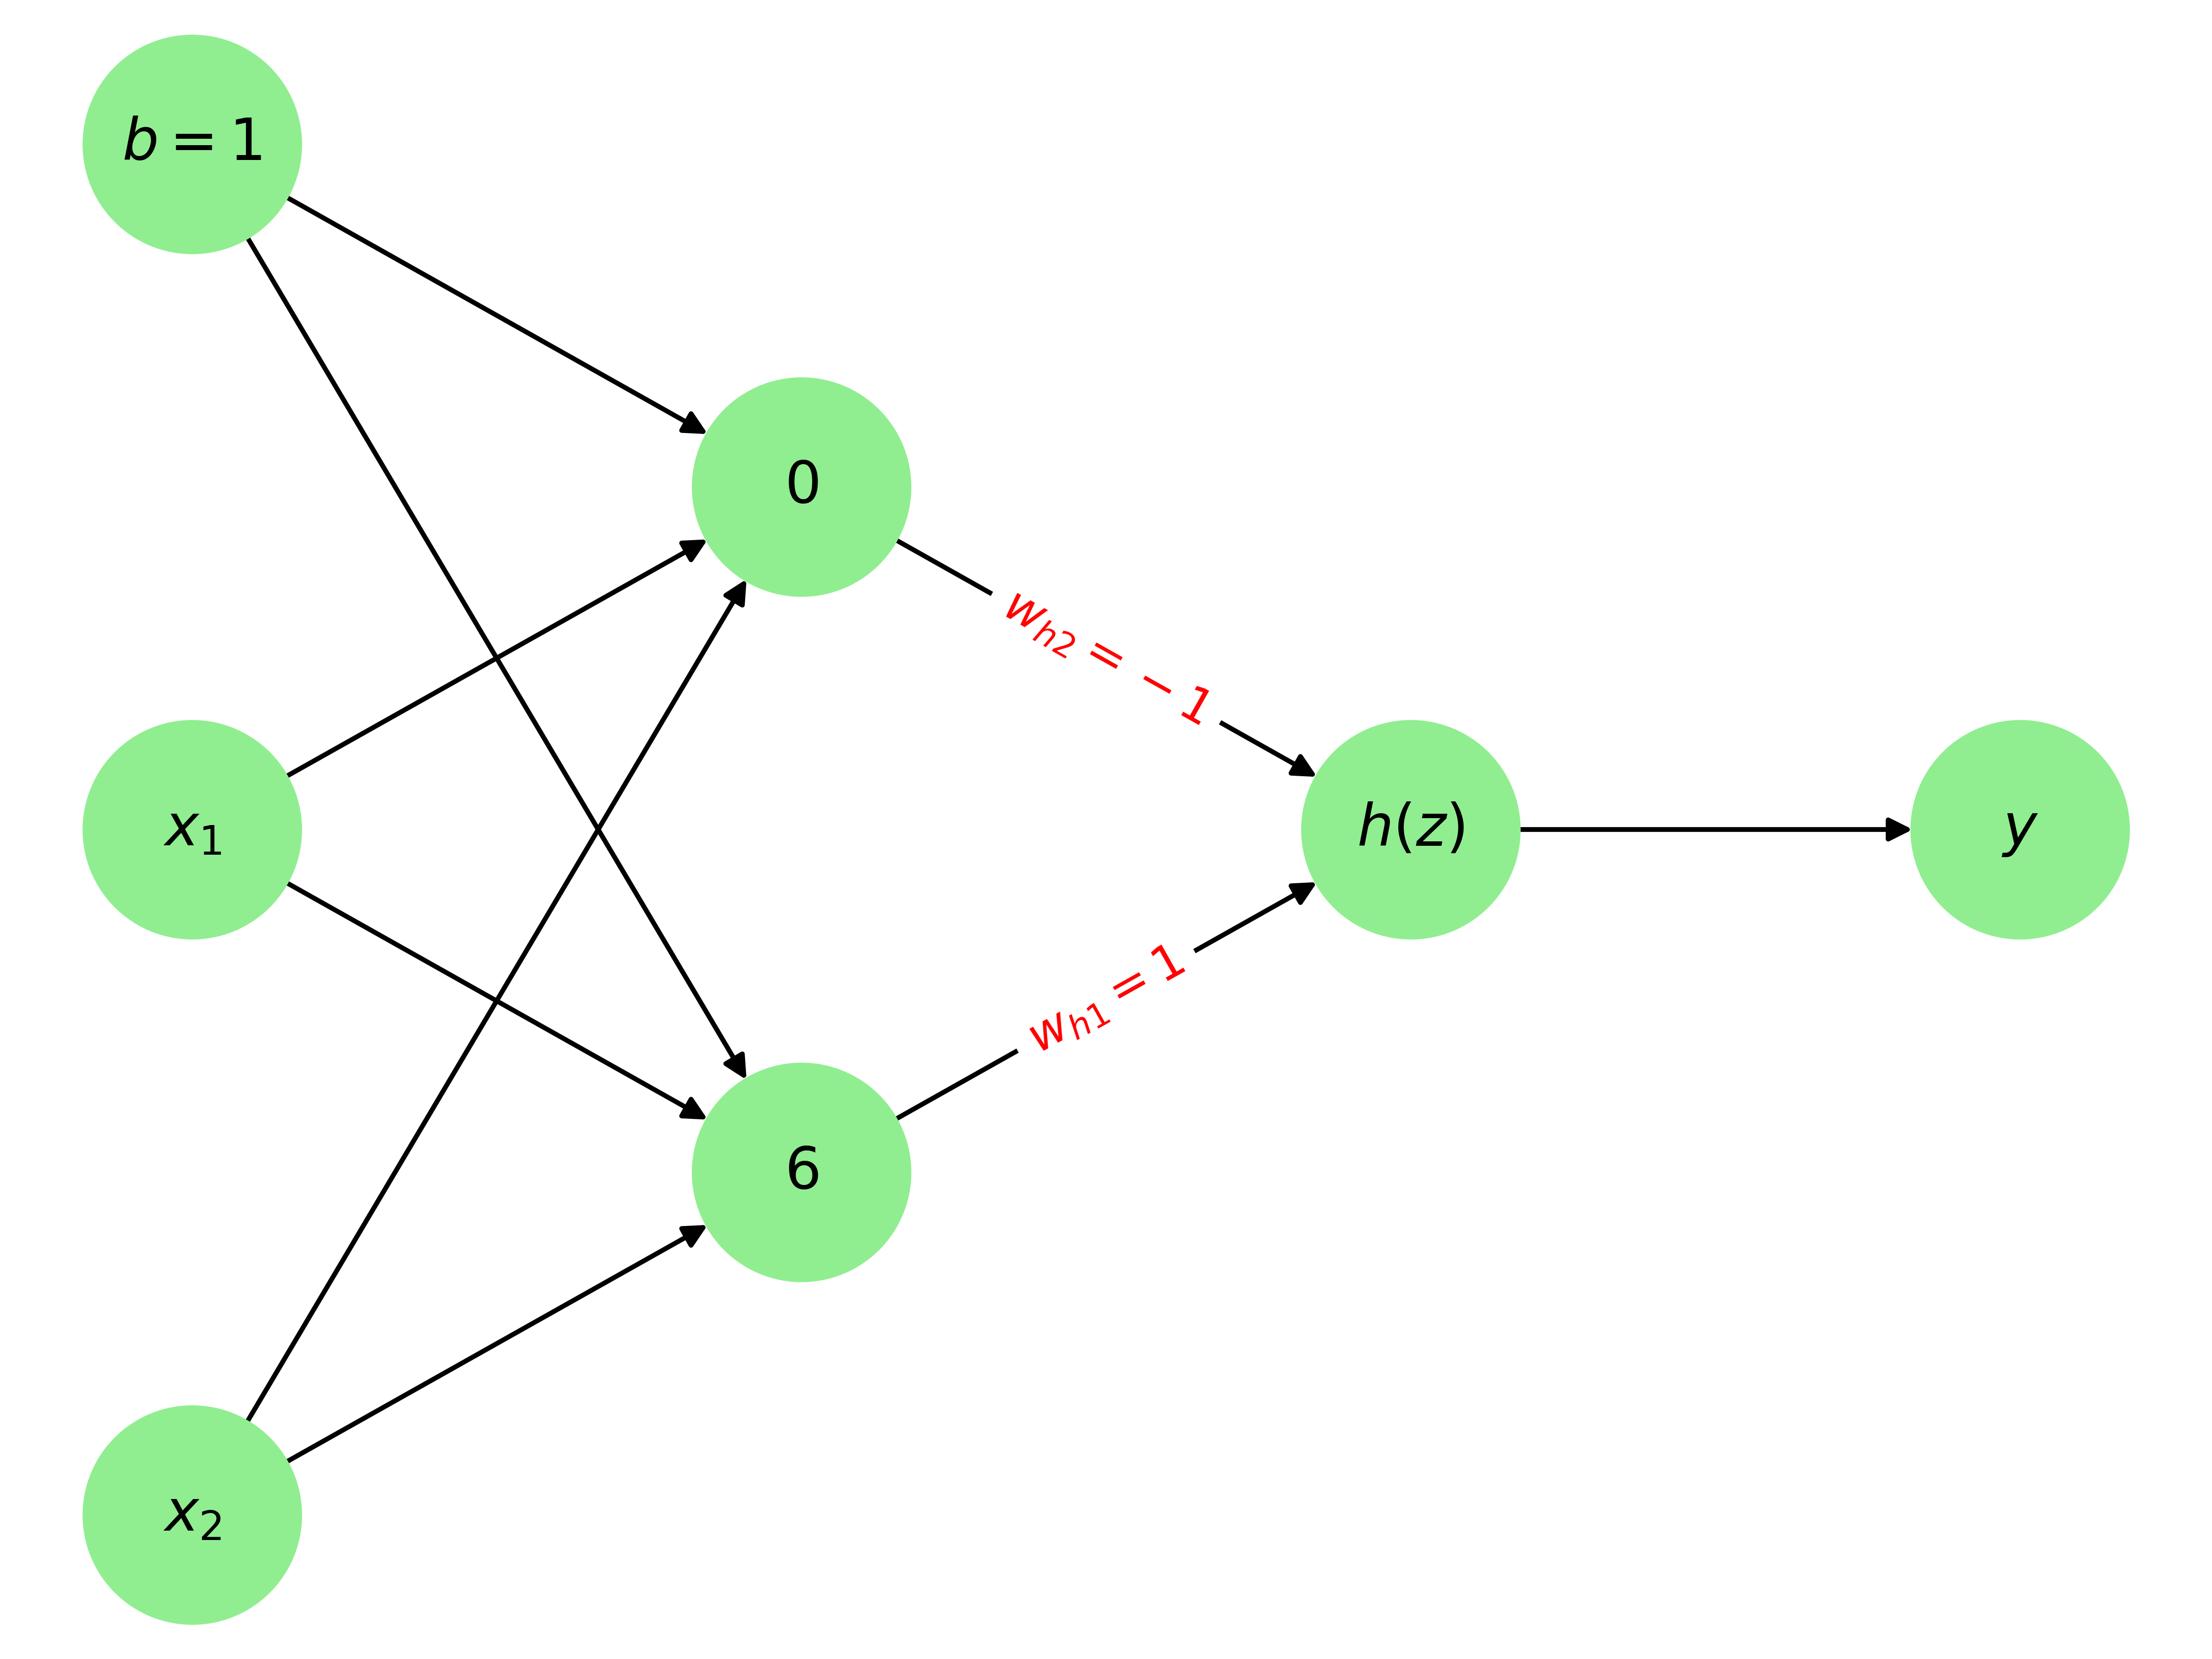
\includegraphics[width=0.675\textwidth]{imgs/chap2_ex1.png}
\caption{Forward Propagation in a NN with two hidden layers}\label{fig:Ex2-1}
\end{figure}

\begin{answer}
The weighted sum of the inputs to the output layer can be calculated as: 
\begin{equation}\label{eq:ex1}
  z = \omega_{h1}*h_1 + \omega_{h2}*h_2 = (1)*6 + (-1)*0 = 6
\end{equation} Then, applying the sigmoid activation function: the value of
\begin{equation}\label{eq:ex1}
  y = \frac{1}{1+\exp{(-6)}} = 0.997
\end{equation}
\end{answer}

\begin{question}
How are the weights that determine the features/interactions in Neural Networks created? 
\begin{tasks}(3) % Two-column tasks
    \task Define by the programmer. 
    \task Network learn during the training process. 
    \task Weights are defined randomly. 
\end{tasks}
\end{question} 

\begin{answer}
\textbf{Explanation}: In neural networks, the weights that determine the features and interactions are learned from the training data. During training, the network adjusts the weights iteratively through optimization algorithms such as gradient descent to minimize the difference between the predicted outputs and the actual outputs.
\end{answer}

\begin{question}
Which layers of a model capture more complex or "higher level" interactions?
\begin{tasks}(3) 
    \task Initial layers
    \task Deeper layers
    \task All Layers
\end{tasks}
\end{question} 

\begin{answer}
\textbf{Explanation}: In neural networks, deeper layers, in particular, tend to capture more abstract and complex features as they build upon the representations learned by earlier layers.
\end{answer}


\begin{question}
While training a neural network, what parameter is adjusted? 
\begin{tasks}(3) 
    \task The weights
    \task The numbers of nodes (units)
    \task The numbers of hidden layers 
\end{tasks}
\end{question} 

\begin{answer}
\textbf{Explanation}: During the training process, the weights of the connections between neurons are adjusted iteratively through optimization algorithms such as gradient descent. This adjustment of weights allows the neural network to learn from the input data and improve its performance on the task it is trained for.
\end{answer}

\begin{question}
What activation function is commonly used in the hidden layers of a neural network to introduce non-linearity?
\begin{tasks}(3)
\task Sigmoid
\task ReLU
\task Tanh
\end{tasks}
\end{question}

\begin{answer}
\textbf{Explanation}: In neural networks, the activation function in the hidden layers introduces non-linearity to the model, enabling it to learn complex patterns and relationships in the data. While all the provided activation functions introduce non-linearity, the Rectified Linear Unit (ReLU) is commonly used in the hidden layers due to its simplicity and effectiveness. ReLU replaces all negative values with zero, effectively making the activation function linear for positive values and zero for negative values.
\end{answer}

\begin{question}
In neural networks, which activation function is commonly used for multi-class classification tasks?
\begin{tasks}(2)
\task Softmax
\task Sigmoid
\end{tasks}
\end{question}

\begin{answer}
\textbf{Explanation}: Softmax activation function is typically used in the output layer of neural networks for multi-class classification tasks, where it normalizes the output into a probability distribution over multiple classes. Sigmoid activation function, on the other hand, is commonly used for binary classification tasks, where it squashes the output to a range between 0 and 1, representing the probability of the positive class.
\end{answer}

\begin{question}
What is the primary function of the Sequential model in the Keras library?
\begin{enumerate}[a]
\item To define the architecture of convolutional layers
\item To create a linear stack of layers for building neural networks
\item To perform data augmentation during training
\end{enumerate}
\end{question}

\begin{question}
What is the purpose of the compile method in Keras?
\begin{enumerate}[a]
\item To configure the learning process by specifying the optimizer, loss function, and evaluation metrics
\item To initialize the weights of the neural network layers
\item To preprocess the input data before training
\end{enumerate}
\end{question}

\begin{question}
How many hidden layers are there in the classification model discussed in Section \ref{sec:SGHDB}?
\begin{enumerate}[a]
\item One
\item Two
\item Three
\end{enumerate}
\end{question}

%\begin{question}
%How many hidden layers are there in the classification model discussed in Section \ref{sec:MMnames}?
%\begin{enumerate}[a]
%\item One
%\item Two
%\item Three
%\end{enumerate}
%\end{question}

\begin{question}
Which Keras module is commonly used for adding a layer?
\begin{enumerate}[a]
\item keras.preprocessing
\item keras.layers
\item keras.optimizers
\end{enumerate}
\end{question} 
\chapter{Convolutional Neural Networks (CNNs)}\label{sec:CNN}
This section explores CNNs, a specialized type of neural network designed for image recognition and computer vision tasks.

CNNs, or Convolutional Neural Networks (ConvNet), are a specific type of deep learning architecture created to process and analyze visual data, such as images. These networks can take an input image, assign importance (through learnable weights and biases) to various aspects or objects in the image, and differentiate one from another. Figure \ref{fig:CNN_example}  illustrates a gender classification task using a CNN, where the model classifies an input image as either male or female. CNN require much less pre-processing compared to other classification algorithms. 

\vspace{1em}
\begin{figure}[h]%
\centering
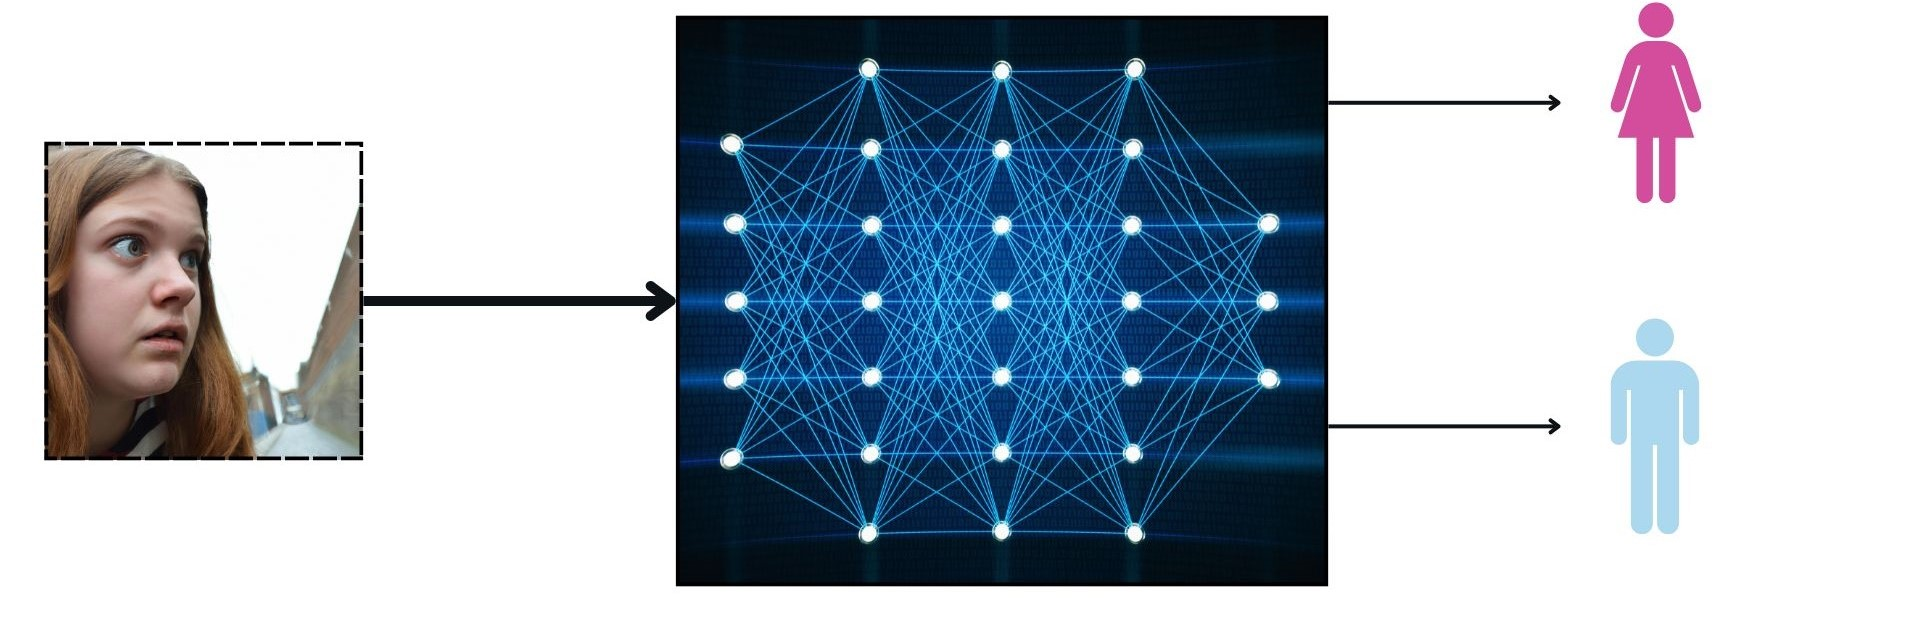
\includegraphics[width=0.85\textwidth]{imgs/CNN_eg.jpg}
\caption{Example Usage of Convolutional Neural Networks for Gender Classification }\label{fig:CNN_example}
\end{figure}

\noindent Before diving into the details of CNNs, let's start with the basics: What is an image to a computer, and what are computer vision tasks?

CNN (သို့မဟုတ်) Convolutional Neural Network သည် visual data / image များနှင့် သက်ဆိုင်သည့် လုပ်ငန်းများကို ဆောင်ရွက်နိုင်ရန်အတွက် ရည်ရွယ်တည်ဆောက်ထားသည့် deep learning architecture များ ဖြစ်သည်။ CNN ကို ဓါတ်ပုံ တစ်ခု ပေးလိုက်ပါက ပုံကို အမျိုးအစား ခွဲခြားပေးနိုင်ခြင်း ၊ ပုံတွင်ပါ၀င်သည့်အရာများကို အုပ်စုဖွဲ့ပေးနိုင်ခြင်း တို့ကို အလိုအလျောက်လုပ်ဆောင်ပေးနိုင်သည်။ Figure \ref{fig:CNN_example}  တွင် CNN ကို အသုံးပြု၍ ဓါတ်ပုံတစ်ပုံအား ကျား/မ ခွဲခြားခြင်းကို ပြသထားသည်။ Support Vector Machine (SVM), Logistic Regression စသည့် Classifier များနှင့် နှိုင်းယှဥ်လျှင် CNN သည် data pre-processing လုပ်ရသည့်အပိုင်းကို အများကြီးလျော့ချပေးနိုင်သည်။ 

\section{Understanding Images and Computer Vision Tasks}

\subsection{What is an image to a computer?}

To a computer, an image is represented as a grid of pixels. Each pixel is the smallest unit of the image and contains information about color and intensity. The structure of an image in a computer can be broken down into:
\begin{itemize}
  \item Grayscale Images: These images are represented by a 2D array where each element corresponds to a pixel. The value of each pixel ranges from 0 (black) to 255 (white). 
\begin{figure}[H]
    \centering
    \begin{minipage}{0.45\textwidth}
        \centering
        
\includegraphics[width=0.4\textwidth]{imgs/grayimg.png}                
    \end{minipage}\hfill
    \begin{minipage}{0.45\textwidth}
        \centering
        \[
        \begin{bmatrix}
            34  &  67  & 123 &  89 &  56 \\
            12  & 200 & 189 &  56 &  78 \\
            98  &  45 &  34 &  12 &  67 \\
            56  &  89 & 145 &  34 &  23 \\
            78  & 134 &  56 &  67 & 123 \\
        \end{bmatrix}
        \]
    \end{minipage}
    \caption{Example of a gray image and its representation in computer}
    \label{fig:gray_img}
\end{figure}
  \item Colored Images: These images are represented by three 2D arrays, each corresponding to one of the color channels: Red, Green, and Blue (RGB). Each pixel is thus represented by a triplet of values, such as (R, G, B), where each value ranges from 0 to 255. 
      \begin{figure}[h]%
        \centering
        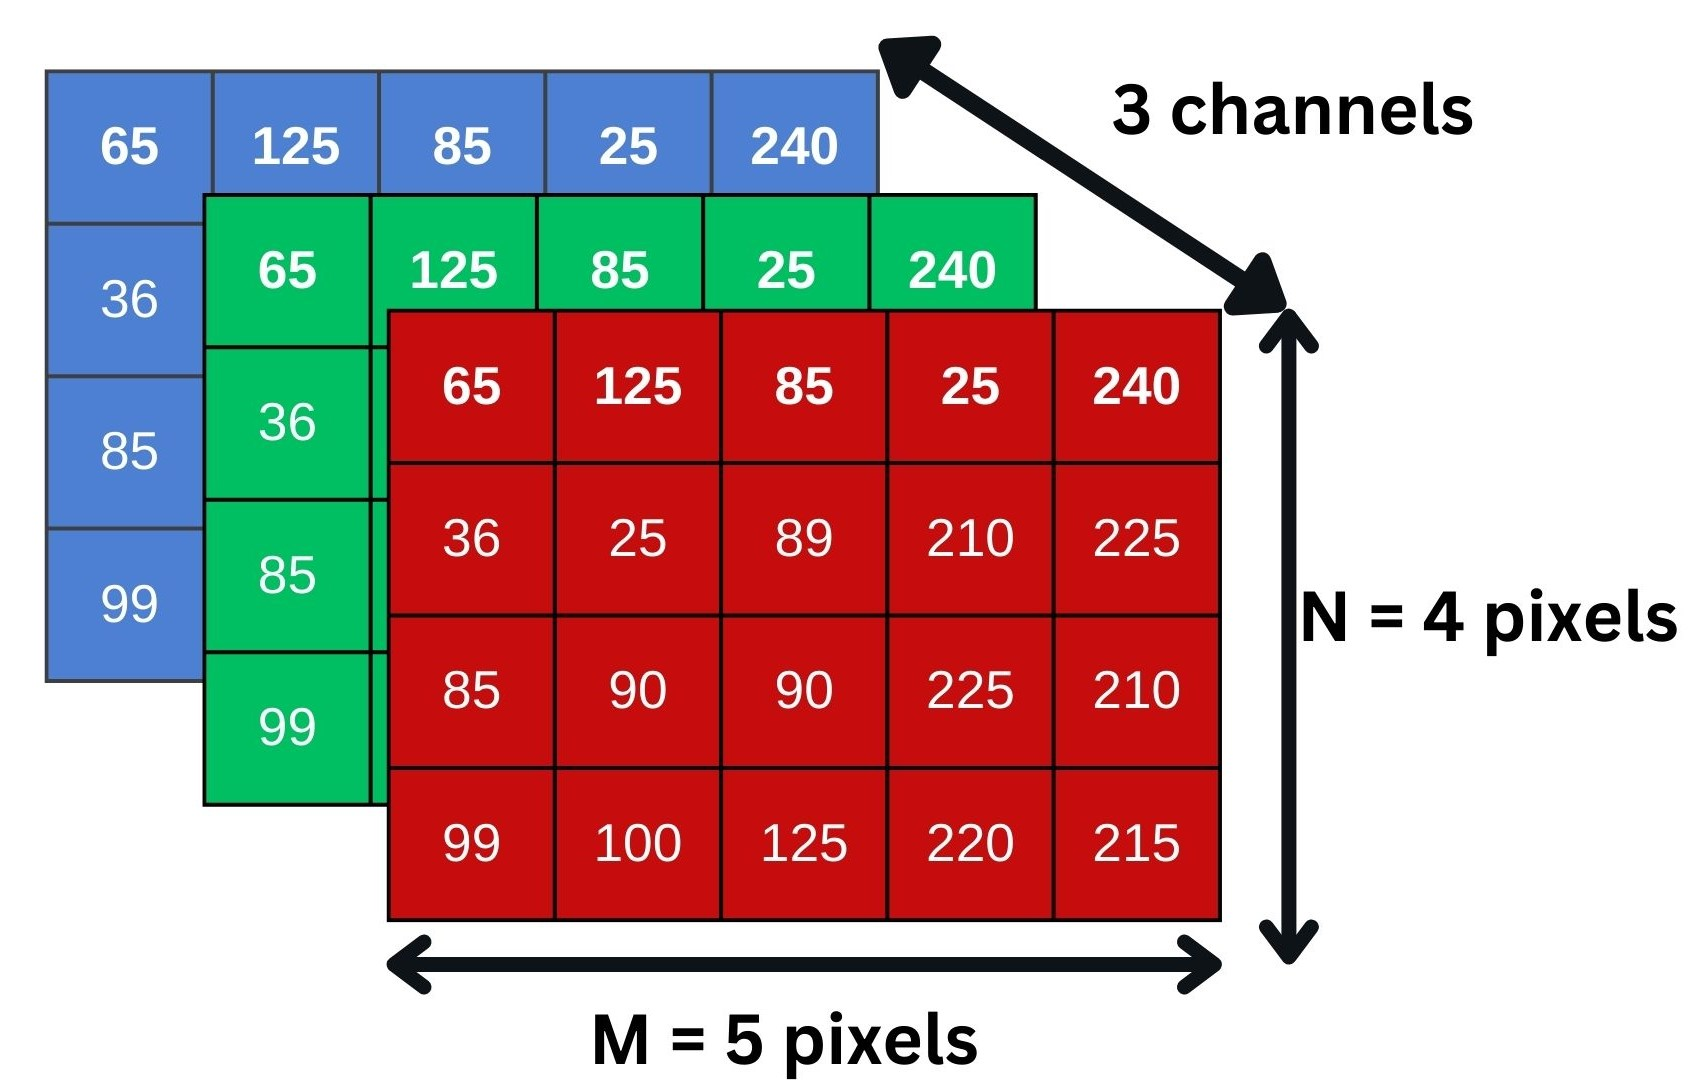
\includegraphics[width=0.75\textwidth]{imgs/colorImg.jpg}
        \caption{Representation of a color image with the resolution of 5 x 4. }\label{fig:colorImg}
        \end{figure}
\end{itemize}

Digital image တစ်ခုကို ကွန်ပြူတာတွင် ဖော်ပြရာ၌ ပုံ (\ref{fig:gray_img} - ဘယ်ဘက်) တွင် ဖော်ပြထားသော အဖြူအမည်း Image မျိုးဖြစ်ပါက pixel တစ်ခုချင်းစီ၏ intensity တန်ဖိုးများကို အသုံးပြုသည်။ pixel တစ်ခုချင်းစီ၏ intensity တန်ဖိုးသည် အဆိုပါ pixel နေရာ၏ အရောင်နှင့် အလင်းကို ဖော်ပြနိုင်သည်။ အဖြူရောင်ကို တန်ဖိုး အများဆုံး ဖြစ်သည့် -၂၅၅ ဖြင့်ဖော်ပြပြီး အနက်ရောက်ကို သုည အဖြစ် သိမ်းဆည်းသည်။ ဥပမာ -- ပုံ (\ref{fig:gray_img} - ဘယ်ဘက်) ၏ ဒုတိယ row ၏ အလယ် pixel နှစ်ခုသည် အခြား   pixel များထက် သိသိသာသာဖြစ်နေသည်ကို တွေ့နိုင်သည်။ ၄င်း  pixel နှစ်ခု၏ တန်ဖိုးကို  ပုံ(\ref{fig:gray_img} - ညာဘက်)ရှိ  matrix တွင်ကြည့်မယ်ဆိုပါက ၂၀၀ နှင့် ၁၈၉ ရှိသည်ကို တွေ့နိုင်သည်။ အခြား အမည်းရောင်ဘက်သို့ သွားသော pixel များ၏ တန်ဖိုးများမှာ နှစ်ဆယ်၊ သုံးဆယ် စသည့်ဖြင့် တစ်ရာ မကျော်သော ကိန်းဂဏန်းများဖြစ်သည်ကို တွေ့ရမည်။ 

Colored Image များကို ကွန်ပြူတာတွင် ဖော်ပြရာ၌ ပုံ (\ref{fig:colorImg}) တွင် ပြသထားသည့် အတိုင်း 3D-matrix ကို အသုံးပြုသည်။ Pixel တစ်ခု၏ color တန်ဖိုးကို Red, Green, Blue Channel များ အသုံးပြု၍ ဖော်ပြရာ အနီရောင် Pixel တစ်ခု၏ တန်ဖိုးမှာ [၂၅၅, ၀, ၀] ဖြစ်ပြီး အပြာရောင် Pixel တစ်ခု၏ တန်ဖိုးမှာ [၀, ၀, ၂၅၅] ဖြစ်မည်။ 

\subsection{Computer Vision Tasks}

Computer Vision is a field of artificial intelligence that enables computers to interpret and make decisions based on visual data from the world. Common tasks in computer vision include:

\begin{enumerate}
    \item \textbf{Image Classification}: Identifying the category or class of an object in an image. For example, recognizing whether an image contains a cat or a dog.
    \item \textbf{Object Detection}: Identifying and locating objects within an image, often by drawing bounding boxes around them. For instance, finding all the cars in a street image.
    \item \textbf{Segmentation}: Dividing an image into multiple segments or regions to simplify analysis. For example, segmenting a scene into trees, buildings and streets, etc. 
    \item \textbf{Biometric Recognition}: Identifying or verifying a person from an image by analyzing biometric features such as fingerprint and faces.
    \item \textbf{Pose Estimation}: Determining the pose of a human body or an object in an image, such as identifying the position and orientation of a person.
    \item \textbf{Optical Character Recognition (OCR)}: Converting different types of documents, such as scanned paper documents or images taken by a digital camera, into editable and searchable data.
    \item \textbf{Image Generation}: Creating new images from scratch or modifying existing images, such as in the case of Generative Adversarial Networks (GANs).
\end{enumerate}

Computer Vision သည် artificial intelligence (AI) လောက၏ အရေးကြီးသော အစိတ်အပိုင်း တစ်ခု ဖြစ်သည်။ ဓါတ်ပုံနှင့် ဗွီဒီယိုများကို ကွန်ပြူတာမှ လူများ နားလည်သကဲ့သို့ နားလည်နိုင်ရန် ထိုဓါတ်ပုံများကို ကြည့်၍ ဆုံးဖြတ်ချက်ချနိုင်ရန် သင်ပေးရသော ဘာသာရပ် တစ်ခုဖြစ်သည်။ Computer Vision ၏ လုပ်ငန်းအချို့မှာ -- 
\begin{itemize}
    \item \textbf{Image Classification}: Image တစ်ခုတွင် ပါ၀င်သည့် object ကို အမျိုးအစား ခွဲခြားပေးခြင်း။  ဥပမာ - လူတစ်ယောက်၏ ဓါတ်ပုံတစ်ပုံကို ပေးလိုက်ပါက Computer Vision Model မှ ကျား/မ ခွဲခြားပေးခြင်းသည် Image Classification / recognition ဖြစ်သည်။ 
    \item \textbf{Object Detection}: Image တစ်ခုတွင် ပါ၀င်သည့် object ကို ရှာဖွေပေးခြင်း။ ဥပမာ -- လမ်းမပေါ်ရှိ ကားများကို detect လုပ်ခြင်း။ 
    \item \textbf{Segmentation}: Image တစ်ခုကို မျိုးတူရာ အုပ်စု ခွဲခြားပေးခြင်း။ ဥပမာ -- Google Map မှ မြင်ရသော ပုံကို လမ်းများ၊ ကားများ၊ သစ်ပင်များ စသည်ဖြင့် တူရာ ခွဲခြားပေးခြင်း။ 
    \item \textbf{Biometric Recognition}:  လက်ဗွေရာ၊ မျက်နှာ စသည့် Biometric features များကို အသုံးပြု၍ လူတစ်ယောက်၏ identity ကို စစ်ဆေးခြင်း။ 
    \item \textbf{Pose Estimation}: လူတစ်ယောက်၏ Pose ကို ခန့်မှန်းခြင်း။ ဥပမာ -- သက်ကြီးရွယ်အိုများ လဲကျသည့် Pose ကို ခန့်မှန်းခြင်း။ 
    \item \textbf{Optical Character Recognition (OCR)}: Scanned ဖတ်ပြီး ရလာသည့် စာသားများကို Recognize လုပ်ပေးခြင်း။ 
    \item \textbf{Image Generation}: စာသား၊  အသံ (သို့မဟုတ်) ပုံရိပ်ဟောင်းများကို အသုံးပြု၍ ပုံရိပ်အသစ်များ တီထွင်ဖန်တီးခြင်း ။ 
    \end{itemize}

\newpage
\section{Architecture of Convolutional Neural Network}\label{CNN_architecture}

The architecture of a Convolutional Neural Network (CNN) encompasses several key components, each playing a crucial role in the network's ability to learn and make predictions. An example of CNN is given in Figure \ref{fig:CNN}. The Convolutional Layer and the Pooling Layer, together form the i-th layer of a Convolutional Neural Network. The convolution layers focus on learning feature representations, and the pooling layers help in summarizing these features. Depending on the complexities in the images, the number of such layers may be increased for capturing low-level details even further, but at the cost of more computational power. 

\vspace{0.5em}
\begin{figure}[h]%
\centering
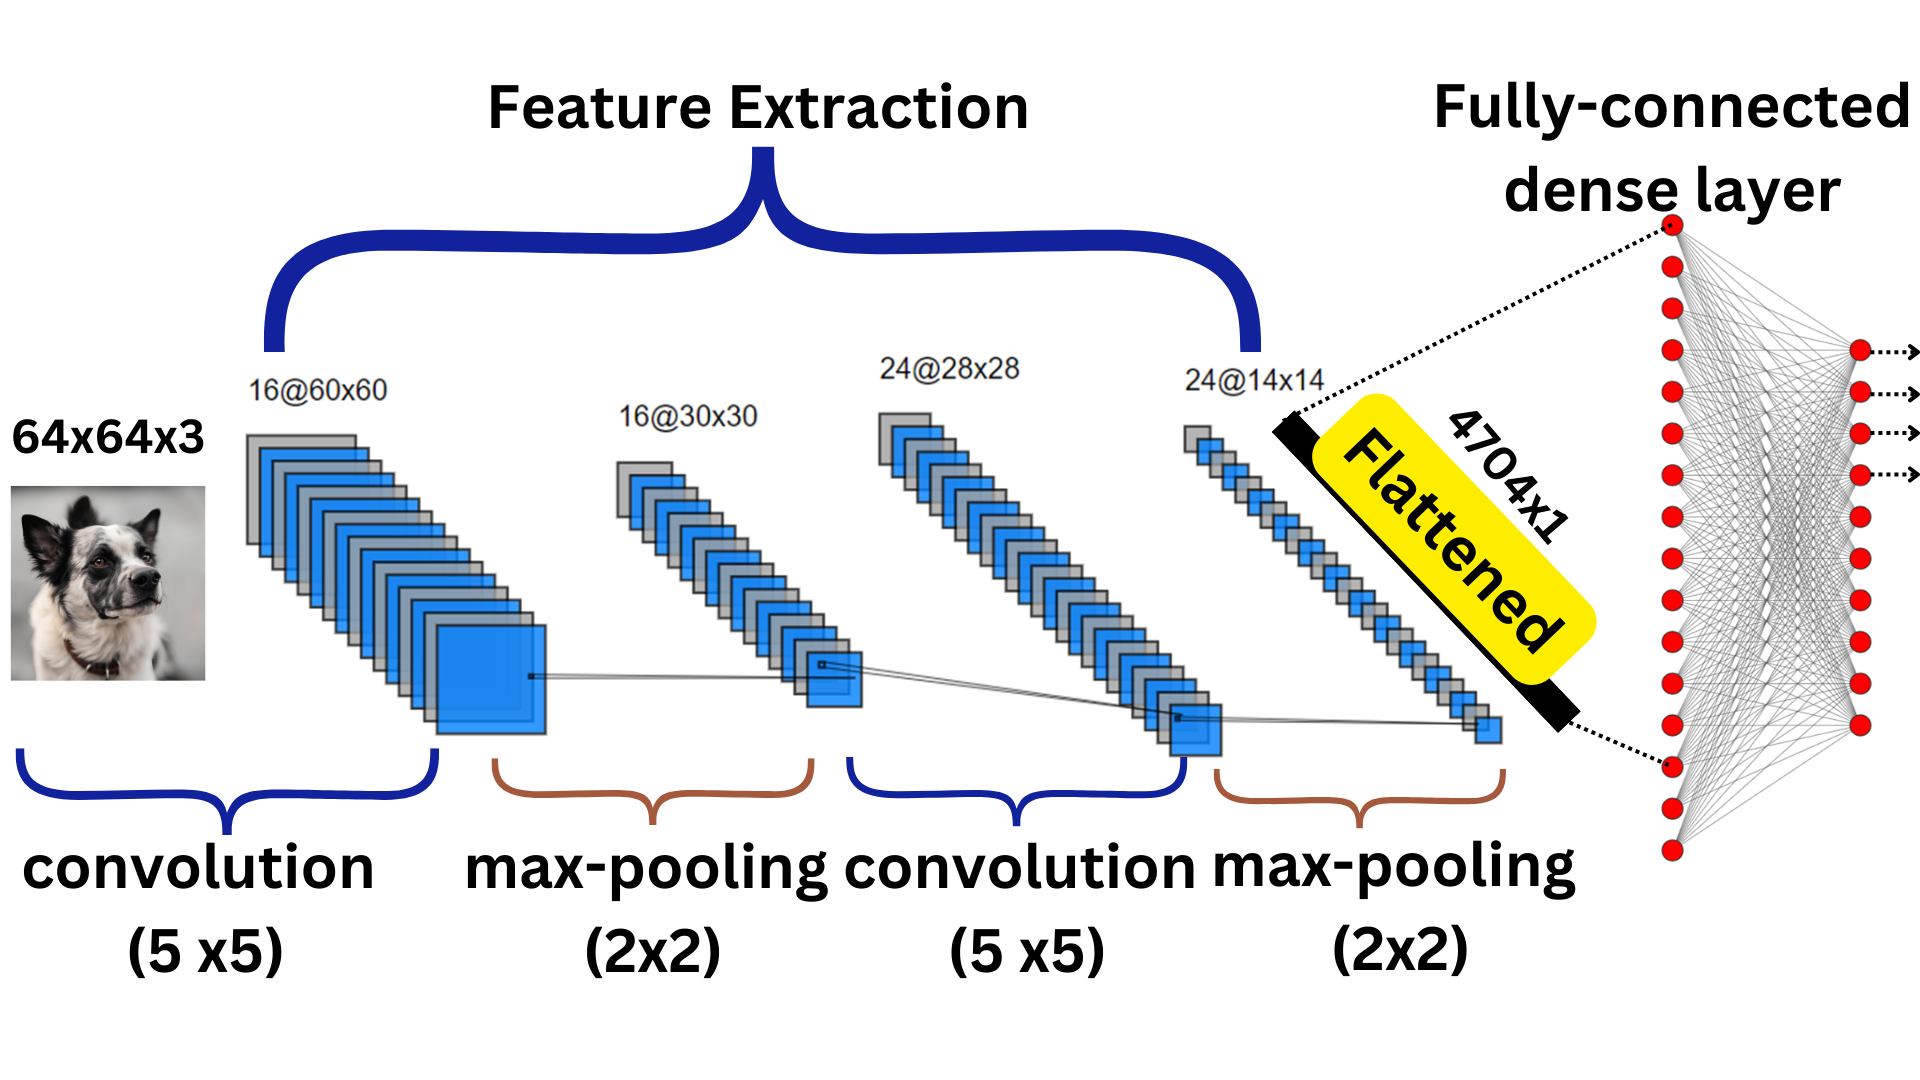
\includegraphics[width=0.8\textwidth]{imgs/cnn_own.png}
\caption{Example of Convolutional Neural Networks.}\label{fig:CNN}
\end{figure}

Integrating the extracted features from convolutional and pooling layers, the fully connected layers establish connections between every neuron in one layer with every neuron in the subsequent layer, similar to traditional neural networks. These layers captures global patterns and relationships within the data, ultimately forming a high-level representation suitable for classification or regression tasks. Notably, the final fully connected layer often serves as the output layer, generating predictions based on the learned features.

CNN  တစ်ခု၏  architecture တွင် အခြေခံအားဖြင့် convolutional, pooling, နှင့် fully connected (dense) layer တို့ ပါ၀င်သည်။ Figure \ref{fig:CNN} တွင် ပြသထားသည့်အတိုင်း Convolution နှင့် Pooling Layer -- ၂ ခု ကို တစ်စုံ အဖြစ် စဥ်းစားနိုင်သည်။ Convolution layer သည် feature များကို ရှာဖွေရန် အဓိက တာ၀န်ယူပြီး Pooling Layer သည် အရေးကြီး သော feature များကို ထုတ်ယူရန် တာ၀န်ယူသည်။ CNN  တစ်ခုတွင် Convolution နှင့် Pooling Layer များစွာ ပါ၀င်နိုင်သည်။  

Fully connected layer သည် ဤ Layer များမှ ရရှိလာသော feature များကို ခြုံငုံချိတ်ဆက်ပေးသည်။           

\subsection{Convolutional Layer}\label{convLayer}

The convolutional layer is a fundamental building block of a CNN. It applies learnable filters, also known as kernels, to the input data using the convolution operation. A kernel (or filter) in the context of convolution is a small matrix that moves over the input data and performs element-wise multiplications followed by a summation to produce a single output value. This process is repeated across the entire input, producing a feature map (or activation map).

\noindent Consider a simple 5x5 grayscale image and a 3x3 kernel given below:
\[
\begin{array}{cc}
\text{Grayscale Image:} & \text{Kernel Matrix:} \\
\begin{bmatrix}
    34  &  67  & 123 &  89 &  56 \\
    12  & 200 & 189 &  56 &  78 \\
    98  &  45 &  34 &  12 &  67 \\
    56  &  89 & 145 &  34 &  23 \\
    78  & 134 &  56 &  67 & 123 \\
\end{bmatrix} & 
\begin{bmatrix}
    1 & 0 & -1 \\
    1 & 0 & -1 \\
    1 & 0 & -1 \\
\end{bmatrix}
\end{array}
\]

The process of convolution involves moving the kernel across the input image and performing element-wise multiplication followed by summation at each location. For instance, at the very first location, the kernel will be multiplied with the pixel intensities highlighted in yellow. The element-wise multiplication and sum will produce the convolution result of 
\begin{equation}\label{eqn:convEg}
(34+12+98)+(0+0+0)-(123+189+34) =-202
\end{equation}

The result of this calculation is the value for the first position of the output matrix, highlighted in the Feature Map (right). Then, the kernel is moved to the next position (in this example, moved by Stride = 1 pixel) and the process is repeated for the entire input image, leading to the resulting matrix:

\[
\begin{array}{cc}
\text{Grayscale Image:} & \text{Convoluted Results (Feature Map)} \\
\begin{bmatrix}
    \colorbox{yellow}{$34$}  &  \colorbox{yellow}{$67$}  & \colorbox{yellow}{$123$} &  89 &  56 \\
    \colorbox{yellow}{$12$}  & \colorbox{yellow}{$200$} & \colorbox{yellow}{$189$} &  56 &  78 \\
    \colorbox{yellow}{$98$}  &  \colorbox{yellow}{$45$} &  \colorbox{yellow}{$34$} &  12 &  67 \\
    56  &  89 & 145 &  34 &  23 \\
    78  & 134 &  56 &  67 & 123 \\
\end{bmatrix} & 
\begin{bmatrix}
    \colorbox{yellow}{$-202$} & 155 & 145 \\
    -202 & 232 & 200 \\
    -3 & 155 & 22 \\
\end{bmatrix}
\end{array}
\]

The size of the feature map (or output) generated by a convolutional layer in a Convolutional Neural Network (CNN) is generally smaller than the input size. This reduction in size depends on several factors, including the kernel size, stride length, and whether padding is applied. In the above example, for a 3x3 kernel with a stride length of 1 and no padding, the feature map produced will be smaller, typically by 2 pixels in each dimension. So, if the input is, for instance, a 64x64 image, the resulting feature map will be 62x62.

The kernel used in the convolution operation determines the types of features detected. The provided kernel function in the above example detects the vertical edges in the image, meaning the pixels where there are vertical edges will have high intensity values in the convolved image. In traditional image processing, kernels are defined by the programmer, and some commonly used kernels include:
\begin{enumerate}
\item \textbf{Laplacian Kernel}: This kernel is employed for edge detection and highlighting areas of rapid intensity change.
\item \textbf{Edge Detector (Sobel Filter)}: It's utilized for detecting edges in specific directions.
\item \textbf{Average Kernel (Box Filter)}: This kernel is applied for blurring or smoothing the image.
\end{enumerate}

However, in Convolutional Neural Networks (CNNs), each convolutional layer employs multiple filters to create multiple feature maps. These filters are initialized randomly and then adjusted during training to minimize the loss function. This adjustment process allows the filters to learn to detect various features automatically, such as edges, patterns, and complex structures, making CNNs highly effective for tasks like image classification and object detection.

Convolutional layer သည် CNN  architecture ၏ အရေးကြီးသော အစိတ်အပိုင်း တစ်ခု ဖြစ်သည်။ ဤ layer တွင် filter (kernel) များကို အသုံးပြု၍ image (input data) တွင် ပါ၀င်သည့် အရေးကြီးသော feature များကို ရှာဖွေသည်။ ဤနေရာတွင် kernel ဆိုသည်မှာ k x k matrix တစ်ခုသာ ဖြစ်သည်။ အထက်တွင် 3 x 3 kernel နမူနာ တစ်ခုကို ဖော်ပြထားသည်။ Convolution ပြုလုပ်သည် ဆိုခြင်းမှာ အဆိုပါ kernel ကို image တလျောက် နေရာရွေ့၍  kernel နှင့် input data ကို မြှောက်၍ ပေါင်းလဒ်ကို ရှာဖွေခြင်း ဖြစ်သည်။ 

အထက်ပါ ဥပမာ ကို ကြည့်မည်ဆိုပါက feature map ၏ ပထမဆုံး တန်ဖိုးသည် image ၏ ပထမဆုံး pixel ကိုးခုနှင့် kernel ၏ တန်ဖိုးများကို မြှောက်၍ စုစုပေါင်းတန်ဖိုး  ($(34+12+98)+(0+0+0)-(123+189+34) =-202$) ကို ရှာဖွေခြင်း ဖြစ်သည်။ ယခု ဥပမာ တွင် အသုံးပြုထားသည့် kernel သည် ဒေါင်လိုက် Line များကို ရှာဖွေရာတွင် အသုံးပြုနိုင်သည်။ image processing များ ပြုလုပ်ရာတွင် ဒေါင်လိုက်၊ အလျားလိုက်နဲ့ ဒေါင့်ဖြတ်ဖြစ်နေသာ လိုင်းများကို ရှာဖွေပေးသည့် အထက်ပါ Edge Detector များအပြင် ပျမ်းမျှ တန်ဖိုးကို ရှာဖွေပေးသော Average Kernel များ ၊ ရုတ်တရက် intensity တန်ဖိုးပြောင်းသွားသည့် Edge ကို ရှာဖွေပေးသည့် Laplacian Kernel များကိုလည်း အသုံးပြုကြသည်။ 

သို့သော် CNN တွင်မူ convolutional layer တစ်ခုတွင် filter တစ်ခုမက အသုံးပြုပြီး filter ကို ကြိုတင်သတ်မှတ်ထားရန် မလိုအပ်ပါ။ Training ပြုလုပ်ရာတွင် loss (input output ကြား ကွာခြားချက်) အနည်းဆုံး ဖြစ်စေမည့် filter ကို Optimization algorithm များ အသုံးပြု၍ ရှာဖွေသည်။ ထိုသို့ရှာဖွေဖြင်းဖြင့် image များကို အမျိုးအစားခွဲခြားခြင်း ၊ object ကို ရှာဖွေခြင်း စသည့် task များအတွက် အသုံး၀င်မည့် feature များကို ရရှိပြီး CNN ၏ Performance ကို ပိုမို ကောင်းမွန်စေသည်။ 


\subsection{Pooling Layer}\label{poolLayer}
The pooling layer serves to decrease the spatial dimensions of feature maps while retaining crucial information. Common pooling operations include max pooling and average pooling, which aid in achieving translation invariance and computational efficiency. There are two primary types of pooling: Max Pooling and Average Pooling.

\vspace{0.5em}
\begin{figure}[h]%
\centering
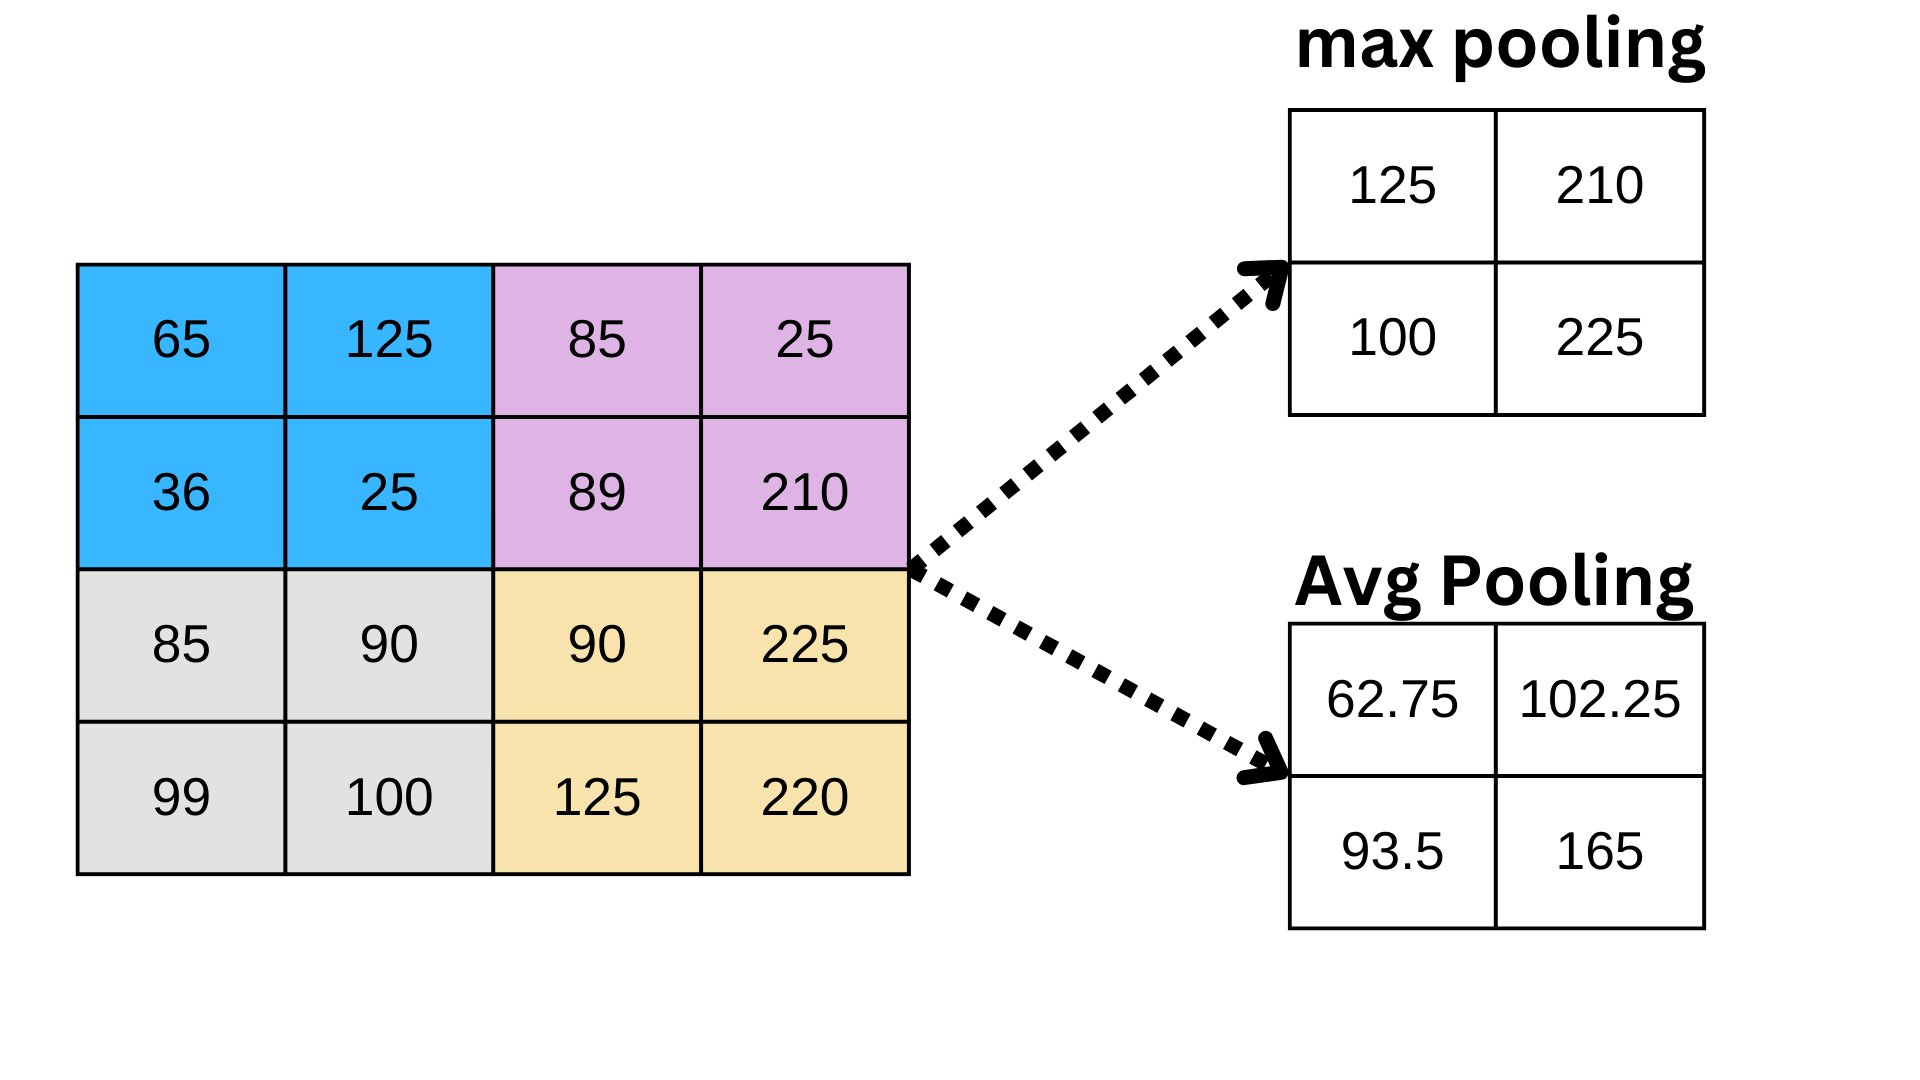
\includegraphics[width=0.75\textwidth]{imgs/cnn_pool.png}
\caption{Example of max-pooling and average pooling.}\label{fig:CNNPooling}
\end{figure}

Max Pooling selects the maximum value from the section of the image covered by the kernel, whereas Average Pooling computes the average of all the values within the kernel's coverage area. In Figure \ref{fig:CNNPooling}, the operation of both max pooling and average pooling on a 4x4 convoluted image is illustrated.

By utilizing a 2x2 kernel in the pooling layer, the size of the input data is halved. For example, if the input (convoluted map) is a 62x62 image, the resulting matrix will be reduced to 31x31.


\subsection{Fully Connected Layer}\label{FCLayer}
Once the convolutional and pooling layers have extracted important features, the model proceeds to a fully connected layer. Here, the final output from these layers is flattened and fed into a traditional feed-forward neural network for classification or regression tasks.

The fully connected layer learns non-linear combinations of the high-level features represented by the output of the convolutional and pooling layers. Through forward and backpropagation, the feed-forward neural network adjusts its parameters to understand the complex relationships within the data. Over multiple epochs, the model distinguishes between dominant and subtle features in the images, utilizing an appropriate activation function to produce the output.

The choice of activation function in the output layer depends on the task at hand. For binary classification, a sigmoid activation function is often chosen, while for multi-class classification, a softmax activation function is commonly used. In regression tasks, the output layer typically comprises a single neuron with a linear activation function, generating a continuous output value.

Fully Connected Layer သည် ပြီးခဲ့သည့် အခန်းတွင် ရှင်းပြခဲ့သည့် Feed-forward neural network ၏ hidden layer (သို့မဟုတ်) output layer များနှင့် သဘောတရားအတူတူပင် ဖြစ်သည်။ Convolution နှင့် Pooling Layer များမှ အရေးကြီးသည့် features များကို သင်ယူပြီးနောက် ဤ Layer များ၏ final output မှာ feature vector တစ်ခု ဖြစ်သည်။  အဆိုပါ feature vector သည်  Feed-forward neural network (MLP) ၏ input vector ဖြစ်မည်။ ထို့နောက် MLP မှ forward နှင့် backward propagation ကို ကြိမ်ဖန်များစွာ ပြုလုပ်ပြီး model အတွက် လိုအပ်သည့် parameters များကို Feature (training set) မှ ရှာဖွေမည် ဖြစ်သည်။ 

Feed-forward neural network တွင် Fully Connected hidden layer တစ်ခု (သို့မဟုတ်)နှစ်ခု နှင့် output layer တစ်ခုတို့ ပါ၀င်သည်။ နောက်ဆုံး Fully Connected output layer တွင် အသုံးပြုမည့် activation function သည် လုပ်ဆောင်မည့် လုပ်ငန်းပေါ်တွင် မူတည်၍ ရွေးချယ်ရမည်။ အမျိုးအစား ၂ ခု ကိုသာ ခွဲခြားပေးသော Binary Classification ပုစ္ဆာများတွင် sigmoid activation function ကို အသုံးပြုပြီး multi-class classification တွင်မူ softmax activation function ကို အသုံးပြုကြသည်။ Output Layer တွင် ပါ၀င်ရမည့် unit (neuro) မှာ ခွဲခြားပေးရမည့် Output အရေအတွက်ပေါ်တွင် မူတည်သည်။ ဥပမာ -- ခွေး(သို့မဟုတ်) ကြောင် ဟု ခွဲခြားပေးမည့် Classifier ၏ Output Layer ရှိ unit (neuro) အရည်အတွက်မှာ ၂ ဖြစ်ပြီး လက်ရေးဖြင့်ရေးထားသော number များကို ခန့်မှန်းမည့် Classifier အတွက်မူ unit (neuro) အရည်အတွက် တစ်ဆယ် (သုညမှ ၉ အထိ) ဖြစ်ရမည်။ Regression အတွက်မူ unit (neuro) တစ်ခုသာ ပါ၀င်ပြီး linear activation function ကို အသုံးပြုသည်။ 

\setcounter{stepcounter}{0}
\subsection{Building a CNN Architecture}
This section gives an example of how to build a Convolutional Neural Network (CNN) architecture using the `keras` library in Python. The model is structured as a sequential model, integrating multiple convolutional layers, max-pooling layers, a flattening layer, and fully connected layers, as demonstrated in Figure \ref{fig:CNNArch}.

ဤအခန်းတွင် Convolutional Neural Network (CNN) architecture တစ်ခုကို `keras` library အသုံးပြုပြီး တည်ဆောက်ပြထားခြင်း ဖြစ်ပါသည်။ Python ကုဒ်များဖြစ်သည့်အတွက် မြန်မာဘာသာ ပြန်ဆိုခြင်း မပြုထားပါ။ စာဖတ်သူများအနေဖြင့် ပေးထားသည့် GitHub Repo ကို Fork လုပ်၍ Python ကုဒ်များကို တစ်ကြောင်းချင်း run ကြည့်ရန် အကြံပြုပါသည်။ ဤ architecture တွင် convolutional layer သုံးစုံ၊ flattening layer တစ်ခုနှင့် fully connected layer နှစ်ခုတို့ ပါ၀င်ရာ layer တစ်ခုချင်းစီကို architecture ထဲသို့ မည်သို့ ထည့်ရမည်ကို အဆင့် (၅) ဆင့်ဖြင့် ရှင်းလင်းပြထားပါသည်။ ပါ၀င်သည့် layer တစ်ခုချင်းစီအတွက် လိုအပ်သည့် parameter အရည်အတွက်များကို နောက်အခန်းတွင် အသေးစိပ် ရှင်းပြသွားမည်။ 

\vspace{0.5em}
\begin{figure}[h]%
\centering
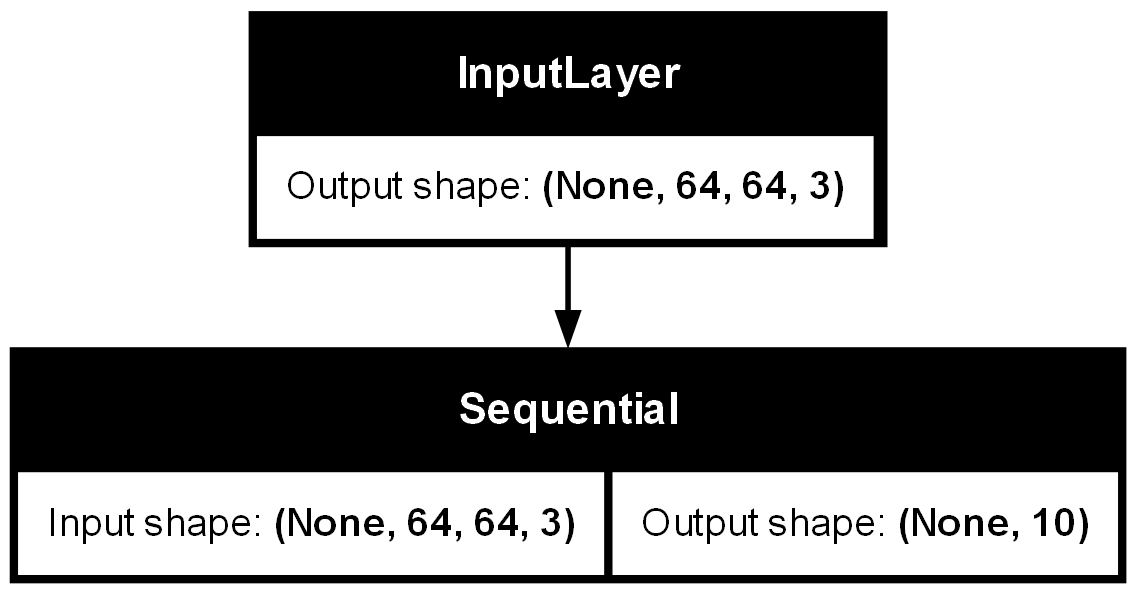
\includegraphics[width=0.55\textwidth]{imgs/cnn_model_seq.png}
\caption{Example of CNN Model Architecture}\label{fig:CNNArch}
\end{figure}

\begin{step}
First, an input layer is defined to specify the shape of the input data. In general, the shape of the input data is the size of the image. 
\begin{verbatim}
inputs = Input(shape=input_shape)
\end{verbatim}
\end{step}

\begin{step}
A Sequential model is then, constructed to define the architecture of the CNN.
\begin{verbatim}
model = Sequential()
\end{verbatim}
\end{step}
\begin{step}
In this step, three convolutional layers, each comprising a convolutional layer followed by a max-pooling layer, are added to the sequential model defined in Step 2.
\paragraph*{Convolutional Layer 1}
\begin{itemize}
    \item \texttt{Conv2D}: 32 filters, kernel size of 5x5, activation function \texttt{relu}.
    \item \texttt{MaxPooling2D}: Pool size of 2x2.
\end{itemize}
\begin{verbatim}
model.add(Conv2D(32, (5, 5), activation='relu'))
model.add(MaxPooling2D((2, 2)))
\end{verbatim}

\paragraph*{Convolutional Layer 2}
\begin{itemize}
    \item \texttt{Conv2D}: 64 filters, kernel size of 5x5, activation function \texttt{relu}.
    \item \texttt{MaxPooling2D}: Pool size of 2x2.
\end{itemize}
\begin{verbatim}
model.add(Conv2D(64, (5, 5), activation='relu'))
model.add(MaxPooling2D((2, 2)))
\end{verbatim}

\paragraph*{Convolutional Layer 3}
\begin{itemize}
    \item \texttt{Conv2D}: 128 filters, kernel size of 5x5, activation function \texttt{relu}.
    \item \texttt{MaxPooling2D}: Pool size of 2x2.
\end{itemize}
\begin{verbatim}
model.add(Conv2D(64, (5, 5), activation='relu'))
model.add(MaxPooling2D((2, 2)))
\end{verbatim}
\end{step}

\begin{step}
In Step 4, the output from the convolutional layers undergoes flattening, transforming the 2D matrix data into a 1D vector. This flattened representation is then fed into two fully connected layers. Finally, the last layer serves as the output layer, containing 10 labels.

\paragraph*{Flattening Layer} 
\begin{verbatim}
model.add(Flatten())
\end{verbatim}

\paragraph*{Fully Connected Layer}
\begin{itemize}
    \item \texttt{Dense}: 512 units, activation function \texttt{relu}.
    \item \texttt{Output layer}: 10 units (assuming 10 classes for classification), activation function \texttt{softmax}.
\end{itemize}
\begin{verbatim}
model.add(Dense(512, activation='relu'))
model.add(Dense(10, activation='softmax'))
\end{verbatim}
\end{step}

\begin{step}
Finally, the model is built by specifying the inputs and outputs.
\begin{verbatim}
model = Model(inputs=inputs, outputs=model(inputs))
\end{verbatim}
\end{step}

\subsection{Parameter Analysis}
The total number of trainable parameters in a CNN model significantly impacts its capacity and performance. These parameters are influenced by factors such as the size of convolutional filters, the number of filters in each layer, and the dimensions of fully connected layers.

\begin{table}[htbp]
    \centering    
    \caption{Summary of CNN Model Architecture}
    \label{tab:cnnR}
    \begin{tabular}{|l|l|l|}
    \hline
    \textbf{Layer (type)}             & \textbf{Output Shape}   & \textbf{Param \#} \\
    \hline
    input\_layer\_2 (InputLayer)      & (None, 64, 64, 3)       & 0                 \\
    \hline
    conv2d\_3 (Conv2D)                & (None, 60, 60, 32)      & 2,432             \\
    \hline
    max\_pooling2d\_3 (MaxPooling2D)  & (None, 30, 30, 32)      & 0                 \\
    \hline
    conv2d\_4 (Conv2D)                & (None, 26, 26, 64)      & 51,264            \\
    \hline
    max\_pooling2d\_4 (MaxPooling2D)  & (None, 13, 13, 64)      & 0                 \\
    \hline
    conv2d\_5 (Conv2D)                & (None, 9, 9, 128)       & 204,928           \\
    \hline
    max\_pooling2d\_5 (MaxPooling2D)  & (None, 4, 4, 128)       & 0                 \\
    \hline
    flatten\_1 (Flatten)              & (None, 2048)            & 0                 \\
    \hline
    dense\_2 (Dense)                  & (None, 512)             & 1,049,088         \\
    \hline
    dense\_3 (Dense)                  & (None, 10)              & 5,130             \\
    \hline
    \end{tabular}
\end{table}

Table \ref{tab:cnnR} provides a breakdown of the parameters for each layer of the CNN model outlined above. The input layer simply defines the shape of the input image and does not have any trainable parameters. Hence, the number of parameters for the input layer is zero. 

The convolutional layers are where CNN learns the features and these layers contribute significantly to the total parameter count. Typically, the number of parameters in a convolutional layer is calculated by multiplying the filter width $m$, by the filter height $n$, by the depth $d$ of the input volume, and the number of filters $k$ in the current layer, and then adding bias terms for each filter. For example, in Convolutional Layer 1, the number of parameters is calculated as $(5 \times 5 \times 3 \times 32) + 32 = 2,432$.

The max-pooling layer does not have any parameters, as it simply selects the maximum value from the input regions and does not involve any learning process. In contrast, the fully connected layers have the highest number of parameters because every neuron in the previous layer is connected to every neuron in the current layer. Hence, the number of parameters is the product of the number of neurons in the current layer $c$ and the number of neurons in the previous layer $p$, plus the bias terms. For example, the number of parameters for the first fully connected layer is calculated as follows: $((c * p)+1*c = 512*2048 + 512 = 1,049,088)$.

The number of parameters in the CNN model directly affects the computational resources required for training and inference. Larger models with more parameters demand higher computational resources and longer training times, making scalability an important consideration in model development and deployment.

CNN model တစ်ခု၏ performance သည် အဆိုပါ model တွင် ပါ၀င်သည့် parameter အရေအတွက် ပေါ်တွင် မူတည်သည်။ အထက်ပါ ဇယားတွင် CNN model တစ်ခု၏ layer အသီးသီးတွင် ပါ၀င်သည့် parameter အရေအတွက်ကို ဖော်ပြထားပြီး တွက်ချက်ပုံ အဆင့်ဆင့်ကို ရှင်းပြသွားမည်။ ဤသင်ခန်းစာတွင် နမူနာပြထားသည့် Model တွင် Input image သည် color image တစ်ခုဖြစ်ပြီး ၄င်း၏ အရွယ်အစားမှာ  $(64 \times  64)$ ဖြစ်သည်။ input layer တွင် parameter ကို တွက်ချက်ရန် မလိုအပ်ပါ။  

Convolutional layer များတွင် လိုအပ်သည့် parameter အရေအတွက်သည် convolutional filter ၏ အရွယ်အစား၊ filter အရေအတွက်များ အပေါ်တွင် မူတည်သည်။ ဥပမာ ဒုတိယ layer တွင်  $(5 \times 5 )$ convolutional filter ကို အသုံးပြုထားပြီး filter အရေအတွက်မှာ သုံးဆယ့်နှစ်ခု ဖြစ်သည်။ထို့ပြင် မူလ Input image တွင် channel သုံးခုပါ၀င်ရာ ဤ convolutional layer တွင် တွက်ချက်ရမည့် parameter အရေအတွက်မှာ $(5 \times 5 \times 3 \times 32) + 32 = 2,432$, နှစ်ထောင့် လေးရာ သုံးဆယ့်နှစ်ခု ဖြစ်သည်။ ထည့်ပေါင်းထားသည့် ၃၂ မှာ filter တစ်ခုချင်းစီအတွက် bias term တစ်ခု စီ ထည့်ပေါင်းထားခြင်း ဖြစ်သည်။ 

max-pooling layer သည် filter အတွင်းရှိ အကြီးဆုံး တန်ဖိုးကို ဆွဲထုတ်ခြင်းသာ ဖြစ်ရာ parameter ကို တွက်ချက်ရန် မလိုအပ်ပါ။  များသောအားဖြင့် CNN model  တွင် parameter အများဆုံးသော layer မှာ fully connected layer များဖြစ်သည်။ fully connected ဟုဆိုသည့်အတိုင်း ပြီးခဲ့သည့် layer ၏ neuron တစ်ခုတိုင်းသည် ယခု layer ၏ neuron တိုင်းနှင့်ချိတ်ဆက်ထားသည် ဖြစ်ရာ parameter အရေအတွက်မှာ  layer နှစ်ခု၏ neuron  အရည်အတွက် မြှောက်ခြင်း ဖြစ်သည်။ ဥပမာ - ယခု နမူနာပြထားသည့် Model ၏ ပထမ fully connected layer တွင် neuron အရေအတွက်မှာ  ငါးရာတစ်ဆယ့်နှစ်ခု ရှိပြီး flattened Layer တွင် ရှိသည့် neuron အရေအတွက်မှာ  နှစ်ထောင့်လေးဆယ့်ရှစ်ခုဖြစ်သည်။ သို့ဖြစ်ရာ ပထမ fully connected layer အတွက်  လိုအပ်သည့် parameter အရေအတွက်မှာ တစ်သန်း လေးသောင်း ကိုးထောင် ရှစ်ဆယ့် ရှစ်ခု $((c * p)+1*c = 512*2048 + 512 = 1,049,088)$ ဖြစ်သည်။ 

CNN model တစ်ခုတွင် တွက်ချက်ရန် လိုအပ်သည့် parameter များလာသည်နှင့် အမျှ model ကို Training ပြုလုပ်ရန် အသုံးပြရသည့် ကြာချိန် ပိုကြာမြင့်လာပြီး computational resource များလည်း ပိုမို လိုအပ်လာသည်။ 

\newpage
\section{Various architectures of CNNs}\label{sec:vCNN}

There are numerous architectures of Convolutional Neural Networks (CNNs), each designed to address different challenges and tasks in the field of computer vision. They are typically different based on the number of layers and activation functions used. In this section, a few backbone CNN architectures are discussed. 

Convolutional Neural Network architecture တွင် အသုံးပြုသည့် activation function အမျိုးအစား၊ convolutional နှင့် fully connected layer အရည်အတွက် ပေါ်တွင် မူတည်၍ Convolutional Neural Network အမျိုးမျိုး ရှိသည်။ ဤအခန်းတွင် လူသုံးများသည့် CNN architecture အချို့ကို ဆွေးနွေးသွားမည်။ 

\subsection{AlexNet}

AlexNet \cite{AlexNet2012} is a convolutional neural network (CNN) architecture that was developed by Alex Krizhevsky, Ilya Sutskever, and Geoffrey Hinton. It won the ImageNet Large Scale Visual Recognition Challenge (ILSVRC) in 2012. The AlexNet architecture consists of eight layers: five convolutional layers, some of which are followed by max-pooling layers, two fully connected hidden layers, and one fully connected output layer.

\vspace{0.5em}
\begin{figure}[h]%
\centering 
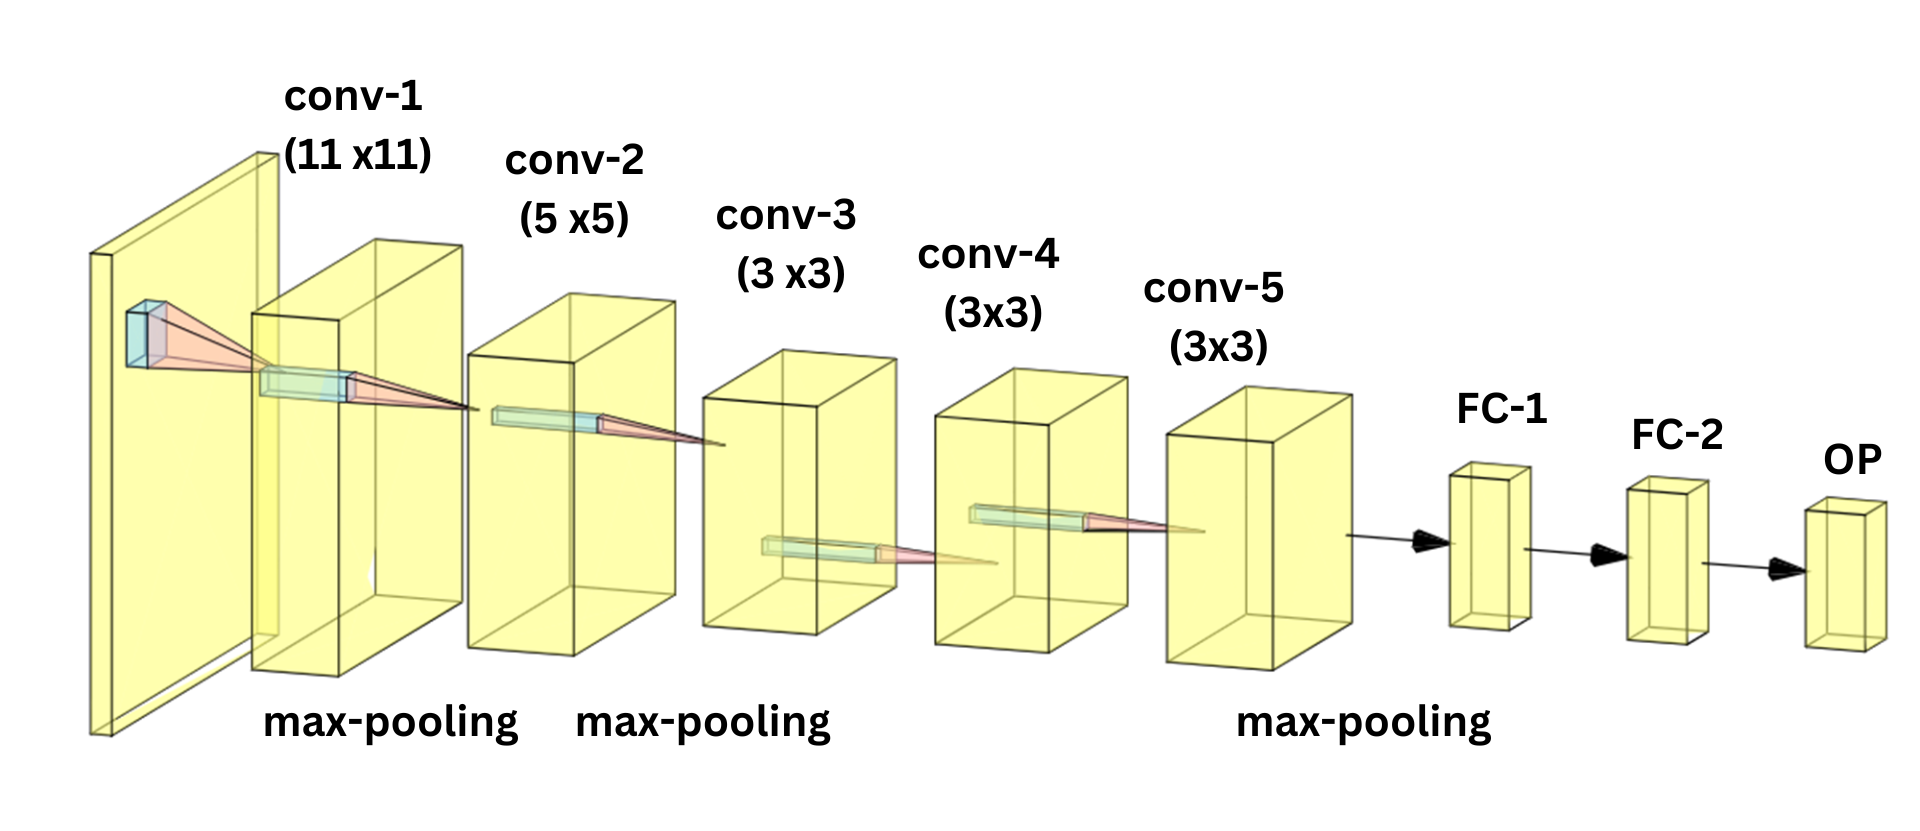
\includegraphics[width=0.75\textwidth]{imgs/alexnet.png}
\caption{AlexNet Architecture. Image created by\cite{web:NNSVG}}\label{fig:alexnet}
\end{figure}

AlexNet သည် Alex Krizhevsky, Ilya Sutskever, နှင့် Geoffrey Hinton တို့ တီထွင်ခဲ့သော convolutional neural network architecture ဖြစ်သည်။ ၂၀၁၂ ခုနှစ် ILSVRC ပြိုင်ပွဲတွင် ဆုရရှိခဲ့သည်။ AlexNet architecture တွင် convolutional layer ၅ ခု ၊ fully connected hidden layer - နှစ်ခုနှင့် output layer - တစ်ခု တို့ပါ၀င်သည်။ အချို့ convolutional layer များတွင် တွဲဖက်ဖြစ်သော max-pooling layer ပါ၀င်သည်။ 

\subsection{VGGNet}

VGGNet \cite{VGGNet2014}  was developed by the Visual Geometry Group (VGG) at the University of Oxford and achieved outstanding performance in the ILSVRC 2014 competition. The architecture is known for its simplicity and depth, consisting of small convolutional filters (3×3) and a very deep network with 16 to 19 layers.

VGGNet primarily comes in two variants based on depth: VGG16, which has 16 layers, and VGG19, which has 19 layers. The architecture typically includes five sets of convolutional layers, each followed by max-pooling layers, and concludes with three fully connected layers. VGGNet uses ReLU activation functions throughout the network and finishes with a softmax classifier for the final output.

\vspace{0.5em}
\begin{figure}[h]%
\centering 
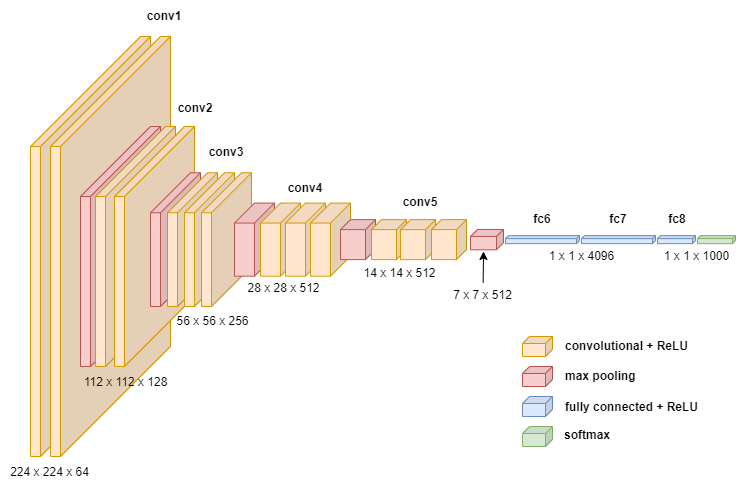
\includegraphics[width=0.75\textwidth]{imgs/vgg16.png}
\caption{VGGNet-16 Architecture. Image Source: \cite{web:NNDiagrams}}\label{fig:vgg-16}
\end{figure}

VGGNet ကို University of Oxford မှ  Visual Geometry Group (VGG) တီထွင်ခဲ့ပြီး ၂၀၁၄ ခုနှစ် ILSVRC ပြိုင်ပွဲတွင် ထူးခြားကောင်းမွန်သည့် ရလဒ်များကို တင်ပြနိုင်ခဲ့သည်။ VGGNet ၏ ထူးခြားချက်မှာ သေးငယ်သော convolutional filter (3x3) ကို အသုံးပြုထားပြီး image ၏ အသေးစိပ် Feature များကို ရှာဖွေခြင်း ဖြစ်သည်။ ထို့အပြင် network တွင် convolutional layer များစွာကို အသုံးပြုသည်။ ယေဘူယျအားဖြင့် VGGNet တွင် convolutional layer အုပ်စု ၅ ခု နှင့် fully connected layer - ၃ ခု တို့ပါ၀င်သည်။  convolutional layer အုပ်စု တစ်ခုတွင် convolutional layer နှစ်ခု (သို့မဟုတ်) သုံးခုအပြင် max-pooling layer တစ်ခုစီလည်း ပါ၀င်သည်။ 

VGGNet architecture တွင် layerတစ်ဆယ့်ခြောက် ခု ပါ၀င်သော VGG16 နှင့် layer တစ်ဆယ့်ကိုးခု ပါ၀င်သော VGG19 ဟု အမျိုးအစား နှစ်မျိုး ရှိသည်။ VGG16 တွင် convolutional layer နှစ်ခု နှင့် max-pooling layer တစ်ခု ပါ၀င်သော အုပ်စု  နှစ်စု၊ convolutional layer သုံးခု နှင့် max-pooling layer တစ်ခု ပါ၀င်သော အုပ်စု  သုံးစု အပြင် fully connected layer - ၃ ခု  ပါ၀င်သည်။ သို့ဖြစ်ရာ VGG16 တွင် ပါ၀င်သည့် စုစုပေါင်း layer အရေအတွက်မှာ (၂ x ၂  + ၃ x ၃ + ၃ = ၁၆) ခု ဖြစ်သည်။ ဤတွက်ချက်မှုတွင် max-pooling layer ကို ထည့်တွက်ခြင်း မပြုထားပါ။ 

\subsection{ResNet (Residual Network)}
ResNet\cite{ResNet_2016}, short for Residual Network, is a type of deep neural network architecture introduced by Kaiming He et al. in 2015. Deep neural networks often suffer from the vanishing gradient problem, where gradients become progressively smaller as they backpropagate from the output layer to the input layer. As a result, earlier layers receive minimal updates, significantly hindering their learning. This problem is common in deep networks, posing a major challenge during training. In addition to vanishing gradients, deep networks can also face the exploding gradient problem, where gradients grow exponentially during backpropagation, leading to model instability. 

\vspace{0.5em}
\begin{figure}[h]%
\centering 
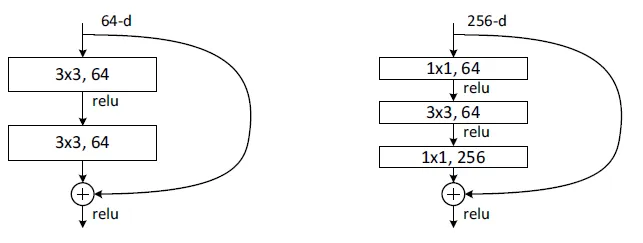
\includegraphics[width=0.85\textwidth]{imgs/res_block.png}
\caption{Residual Blocks. Image Source: \cite{ResNet_2016}}\label{fig:resnet}
\end{figure}

ResNet addresses both the vanishing and exploding gradient problems by introducing shortcut connections, or residual connections, which allow gradients to bypass one or more layers, thereby preserving the gradient flow and stabilizing the training process. The core idea of ResNet is the use of residual blocks (shown in Figure \ref{fig:resnet}), which consist of two or three layers with a direct (shortcut) connection that skips one or more layers. ResNet introduced several versions of the model with varying depths: ResNet-18, ResNet-34, ResNet-50, ResNet-101, and ResNet-152. These models utilize different types of residual blocks to balance between complexity and computational efficiency.

\begin{itemize}[b]
  \item \textbf{Basic Residual Block}(Figure \ref{fig:resnet}-left)), used in ResNet-18 and ResNet-34, consists of 2 layers, typically 3x3 convolutional layers. 
  \item \textbf{Bottleneck Residual Block}(Figure \ref{fig:resnet}-right), used in ResNet-50 and ResNet-101, comprises 3 layers: a 1x1 convolutional layer for dimensionality reduction, a 3x3 convolutional layer, and another 1x1 convolutional layer for restoring the dimensions. 
\end{itemize}

Shallower networks like ResNet-18 and ResNet-34 are faster and less computationally intensive, making them suitable for tasks with limited computational resources. In contrast, deeper networks like ResNet-50 and ResNet-101 can capture more complex patterns, making them better suited for challenging tasks, though they require higher computational resources.

ResNet (သို့မဟုတ်) Residual Network ကို ၂၀၁၅ ခုနှစ်တွင် Microsoft မှ သိပ္ပံပညာရှင် Kaiming He နှင့် အဖွဲ့မှ စတင် တီထွင်ခဲ့ကြသည်။ အထက်တွင် ဆွေးနွေးခဲ့သည့် architecture များကို လေ့လာကြည့်မည် ဆိုပါက model တွင် ပါ၀င်သည့် layer များ ပိုမို များပြားလာသည်နှင့် အမျှ အဆိုပါ architecture ၏ စွမ်းဆောင်ရည်သည် မြင့်တက်လာသည်။ သို့သော် ထိုသို့ layer များ ပိုမိုများလာသည်နှင့်အမျှ parameter များကို update လုပ်သည့် backpropagate လုပ်ငန်းစဥ်တွင် အသုံးပြုသည့် gradient တန်ဖိုးမှာ သေးသည်ထက် သေးလာခြင်း (သို့မဟုတ်) အဆမတန် ကြီးမားလာတတ်သည်။ ဤ ပြဿနာကို  vanishing/exploding gradient problem ဟု ခေါ်ဆိုကြသည်။ ထိုပြဿနာမျိုး ဖြစ်လာပါက အချို့ parameter များသည် တန်ဖိုးမပြောင်းလဲတော့ခြင်း ( gradient တန်ဖိုး သေးလာပါက)၊  အချို့ parameter များ၏ တန်ဖိုးသည် အဆမတန်ကြီးလာနိုင်သည်။ အကျိုးဆက်အားဖြင့် model ၏ စွမ်းဆောင်ရည်များ ကျလာသည်။ 

ResNet သည် အထက်ပါ ပြဿနာများကို ဖြေရှင်းနိုင်ရန်အတွက်  shortcut connection ဟုခေါ်ဆိုသည့် အိုင်ဒီယာ အသစ်တစ်ခုကို တီထွင်ခဲ့ကြသည်။  shortcut connection သည် အချို့ layer များကို အစီအစဥ်အလိုက် မချိတ်ဆက်ဘဲ နှစ်ခု (သို့မဟုတ်) သုံးခုကို ကျော်၍ ချိတ်ဆက်ခြင်းမျိုး ဖြစ်သည်။ ထိုသို့ကျော်၍ ချိတ်ဆက်ထားသည့် layer များ ပါ၀င်သည့် အုပ်စု တစ်ခုကို residual block ဟု ခေါ်ဆိုကြသည်။ ResNet version အမျိုးမျိုး ရှိပြီး model တွင် ပါ၀င်သည့် layer အရေအတွက်ကို အခြေခံ၍ ResNet-18, ResNet-34, ResNet-50, ResNet-101, နှင့် ResNet-152 စသည်ဖြင့် ခေါ်ဆိုကြသည်။ 

ResNet-18 တွင် အထက်ပါပုံ (ဘယ်ဘက်) တွင် ပြသထားသည့်  residual block ရှစ်ခု ပါ၀င်ပြီး စုစုပေါင်း layer  (၁၈) ခု ပါ၀င်သည်။ ResNet-18 နှင့် ResNet-34 တွင် အသုံးပြုသည့် residual block တွင် layer နှစ်ခုပါ၀င်ပြီး များသောအားဖြင့် 3x3 convolutional filter များကို အသုံးပြုသည်။ ResNet-50, ResNet-101, နှင့် ResNet-152 တို့တွင် အသုံးပြုသည့် residual block (ပုံ \ref{fig:resnet}  ညာဘက်) တွင်မူ layer သုံးခုပါ၀င်ပြီး 1x1 convolutional layer ကို block ၏ အစနှင့် အဆုံးတွင် အသုံးပြုထားသည်။ layer နည်းသည့် ResNet-18 နှင့် ResNet-34 တို့ကို computational resource အများကြီး မလိုအပ်သည့် လုပ်ငန်းစဥ်များအတွက် အသုံးပြုနိုင်ပြီး  computational resource  ပိုမို လိုအပ်သည့် ကျန် deep ResNet များကို ခက်ခဲသည့် လုပ်ငန်းစဥ်များအတွက် အသုံးပြုနိုင်သည်။ 


\subsection{GoogLeNet (Inception)} 
GoogLeNet \cite{GoogleNet2015}, also known as Inception v1, is developed by researchers at Google. It was introduced in 2014 as part of the ImageNet Large Scale Visual Recognition Challenge (ILSVRC).  The key innovation of GoogLeNet is its use of the Inception module. This module is designed to capture different types of features by applying convolutions of various sizes (1x1, 3x3, 5x5) and a pooling operation (typically max pooling) in parallel, as shown in Figure\ref{fig:inception}. The outputs of these operations are concatenated along the depth dimension, enabling the network to capture multi-scale features. While increasing the depth and width of the network, GoogLeNet maintains computational efficiency.

\vspace{0.5em}
\begin{figure}[h]%
\centering 
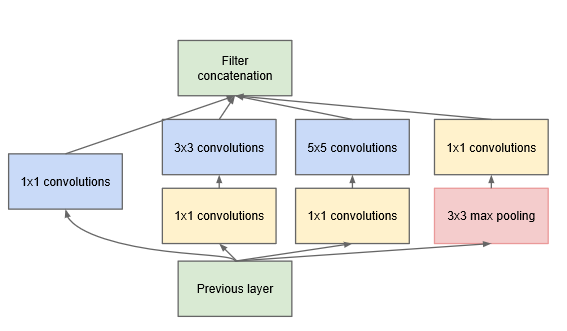
\includegraphics[width=0.55\textwidth]{imgs/inception1.png}
\caption{Inception module. Image source \cite{GoogleNet2015}}\label{fig:inception}
\end{figure}

GoogLeNet consists of nine inception blocks, each containing two layers of inception modules. In total, the network includes 22 layers with parameters, or 27 layers when including the pooling layers.Following G oogleNet (Inception v1), several improved versions have been introduced, such as:
\begin{itemize}[b]
  \item \textbf{Inception v2 and v3}: Introduce batch normalization, factorized convolutions, and other improvements to enhance training and performance.
  \item \textbf{Inception v4 and Inception-ResNet}: Combine Inception modules with residual connections, further improving training efficiency and model accuracy.
\end{itemize}

GoogLeNet (သို့မဟုတ်) Inception v1 ကို ၂၀၁၄ ခုနှစ်တွင်  Google မှ သုတေသနပညာရှင်များက တီထွင်ခဲ့ပါသည်။ အဆိုပါ GoogLeNet ၏ ထူးခြားချက်မှာ အထက်ပါ ပုံတွင် ပြသထားသည့် Inception module ဖြစ်သည်။ 
ပုံရိပ်တစ်ခုတွင် ပါ၀င်သည့် အရေးကြီးသော object ၏ အရွယ်အစားမှာ အမျိုးမျိုး ဖြစ်နေနိုင်ရာ မတူညီသည့် filter size များကို အသုံးပြုခြင်းဖြင့် အမျိုးအစားခွဲခြားရာတွင် အသုံး၀င်သည့် feature များကို ရှာဖွေနိုင်သည်။ GoogLeNet မတိုင်မီ တီထွင်ခဲ့သည့်  Convolutional Neural Network များကို လေ့လာကြည့်မည်ဆိုပါက layer အရေအတွက်  များလာသည်နှင့် အမျှ ပိုမိုကောင်းမွန်သည့် ရလဒ်များကို ရရှိသည်ကို တွေ့ရှိနိုင်သည်။ သို့သော် layer အရေအတွက်  များလာသည်နှင့် အမျှ model ကို Training ပြုလုပ်ရန် အသုံးပြရသည့် ကြာချိန် ပိုလာပြီး computational resource များလည်း ပိုမို လိုအပ်လာသည်။ 

GoogLeNet တွင် ပါ၀င်သည့် Inception module ၏ ထူးခြားချက်မှာ Neural network တစ်ခုတွင်  layer အရေအတွက် ထပ်တိုးရမည့် အစား Layer တစ်ခုထဲတွင် convolution filter size သုံးမျိုးကို အသုံးပြု၍ feature များကို ရှာဖွေခြင်း ဖြစ်သည်။  GoogLeNet တွင် inception block - ၉ ခု ပါ၀င်ပြီး အဆိုပါ  inception block - တစ်ခု၌ ပုံ \ref{fig:inception} တွင် ပြသထားသည့် Inception module နှစ်ခုစီ ပါ၀င်သည်။ ထို့အပြင် convolutional layer များလည်း ပါ၀င်ရာ GoogLeNet ၏ architecture တွင် layer စုစုပေါင်း နှစ်ဆယ့်နှစ်ခု ပါ၀င်သည်။ Pooling Layer များကိုပါ ထည့်သွင်းစဥ်းစားမည်ဆိုပါက layer နှစ်ဆယ့်ခုနစ် ခု ပါ၀င်သည်။ GoogLeNet တွင် fully-connected-layer များအစား average pooling layer နှင့် drop-out layer တို့ကို တွဲ၍ အသုံးပြုထားသည်။ drop-out layer ဆိုသည်မှာ အဆိုပါ layer ရှိ neuron များအနက် ရာခိုင်နှုန်းအချို့ကို ယာယီ ထည့်သွင်း မစဥ်းစားခြင်း ဖြစ်သည်။ GoogLeNet ၏ architecture တွင် rectified linear activation function ကို အသုံးပြုထားသည်။ 

ယနေ့ အချိန်တွင် GoogLeNet ကို အခြေခံသည့် Inception v2 ၊ v3 ၊  v4 နှင့် GoogLeNet နှင့် ResNet တို့ကို ပေါင်းစည်းထားသည့် Inception-ResNet တို့ကို တီထွင်ခဲ့ကြပြီး ဖြစ်သည်။  

\subsection{EfficientNet}

\newpage
\subsection{ConvNeXt}
\newpage


\subsection{Evolution of CNN}

The evolution of Convolutional Neural Networks (CNNs) represents a significant advancement in computer vision, with each architecture improving on previous designs to address specific challenges. This section discussed key architectures such as ConvNet, AlexNet, ResNet, GoogLeNet, EfficientNet, and ConvNext, which form the basis for modern methodologies in object detection and image classification.

YOLO (You Only Live Once) exemplifies the application of these advancements, achieving state-of-the-art performance in real-time object detection. By building on the principles of earlier CNN models, YOLO optimizes for speed and accuracy, revolutionizing various industries and driving innovation in computer vision applications.

ယခု အခန်းတွင် ဆွေးနွေးခဲ့သည့် CNN Architecture အမျိုးမျိုးကို လေ့လာကြည့်ပါက သုတေသန ပညာရှင်များသည် တစ်နှစ်ထက် တစ်နှစ်ထက် ပိုမိုကောင်းမွန်သည့် model များ ထွက်ပေါ်လာရန် ကြိုးစားလာနေသည်ကို တွေ့နိုင်ပါသည်။  ယခု အခန်းတွင် ဆွေးနွေးခဲ့သည့် architecture များအပြင်  CNN architecture အသစ်များသည် အချိန်နှင့် အမျှ ထွက်ပေါ်လာနေသည်။ အဆိုပါ Architecture များ၏ တိုးတက်မှုသည် object detection နှင့် image classification စသည့် computer vision လုပ်ငန်းစဥ် အမျိုးမျိုးကို များစွာ အထောက်အပံ့ဖြစ်သည်။ 

Real time object detection လုပ်ငန်းစဥ်ကို ဆောင်ရွက်ပေးသည့် YOLO (You Only Live Once)  သည် အဆိုပါ ပြောင်းလဲမှုများ၏ တိုးတက်မှု အကျိုးကျေးဇူးကို သိသာထင်ရှားစေသော ဥပမာ တစ်ခုပင် ဖြစ်သည်။ YOLO version များသည် နှစ်စဥ် အသစ်ထွက်ပေါ်လာလျက် ရှိပြီး နောက်ဆုံး ထွက်ပေါ်လာသည့် YOLO v9 သည် accuracy တိုးတက်လာရုံမက computational resources ကို လည်း လျော့ချပေးနိုင်သည်ဟု အဆိုပြုထားကြသည်။ 


\newpage
\section{Datasets for Computer Vision Tasks}
In the field of computer vision, several datasets \cite{web:cvDatasets} have become essential benchmarks for various tasks such as image classification, object detection, and segmentation. The most commonly used datasets are listed below:
\begin{itemize}[b] 
\item \textbf{ImageNet}:  ImageNet \cite{web:ILSVRC} is one of the largest image datasets available, containing over 14 million labeled images across 20,000 categories. It is primarily used for image classification and object recognition tasks. The ImageNet Large Scale Visual Recognition Challenge (ILSVRC) has driven significant advancements in the field of deep learning and computer vision. Models like AlexNet, VGG, ResNet, and GoogLeNet were benchmarked on this dataset. Some sample images from ImageNet are shown in Figure \ref{fig:imgNet}.
    \item \textbf{Pascal VOC}: PASCAL Visual Object Classification (PASCAL VOC) 2007 and 2012 \cite{web:Pascal} is a familiar and widely used dataset for object detection object detection, classification, and segmentation. It includes a series of yearly challenges with datasets that feature annotated objects across 20 different categories.
    \item \textbf{COCO}: The common Objects in COntext (COCO) dataset \cite{web:CoCo} was developed by Microsoft team. It is a large-scale dataset for object detection, segmentation, and captioning. It contains over 330,000 images with more than 1.5 million object instances, labeled with 80 object categories.
    \item \textbf{Open Images Dataset}: Open Images \cite{web:OpenImage} is a large-scale dataset for object detection, image classification, and visual relationship detection. The dataset contains about 9.2 million labeled and unified ground-truth images and segmentation masks. This database has about 600 object classes with almost 16 million bounding boxes. It is considered one of the largest databases for object localization.
\end{itemize}

\vspace{0.5em}
\begin{figure}[h]%
\centering
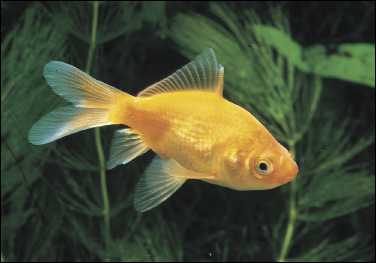
\includegraphics[width=0.25\textwidth]{imgs/imgnet_1.jpeg}
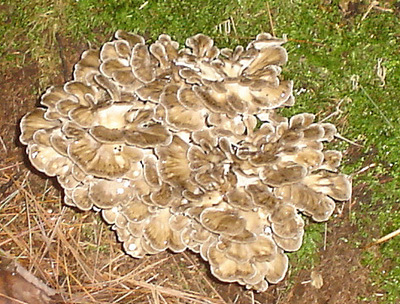
\includegraphics[width=0.25\textwidth]{imgs/imgnet_2.jpeg}
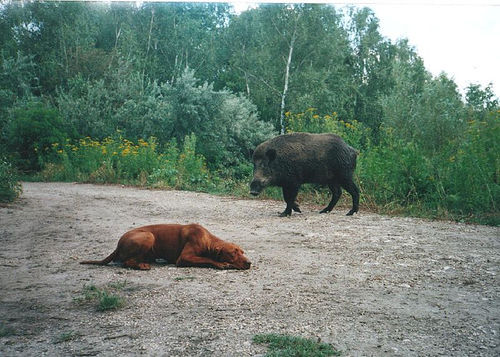
\includegraphics[width=0.25\textwidth]{imgs/imgnet_3.jpeg}
\caption{Sample images from ImageNet\cite{web:ILSVRC}}\label{fig:imgNet}
\end{figure}

Computer vision ဘာသာရပ်တွင် ယုံကြည်စိတ်ချရသော dataset များသည် AI model များ တီထွင်ဖန်တီးနိုင်ခြင်း၏ အသက်ဖြစ်သည်။ သို့သော် အဆိုပါ datasetများကို ဖန်တီးတည်ဆောက်ရန်မှာ မလွယ်ကူပါ။ Computer vision ဘာသာရပ်တွင် အသုံးများသည့် datasetများမှာ အောက်ပါအတိုင်း ဖြစ်သည်။ 

\begin{itemize}[b] 
\item \textbf{ImageNet}:  ImageNet \cite{web:ILSVRC} တွင် ကား၊ ပရိဘောဂ၊ အ၀တ်အစား၊ အစားအသောက် စသည်ဖြင့် အမျိုးအစားပေါင်း ၂ သောင်း၏ image စုစုပေါင်း တစ်ဆယ့် လေးသန်းကျော်ပါ၀င်သည်။ Image classification နှင့် object recognition လုပ်ငန်းစဥ်များ၊ပြိုင်ပွဲများတွင် အများဆုံး အသုံးပြုခဲ့ကြသည့် dataset လည်းဖြစ်သည်။ ImageNet Large Scale Visual Recognition Challenge (ILSVRC)  ပြိုင်ပွဲကို ၂၀၁၀ မှ ၂၀၁၇ အထိ နှစ်စဥ် ကျင်းပခဲ့ကြပြီး ILSVRC တွင် အမျိုးအစားပေါင်း တစ်ထောင် ၏ ဓါတ်ပုံ တစ်ဆယ့်နှစ်သန်းကျော်ပါ၀င်သည့်  dataset ကို အသုံးပြုယှဥ်ပြိုင်ခဲ့ကြသည်။ အထက်တွင် ဆွေးနွေးခဲ့သည့် AlexNet, VGG, ResNet, နှင့် GoogLeNet တို့တွင် ၄င်းတို့၏ စွမ်းဆောင်ရည်ကို တိုင်းတာနိုင်ရန် ဤ dataset ကို အသုံးပြုခဲ့ကြသည်။ 
    \item \textbf{Pascal VOC}: PASCAL Visual Object Classification (PASCAL VOC) 2007 and 2012 \cite{web:Pascal} သည်လည်း လူသုံးများသည့် အခြား dataset တစ်ခု ဖြစ်သည်။ ဤ datasetကို အသုံးပြု၍ နှစ်စဥ်ပြိုင်ပွဲ ပြုလုပ်လေ့ရှိပြီး ကား၊ လေယာဥ်ပျံ၊ စက်ဘီး၊ ငှက်၊ လှေစသည်ဖြင့် အမျိုးအစားပေါင်း ၂၀ ကျော်၏  image စုစုပေါင်း ၃ ထောင်ကျော်ပါ၀င်သည်။ 
    \item \textbf{COCO}: Microsoft အဖွဲ့မှ ထုတ်လုပ်သည့် COCO) dataset \cite{web:CoCo}တွင် မတူညီသည့် အမျိုးအစားပေါင်း ၈၀ အတွက်   image စုစုပေါင်း သုံးသိန်း သုံးသောင်းကျော် ပါ၀င်သည်။ 
    \item \textbf{Open Images Dataset}: Open Images \cite{web:OpenImage} သည် နောက်ဆုံး ထွက်ထားသည့် dataset ဖြစ်ပြီး image စုစုပေါင်း ကိုးသန်း နှစ်သိန်းကျော်ပါ၀င်သည်။ မတူညီသည့် အမျိုးအစား - ၆၀၀ ကျော်ပါ၀င်ပြီး image အတွင်ရှိ object ၏ နေရာကို အတိအကျပေးထားသည့် bounding box ၁၆ သန်းပါ၀င်သည်။ 
\end{itemize}

\newpage
\section{Case Study: Image Classification}

This section presents two distinct case studies showcasing the application of deep learning in image classification. The first project explores object classification using various CNN architectures discussed in section \ref{sec:vCNN}, while the second delves into handwritten digit recognition. Both projects aim to leverage deep learning techniques to solve practical image classification tasks.

ဤအခန်းတွင် လက်တွေ့ သင်ခန်းစာများအဖြစ် project - နှစ်ခုကို တင်ပြထားသည်။ ပထမ project မှာ အထက်၌ တင်ပြထားခဲ့သည့် CNN architecture များကို အသုံးပြု၍ image များကို အမျိုးအစား ခွဲခြင်းခြင်းဖြစ်ပြီး ဒုတိယ project တွင်မူ လက်ရေးဖြင့် ရေးထားသော သင်္ချာ ကိန်းဂဏန်းများကို အလိုအလျောက်ခွဲခြားပေးနိုင်မည့် deep learning architecture တစ်ခု တည်ဆောက်ရန် ဖြစ်သည်။ 

\subsection{Case Study-1: Object Classification using different CNN architectures}

In this project, AI-generated images are classified using five  state-of-the-art Convolutional Neural Network (CNN) models implemented with the Python `keras` library. The models used are `\texttt{ResNet50}`, `\texttt{VGG16}`, `\texttt{InceptionV3}`, `\texttt{ConvNeXtTiny}`, and `\texttt{EfficientNetB7}`. The goal is to load an image, pass it through each of these models, and obtain the top prediction for the image as shown in Figure \ref{fig:p1R}. 

This project consists of two Python scripts: one for defining the CNN models (`\texttt{cnn\_models.py}`) and one main script (`\texttt{main.py}`) for classifying an image.

\vspace{0.5em}
\begin{figure}[h]%
\centering 
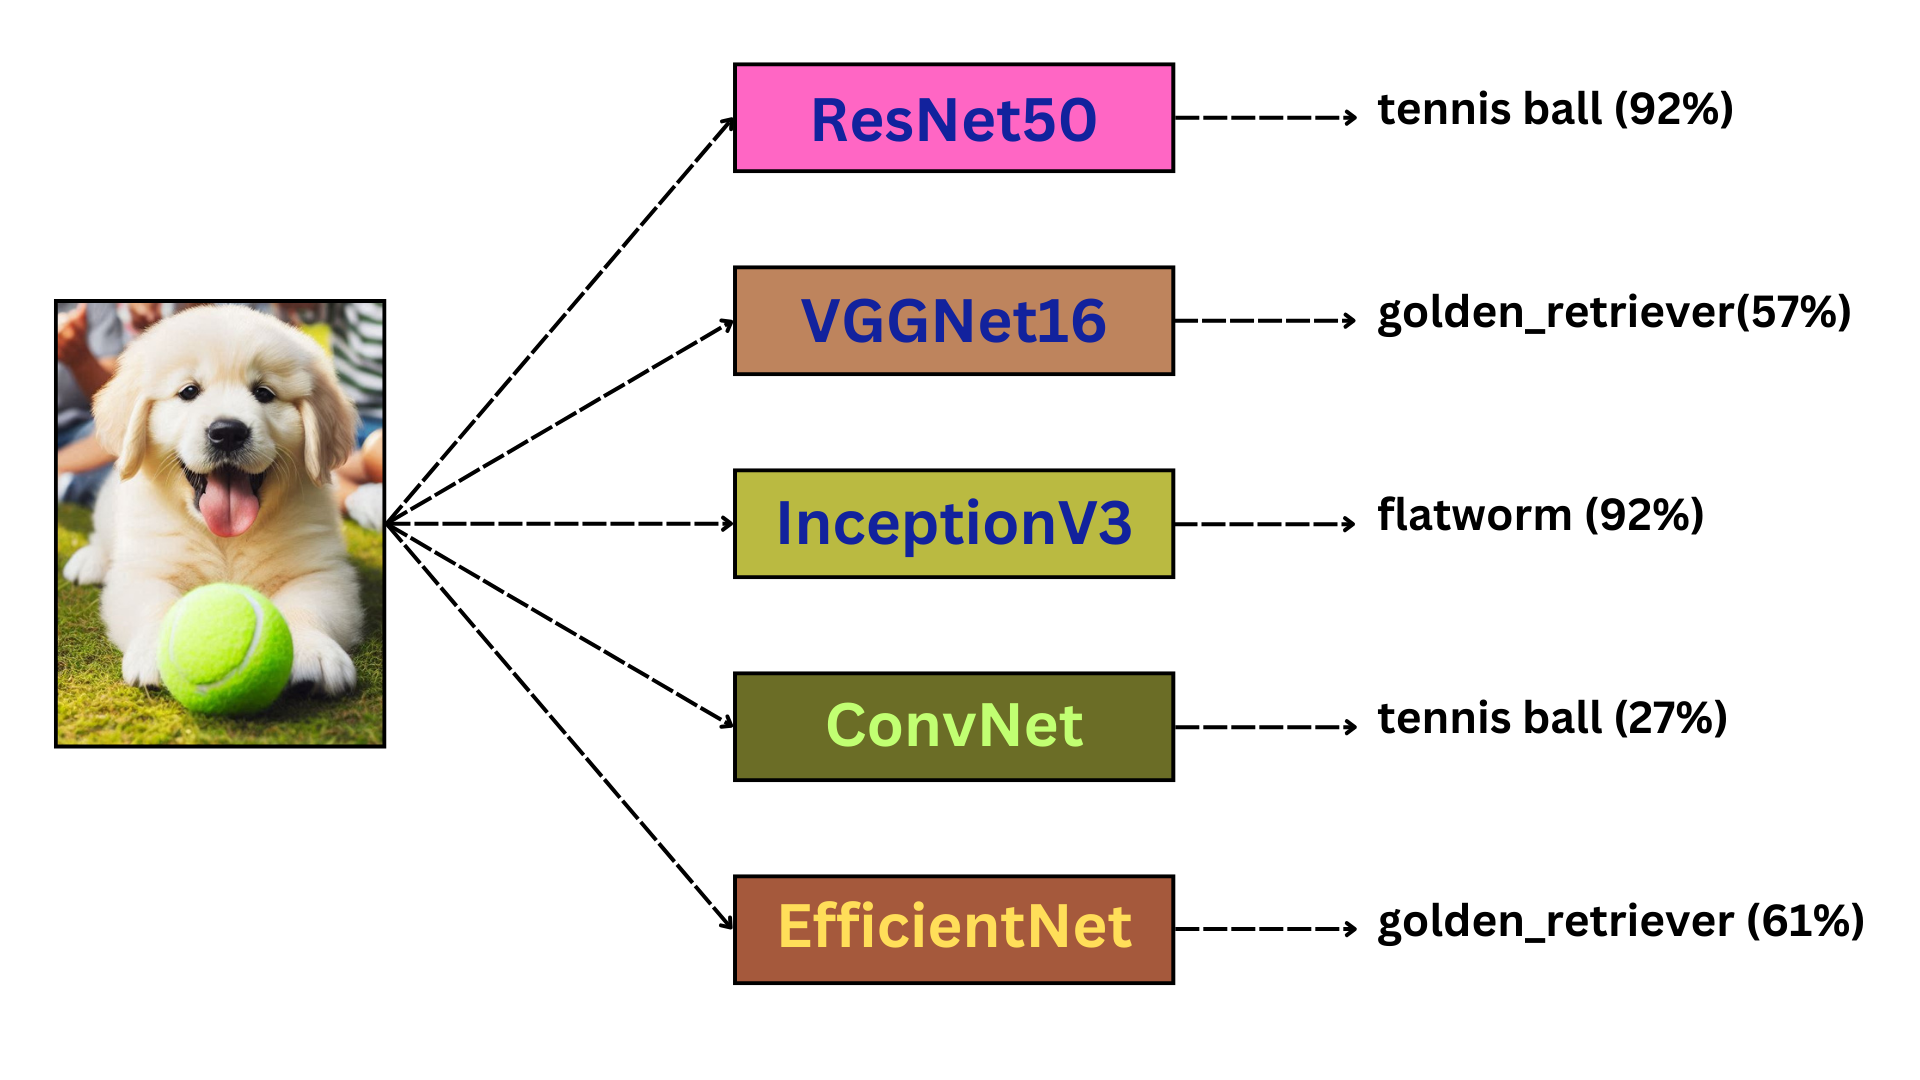
\includegraphics[width=0.8\textwidth]{imgs/p1_result.png}
\caption{Prediction of Objects by 5 different state-of-the-art CNN architectures}\label{fig:p1R}
\end{figure}

ပထမ project မှာ အခန်း \ref{sec:vCNN} တွင် ဆွေးနွေးခဲ့သည့် CNN architecture များအနက် - ငါးခုကို အသုံးပြု၍ AI ဖြင့် ဖန်တီးယူထားသည့် ပုံရိပ်များကို အမျိုးအစား ခွဲခြားခြင်း ဖြစ်သည်။ ယခု project တွင် အသုံးပြုမည့်  CNN architecture များမှာ  `\texttt{ResNet50}`, `\texttt{VGG16}`, `\texttt{InceptionV3}`, `\texttt{ConvNeXtTiny}`, နှင့် `\texttt{EfficientNetB7}`တို့ ဖြစ်ကြသည်။ 

ယခု  project တွင် (`\texttt{cnn\_models.py}`) နှင့် (`\texttt{main.py}`) ပါ၀င်သည်။ ပထမ  script  (`\texttt{cnn\_models.py}`) ၍ Python `keras` library တွင် pre-trained ပြုလုပ်ထားပြီး ဖြစ်သည့် CNN model များကို ခေါ်ယူ အသုံးပြုရန် ရေးထားသည့် class ဖြစ်သည်။ အဆိုပါ class တွင် ခေါ်ယူ အသုံးပြုမည့် CNN architecture များ၏ အမည်ကို သတ်မှတ်သည့် function ၊ CNN architecture များကို initialize လုပ်သည့် function များနှင့် input image ကို classify လုပ်မည့် function များ ပါ၀င်သည်။ 

ဒုတိယ script (`\texttt{main.py}`)  သည် (`\texttt{cnn\_models.py}`) ကို အသုံးပြု၍ ပုံရိပ်တစ်ခုကို ခွဲခြားပေးသည်။ 

\newpage
\subsubsection{Python Implementation}

\begin{itemize}[b]
\item{ \texttt{`cnn\_models.py`}}: This script defines a class, \texttt{`cnnModels`}, which provides an interface to load and use the pre-trained CNN models. The class includes methods for initializing models, retrieving models by name, and classifying images.

\item{\texttt{ `main.ipynb`}}: This script demonstrates how to use the `cnnModels` class to classify an image.
\end{itemize}

\begin{solution}
\begin{lstlisting}
    class cnnModels:
        def __init__(self):
            self.models = {'ResNet50': self.resnet(), 'VGGNet16': self.vggnet(), 
                           'InceptionV3': self.inception(), 'ConvNet': self.convnet(), 
                           'EfficientNet': self.efficientnet()}
    
        def resnet(self):       
            model = ResNet50(weights='imagenet')
            return model
        
        def vggnet(self):
            model = keras.applications.VGG16(weights='imagenet')
            return model
        
        def inception(self):
            model = keras.applications.InceptionV3(weights='imagenet')
            return model
        
        def convnet(self):
            model = keras.applications.ConvNeXtTiny(weights='imagenet')
            return model       
        
        def efficientnet(self):
            model = keras.applications.EfficientNetB7(weights='imagenet')
            return model
    
        def get_model(self, name):
            if name in self.models:
                return self.models[name]
            else:
                raise ValueError(f"Model '{name}' does not exist.")            
            
        def classify_image(self, name, img):
            model = self.get_model(name)      
            
            img = img.resize((model.input_shape[1], model.input_shape[2]))  
            x = img_to_array(img)
            x = np.expand_dims(x, axis=0)
            x = preprocess_input(x)
            
            preds = model.predict(x)
            return decode_predictions(preds, top=1)

\end{lstlisting}  
\end{solution}

\begin{solution}
\begin{lstlisting}
    from cnn_models import cnnModels
    from keras.preprocessing.image import load_img
    
    img_path = './imgs/dog.jpeg'
    img = load_img(img_path)
    
    model = cnnModels()    
    preds1 = model.classify_image('ResNet50', img)
    
    for pred in preds1:
        print(f"{pred[1]}: {pred[2]}, {pred[3]}")
\end{lstlisting}

\end{solution}
\vspace{0.5em}
\begin{figure}[h]%
\centering 
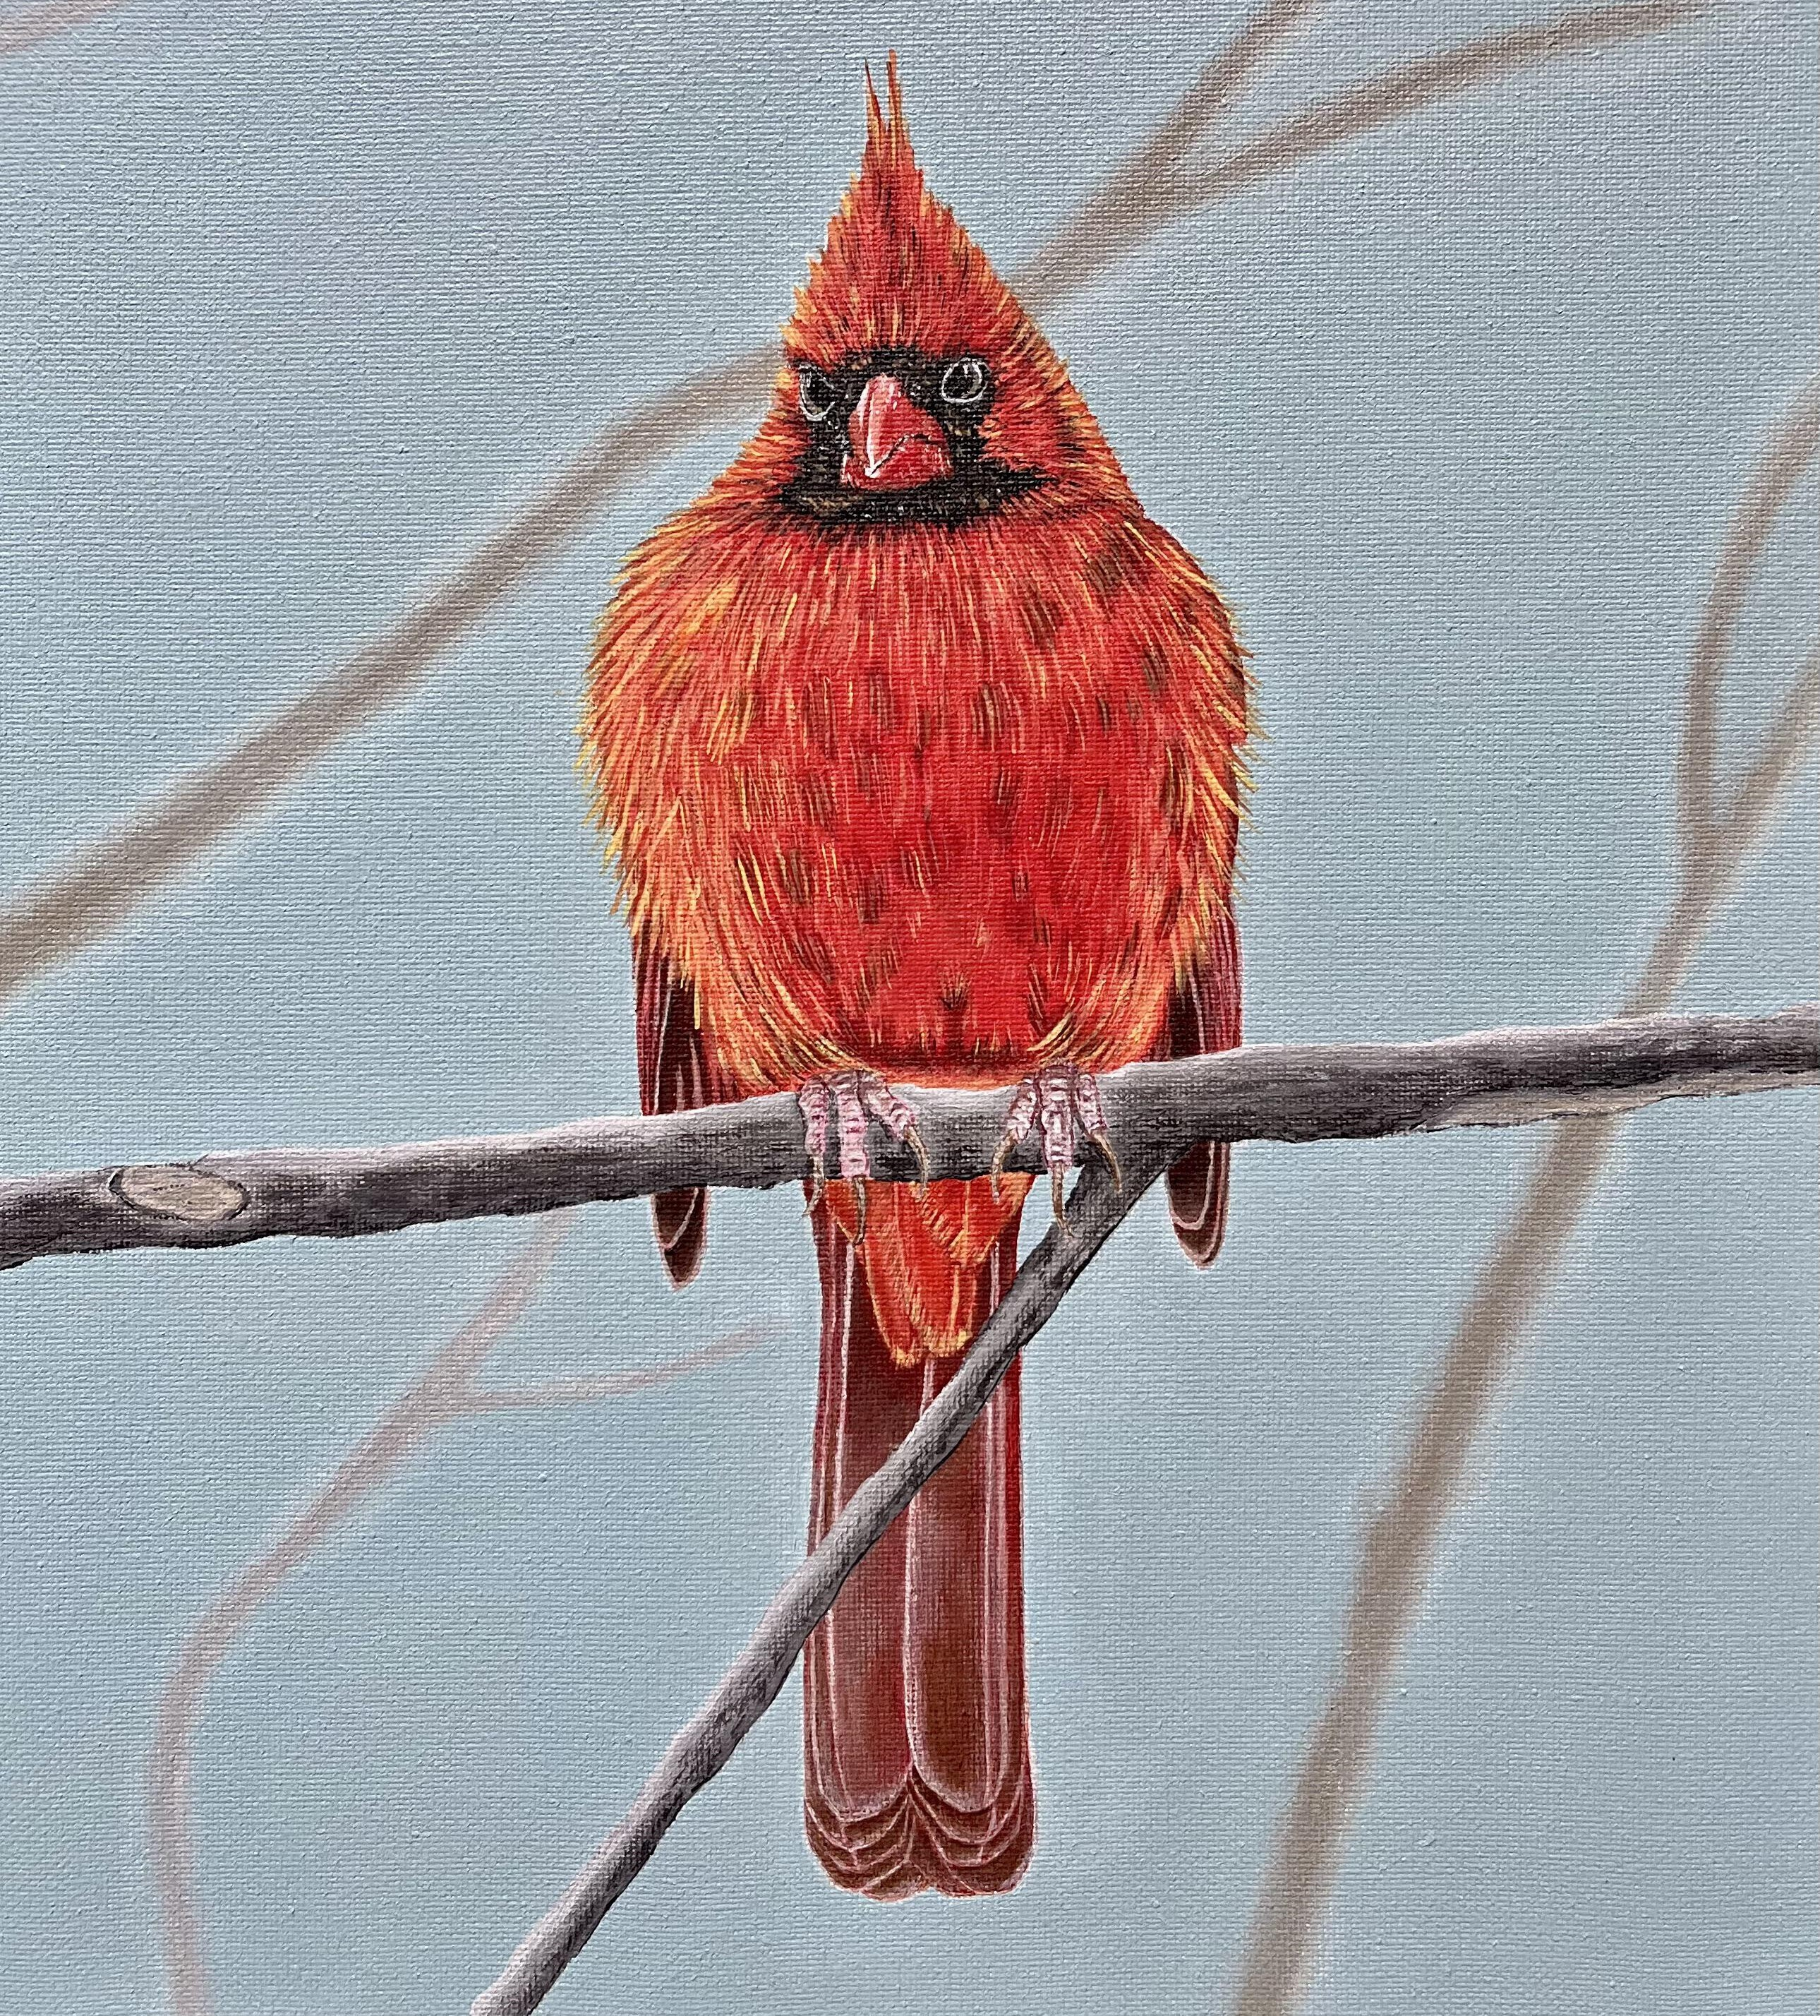
\includegraphics[width=0.23\textwidth]{imgs/bird.jpg}
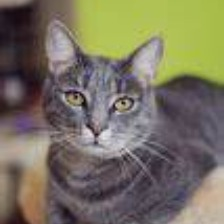
\includegraphics[width=0.24\textwidth]{imgs/cat.jpg}
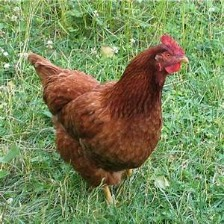
\includegraphics[width=0.24\textwidth]{imgs/chicken.jpg}
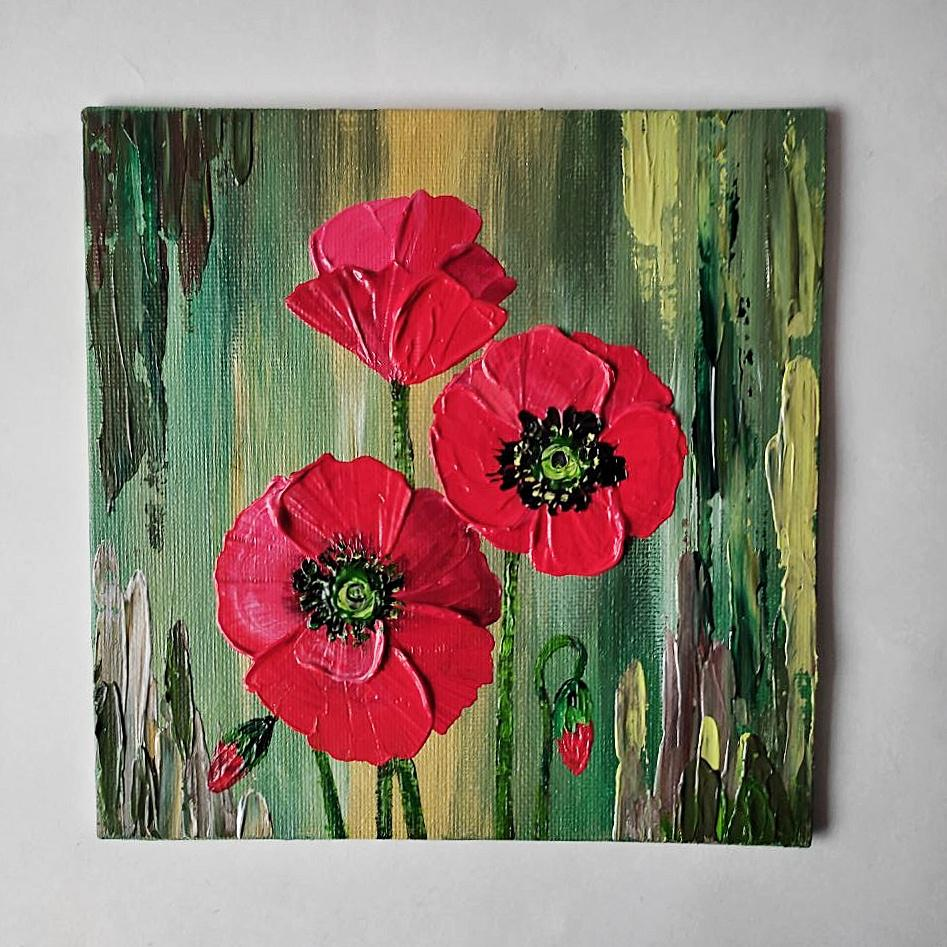
\includegraphics[width=0.24\textwidth]{imgs/flower.jpg}

\includegraphics[width=0.24\textwidth]{imgs/bird.jpeg}

\includegraphics[width=0.24\textwidth]{imgs/cat.jpeg}
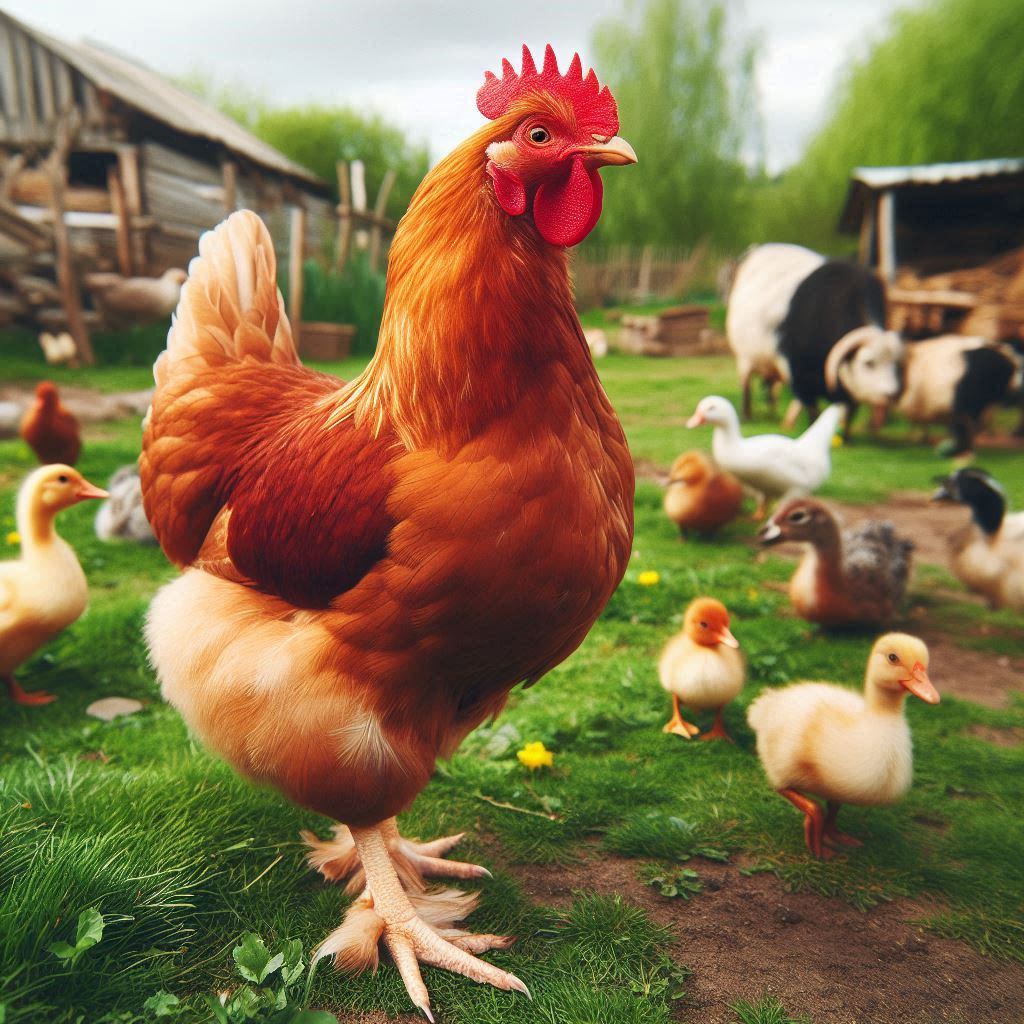
\includegraphics[width=0.24\textwidth]{imgs/chicken.jpeg}

\includegraphics[width=0.24\textwidth]{imgs/rose.jpeg}
\caption{Sample Images. The first row displays real images collected from the internet, whereas the second row shows synthetic images generated using AI.}\label{fig:p1R}
\end{figure}
\subsubsection{Dataset}
In this project, a small dataset comprising 20 images is utilized. This dataset includes 10 real images collected from the internet and 10 synthetic images generated using Microsoft Image Generator \cite{web:MSimgCreator}. The sizes of the real images are random, while the synthetic images have a fixed dimension of 1024 x 1024 pixels. These images are pre-processed before being fed into the cnnModel module explained above.

ဤ project တွင် real image တစ်ဆယ်ခုနှင့် AI အသုံးပြု၍ ဖန်တီထားသည့် ပုံရိပ် ဆယ်ခုတို့ကို အသုံးပြု၍ image classification ပြုလုပ်ပြသွားမည်ဖြစ်သည်။ real image များမှာ အင်တာနက်မှ ရယူထားခြင်းဖြစ်ရာ ၄င်းတို့၏ image size မှာ 214 x 214 မှ 2567x 2586 အထိ အမျိုးမျိုး ပါ၀င်သည်။ AI အသုံးပြု၍ ဖန်တီထားသည့် ပုံရိပ်များ၏ image size မှာ 1024 x 1024 ဖြစ်သည်။ အထက်တွင် ဖော်ပြထားသည့် cnnModel module ကို အသုံးပြု၍ image များကို အမျိုးအစားမခွဲခြားမီ သက်ဆိုင်ရာ CNN model များမှ လိုအပ်သည့် အရွယ်အစားကို ရအောင် ညှိပေးရမည် ဖြစ်သည်။ ဥပမာ  VGGNet နှင့် ResNet Model များအတွက် input image ၏ အရွယ်အစားမှာ 224 x 224 ဖြစ်သည်။ 

\subsubsection{Results and Discussion}

\newpage
\subsection{Case Study-2: Handwritten Digit Recognition}
Handwritten digit recognition is a classic problem in computer vision and machine learning, involving training a model to classify handwritten digits (0-9) from images. While numerous solutions exist for English digit recognition, there's a limited resources for recognizing digits in languages like Myanmar. The objective of this project is to bridge this gap by developing a machine learning model capable of recognizing handwritten digits in the Myanmar language. This task holds significant importance for various applications, including digitization efforts, character recognition systems, and automation technologies. However, Myanmar script presents unique challenges, such as variations in writing styles, stroke thickness, and complex shapes, making digit recognition a non-trivial task. Therefore, the development of an efficient architecture tailored to address these challenges is crucial for the advancement of the Myanmar community in the journey of technology.

လက်ရေးဖြင့် ရေးထားသော နံပါတ်များကို ကွန်ပြူတာမှ နားလည်စေရန် လေ့ကျင့်ပေးသည့် လုပ်ငန်းစဥ်သည် computer vision လောကတွင် အရေးကြီးသည့် ပြဿနာတစ်ခုဖြစ်ပြီး Method ပေါင်းများစွာ တီထွင်ခဲ့ကြပြီး ဖြစ်သည်။ ဤ လုပ်ငန်းစဥ်သည် လက်ရေးဖြင့် ရေးထားသော စာရွက်စာတမ်းများကို ကွန်ပြူတာဖြင့် သိမ်းဆည်းနိုင်ရန် အတွက် အရေးကြီးသော အဆင့်တစ်ခု ဖြစ်သည်။ အင်္ဂလိပ် ဘာသာစကားဖြင့် ရေးသားထားသော နံပါတ်များကို ကွန်ပြူတာမှ နားလည်စေရန် လေ့ကျင့်ပေးထားသော AI tool များစွာ ရှိသော်လည်း မြန်မာ ဘာသာဖြင့် ရေးသားထားသော ဂဏန်းများအတွက် လေ့ကျင့်ပေးထားသော Programme သည် အကန့်အသတ်ဖြင့်သာ ရှိနေသေးသည်။ မြန်မာ နံပါတ်များသည် တမူကွဲပြားသည့် ရေးဟန် ရှိရာ မြန်မာ ဘာသာစကားအတွက် သီးသန့် ရည်ရွယ်သည့် Method များထွက်ပေါ်လာရန် လိုအပ်သည်။ ယခု Project တွင် လက်ရေးဖြင့်ရေးသားထားသည့် မြန်မာ နံပါတ်များကို နားလည်နိုင်ရန်အတွက် CNN ကို အခြေခံသည့် deep learning model တစ်ခု တည်ဆောက်သွားမည် ဖြစ်သည်။ 

\subsubsection{Dataset}
In handwritten digit recognition, the MNIST dataset \cite{web:mnist} is a commonly used benchmark, featuring 28x28 grayscale images of English handwritten digits. However, the MNIST dataset is limited to digits written in English. In this project, we utilized a dataset from \cite{web:MMdataset}, containing 2,200 images of Myanmar handwritten digits, with each digit represented by 220 images. Some sample images are shown in Figure \ref{fig:p2MMdigits}. Seventy percent of the images (1,540) were used for training, while the remaining 30 percent (660) were reserved for testing.

လက်ရေးဖြင့် ရေးထားသည့် နံပါတ်များနှင့် ပတ်သတ်သည့် Project များ ပြုလုပ်ရာတွင် ၁၉၉၈ ခုနှစ်က သုတေသနပညာရှင် Yann LeCun နှင့် အဖွဲ့ ထုတ်ခဲ့သည့်  MNIST dataset ကို အများဆုံး အသုံးပြုကြသည်။ အဆိုပါ dataset သည်  အင်္ဂလိပ် ဘာသာစကားဖြင့် ရေးသားထားသော နံပါတ်များအတွက် အကောင်းဆုံး ဖြစ်သော်လည်း မြန်မာဘာသာဖြင့် ရေးထားသည့် နံပါတ်များ မပါ၀င်ပါ။ သို့ဖြစ်ရာ ဤ Project တွင် မြန်မာ လူငယ်များ စုစည်းထားသည့် လက်ရေးဖြင့်ရေးထားသည့် မြန်မာ နံပါတ်များပါ၀င်သည့် dataset ကို အသုံးပြုခဲ့သည်။ အဆိုပါ dataset တွင် နံပါတ် တစ်ခုစီအတွက် image နှစ်ရာ့ နှစ်ဆယ်စီ ပါ၀င်ရာ image စုစုပေါင်း နှစ်ထောင့်နှစ်ရာ ပါ၀င်သည်။ ထိုအထဲမှ ခုနစ်ဆယ် ရာခိုင်နှုန်းကို training အတွက် အသုံးပြုခဲ့ပြီး ကျန် သုံးဆယ် ရာခိုင်နှုန်းကို testing အတွက် အသုံးပြုထားသည်။ ဤ dataset တွင် ပါ၀င်သည့် နမူနာ image အချို့ကို အောက်တွင် ပြသထားသည်။ 

\vspace{0.5em}
\begin{figure}[h]%
\centering 

\includegraphics[width=0.15\textwidth]{imgs/0.jpg}

\includegraphics[width=0.15\textwidth]{imgs/1.jpg}

\includegraphics[width=0.15\textwidth]{imgs/2.jpg}

\includegraphics[width=0.15\textwidth]{imgs/3.jpg}

\includegraphics[width=0.12\textwidth]{imgs/4.jpg}
\caption{Sample Images of Myanmar handwritten digits.}\label{fig:p2MMdigits}
\end{figure}

\subsubsection{Data Preprocessing}
The images of handwritten digits are initially provided as 310x219 gray-scale matrices. Since the region of interest (the handwritten digit) is relatively small, approximately 80x80 pixels and centered, the first step in data preprocessing is to \texttt{crop} the image by removing 50 pixels from the left and right, and 20 pixels from the top and bottom. This results in an image size of 270x179 pixels. 

Next, to prepare the images for input into the proposed deep learning architecture, the cropped images are \texttt{resized} to 64x64 pixels. This resizing step ensures uniformity in the input data dimensions, which is crucial for effective processing by the neural network. By reducing the image dimensions, the model can focus on the essential features of the handwritten digits, improving both efficiency and performance in training and evaluation.

Furthermore, an additional dimension is needed for the Convolutional Neural Network (CNN) model. Therefore, the resized images are \texttt{reshaped} to have a shape of $(Nx 64x 64x 1)$, where N is the number of images. This reshaping ensures that the data is in the correct format, with the final dimension representing the single channel of the gray-scale images.

ဤ Project အတွက် အသုံးပြုသည့် dataset ရှိ  image ၏ အရွယ်အစားမှာ 310x219 ဖြစ်ပြီး gray-scale image များဖြစ်ကြသည်။ သို့သော် image တွင် ပါ၀င်သော နံပါတ်များသည် image ၏ အလယ်လောက် တွင် ရှိပြီး နံပါတ်သည် image ၏ အရွယ်အစား နှင့်နှိုင်းယှဥ်လျှင် သေးငယ်သည်။ သို့ဖြစ်ရာ ပထမ ဦးစွာ ပေးထားသည့် gray-scale image များ၏ အနားသတ်ကို ဖြတ်ထုတ်ခြင်းဖြင့် image အရွယ်အစားများ သေးငယ်အောင် ပြုလုပ်သည်။ image ၏ အပေါ် ၊ အောက်မှ pixel နှစ်ဆယ် စီနှင့် ဘေး - ဘယ်၊ ညာမှ 20 pixel ငါးဆယ်ဆီကို ဖြတ်ထုတ်လိုက်ရာ crop လုပ်ပြီးသွားချိန်တွင် image ၏ အရွယ်အစားမှာ 270x179 pixel သာ ရှိတော့သည်။ 

ဒုတိယ အဆင့်တွင် cropped လုပ်ထားသည့် image များကို 64x64 pixel သာ ရှိသည့် အရွယ်အစား သေးငယ်သော image များ ဖြစ်အောင် ချုံ့ခြင်း ဖြစ်သည်။ Deep Learning model များ တည်ဆောက်ရာတွင် ပေးချက် အဖြစ်ပေးမည့် image များသည် အရွယ်အစားတစ်ခုထဲ ဖြစ်နေရန် လိုအပ်ပါသည်။ ထို့နောက် အဆိုပါ image များကို တည်ဆောက်ထားသည့် Convolutional Neural Network (CNN) model ၏ input နှင့် format ဖြစ်သည့် (64x 64x 1) နှင့် ကိုက်ညီစေရန် reshape ပြန်လုပ်ပေးသည်။ Data Preprocessing ပြုလုပ်ပြီးသည့်နောက်တွင် Input Matrix ၏ အရွယ်အစားသည် (N x 64 x 64 x 1) ရှိသည်။ 

\subsubsection{Proposed Architecture}
The proposed architecture follows a common pattern for CNNs used in image classification tasks. It starts with convolutional layers to extract features, followed by flattening and fully connected layers for classification.

\vspace{0.5em}
\begin{figure}[h]%
\centering 
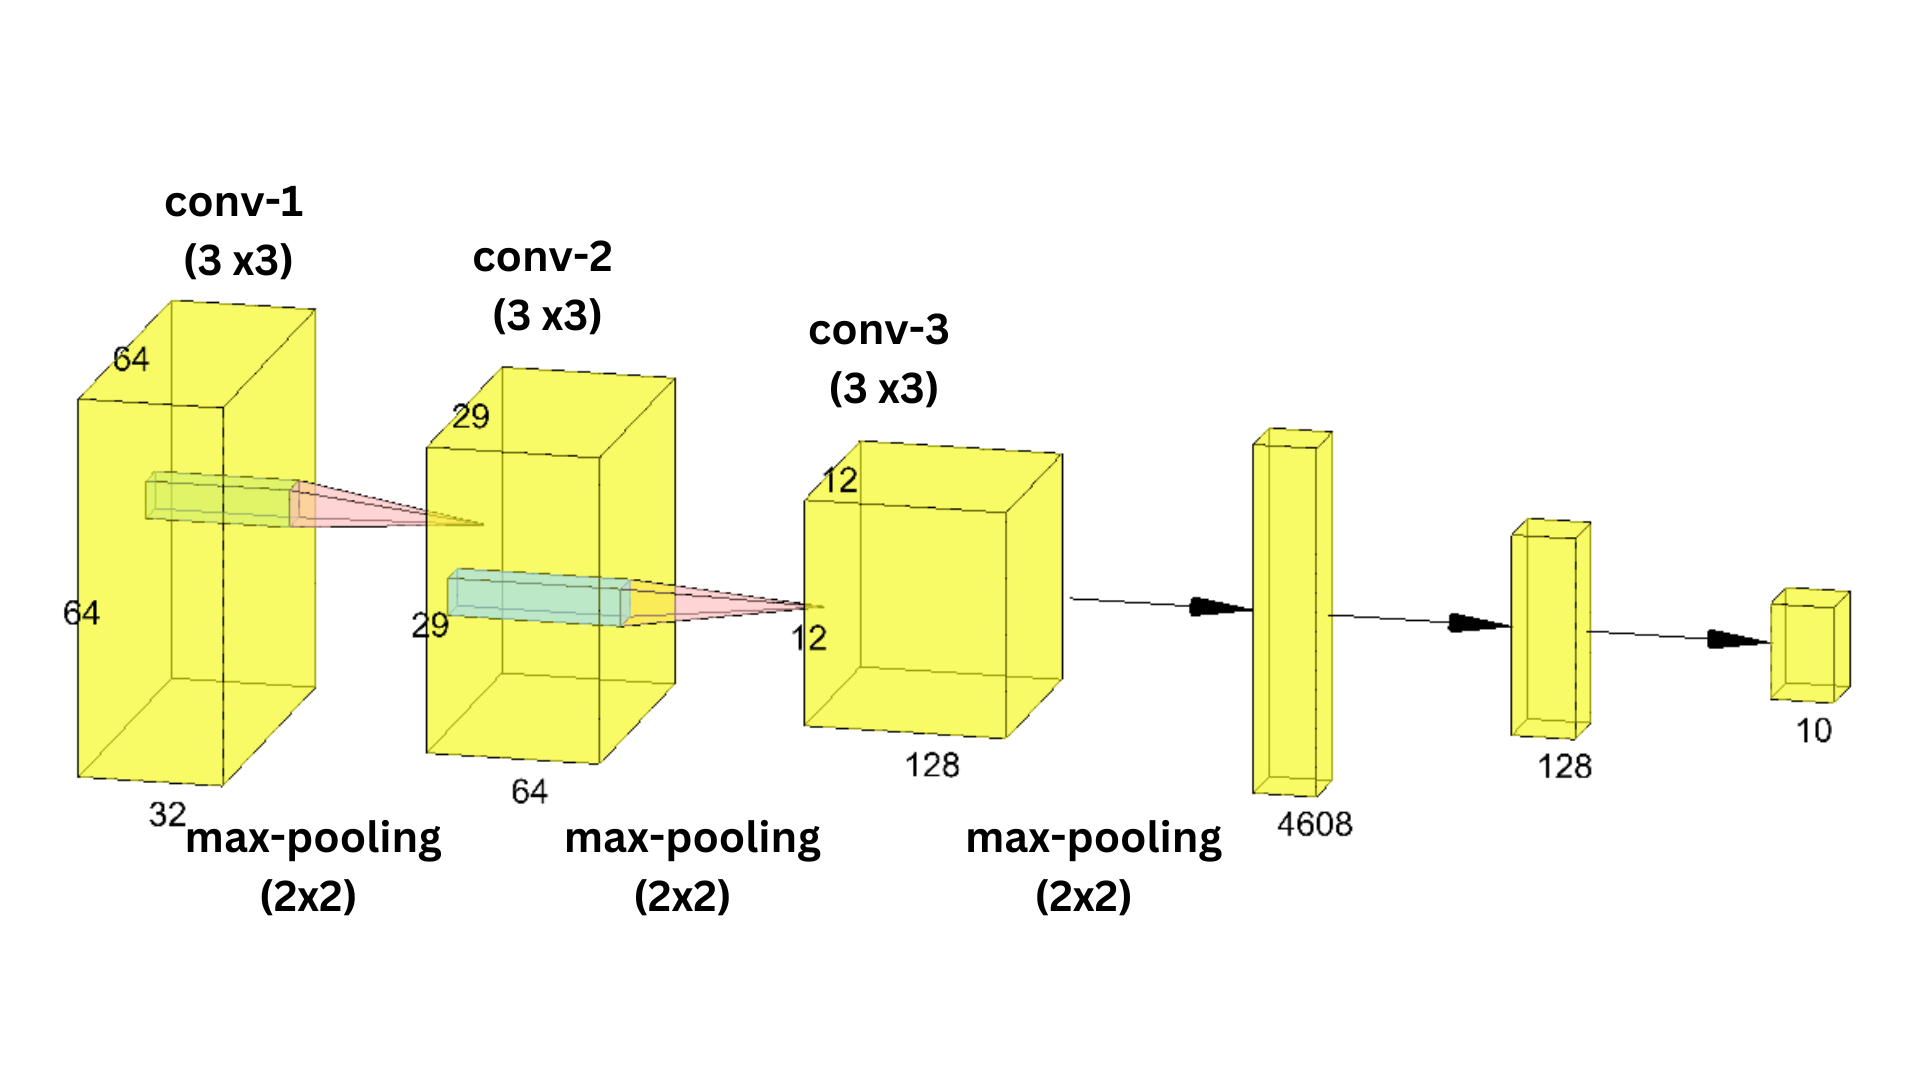
\includegraphics[width=0.75\textwidth]{imgs/p2ThidaNet.png}
\caption{Proposed Architecture for Myanmar handwritten digits Recognition.}\label{fig:p2Net}
\end{figure}

\begin{enumerate}
    \item \textbf{Input Layer}:
        \begin{itemize}
            \item The input layer is defined with the shape of $(64, 64, 1)$, accepts grayscale images of size $64 \times 64$ pixels.
        \end{itemize}
    
    \item \textbf{Convolutional Layers}:
        \begin{itemize}
            \item Three convolutional layers are added successively.
            \item The first layer has $32$ filters with a kernel size of $(3, 3)$ and ReLU activation function.
            \item The second layer has $64$ filters with the same kernel size and activation function.
            \item The third layer has $128$ filters with the same kernel size and activation function.
            \item After each convolutional layer, a max-pooling layer is applied with a pool size of $(2, 2)$, which helps in downsampling and extracting important features.
        \end{itemize}
    
    \item \textbf{Flatten Layer}:
        \begin{itemize}
            \item The output from the convolutional layers is flattened into a $1$D tensor, which will be fed into the fully connected layers.
        \end{itemize}
    
    \item \textbf{Fully Connected Layers}:
        \begin{itemize}
            \item There is a single fully connected hidden layer with $128$ neurons and ReLU activation function.
        \end{itemize}
    
    \item \textbf{Output Layer}:
        \begin{itemize}
            \item The output layer consists of $10$ neurons, representing the 10 classes of digits, with a softmax activation function. Softmax ensures that the output values are probabilities, summing up to $1$, which makes it suitable for multi-class classification tasks.
        \end{itemize}
    
    \item \textbf{Model Compilation}:
        \begin{itemize}
            \item The model is compiled using the Adam optimizer, categorical cross-entropy loss function (suitable for multi-class classification), and accuracy as the metric to monitor during training.
        \end{itemize}
\end{enumerate}

The proposed architecture has trainable parameters of 683,914 (2.61 MB) and the details breakdowns of the parameters for each layer is given below. 

Proposed လုပ်ထားသည့် Architecture တွင် feature များ ရယူရန်အတွက် convolutional နှင့် max-pooling layer များကို အသုံးပြုထားသည်။ convolutional layer သုံးခုတွင် 3x3 filter နှင့်  ReLU activation function ကို သုံးထားပြီး max-pooling layer တွင် 2x2 filter ကို အသုံးပြုသည်။ ထို့နောက် convolutional layer များမှ ရရှိလာသည့် output ကို flattened ပြုလုပ်ပြီး classification လုပ်ရန်အတွက် fully connected layer နှစ်ခုကို အသုံးပြုထားသည်။ နောက်ဆုံး output layer တွင် neuron (unit) ဆယ်ခုပါ၀င်ပြီး softmax activation function ကို အသုံးပြုထားသည်။ အဆိုပါ softmax function မှ  output ဆယ်ခု သည် မြန်မာ နံပါတ်တစ်ခုချင်းစီ၏ ဖြစ်နိုင်ချေ ရာခိုင်နှုန်းကို ညွှန်းဆိုသည်။ model ကို Compilation ပြုလုပ်ရန် Adam optimizer ကို အသုံးပြုထားပြီး accuracy တန်ဖိုးကို maximize လုပ်နိုင်သည့် parameter များကို ရှာဖွေစေခြင်းဖြစ်သည်။ 

ယခု model တွင် training ပြုလုပ်စဥ် ရှာဖွေရည့် parameter စုစုပေါင်း ခြောက်သိန်း ရှစ်သောင်း သုံးထောင် ကိုးရာ တစ်ဆယ့်လေးခု ရှိပြီး layer တစ်ခုချင်းစီတွက် လိုအပ်သည့် parameter အရေအတွက်ကို အောက်ပါဇယားတွင် ကြည့်ရှု့နိုင်သည်။ 

\vspace{0.5em}
\begin{figure}[h]%
\centering 
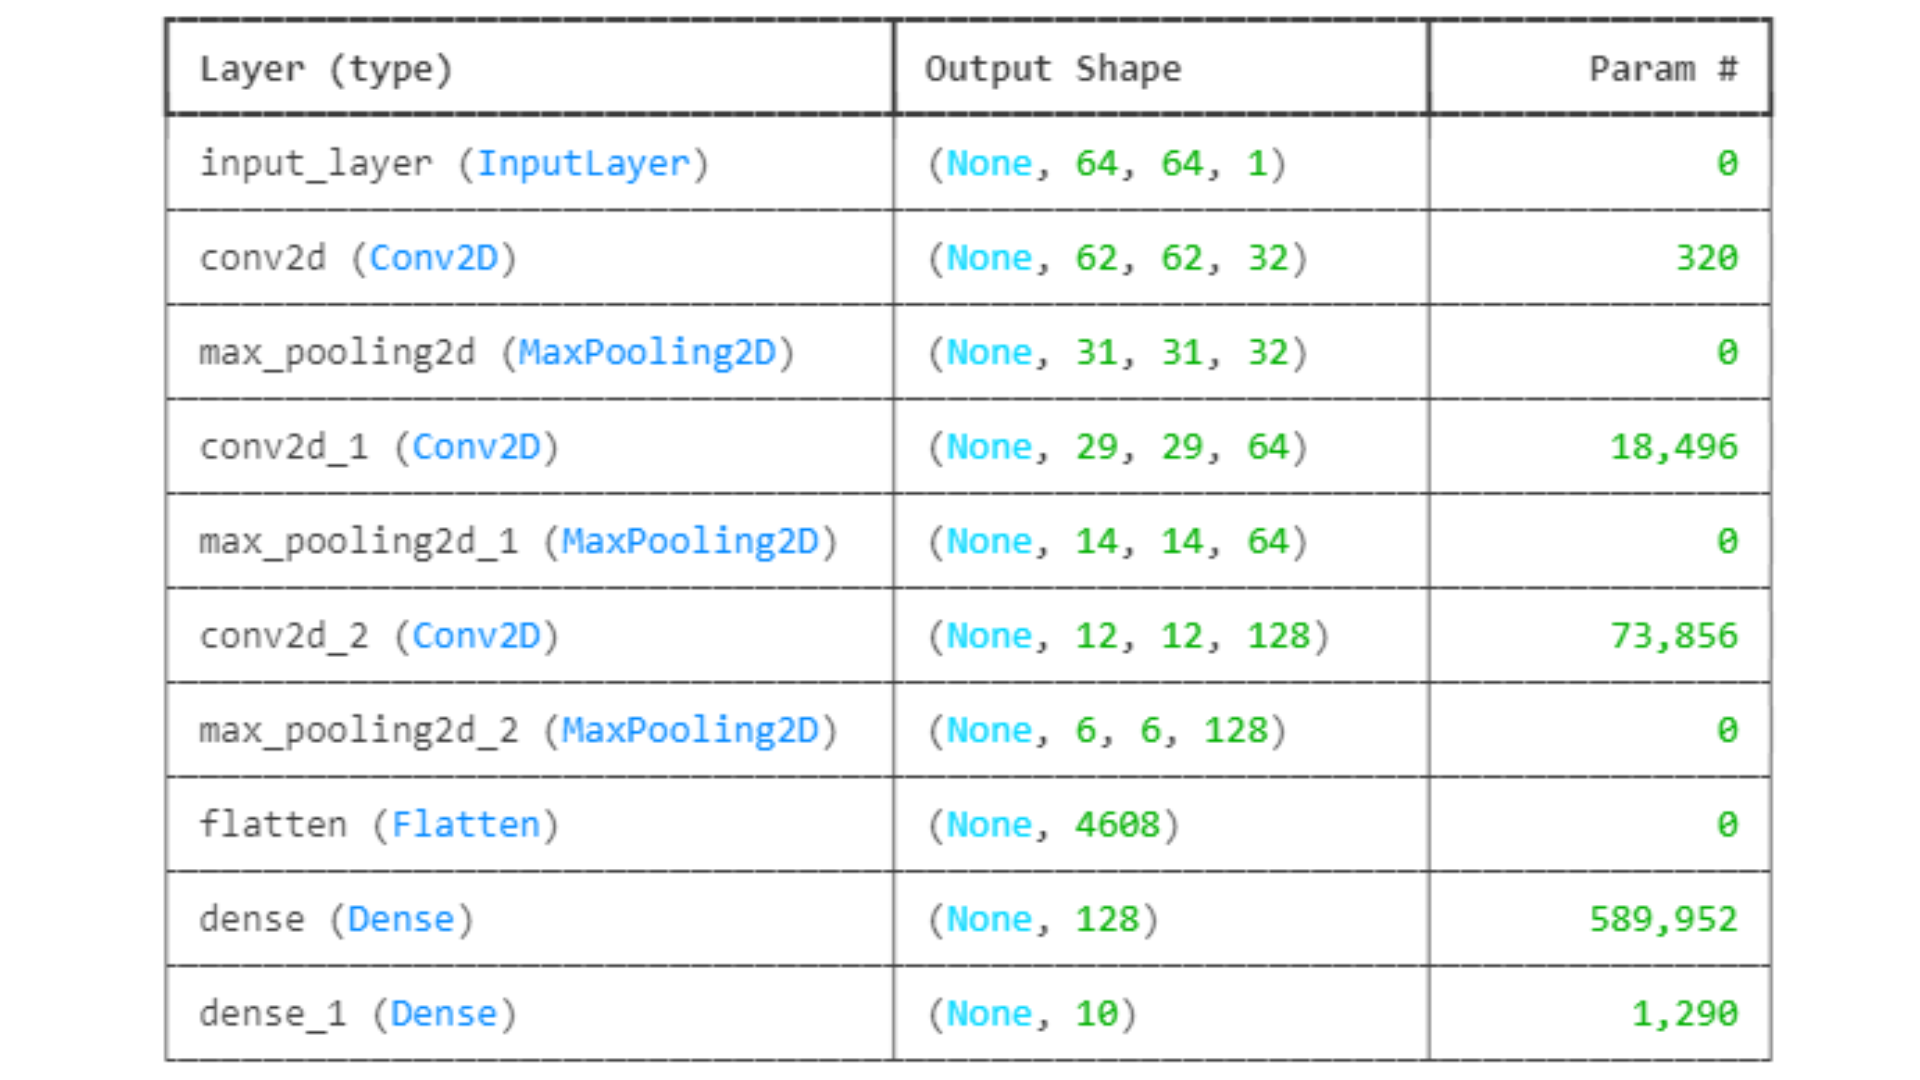
\includegraphics[width=0.75\textwidth]{imgs/p2_parameters.png}
\caption{Required Parameters for the Proposed Architecture.}\label{fig:p2Para}
\end{figure}
\subsubsection{Model Development}
This project comprises two Python scripts. The first script,\texttt{ `mmdigits.py'}, is responsible for extracting images from the specified data path and generating a substantial dataset along with a corresponding label vector, denoted as $X$ and $y$, respectively. The matrix X is formed as a large array of size $N x (64 x 64 x 1)$, where each row represents an individual image. Concurrently, the label vector $y$, with dimensions $Nx1$, contains the label for each corresponding row (or image) in $X$.

ဤ project တွင် ပါ၀င်သည့် code များကို Python file နှစ်ခုဖြင့် ပေးထားသည်။ ပထမ script \texttt{ `mmdigits.py'} တွင်  image များကို matrix အဖြစ် ဖန်တီခြင်းနှင့်၊  label များကို vector $y$ အဖြစ် တည်ဆောက်ခြင်း တို့ ပါ၀င်သည်။ ဒုတိယ script \texttt{HandDigit.ipynb} သည် အဓိက script ဖြစ်ပြီး deep learning model တည်ဆောက်ခြင်း၊ model ကို train ခြင်း နှင့် testing ပြုလုပ်ခြင်းတို့အပြင် ရလဒ်များကို သိမ်းဆည်းသည့် အပိုင်းတို့ ပါ၀င်သည်။ Python code များဖြစ်သည့်အတွက် မြန်မာ ဘာသာပြန်ဆိုခြင်း မပြုထားပါ။ 

\begin{solution}
\begin{lstlisting}
import os
import cv2
import numpy as np
def load_dataset(dataset_dir):
    images = []
    labels = []
    desired_width = 64
    desired_height = 64
    top_crop = 20
    bottom_crop = 20
    left_crop = 50
    right_crop = 50    
    # Loop through each subfolder in the dataset directory
    for class_label in os.listdir(dataset_dir):
        class_dir = os.path.join(dataset_dir, class_label)          
        # Check if it's a directory
        if os.path.isdir(class_dir):
            # Get the class label from the subfolder name
            label = int(class_label)
            # Loop through each image file in the subfolder
            for filename in os.listdir(class_dir):
                image_path = os.path.join(class_dir, filename)     
                # Read the image and convert it to grayscale
                image = cv2.imread(image_path, cv2.IMREAD_GRAYSCALE)
                # Crop and Resize image to a fixed size 
                image = image[top_crop:image.shape[0]-bottom_crop, 
                                    left_crop:image.shape[1]-right_crop]
                image = cv2.resize(image, (desired_width, desired_height))                
                # Add the image and label to the lists
                images.append(image)
                labels.append(label)

    # Convert lists to NumPy arrays
    images = np.array(images)
    labels = np.array(labels)    
    return images, labels
\end{lstlisting}  
\end{solution}

The second script, \texttt{HandDigit.ipynb}, is responsible for developing, training, and testing the deep learning model, as well as saving the results. 
In this script, two customized functions are first defined. The first function, \texttt{create\_cnn\_model(input\_shape)}, constructs the proposed architecture. The second function,\texttt{ save\_results} is responsible for saving the resulted confusion matrix and images. 

\begin{solution}
\begin{lstlisting}
def create_cnn_model(input_shape):    
    # Create an Input layer
    inputs = Input(shape=input_shape)    
    
    # Add convolutional layers
    x = Conv2D(32, kernel_size=(3, 3), activation='relu')(inputs)
    x = MaxPooling2D(pool_size=(2, 2))(x)
    x = Conv2D(64, kernel_size=(3, 3), activation='relu')(x)
    x = MaxPooling2D(pool_size=(2, 2))(x)
    x = Conv2D(128, kernel_size=(3, 3), activation='relu')(x)
    x = MaxPooling2D(pool_size=(2, 2))(x)    
    # Flatten the output from the convolutional layers
    x = Flatten()(x)    
    # Add fully connected layers
    x = Dense(128, activation='relu')(x)
    outputs = Dense(10, activation='softmax')(x)
    
    # Create the model
    model = Model(inputs=inputs, outputs=outputs)
    # Compile the model
    model.compile(optimizer='adam', loss='categorical_crossentropy', 
                        metrics=['accuracy'])   
    return model
\end{lstlisting}  
\end{solution}

\begin{solution}
\begin{lstlisting}
def save_results(y_test, y_pred, X_test, file_path):    

    result_conf  = confusion_matrix(y_test.argmax(axis=1), y_pred.argmax(axis=1))
    result_conf = pd.DataFrame(result_conf)
    result_conf.to_csv(file_path + 'cm.csv', index=False)    
    result_df = pd.DataFrame({'Test': y_test.argmax(axis=1), 
                                                'Pred': y_pred.argmax(axis=1)})
    result_df.to_csv(file_path + 'result.csv', index=False)  
    
    # Display the first image in the testing set
    idx = np.random.randint(0, X_test.shape[0])
    plt.imshow(X_test[idx], cmap='gray')
    plt.axis('off')
    plt.title(f"Predicted as: {y_pred[idx].argmax()} 
                            with percentage of {y_pred[idx].max()*100:.0f}%")
    num = y_test[idx].argmax()
    plt.savefig(file_path + str(num) + '.png', dpi = 100, bbox_inches = 'tight')
    plt.show()
\end{lstlisting}  
\end{solution}

Next, we explain the steps for developing and deploying the proposed deep learning model to classify the images into 10 different digits.
\setcounter{stepcounter}{0}
\begin{step}
The first step imports the required libraries, including the module customized module \texttt{`mmdigits'}. 
\begin{lstlisting}
from tensorflow import keras
from keras.datasets import mnist
from keras.models import Sequential, Model
from keras.utils import to_categorical, plot_model
from keras.layers import Input, Conv2D, MaxPooling2D, Flatten, Dense
from sklearn.metrics import confusion_matrix

import pydot, os
import pandas as pd
import numpy as np
import matplotlib.pyplot as plt
import mmdigits
from sklearn.model_selection import train_test_split
\end{lstlisting}  
\end{step}

\begin{step}
The second step creates a dataset for the images in the given directory using a function from the customized module \texttt{mmdigits}. This step generates a matrix, \texttt{images}, with a size of $N \times (64 \times 64)$, and a label vector, \texttt{labels}, with dimensions $N \times 1$, where each element corresponds to the label for each row (or image) in the \texttt{images} matrix. For the \texttt{Myanmar digits dataset}, $N$ is 2,200. The variable \texttt{`width'} and '\texttt{height}' decides the required image size for the proposed model. 

\begin{lstlisting}
dataset_dir = "./dataset/MM_digits/"
width = 64
height = 64
# Load the dataset
images, labels = mmdigits.load_dataset(dataset_dir)
\end{lstlisting}  
\end{step}

\begin{step}
Step 3 preprocesses the dataset. This step involves three key actions:
\begin{itemize}[b]
    \item The \texttt{images} matrix is reshaped to have dimensions $N \times (64 \times 64 \times 1)$, where each image is scaled to have pixel values between 0 and 1 by dividing by 255.0.
    \item The \texttt{labels} vector is converted to a one-hot encoded format using \texttt{keras.utils.to\_categorical}, which is essential for the classification task where the output layer has 10 neurons, one for each digit class.
    \item The dataset is then split into training and testing sets using \texttt{train\_test\_split}, with 30\% of the data allocated for testing and a random seed set for reproducibility.
\end{itemize}

\begin{lstlisting}
images = images.reshape(-1, width, height, 1).astype("float32") / 255.0
labels = keras.utils.to_categorical(labels, num_classes=10)
X_train, X_test, y_train, y_test = train_test_split(images, labels, 
                                                test_size=0.3, random_state=42)
\end{lstlisting}  
\end{step}

\begin{step}
Step 4 involves the training of the deep learning model.
\begin{lstlisting}
input_shape = (width,height,1)
model = create_cnn_model(input_shape)
model.fit(X_train, y_train, batch_size=128, epochs=10, validation_split=0.1, verbose=0)
y_pred = model.predict(X_test)
test_loss, test_accuracy = model.evaluate(X_test, y_test)
\end{lstlisting}  

\begin{itemize}[b]
    \item \texttt{input\_shape = (width,height,1)}: This line defines the input shape of the images for the model, which is required when constructing the convolutional neural network (CNN).
    \item \texttt{model = create\_cnn\_model(input\_shape)}: This line creates the CNN model using the previously defined function \texttt{create\_cnn\_model}, with the specified input shape.
    \item \texttt{model.fit(X\_train, y\_train, batch\_size=128, epochs=10, validation\_split=0.1, verbose=0)}: This line trains the model using the training data \texttt{X\_train} and labels \texttt{y\_train}. It specifies parameters such as batch size (128), number of epochs (10), validation split (10\% of training data), and verbosity level (0 for silent mode).
    \item \texttt{y\_pred = model.predict(X\_test)}: This line predicts the labels for the test data \texttt{X\_test} using the trained model.
    \item \texttt{test\_loss, test\_accuracy = model.evaluate(X\_test, y\_test)}: This line evaluates the performance of the model on the test data \texttt{X\_test} and corresponding labels \texttt{y\_test}. It returns the test loss and accuracy.
\end{itemize}
\end{step}

\begin{step}
Step 5 involves saving the results of the model evaluation. The first line specifies the directory path where the results will be saved. If the directory doesn't exist, it will be created by the second and third line by calling the \texttt{os.makedirs()} function under the \texttt{\textbf{os }}module. The last line saves the results of the model evaluation using the previously defined function \texttt{save\_results()}.  
\begin{lstlisting}
file_path = './results/mmdigit/'
if not os.path.exists(file_path):
    os.makedirs(file_path)
save_results(y_test, y_pred, X_test, file_path)
\end{lstlisting}  
\end{step}

\newpage
\subsubsection{Results and Discussion}

Figure \ref{fig:p2resutls} displays sample results of the model's predictions. The top row showcases correct predictions, accompanied by their corresponding confidence scores (probabilities). Conversely, the bottom row demonstrates instances where the model commonly misclassifies certain digits, such as 1 as 0, 0 as 8, 9 as 6, and 7 as 2.

အောက်ပါ ပုံတွင် proposed method ကို အသုံးပြု၍ ရရှိသည့် ရလဒ်များကို တင်ပြထားပါသည်။ ပထမ row တွင် အဖြေမှန်သည့် ရလဒ်များကို တင်ပြ၍ ဒုတိယ row မှားယွင်းသည့် ရလဒ်များကို ပြသထားသည်။ ဒုတိယ row၏ ပထမ ဆုံး နံပါတ်တွင် နံပါတ် \texttt{၁} ကို \texttt{၀} အဖြစ် လည်းကောင်း၊ ဒုတိယ ပုံတွင် \texttt{၀} ကို \texttt{၈} အဖြစ် လည်းကောင်း ၊ တတိယပုံတွင် \texttt{၉} ကို \texttt{၆} အဖြစ် လည်းကောင်း၊ နောက်ဆုံး ပုံတွင် \texttt{၇} ကို \texttt{၂ } အဖြစ် လည်းကောင်း မှားယွင်း ခန့်မှန်းထားသည်ကို တွေ့နိုင်သည်။ 

\vspace{0.5em}
\begin{figure}[h]%
\centering 
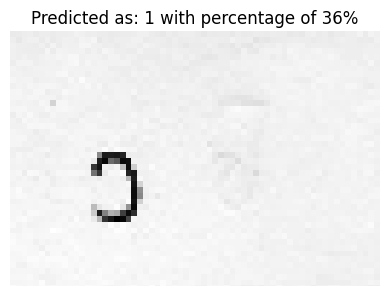
\includegraphics[width=0.225\textwidth]{imgs/1.png}
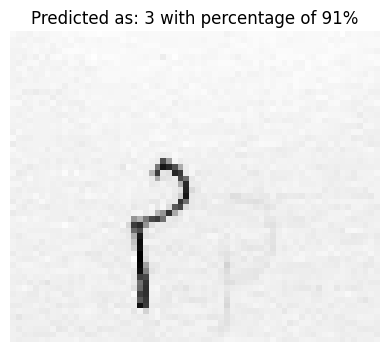
\includegraphics[width=0.22\textwidth]{imgs/3.png}
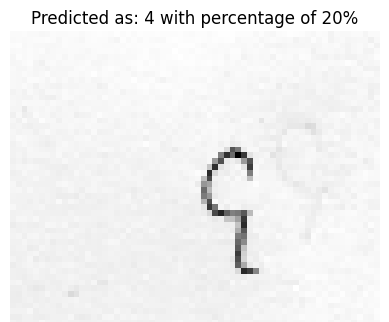
\includegraphics[width=0.225\textwidth]{imgs/4.png}
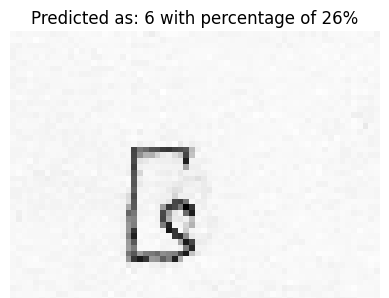
\includegraphics[width=0.225\textwidth]{imgs/6.png}
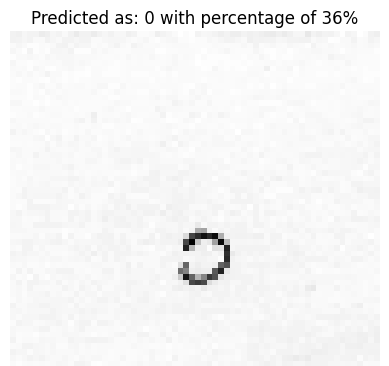
\includegraphics[width=0.225\textwidth]{imgs/1_0.png}
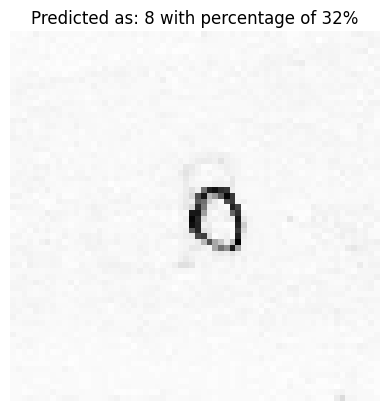
\includegraphics[width=0.22\textwidth]{imgs/0_8.png}
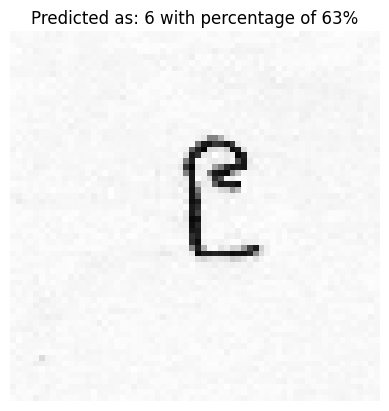
\includegraphics[width=0.22\textwidth]{imgs/9_6.png}
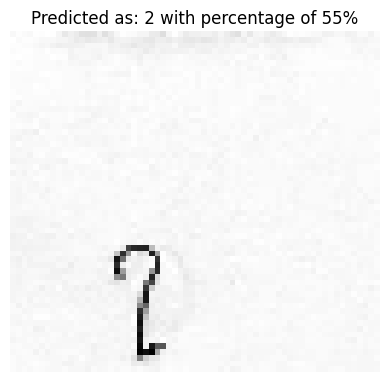
\includegraphics[width=0.225\textwidth]{imgs/7_2.png}
\caption{Sample Results of Myanmar Digits Recognition: Correct predictions (top) and incorrect predictions (bottom).}
\label{fig:p2resutls}
\end{figure}

\begin{figure}[h]
    \centering    
    \includegraphics[width=0.45\textwidth]{imgs/0and1.png}
    \includegraphics[width=0.5\textwidth]{imgs/2and7.png}
    \includegraphics[width=0.45\textwidth]{imgs/5and9.png}
    \caption{Similarity between Myanmar digits `0' \& `1',  `2' \& '7', and '5' \& `9'.}
    \label{fig:mm_digits_similarity}
\end{figure}

ဤသို့ မှားယွင်း ခန့်မှန်းရသည့် အကြောင်းရင်းမှာ မြန်မာ နံပါတ်များ၏ ဆင်တူမှု ကြောင့်ဖြစ်သည်။ မြန်မာ နံပါတ်များတွင် သုည နှင့် တစ်သည် လက်ရေးသော့သူ ဖြစ်ပါက ခွဲခြားရန် ခက်ခဲသည်ကို အထက်ပါပုံတွင် တွေ့နိုင်ပါသည်။ ထို့အပြင် \texttt{၉} ၊  \texttt{၆} နှင့် \texttt{၅} တို့သည်လည် ပြောင်းပြန် လှည့်လိုက်ပါက လက်ရေးမူတွင် ထပ်တူ နီးပါး ကျနေသည်ကို တွေ့နိုင်သည်။ အောက်ပါ ဇယားတွင် testing result အတွက် ရရှိသည့် confusion matrix ကို ပြသထားပါသည်။ ပထမ row ကို ကြည့်မည်ဆိုပါက သုညကို ရှစ် အဖြစ် မှားယွင်းခန့်မှန်းထားသည့် အကြိမ်ပေါင်း နှစ်ဆယ့်ကိုး ကြိမ် ရှိသည်ကို တွေ့နိုင်ပါသည်။ သုညကို တစ်အဖြစ် မှားယွင်းမှုသည် လေး ကြိမ်သာ ဖြစ်ခဲ့သော်လည်း တစ်ကို သုည အဖြစ် မှားယွင်းမှုသည် အကြိမ် နှစ်ဆယ် ခန့် ရှိသည်ကို တွေ့ နိုင်သည်။ accuracy score မှာ ၆၀ ရာခိုင်နှုန်း ရရှိရာ ယေဘူယျ အားဖြင့် ရလဒ်သည် မဆိုးဟု ဆိုနိုင်သော်လည်း ပိုမို ကောင်းမွန်သည့် ရလဒ်များကို ရရှိနိုင်ရန် လိုအပ်နေသေးသည်။ 

Table \ref{tab:p2cm} presents the confusion matrix for the MM digits dataset. Each row represents the true label of the samples, while each column represents the predicted label by the proposed model. Notably, certain digits such as '0' and '1', as well as '6' and '9', are frequently misclassified, leading to overall accuracy score of 60\%. This is likely due to the similarities between these digits in handwritten Myanmar script, as illustrated in Figure \ref{fig:mm_digits_similarity}. 

\vspace{0.5em}
\begin{table}[h]
    \centering
    \begin{tabular}{|*{11}{c|}}
        \hline 
        & 0 & 1 & 2 & 3 & 4 & 5 & 6 & 7 & 8 & 9 \\
        \hline
        0 & \colorbox{yellow}{25} & 4 & 1 & 1 & 1 & 0 & 0 & 2 & 29 & 2 \\\hline
        1 & 20 & \colorbox{yellow}{35} & 3 & 5 & 0 & 0 & 0 & 2 & 10 & 2 \\\hline
        2 & 1 & 4 & \colorbox{yellow}{59} & 6 & 1 & 0 & 0 & 0 & 1 & 0 \\\hline
        3 & 0 & 4 & 1 & \colorbox{yellow}{45} & 9 & 0 & 1 & 1 & 0 & 1 \\\hline
        4 & 0 & 1 & 1 & 12 & \colorbox{yellow}{37} & 0 & 3 & 5 & 0 & 1 \\\hline
        5 & 0 & 0 & 1 & 2 & 12 & \colorbox{yellow}{18} & 4 & 9 & 3 & 13 \\\hline
        6 & 2 & 1 & 0 & 1 & 1 & 0 & \colorbox{yellow}{40} & 2 & 4 & 4 \\\hline
        7 & 0 & 2 & 0 & 2 & 10 & 0 & 2 & \colorbox{yellow}{50} & 1 & 2 \\\hline
        8 & 17 & 1 & 0 & 1 & 0 & 0 & 3 & 1 & \colorbox{yellow}{45} & 5 \\\hline
        9 & 1 & 3 & 1 & 9 & 1 & 0 & 8 & 4 & 1 & \colorbox{yellow}{43} \\
        \hline
    \end{tabular}
    \caption{Confusion matrix for Myanmar Handwritten digits recognition}
    \label{tab:p2cm}
\end{table}


In future work, efforts could focus on enhancing the model's performance by addressing the challenges observed in the confusion matrix presented in Table 
\ref{tab:p2cm}. Specifically, attention could be given to addressing the challenges posed by the similarities between certain digits in the handwritten Myanmar script, as illustrated in Figure \ref{fig:mm_digits_similarity}. One possible avenue for future work is collecting additional training data for these digits and augmenting the dataset with variations in handwriting styles. Additionally, fine-tuning hyperparameters and exploring alternative neural network architectures tailored to capture the intricacies of handwritten Myanmar script could be beneficial.

လက်ရေးဖြင့် ရေးထားသည့် မြန်မာ နံပါတ်များကို recognize ပြုလုပ်ခြင်းသည် မြန်မာ နည်းပညာလောက ပိုမို တိုးတက်စေရန် အရေးကြီးသည့် Project တစ်ခု ဖြစ်ပါသည်။ ယခု သင်ခန်းစာတွင် စာဖတ်သူများ အတွက် လွယ်ကူစေရန် ရိုးရှင်းသည့် deep learning model တစ်ခုကို အသုံးပြု၍ ရလဒ်များကို တင်ပြထားသော်လည်း ပိုမို ကောင်းမွန်သည့် model များကို တီထွင်သင့်ပါသည်။ ရလဒ်ကောင်းများ ရရှိနိုင်စေရန် လက်ရေး အမျိုးမျိုး ဖြင့် ရေးသားထားသည့် ဒေတာများကို ထပ်မံ စုဆောင်းခြင်း၊ model ၏ architecture ကို ပိုမိုကောင်းမွန်အောင် ပြုလုပ်ခြင်းများ ပြုလုပ်ရန် တိုက်တွန်းအပ်ပါသည်။ 

\newpage
\section{Chapter-End Exercises}\label{sec:exercises}
\begin{question}
What is one of the primary benefits of using deep learning networks over traditional (shallow) neural networks?
\begin{enumerate}[a] % Alphabetical enumeration
    \item Reduced computational resources needed for training
    \item Ability to learn hierarchical representations of data
    \item Easier to interpret and understand    
\end{enumerate}
\end{question} 

\begin{answer}
The correct answer is \texttt{Ability to learn hierarchical representations of data}. Deep learning networks excel at learning hierarchical representations of data, allowing them to capture complex patterns and features that may not be easily discernible with traditional neural networks.
\end{answer}

\begin{question}
What is the primary function of the pooling layer in a Convolutional Neural Network (CNN)?
\begin{enumerate}[a]
\item To increase the spatial dimensions of the feature maps
\item To reduce the spatial dimensions of the feature maps
\item To adjust the weights connecting the hidden layer to the output layer
\end{enumerate}
\end{question} 

\begin{question}
Which layer in a CNN connects every neuron in one layer to every neuron in the next layer, similar to traditional artificial neural networks?
\begin{enumerate}[a]
\item Input Layer
\item Convolutional Layer
\item Fully Connected Layer
\end{enumerate}
\end{question}

\begin{question}
What is the role of the output layer in a CNN for a classification task?
\begin{enumerate}[a]
\item To produce a continuous output value
\item To learn hierarchical representations of data
\item To represent the probability of the input belonging to each class
\end{enumerate}
\end{question} 
\chapter{Recurrent Neural Networks (RNNs)}\label{sec:RNN}
This section introduces RNNs, a class of neural networks capable of modeling sequential data. It discusses the architecture of RNNs, including recurrent layers and different variants such as Long Short-Term Memory (LSTM) and Gated Recurrent Unit (GRU). Practical examples illustrate how RNNs can be used for tasks such as natural language processing, time-series forecasting, and sentiment analysis. 

\section{Long Short-Term Memory (LSTM) Networks}

\subsection{Case Study 1: Time Series Prediction}

\subsection{Case Study 2: Feedback sentiment analysis}

Feedback sentiment analysis is the process of using natural language processing (NLP) and machine learning techniques to determine the sentiment expressed in user feedback. The goal is to classify the feedback into categories such as positive, negative, or neutral, allowing businesses to gain insights into customer satisfaction and areas for improvement.

\begin{remark}
This work is inspired by a project assignment given to my Master students. In this course, students were tasked with developing a classification model to identify. While the codes and explanations are my original work, the project context was developed as part of the coursework to provide practical learning experiences.
\end{remark}

\section{Autoencoders}\label{sec:autoencoder}
Autoencoders are neural networks trained to reproduce their input data at the output layer. They consist of an encoder network that compresses the input data into a lower-dimensional representation (encoding) and a decoder network that reconstructs the original input from the encoding. Autoencoders are used for tasks such as dimensionality reduction, data denoising, and anomaly detection.

\section{Transformers}\label{sec:transformers}

Transformers are a type of deep learning architecture that has gained significant popularity in natural language processing (NLP) tasks. Introduced by Vaswani et al. in the paper "Attention is All You Need," transformers have revolutionized NLP by achieving state-of-the-art performance on a wide range of tasks.

The key innovation of transformers lies in their self-attention mechanism, which allows them to capture long-range dependencies in sequential data more effectively than traditional recurrent neural networks (RNNs) and convolutional neural networks (CNNs). Unlike RNNs, transformers process input data in parallel, making them highly efficient for training on large datasets.

\section{Generative Adversarial Networks (GANs)}\label{sec:GAN} 
\subsection{Generative Adversarial Networks (GANs)}

\subsection{Reinforcement Learning (RL)}

\subsection{Integration of GANs and RL} 

\newpage



\section{Further Reading}

\subsection{Courses and Lecture Notes}
\begin{enumerate}[1] 
    \item Prof. Philippe Rigollet, Mathematics Of Machine Learning, MIT OpenCourse \url{https://ocw.mit.edu/courses/18-657-mathematics-of-machine-learning-fall-2015/}
\end{enumerate}

\subsection{Books}
\begin{enumerate}[1] 
    \item Shalev-Shwartz, Shai, and Shai Ben-David. Understanding Machine Learning: From Theory to Algorithms. Cambridge University Press, 2014. ISBN: 9781107057135
\end{enumerate}

\subsection{Leading Journal and Conferences}

\begin{enumerate}[1] 
    \item The International Conference on Machine Learning (ICML)
    \item The Conference on Neural Information Processing Systems (NeurIPS)     
\end{enumerate}


\chapter{ Emerging Trends in Deep Learning}

\subsection{Transfer Learning and Fine-Tuning}\label{sec:transfer}

\subsection{Attention Mechanisms and Transformers}\label{sec:transfomers}

\subsection{AutoML and Neural Architecture Search (NAS)}\label{sec:NAS}

\subsection{Ethical Considerations and Bias in Deep Learning}\label{sec:ethic}

\bibliographystyle{unsrt} % We choose the "plain" reference style
\bibliography{refs_deep}
%\chapter{Title chapter 1}
%
%\section{section Title}
%
%\begin{definition}
%    Hello world
%\end{definition}
%
%\begin{remark}
%    This is remark
%\end{remark}
%
%\begin{example}
%    this is example
%\end{example}
%
%\chapter{Chapter Title Here}
%% Chapter content goes here.
%this is chapter
%\section{Section Title Here}
%% Section content goes here.
%this is section
%\subsection{Subsection Title Here}
%% Subsection content goes here.
%this is subsection
%\subsubsection{Subsubsection Title Here}
%% Subsubsection content goes here.
%this is subsection
%\begin{activity}
%Your activity content here.
%\end{activity}
%
%\begin{definition}
%Your definition content here.
%\end{definition}
%
%\begin{theorem}
%Your theorem content here.
%\end{theorem}
%
%\begin{example}
%Your example content here.
%\end{example}
%
%\begin{exercise}
%Your exercise content here.
%\end{exercise}
%
%\begin{generality}
%Your generality content here.
%\end{generality}
%
%\begin{property}
%Your property content here.
%\end{property}
%
%\begin{solution}
%Your solution content here.
%\end{solution}
%
%\begin{remark}
%Your remark content here.
%\end{remark}
%
%% Demonstration of customized lists
%\begin{enumerate}[1] % Default numeric enumeration
%    \item First item.
%    \item Second item.
%\end{enumerate}
%
%\begin{enumerate}[a] % Alphabetical enumeration
%    \item First item.
%    \item Second item.
%\end{enumerate}
%
%\begin{itemize}[f1] % Custom itemize with specific symbol
%    \item First item.
%    \item Second item.
%\end{itemize}
%
%\begin{itemize}[b] % Bullet points
%    \item First bullet point.
%    \item Second bullet point.
%\end{itemize}
%
%% Example of a multicolumn enumeration
%\begin{Enumerate}(2) % Two-column enumerate
%    \item First item in two-column list.
%    \item Second item in two-column list.
%\end{Enumerate}
%
%% Custom tasks (similar to itemize or enumerate)
%\begin{tasks}(2)
% Two-column tasks
%    \task First task.
%    \task Second task.
%\end{tasks}

\end{document}

\blinddocument
